\documentclass[twoside]{book}

% Packages required by doxygen
\usepackage{calc}
\usepackage{doxygen}
\usepackage{graphicx}
\usepackage[utf8]{inputenc}
\usepackage{makeidx}
\usepackage{multicol}
\usepackage{multirow}
\usepackage{textcomp}
\usepackage[table]{xcolor}

% Font selection
\usepackage[T1]{fontenc}
\usepackage{mathptmx}
\usepackage[scaled=.90]{helvet}
\usepackage{courier}
\usepackage{amssymb}
\usepackage{sectsty}
\renewcommand{\familydefault}{\sfdefault}
\allsectionsfont{%
  \fontseries{bc}\selectfont%
  \color{darkgray}%
}
\renewcommand{\DoxyLabelFont}{%
  \fontseries{bc}\selectfont%
  \color{darkgray}%
}

% Page & text layout
\usepackage{geometry}
\geometry{%
  a4paper,%
  top=2.5cm,%
  bottom=2.5cm,%
  left=2.5cm,%
  right=2.5cm%
}
\tolerance=750
\hfuzz=15pt
\hbadness=750
\setlength{\emergencystretch}{15pt}
\setlength{\parindent}{0cm}
\setlength{\parskip}{0.2cm}
\makeatletter
\renewcommand{\paragraph}{%
  \@startsection{paragraph}{4}{0ex}{-1.0ex}{1.0ex}{%
    \normalfont\normalsize\bfseries\SS@parafont%
  }%
}
\renewcommand{\subparagraph}{%
  \@startsection{subparagraph}{5}{0ex}{-1.0ex}{1.0ex}{%
    \normalfont\normalsize\bfseries\SS@subparafont%
  }%
}
\makeatother

% Headers & footers
\usepackage{fancyhdr}
\pagestyle{fancyplain}
\fancyhead[LE]{\fancyplain{}{\bfseries\thepage}}
\fancyhead[CE]{\fancyplain{}{}}
\fancyhead[RE]{\fancyplain{}{\bfseries\leftmark}}
\fancyhead[LO]{\fancyplain{}{\bfseries\rightmark}}
\fancyhead[CO]{\fancyplain{}{}}
\fancyhead[RO]{\fancyplain{}{\bfseries\thepage}}
\fancyfoot[LE]{\fancyplain{}{}}
\fancyfoot[CE]{\fancyplain{}{}}
\fancyfoot[RE]{\fancyplain{}{\bfseries\scriptsize Generated on Mon Mar 21 2016 07\-:50\-:31 for S\-V\-Prog by Doxygen }}
\fancyfoot[LO]{\fancyplain{}{\bfseries\scriptsize Generated on Mon Mar 21 2016 07\-:50\-:31 for S\-V\-Prog by Doxygen }}
\fancyfoot[CO]{\fancyplain{}{}}
\fancyfoot[RO]{\fancyplain{}{}}
\renewcommand{\footrulewidth}{0.4pt}
\renewcommand{\chaptermark}[1]{%
  \markboth{#1}{}%
}
\renewcommand{\sectionmark}[1]{%
  \markright{\thesection\ #1}%
}

% Indices & bibliography
\usepackage{natbib}
\usepackage[titles]{tocloft}
\setcounter{tocdepth}{3}
\setcounter{secnumdepth}{5}
\makeindex

% Hyperlinks (required, but should be loaded last)
\usepackage{ifpdf}
\ifpdf
  \usepackage[pdftex,pagebackref=true]{hyperref}
\else
  \usepackage[ps2pdf,pagebackref=true]{hyperref}
\fi
\hypersetup{%
  colorlinks=true,%
  linkcolor=blue,%
  citecolor=blue,%
  unicode%
}

% Custom commands
\newcommand{\clearemptydoublepage}{%
  \newpage{\pagestyle{empty}\cleardoublepage}%
}


%===== C O N T E N T S =====

\begin{document}

% Titlepage & ToC
\hypersetup{pageanchor=false}
\pagenumbering{roman}
\begin{titlepage}
\vspace*{7cm}
\begin{center}%
{\Large S\-V\-Prog }\\
\vspace*{1cm}
{\large Generated by Doxygen 1.8.6}\\
\vspace*{0.5cm}
{\small Mon Mar 21 2016 07:50:31}\\
\end{center}
\end{titlepage}
\clearemptydoublepage
\tableofcontents
\clearemptydoublepage
\pagenumbering{arabic}
\hypersetup{pageanchor=true}

%--- Begin generated contents ---
\chapter{Namespace Index}
\section{Namespace List}
Here is a list of all namespaces with brief descriptions\-:\begin{DoxyCompactList}
\item\contentsline{section}{\hyperlink{namespacej}{j} }{\pageref{namespacej}}{}
\item\contentsline{section}{\hyperlink{namespacej_1_1impl}{j\-::impl} }{\pageref{namespacej_1_1impl}}{}
\item\contentsline{section}{\hyperlink{namespaces}{s} }{\pageref{namespaces}}{}
\end{DoxyCompactList}

\chapter{Hierarchical Index}
\section{Class Hierarchy}
This inheritance list is sorted roughly, but not completely, alphabetically\-:\begin{DoxyCompactList}
\item \contentsline{section}{j\-:\-:impl\-:\-:Abstract\-Value}{\pageref{classj_1_1impl_1_1_abstract_value}}{}
\begin{DoxyCompactList}
\item \contentsline{section}{j\-:\-:impl\-:\-:Array}{\pageref{classj_1_1impl_1_1_array}}{}
\item \contentsline{section}{j\-:\-:impl\-:\-:Boolean}{\pageref{classj_1_1impl_1_1_boolean}}{}
\item \contentsline{section}{j\-:\-:impl\-:\-:Number}{\pageref{classj_1_1impl_1_1_number}}{}
\item \contentsline{section}{j\-:\-:impl\-:\-:Object}{\pageref{classj_1_1impl_1_1_object}}{}
\item \contentsline{section}{j\-:\-:impl\-:\-:String}{\pageref{classj_1_1impl_1_1_string}}{}
\end{DoxyCompactList}
\item \contentsline{section}{Application}{\pageref{class_application}}{}
\begin{DoxyCompactList}
\item \contentsline{section}{Final\-Application}{\pageref{class_final_application}}{}
\item \contentsline{section}{World\-Test}{\pageref{class_world_test}}{}
\end{DoxyCompactList}
\item \contentsline{section}{j\-:\-:Value\-:\-:Array\-Tag}{\pageref{structj_1_1_value_1_1_array_tag}}{}
\item \contentsline{section}{Collider}{\pageref{class_collider}}{}
\begin{DoxyCompactList}
\item \contentsline{section}{Body}{\pageref{class_body}}{}
\end{DoxyCompactList}
\item \contentsline{section}{Drawable}{\pageref{class_drawable}}{}
\item logic\-\_\-error\begin{DoxyCompactList}
\item \contentsline{section}{j\-:\-:Bad\-Conversion}{\pageref{classj_1_1_bad_conversion}}{}
\item \contentsline{section}{j\-:\-:No\-Such\-Element}{\pageref{classj_1_1_no_such_element}}{}
\end{DoxyCompactList}
\item \contentsline{section}{j\-:\-:Value\-:\-:Object\-Tag}{\pageref{structj_1_1_value_1_1_object_tag}}{}
\item runtime\-\_\-error\begin{DoxyCompactList}
\item \contentsline{section}{j\-:\-:Bad\-Payload}{\pageref{classj_1_1_bad_payload}}{}
\item \contentsline{section}{j\-:\-:No\-Such\-File}{\pageref{classj_1_1_no_such_file}}{}
\end{DoxyCompactList}
\item \contentsline{section}{Updatable}{\pageref{class_updatable}}{}
\item \contentsline{section}{j\-:\-:Value}{\pageref{classj_1_1_value}}{}
\item \contentsline{section}{Vec2d}{\pageref{class_vec2d}}{}
\item \contentsline{section}{World}{\pageref{class_world}}{}
\end{DoxyCompactList}

\chapter{Class Index}
\section{Class List}
Here are the classes, structs, unions and interfaces with brief descriptions\-:\begin{DoxyCompactList}
\item\contentsline{section}{\hyperlink{classj_1_1impl_1_1_abstract_value}{j\-::impl\-::\-Abstract\-Value} }{\pageref{classj_1_1impl_1_1_abstract_value}}{}
\item\contentsline{section}{\hyperlink{class_application}{Application} \\*Abstract class managing the core of the program }{\pageref{class_application}}{}
\item\contentsline{section}{\hyperlink{classj_1_1impl_1_1_array}{j\-::impl\-::\-Array} }{\pageref{classj_1_1impl_1_1_array}}{}
\item\contentsline{section}{\hyperlink{structj_1_1_value_1_1_array_tag}{j\-::\-Value\-::\-Array\-Tag} }{\pageref{structj_1_1_value_1_1_array_tag}}{}
\item\contentsline{section}{\hyperlink{classj_1_1_bad_conversion}{j\-::\-Bad\-Conversion} }{\pageref{classj_1_1_bad_conversion}}{}
\item\contentsline{section}{\hyperlink{classj_1_1_bad_payload}{j\-::\-Bad\-Payload} }{\pageref{classj_1_1_bad_payload}}{}
\item\contentsline{section}{\hyperlink{class_body}{Body} }{\pageref{class_body}}{}
\item\contentsline{section}{\hyperlink{classj_1_1impl_1_1_boolean}{j\-::impl\-::\-Boolean} }{\pageref{classj_1_1impl_1_1_boolean}}{}
\item\contentsline{section}{\hyperlink{class_collider}{Collider} }{\pageref{class_collider}}{}
\item\contentsline{section}{\hyperlink{class_drawable}{Drawable} \\*Represents an entity that can be represented graphically }{\pageref{class_drawable}}{}
\item\contentsline{section}{\hyperlink{class_final_application}{Final\-Application} }{\pageref{class_final_application}}{}
\item\contentsline{section}{\hyperlink{classj_1_1_no_such_element}{j\-::\-No\-Such\-Element} }{\pageref{classj_1_1_no_such_element}}{}
\item\contentsline{section}{\hyperlink{classj_1_1_no_such_file}{j\-::\-No\-Such\-File} }{\pageref{classj_1_1_no_such_file}}{}
\item\contentsline{section}{\hyperlink{classj_1_1impl_1_1_number}{j\-::impl\-::\-Number} }{\pageref{classj_1_1impl_1_1_number}}{}
\item\contentsline{section}{\hyperlink{classj_1_1impl_1_1_object}{j\-::impl\-::\-Object} }{\pageref{classj_1_1impl_1_1_object}}{}
\item\contentsline{section}{\hyperlink{structj_1_1_value_1_1_object_tag}{j\-::\-Value\-::\-Object\-Tag} }{\pageref{structj_1_1_value_1_1_object_tag}}{}
\item\contentsline{section}{\hyperlink{classj_1_1impl_1_1_string}{j\-::impl\-::\-String} }{\pageref{classj_1_1impl_1_1_string}}{}
\item\contentsline{section}{\hyperlink{class_updatable}{Updatable} \\*Represents an entity that evolves with time }{\pageref{class_updatable}}{}
\item\contentsline{section}{\hyperlink{classj_1_1_value}{j\-::\-Value} }{\pageref{classj_1_1_value}}{}
\item\contentsline{section}{\hyperlink{class_vec2d}{Vec2d} \\*Bridge vector class to sf\-::\-Vector2i/f that provides some common math methods }{\pageref{class_vec2d}}{}
\item\contentsline{section}{\hyperlink{class_world}{World} }{\pageref{class_world}}{}
\item\contentsline{section}{\hyperlink{class_world_test}{World\-Test} }{\pageref{class_world_test}}{}
\end{DoxyCompactList}

\chapter{File Index}
\section{File List}
Here is a list of all files with brief descriptions\-:\begin{DoxyCompactList}
\item\contentsline{section}{/home/jbesson/myfiles/cpp/svprog/partie1/src/\hyperlink{_application_8cpp}{Application.\-cpp} }{\pageref{_application_8cpp}}{}
\item\contentsline{section}{/home/jbesson/myfiles/cpp/svprog/partie1/src/\hyperlink{_application_8hpp}{Application.\-hpp} }{\pageref{_application_8hpp}}{}
\item\contentsline{section}{/home/jbesson/myfiles/cpp/svprog/partie1/src/\hyperlink{_config_8hpp}{Config.\-hpp} }{\pageref{_config_8hpp}}{}
\item\contentsline{section}{/home/jbesson/myfiles/cpp/svprog/partie1/src/\hyperlink{_final_application_8cpp}{Final\-Application.\-cpp} }{\pageref{_final_application_8cpp}}{}
\item\contentsline{section}{/home/jbesson/myfiles/cpp/svprog/partie1/src/\hyperlink{_final_application_8hpp}{Final\-Application.\-hpp} }{\pageref{_final_application_8hpp}}{}
\item\contentsline{section}{/home/jbesson/myfiles/cpp/svprog/partie1/src/\-Env/\hyperlink{_collider_8cpp}{Collider.\-cpp} }{\pageref{_collider_8cpp}}{}
\item\contentsline{section}{/home/jbesson/myfiles/cpp/svprog/partie1/src/\-Env/\hyperlink{_collider_8hpp}{Collider.\-hpp} }{\pageref{_collider_8hpp}}{}
\item\contentsline{section}{/home/jbesson/myfiles/cpp/svprog/partie1/src/\-Env/\hyperlink{_world_8hpp}{World.\-hpp} }{\pageref{_world_8hpp}}{}
\item\contentsline{section}{/home/jbesson/myfiles/cpp/svprog/partie1/src/\-Interface/\hyperlink{_drawable_8hpp}{Drawable.\-hpp} }{\pageref{_drawable_8hpp}}{}
\item\contentsline{section}{/home/jbesson/myfiles/cpp/svprog/partie1/src/\-Interface/\hyperlink{_updatable_8hpp}{Updatable.\-hpp} }{\pageref{_updatable_8hpp}}{}
\item\contentsline{section}{/home/jbesson/myfiles/cpp/svprog/partie1/src/\-J\-S\-O\-N/\hyperlink{_j_s_o_n_8cpp}{J\-S\-O\-N.\-cpp} }{\pageref{_j_s_o_n_8cpp}}{}
\item\contentsline{section}{/home/jbesson/myfiles/cpp/svprog/partie1/src/\-J\-S\-O\-N/\hyperlink{_j_s_o_n_8hpp}{J\-S\-O\-N.\-hpp} }{\pageref{_j_s_o_n_8hpp}}{}
\item\contentsline{section}{/home/jbesson/myfiles/cpp/svprog/partie1/src/\-J\-S\-O\-N/\hyperlink{_j_s_o_n_impl_8cpp}{J\-S\-O\-N\-Impl.\-cpp} }{\pageref{_j_s_o_n_impl_8cpp}}{}
\item\contentsline{section}{/home/jbesson/myfiles/cpp/svprog/partie1/src/\-J\-S\-O\-N/\hyperlink{_j_s_o_n_impl_8hpp}{J\-S\-O\-N\-Impl.\-hpp} }{\pageref{_j_s_o_n_impl_8hpp}}{}
\item\contentsline{section}{/home/jbesson/myfiles/cpp/svprog/partie1/src/\-J\-S\-O\-N/\hyperlink{_j_s_o_n_serialiser_8cpp}{J\-S\-O\-N\-Serialiser.\-cpp} }{\pageref{_j_s_o_n_serialiser_8cpp}}{}
\item\contentsline{section}{/home/jbesson/myfiles/cpp/svprog/partie1/src/\-J\-S\-O\-N/\hyperlink{_j_s_o_n_serialiser_8hpp}{J\-S\-O\-N\-Serialiser.\-hpp} }{\pageref{_j_s_o_n_serialiser_8hpp}}{}
\item\contentsline{section}{/home/jbesson/myfiles/cpp/svprog/partie1/src/\-Random/\hyperlink{_random_8cpp}{Random.\-cpp} }{\pageref{_random_8cpp}}{}
\item\contentsline{section}{/home/jbesson/myfiles/cpp/svprog/partie1/src/\-Random/\hyperlink{_random_8hpp}{Random.\-hpp} }{\pageref{_random_8hpp}}{}
\item\contentsline{section}{/home/jbesson/myfiles/cpp/svprog/partie1/src/\-Random/\hyperlink{_random_generator_8cpp}{Random\-Generator.\-cpp} }{\pageref{_random_generator_8cpp}}{}
\item\contentsline{section}{/home/jbesson/myfiles/cpp/svprog/partie1/src/\-Random/\hyperlink{_random_generator_8hpp}{Random\-Generator.\-hpp} }{\pageref{_random_generator_8hpp}}{}
\item\contentsline{section}{/home/jbesson/myfiles/cpp/svprog/partie1/src/\-Tests/\-Graphical\-Tests/\hyperlink{_world_test_8cpp}{World\-Test.\-cpp} }{\pageref{_world_test_8cpp}}{}
\item\contentsline{section}{/home/jbesson/myfiles/cpp/svprog/partie1/src/\-Tests/\-Unit\-Tests/\hyperlink{_catch_tests_8cpp}{Catch\-Tests.\-cpp} }{\pageref{_catch_tests_8cpp}}{}
\item\contentsline{section}{/home/jbesson/myfiles/cpp/svprog/partie1/src/\-Tests/\-Unit\-Tests/\hyperlink{_check_utility_8hpp}{Check\-Utility.\-hpp} }{\pageref{_check_utility_8hpp}}{}
\item\contentsline{section}{/home/jbesson/myfiles/cpp/svprog/partie1/src/\-Tests/\-Unit\-Tests/\hyperlink{_collider_test_8cpp}{Collider\-Test.\-cpp} }{\pageref{_collider_test_8cpp}}{}
\item\contentsline{section}{/home/jbesson/myfiles/cpp/svprog/partie1/src/\-Tests/\-Unit\-Tests/\hyperlink{_j_s_o_n_serialiser_test_8cpp}{J\-S\-O\-N\-Serialiser\-Test.\-cpp} }{\pageref{_j_s_o_n_serialiser_test_8cpp}}{}
\item\contentsline{section}{/home/jbesson/myfiles/cpp/svprog/partie1/src/\-Tests/\-Unit\-Tests/\hyperlink{_j_s_o_n_test_8cpp}{J\-S\-O\-N\-Test.\-cpp} }{\pageref{_j_s_o_n_test_8cpp}}{}
\item\contentsline{section}{/home/jbesson/myfiles/cpp/svprog/partie1/src/\-Tests/\-Unit\-Tests/\hyperlink{_vec2d_test_8cpp}{Vec2d\-Test.\-cpp} }{\pageref{_vec2d_test_8cpp}}{}
\item\contentsline{section}{/home/jbesson/myfiles/cpp/svprog/partie1/src/\-Utility/\hyperlink{_constants_8hpp}{Constants.\-hpp} }{\pageref{_constants_8hpp}}{}
\item\contentsline{section}{/home/jbesson/myfiles/cpp/svprog/partie1/src/\-Utility/\hyperlink{_utility_8cpp}{Utility.\-cpp} }{\pageref{_utility_8cpp}}{}
\item\contentsline{section}{/home/jbesson/myfiles/cpp/svprog/partie1/src/\-Utility/\hyperlink{_utility_8hpp}{Utility.\-hpp} }{\pageref{_utility_8hpp}}{}
\item\contentsline{section}{/home/jbesson/myfiles/cpp/svprog/partie1/src/\-Utility/\hyperlink{_vec2d_8cpp}{Vec2d.\-cpp} }{\pageref{_vec2d_8cpp}}{}
\item\contentsline{section}{/home/jbesson/myfiles/cpp/svprog/partie1/src/\-Utility/\hyperlink{_vec2d_8hpp}{Vec2d.\-hpp} }{\pageref{_vec2d_8hpp}}{}
\item\contentsline{section}{/home/jbesson/myfiles/cpp/svprog/partie1/src/\-Utility/\hyperlink{_vertex_8cpp}{Vertex.\-cpp} }{\pageref{_vertex_8cpp}}{}
\item\contentsline{section}{/home/jbesson/myfiles/cpp/svprog/partie1/src/\-Utility/\hyperlink{_vertex_8hpp}{Vertex.\-hpp} }{\pageref{_vertex_8hpp}}{}
\end{DoxyCompactList}

\chapter{Namespace Documentation}
\hypertarget{namespacej}{\section{j Namespace Reference}
\label{namespacej}\index{j@{j}}
}
\subsection*{Namespaces}
\begin{DoxyCompactItemize}
\item 
\hyperlink{namespacej_1_1impl}{impl}
\end{DoxyCompactItemize}
\subsection*{Classes}
\begin{DoxyCompactItemize}
\item 
class \hyperlink{classj_1_1_bad_conversion}{Bad\-Conversion}
\item 
class \hyperlink{classj_1_1_no_such_element}{No\-Such\-Element}
\item 
class \hyperlink{classj_1_1_value}{Value}
\item 
class \hyperlink{classj_1_1_bad_payload}{Bad\-Payload}
\item 
class \hyperlink{classj_1_1_no_such_file}{No\-Such\-File}
\end{DoxyCompactItemize}
\subsection*{Functions}
\begin{DoxyCompactItemize}
\item 
\hyperlink{classj_1_1_value}{Value} \hyperlink{namespacej_aef5145877fcdcbe9f33fb30797e89972}{string} (std\-::string const \&str)
\item 
\hyperlink{classj_1_1_value}{Value} \hyperlink{namespacej_aa091c7e1a1df53ebf8fad0781be9b35b}{number} (int num)
\item 
\hyperlink{classj_1_1_value}{Value} \hyperlink{namespacej_a4e6121dfadaa6dc1f09b9b046bfd5a1e}{number} (double num)
\item 
\hyperlink{classj_1_1_value}{Value} \hyperlink{namespacej_a3ed18f254a8b594f60d89c37b1d6609e}{boolean} (bool b)
\item 
\hyperlink{classj_1_1_value}{Value} \hyperlink{namespacej_a0a06e9035df506ed37cc689d29259236}{object} ()
\item 
\hyperlink{classj_1_1_value}{Value} \hyperlink{namespacej_a1eb76fa49d1a092cfdfb466c70ec1bca}{array} ()
\item 
\hyperlink{classj_1_1_value}{Value} \& \hyperlink{namespacej_aa0fe671793e7e36abfa8ff95e2fac50f}{get\-Property} (\hyperlink{classj_1_1_value}{Value} \&root, std\-::list$<$ std\-::string $>$ property)
\begin{DoxyCompactList}\small\item\em Get access to a property through several J\-S\-O\-N object layers. \end{DoxyCompactList}\item 
bool \hyperlink{namespacej_ad05f63a8401ccefce8aa113f24aba6ad}{operator==} (\hyperlink{classj_1_1_value}{Value} const \&v, \hyperlink{classj_1_1_value}{Value} const \&u)
\item 
bool \hyperlink{namespacej_acbfb62ab46184e9f8f839ea8973fa562}{operator==} (std\-::string const \&v, \hyperlink{classj_1_1_value}{Value} const \&u)
\item 
bool \hyperlink{namespacej_aa2f9980b3a263681f685f41b292aea9c}{operator==} (\hyperlink{classj_1_1_value}{Value} const \&v, std\-::string const \&u)
\item 
bool \hyperlink{namespacej_ac6098954205f074d66b2ed01268ebf55}{operator==} (char const $\ast$v, \hyperlink{classj_1_1_value}{Value} const \&u)
\item 
bool \hyperlink{namespacej_a826aff11067be4997c84f78cb74965f5}{operator==} (\hyperlink{classj_1_1_value}{Value} const \&v, char const $\ast$u)
\item 
bool \hyperlink{namespacej_ab93da7327e6b1b5562e422a9b8aef13b}{operator==} (int v, \hyperlink{classj_1_1_value}{Value} const \&u)
\item 
bool \hyperlink{namespacej_a9c34353ab8f78d54f7c4baa876b11af6}{operator==} (\hyperlink{classj_1_1_value}{Value} const \&v, int u)
\item 
bool \hyperlink{namespacej_a53b1192780e8f3f05e15b2add5f456cd}{operator==} (double v, \hyperlink{classj_1_1_value}{Value} const \&u)
\item 
bool \hyperlink{namespacej_a60a21e8636a04ce9fa4acc8d88e7542b}{operator==} (\hyperlink{classj_1_1_value}{Value} const \&v, double u)
\item 
bool \hyperlink{namespacej_a9899c72f05714801d108b84d32202fbe}{operator==} (bool v, \hyperlink{classj_1_1_value}{Value} const \&u)
\item 
bool \hyperlink{namespacej_a379b788f7fb42179ba792078bdcd5cea}{operator==} (\hyperlink{classj_1_1_value}{Value} const \&v, bool u)
\item 
bool \hyperlink{namespacej_af5a8747cda1c73c42dff2c9ebfa293e5}{operator!=} (\hyperlink{classj_1_1_value}{Value} const \&v, \hyperlink{classj_1_1_value}{Value} const \&u)
\item 
bool \hyperlink{namespacej_a52c615966aea72ad690cf4baa3cc599b}{operator!=} (std\-::string const \&v, \hyperlink{classj_1_1_value}{Value} const \&u)
\item 
bool \hyperlink{namespacej_a1abe2a8d115e5632c0c61d6ae8432d1c}{operator!=} (\hyperlink{classj_1_1_value}{Value} const \&v, std\-::string const \&u)
\item 
bool \hyperlink{namespacej_a4c878f634f28514e3470fecc5496d173}{operator!=} (char const $\ast$v, \hyperlink{classj_1_1_value}{Value} const \&u)
\item 
bool \hyperlink{namespacej_af4a7f03cb2415b6c379921f65f622e43}{operator!=} (\hyperlink{classj_1_1_value}{Value} const \&v, char const $\ast$u)
\item 
bool \hyperlink{namespacej_aad7eb8dcaa30217e852eef5fe3fadd13}{operator!=} (int v, \hyperlink{classj_1_1_value}{Value} const \&u)
\item 
bool \hyperlink{namespacej_aa7f94b04ff3933fd5b303ead6cc09c9e}{operator!=} (\hyperlink{classj_1_1_value}{Value} const \&v, int u)
\item 
bool \hyperlink{namespacej_a5ed7baccda4a55142f17b5e0dc990526}{operator!=} (double v, \hyperlink{classj_1_1_value}{Value} const \&u)
\item 
bool \hyperlink{namespacej_adf29d27d61246107a9a785a898480464}{operator!=} (\hyperlink{classj_1_1_value}{Value} const \&v, double u)
\item 
bool \hyperlink{namespacej_a68303882cadf5e67fd2c12a37cb27b36}{operator!=} (bool v, \hyperlink{classj_1_1_value}{Value} const \&u)
\item 
bool \hyperlink{namespacej_a63d0627e8d899bbe43ce50977a69e1a0}{operator!=} (\hyperlink{classj_1_1_value}{Value} const \&v, bool u)
\item 
void \hyperlink{namespacej_ae2620d8a216fc7779246e7bcf01ff5a5}{eat} (std\-::string \&s, std\-::string const \&to\-Consume)
\item 
\hyperlink{classj_1_1_value}{Value} \hyperlink{namespacej_ae20167b8f5fdbef0e677bb9d949dd434}{read\-String} (std\-::istream \&s)
\item 
\hyperlink{classj_1_1_value}{Value} \hyperlink{namespacej_a1faf08a4cdc0181bf272d47e106d4f48}{read\-Number} (std\-::istream \&s)
\item 
\hyperlink{classj_1_1_value}{Value} \hyperlink{namespacej_a9df00b32f6a73cdb04765096a8482e54}{read\-Boolean} (std\-::istream \&s)
\item 
void \hyperlink{namespacej_ad98dfa91c238bad1c061ca49aa5e2424}{read\-And\-Load\-Id\-Value\-Pair} (std\-::istream \&s, \hyperlink{classj_1_1_value}{Value} \&obj)
\item 
\hyperlink{classj_1_1_value}{Value} \hyperlink{namespacej_a9231227d1e832b47cd0dfdadc53edd58}{read\-Object} (std\-::istream \&s)
\item 
\hyperlink{classj_1_1_value}{Value} \hyperlink{namespacej_a73f4f29c8eabde166bfc2e4eceb758f3}{read\-Array} (std\-::istream \&s)
\item 
\hyperlink{classj_1_1_value}{Value} \hyperlink{namespacej_a928421cbbec449be27c6ad6ffc31f014}{read\-Value} (std\-::istream \&s)
\item 
\hyperlink{classj_1_1_value}{Value} \hyperlink{namespacej_aeda072386716778360dd602c18fc7fe4}{read\-From\-Stream} (std\-::istream \&s)
\item 
void \hyperlink{namespacej_a4eb37b0713d7dcd198140d712d52a6eb}{write\-Value} (std\-::ostream \&s, \hyperlink{classj_1_1_value}{Value} const \&v, std\-::size\-\_\-t indent=0)
\item 
void \hyperlink{namespacej_a87018287cf81040f55ea35b72ec0f65b}{eat} (std\-::istream \&s, std\-::string const \&to\-Consume)
\item 
\hyperlink{classj_1_1_value}{Value} \hyperlink{namespacej_ade8697dc3d906c3dbfbfe64e4ca848eb}{read\-From\-String} (std\-::string const \&payload)
\item 
\hyperlink{classj_1_1_value}{Value} \hyperlink{namespacej_a5599dd4064dac2209bcc84b0d3a00b00}{read\-From\-File} (std\-::string const \&filepath)
\item 
std\-::string \hyperlink{namespacej_afe413a48c5e0d4a07756c408c6a0fae2}{write\-To\-String} (\hyperlink{classj_1_1_value}{Value} const \&value)
\item 
void \hyperlink{namespacej_a719c54fc105e49f1884c2d3ce19055dd}{write\-To\-File} (\hyperlink{classj_1_1_value}{Value} const \&value, std\-::string const \&fileapath)
\end{DoxyCompactItemize}


\subsection{Detailed Description}
Minimalist and approximative J\-S\-O\-N implementation

See \href{http://www.json.org/}{\tt http\-://www.\-json.\-org/} for the full requirement. Here we only support the following values\-:

String\-: Strings are simplified and exclusively rely on std\-::string. Therefore there's no support for special value such as {\bfseries or} , or even ".

Number\-: Again, the implementation relies on the standard tools to parse numbers; more specifically on std\-::basic\-\_\-istream and its $>$$>$ operators. The conversion from real to integer is done simply by dropping the decimal part of the number. No conversion error is reported. Internally a number is stored as a double. This means that in some situations some precision is lost.

Boolean\-: True and false are supported as described in the official specification, that is all lowercase.

Object\-: As described in the official specification.

Array\-: As described in the official specification.

Null\-: This value is dropped. 

\subsection{Function Documentation}
\hypertarget{namespacej_a1eb76fa49d1a092cfdfb466c70ec1bca}{\index{j@{j}!array@{array}}
\index{array@{array}!j@{j}}
\subsubsection[{array}]{\setlength{\rightskip}{0pt plus 5cm}{\bf Value} j\-::array (
\begin{DoxyParamCaption}
{}
\end{DoxyParamCaption}
)}}\label{namespacej_a1eb76fa49d1a092cfdfb466c70ec1bca}
\hypertarget{namespacej_a3ed18f254a8b594f60d89c37b1d6609e}{\index{j@{j}!boolean@{boolean}}
\index{boolean@{boolean}!j@{j}}
\subsubsection[{boolean}]{\setlength{\rightskip}{0pt plus 5cm}{\bf Value} j\-::boolean (
\begin{DoxyParamCaption}
\item[{bool}]{b}
\end{DoxyParamCaption}
)}}\label{namespacej_a3ed18f254a8b594f60d89c37b1d6609e}
\hypertarget{namespacej_ae2620d8a216fc7779246e7bcf01ff5a5}{\index{j@{j}!eat@{eat}}
\index{eat@{eat}!j@{j}}
\subsubsection[{eat}]{\setlength{\rightskip}{0pt plus 5cm}void j\-::eat (
\begin{DoxyParamCaption}
\item[{std\-::string \&}]{s, }
\item[{std\-::string const \&}]{to\-Consume}
\end{DoxyParamCaption}
)}}\label{namespacej_ae2620d8a216fc7779246e7bcf01ff5a5}
\hypertarget{namespacej_a87018287cf81040f55ea35b72ec0f65b}{\index{j@{j}!eat@{eat}}
\index{eat@{eat}!j@{j}}
\subsubsection[{eat}]{\setlength{\rightskip}{0pt plus 5cm}void j\-::eat (
\begin{DoxyParamCaption}
\item[{std\-::istream \&}]{s, }
\item[{std\-::string const \&}]{to\-Consume}
\end{DoxyParamCaption}
)}}\label{namespacej_a87018287cf81040f55ea35b72ec0f65b}
\hypertarget{namespacej_aa0fe671793e7e36abfa8ff95e2fac50f}{\index{j@{j}!get\-Property@{get\-Property}}
\index{get\-Property@{get\-Property}!j@{j}}
\subsubsection[{get\-Property}]{\setlength{\rightskip}{0pt plus 5cm}{\bf Value} \& j\-::get\-Property (
\begin{DoxyParamCaption}
\item[{Value \&}]{root, }
\item[{std\-::list$<$ std\-::string $>$}]{property}
\end{DoxyParamCaption}
)}}\label{namespacej_aa0fe671793e7e36abfa8ff95e2fac50f}


Get access to a property through several J\-S\-O\-N object layers. 


\begin{DoxyParams}{Parameters}
{\em root} & the base J\-S\-O\-N object \\
\hline
{\em property} & property's path\\
\hline
\end{DoxyParams}

\begin{DoxyExceptions}{Exceptions}
{\em \hyperlink{classj_1_1_no_such_element}{No\-Such\-Element}} & when the path doesn't lead to a value\\
\hline
\end{DoxyExceptions}
\begin{DoxyReturn}{Returns}
the corresponding J\-S\-O\-N value if it exists 
\end{DoxyReturn}
\hypertarget{namespacej_aa091c7e1a1df53ebf8fad0781be9b35b}{\index{j@{j}!number@{number}}
\index{number@{number}!j@{j}}
\subsubsection[{number}]{\setlength{\rightskip}{0pt plus 5cm}{\bf Value} j\-::number (
\begin{DoxyParamCaption}
\item[{int}]{num}
\end{DoxyParamCaption}
)}}\label{namespacej_aa091c7e1a1df53ebf8fad0781be9b35b}
\hypertarget{namespacej_a4e6121dfadaa6dc1f09b9b046bfd5a1e}{\index{j@{j}!number@{number}}
\index{number@{number}!j@{j}}
\subsubsection[{number}]{\setlength{\rightskip}{0pt plus 5cm}{\bf Value} j\-::number (
\begin{DoxyParamCaption}
\item[{double}]{num}
\end{DoxyParamCaption}
)}}\label{namespacej_a4e6121dfadaa6dc1f09b9b046bfd5a1e}
\hypertarget{namespacej_a0a06e9035df506ed37cc689d29259236}{\index{j@{j}!object@{object}}
\index{object@{object}!j@{j}}
\subsubsection[{object}]{\setlength{\rightskip}{0pt plus 5cm}{\bf Value} j\-::object (
\begin{DoxyParamCaption}
{}
\end{DoxyParamCaption}
)}}\label{namespacej_a0a06e9035df506ed37cc689d29259236}
\hypertarget{namespacej_af5a8747cda1c73c42dff2c9ebfa293e5}{\index{j@{j}!operator!=@{operator!=}}
\index{operator!=@{operator!=}!j@{j}}
\subsubsection[{operator!=}]{\setlength{\rightskip}{0pt plus 5cm}bool j\-::operator!= (
\begin{DoxyParamCaption}
\item[{Value const \&}]{v, }
\item[{Value const \&}]{u}
\end{DoxyParamCaption}
)}}\label{namespacej_af5a8747cda1c73c42dff2c9ebfa293e5}
\hypertarget{namespacej_a52c615966aea72ad690cf4baa3cc599b}{\index{j@{j}!operator!=@{operator!=}}
\index{operator!=@{operator!=}!j@{j}}
\subsubsection[{operator!=}]{\setlength{\rightskip}{0pt plus 5cm}bool j\-::operator!= (
\begin{DoxyParamCaption}
\item[{std\-::string const \&}]{v, }
\item[{Value const \&}]{u}
\end{DoxyParamCaption}
)}}\label{namespacej_a52c615966aea72ad690cf4baa3cc599b}
\hypertarget{namespacej_a1abe2a8d115e5632c0c61d6ae8432d1c}{\index{j@{j}!operator!=@{operator!=}}
\index{operator!=@{operator!=}!j@{j}}
\subsubsection[{operator!=}]{\setlength{\rightskip}{0pt plus 5cm}bool j\-::operator!= (
\begin{DoxyParamCaption}
\item[{Value const \&}]{v, }
\item[{std\-::string const \&}]{u}
\end{DoxyParamCaption}
)}}\label{namespacej_a1abe2a8d115e5632c0c61d6ae8432d1c}
\hypertarget{namespacej_a4c878f634f28514e3470fecc5496d173}{\index{j@{j}!operator!=@{operator!=}}
\index{operator!=@{operator!=}!j@{j}}
\subsubsection[{operator!=}]{\setlength{\rightskip}{0pt plus 5cm}bool j\-::operator!= (
\begin{DoxyParamCaption}
\item[{char const $\ast$}]{v, }
\item[{Value const \&}]{u}
\end{DoxyParamCaption}
)}}\label{namespacej_a4c878f634f28514e3470fecc5496d173}
\hypertarget{namespacej_af4a7f03cb2415b6c379921f65f622e43}{\index{j@{j}!operator!=@{operator!=}}
\index{operator!=@{operator!=}!j@{j}}
\subsubsection[{operator!=}]{\setlength{\rightskip}{0pt plus 5cm}bool j\-::operator!= (
\begin{DoxyParamCaption}
\item[{Value const \&}]{v, }
\item[{char const $\ast$}]{u}
\end{DoxyParamCaption}
)}}\label{namespacej_af4a7f03cb2415b6c379921f65f622e43}
\hypertarget{namespacej_aad7eb8dcaa30217e852eef5fe3fadd13}{\index{j@{j}!operator!=@{operator!=}}
\index{operator!=@{operator!=}!j@{j}}
\subsubsection[{operator!=}]{\setlength{\rightskip}{0pt plus 5cm}bool j\-::operator!= (
\begin{DoxyParamCaption}
\item[{int}]{v, }
\item[{Value const \&}]{u}
\end{DoxyParamCaption}
)}}\label{namespacej_aad7eb8dcaa30217e852eef5fe3fadd13}
\hypertarget{namespacej_aa7f94b04ff3933fd5b303ead6cc09c9e}{\index{j@{j}!operator!=@{operator!=}}
\index{operator!=@{operator!=}!j@{j}}
\subsubsection[{operator!=}]{\setlength{\rightskip}{0pt plus 5cm}bool j\-::operator!= (
\begin{DoxyParamCaption}
\item[{Value const \&}]{v, }
\item[{int}]{u}
\end{DoxyParamCaption}
)}}\label{namespacej_aa7f94b04ff3933fd5b303ead6cc09c9e}
\hypertarget{namespacej_a5ed7baccda4a55142f17b5e0dc990526}{\index{j@{j}!operator!=@{operator!=}}
\index{operator!=@{operator!=}!j@{j}}
\subsubsection[{operator!=}]{\setlength{\rightskip}{0pt plus 5cm}bool j\-::operator!= (
\begin{DoxyParamCaption}
\item[{double}]{v, }
\item[{Value const \&}]{u}
\end{DoxyParamCaption}
)}}\label{namespacej_a5ed7baccda4a55142f17b5e0dc990526}
\hypertarget{namespacej_adf29d27d61246107a9a785a898480464}{\index{j@{j}!operator!=@{operator!=}}
\index{operator!=@{operator!=}!j@{j}}
\subsubsection[{operator!=}]{\setlength{\rightskip}{0pt plus 5cm}bool j\-::operator!= (
\begin{DoxyParamCaption}
\item[{Value const \&}]{v, }
\item[{double}]{u}
\end{DoxyParamCaption}
)}}\label{namespacej_adf29d27d61246107a9a785a898480464}
\hypertarget{namespacej_a68303882cadf5e67fd2c12a37cb27b36}{\index{j@{j}!operator!=@{operator!=}}
\index{operator!=@{operator!=}!j@{j}}
\subsubsection[{operator!=}]{\setlength{\rightskip}{0pt plus 5cm}bool j\-::operator!= (
\begin{DoxyParamCaption}
\item[{bool}]{v, }
\item[{Value const \&}]{u}
\end{DoxyParamCaption}
)}}\label{namespacej_a68303882cadf5e67fd2c12a37cb27b36}
\hypertarget{namespacej_a63d0627e8d899bbe43ce50977a69e1a0}{\index{j@{j}!operator!=@{operator!=}}
\index{operator!=@{operator!=}!j@{j}}
\subsubsection[{operator!=}]{\setlength{\rightskip}{0pt plus 5cm}bool j\-::operator!= (
\begin{DoxyParamCaption}
\item[{Value const \&}]{v, }
\item[{bool}]{u}
\end{DoxyParamCaption}
)}}\label{namespacej_a63d0627e8d899bbe43ce50977a69e1a0}
\hypertarget{namespacej_ad05f63a8401ccefce8aa113f24aba6ad}{\index{j@{j}!operator==@{operator==}}
\index{operator==@{operator==}!j@{j}}
\subsubsection[{operator==}]{\setlength{\rightskip}{0pt plus 5cm}bool j\-::operator== (
\begin{DoxyParamCaption}
\item[{Value const \&}]{v, }
\item[{Value const \&}]{u}
\end{DoxyParamCaption}
)}}\label{namespacej_ad05f63a8401ccefce8aa113f24aba6ad}
\hypertarget{namespacej_acbfb62ab46184e9f8f839ea8973fa562}{\index{j@{j}!operator==@{operator==}}
\index{operator==@{operator==}!j@{j}}
\subsubsection[{operator==}]{\setlength{\rightskip}{0pt plus 5cm}bool j\-::operator== (
\begin{DoxyParamCaption}
\item[{std\-::string const \&}]{v, }
\item[{Value const \&}]{u}
\end{DoxyParamCaption}
)}}\label{namespacej_acbfb62ab46184e9f8f839ea8973fa562}
\hypertarget{namespacej_aa2f9980b3a263681f685f41b292aea9c}{\index{j@{j}!operator==@{operator==}}
\index{operator==@{operator==}!j@{j}}
\subsubsection[{operator==}]{\setlength{\rightskip}{0pt plus 5cm}bool j\-::operator== (
\begin{DoxyParamCaption}
\item[{Value const \&}]{v, }
\item[{std\-::string const \&}]{u}
\end{DoxyParamCaption}
)}}\label{namespacej_aa2f9980b3a263681f685f41b292aea9c}
\hypertarget{namespacej_ac6098954205f074d66b2ed01268ebf55}{\index{j@{j}!operator==@{operator==}}
\index{operator==@{operator==}!j@{j}}
\subsubsection[{operator==}]{\setlength{\rightskip}{0pt plus 5cm}bool j\-::operator== (
\begin{DoxyParamCaption}
\item[{char const $\ast$}]{v, }
\item[{Value const \&}]{u}
\end{DoxyParamCaption}
)}}\label{namespacej_ac6098954205f074d66b2ed01268ebf55}
\hypertarget{namespacej_a826aff11067be4997c84f78cb74965f5}{\index{j@{j}!operator==@{operator==}}
\index{operator==@{operator==}!j@{j}}
\subsubsection[{operator==}]{\setlength{\rightskip}{0pt plus 5cm}bool j\-::operator== (
\begin{DoxyParamCaption}
\item[{Value const \&}]{v, }
\item[{char const $\ast$}]{u}
\end{DoxyParamCaption}
)}}\label{namespacej_a826aff11067be4997c84f78cb74965f5}
\hypertarget{namespacej_ab93da7327e6b1b5562e422a9b8aef13b}{\index{j@{j}!operator==@{operator==}}
\index{operator==@{operator==}!j@{j}}
\subsubsection[{operator==}]{\setlength{\rightskip}{0pt plus 5cm}bool j\-::operator== (
\begin{DoxyParamCaption}
\item[{int}]{v, }
\item[{Value const \&}]{u}
\end{DoxyParamCaption}
)}}\label{namespacej_ab93da7327e6b1b5562e422a9b8aef13b}
\hypertarget{namespacej_a9c34353ab8f78d54f7c4baa876b11af6}{\index{j@{j}!operator==@{operator==}}
\index{operator==@{operator==}!j@{j}}
\subsubsection[{operator==}]{\setlength{\rightskip}{0pt plus 5cm}bool j\-::operator== (
\begin{DoxyParamCaption}
\item[{Value const \&}]{v, }
\item[{int}]{u}
\end{DoxyParamCaption}
)}}\label{namespacej_a9c34353ab8f78d54f7c4baa876b11af6}
\hypertarget{namespacej_a53b1192780e8f3f05e15b2add5f456cd}{\index{j@{j}!operator==@{operator==}}
\index{operator==@{operator==}!j@{j}}
\subsubsection[{operator==}]{\setlength{\rightskip}{0pt plus 5cm}bool j\-::operator== (
\begin{DoxyParamCaption}
\item[{double}]{v, }
\item[{Value const \&}]{u}
\end{DoxyParamCaption}
)}}\label{namespacej_a53b1192780e8f3f05e15b2add5f456cd}
\hypertarget{namespacej_a60a21e8636a04ce9fa4acc8d88e7542b}{\index{j@{j}!operator==@{operator==}}
\index{operator==@{operator==}!j@{j}}
\subsubsection[{operator==}]{\setlength{\rightskip}{0pt plus 5cm}bool j\-::operator== (
\begin{DoxyParamCaption}
\item[{Value const \&}]{v, }
\item[{double}]{u}
\end{DoxyParamCaption}
)}}\label{namespacej_a60a21e8636a04ce9fa4acc8d88e7542b}
\hypertarget{namespacej_a9899c72f05714801d108b84d32202fbe}{\index{j@{j}!operator==@{operator==}}
\index{operator==@{operator==}!j@{j}}
\subsubsection[{operator==}]{\setlength{\rightskip}{0pt plus 5cm}bool j\-::operator== (
\begin{DoxyParamCaption}
\item[{bool}]{v, }
\item[{Value const \&}]{u}
\end{DoxyParamCaption}
)}}\label{namespacej_a9899c72f05714801d108b84d32202fbe}
\hypertarget{namespacej_a379b788f7fb42179ba792078bdcd5cea}{\index{j@{j}!operator==@{operator==}}
\index{operator==@{operator==}!j@{j}}
\subsubsection[{operator==}]{\setlength{\rightskip}{0pt plus 5cm}bool j\-::operator== (
\begin{DoxyParamCaption}
\item[{Value const \&}]{v, }
\item[{bool}]{u}
\end{DoxyParamCaption}
)}}\label{namespacej_a379b788f7fb42179ba792078bdcd5cea}
\hypertarget{namespacej_ad98dfa91c238bad1c061ca49aa5e2424}{\index{j@{j}!read\-And\-Load\-Id\-Value\-Pair@{read\-And\-Load\-Id\-Value\-Pair}}
\index{read\-And\-Load\-Id\-Value\-Pair@{read\-And\-Load\-Id\-Value\-Pair}!j@{j}}
\subsubsection[{read\-And\-Load\-Id\-Value\-Pair}]{\setlength{\rightskip}{0pt plus 5cm}void j\-::read\-And\-Load\-Id\-Value\-Pair (
\begin{DoxyParamCaption}
\item[{std\-::istream \&}]{s, }
\item[{Value \&}]{obj}
\end{DoxyParamCaption}
)}}\label{namespacej_ad98dfa91c238bad1c061ca49aa5e2424}
\hypertarget{namespacej_a73f4f29c8eabde166bfc2e4eceb758f3}{\index{j@{j}!read\-Array@{read\-Array}}
\index{read\-Array@{read\-Array}!j@{j}}
\subsubsection[{read\-Array}]{\setlength{\rightskip}{0pt plus 5cm}{\bf Value} j\-::read\-Array (
\begin{DoxyParamCaption}
\item[{std\-::istream \&}]{s}
\end{DoxyParamCaption}
)}}\label{namespacej_a73f4f29c8eabde166bfc2e4eceb758f3}
\hypertarget{namespacej_a9df00b32f6a73cdb04765096a8482e54}{\index{j@{j}!read\-Boolean@{read\-Boolean}}
\index{read\-Boolean@{read\-Boolean}!j@{j}}
\subsubsection[{read\-Boolean}]{\setlength{\rightskip}{0pt plus 5cm}{\bf Value} j\-::read\-Boolean (
\begin{DoxyParamCaption}
\item[{std\-::istream \&}]{s}
\end{DoxyParamCaption}
)}}\label{namespacej_a9df00b32f6a73cdb04765096a8482e54}
\hypertarget{namespacej_a5599dd4064dac2209bcc84b0d3a00b00}{\index{j@{j}!read\-From\-File@{read\-From\-File}}
\index{read\-From\-File@{read\-From\-File}!j@{j}}
\subsubsection[{read\-From\-File}]{\setlength{\rightskip}{0pt plus 5cm}{\bf Value} j\-::read\-From\-File (
\begin{DoxyParamCaption}
\item[{std\-::string const \&}]{filepath}
\end{DoxyParamCaption}
)}}\label{namespacej_a5599dd4064dac2209bcc84b0d3a00b00}
\hypertarget{namespacej_aeda072386716778360dd602c18fc7fe4}{\index{j@{j}!read\-From\-Stream@{read\-From\-Stream}}
\index{read\-From\-Stream@{read\-From\-Stream}!j@{j}}
\subsubsection[{read\-From\-Stream}]{\setlength{\rightskip}{0pt plus 5cm}{\bf Value} j\-::read\-From\-Stream (
\begin{DoxyParamCaption}
\item[{std\-::istream \&}]{s}
\end{DoxyParamCaption}
)}}\label{namespacej_aeda072386716778360dd602c18fc7fe4}
\hypertarget{namespacej_ade8697dc3d906c3dbfbfe64e4ca848eb}{\index{j@{j}!read\-From\-String@{read\-From\-String}}
\index{read\-From\-String@{read\-From\-String}!j@{j}}
\subsubsection[{read\-From\-String}]{\setlength{\rightskip}{0pt plus 5cm}{\bf Value} j\-::read\-From\-String (
\begin{DoxyParamCaption}
\item[{std\-::string const \&}]{payload}
\end{DoxyParamCaption}
)}}\label{namespacej_ade8697dc3d906c3dbfbfe64e4ca848eb}
\hypertarget{namespacej_a1faf08a4cdc0181bf272d47e106d4f48}{\index{j@{j}!read\-Number@{read\-Number}}
\index{read\-Number@{read\-Number}!j@{j}}
\subsubsection[{read\-Number}]{\setlength{\rightskip}{0pt plus 5cm}{\bf Value} j\-::read\-Number (
\begin{DoxyParamCaption}
\item[{std\-::istream \&}]{s}
\end{DoxyParamCaption}
)}}\label{namespacej_a1faf08a4cdc0181bf272d47e106d4f48}
\hypertarget{namespacej_a9231227d1e832b47cd0dfdadc53edd58}{\index{j@{j}!read\-Object@{read\-Object}}
\index{read\-Object@{read\-Object}!j@{j}}
\subsubsection[{read\-Object}]{\setlength{\rightskip}{0pt plus 5cm}{\bf Value} j\-::read\-Object (
\begin{DoxyParamCaption}
\item[{std\-::istream \&}]{s}
\end{DoxyParamCaption}
)}}\label{namespacej_a9231227d1e832b47cd0dfdadc53edd58}
\hypertarget{namespacej_ae20167b8f5fdbef0e677bb9d949dd434}{\index{j@{j}!read\-String@{read\-String}}
\index{read\-String@{read\-String}!j@{j}}
\subsubsection[{read\-String}]{\setlength{\rightskip}{0pt plus 5cm}{\bf Value} j\-::read\-String (
\begin{DoxyParamCaption}
\item[{std\-::istream \&}]{s}
\end{DoxyParamCaption}
)}}\label{namespacej_ae20167b8f5fdbef0e677bb9d949dd434}
\hypertarget{namespacej_a928421cbbec449be27c6ad6ffc31f014}{\index{j@{j}!read\-Value@{read\-Value}}
\index{read\-Value@{read\-Value}!j@{j}}
\subsubsection[{read\-Value}]{\setlength{\rightskip}{0pt plus 5cm}{\bf Value} j\-::read\-Value (
\begin{DoxyParamCaption}
\item[{std\-::istream \&}]{s}
\end{DoxyParamCaption}
)}}\label{namespacej_a928421cbbec449be27c6ad6ffc31f014}
\hypertarget{namespacej_aef5145877fcdcbe9f33fb30797e89972}{\index{j@{j}!string@{string}}
\index{string@{string}!j@{j}}
\subsubsection[{string}]{\setlength{\rightskip}{0pt plus 5cm}{\bf Value} j\-::string (
\begin{DoxyParamCaption}
\item[{std\-::string const \&}]{str}
\end{DoxyParamCaption}
)}}\label{namespacej_aef5145877fcdcbe9f33fb30797e89972}
\hypertarget{namespacej_a719c54fc105e49f1884c2d3ce19055dd}{\index{j@{j}!write\-To\-File@{write\-To\-File}}
\index{write\-To\-File@{write\-To\-File}!j@{j}}
\subsubsection[{write\-To\-File}]{\setlength{\rightskip}{0pt plus 5cm}void j\-::write\-To\-File (
\begin{DoxyParamCaption}
\item[{Value const \&}]{value, }
\item[{std\-::string const \&}]{fileapath}
\end{DoxyParamCaption}
)}}\label{namespacej_a719c54fc105e49f1884c2d3ce19055dd}
\hypertarget{namespacej_afe413a48c5e0d4a07756c408c6a0fae2}{\index{j@{j}!write\-To\-String@{write\-To\-String}}
\index{write\-To\-String@{write\-To\-String}!j@{j}}
\subsubsection[{write\-To\-String}]{\setlength{\rightskip}{0pt plus 5cm}std\-::string j\-::write\-To\-String (
\begin{DoxyParamCaption}
\item[{Value const \&}]{value}
\end{DoxyParamCaption}
)}}\label{namespacej_afe413a48c5e0d4a07756c408c6a0fae2}
\hypertarget{namespacej_a4eb37b0713d7dcd198140d712d52a6eb}{\index{j@{j}!write\-Value@{write\-Value}}
\index{write\-Value@{write\-Value}!j@{j}}
\subsubsection[{write\-Value}]{\setlength{\rightskip}{0pt plus 5cm}void j\-::write\-Value (
\begin{DoxyParamCaption}
\item[{std\-::ostream \&}]{s, }
\item[{Value const \&}]{v, }
\item[{std\-::size\-\_\-t}]{indent = {\ttfamily 0}}
\end{DoxyParamCaption}
)}}\label{namespacej_a4eb37b0713d7dcd198140d712d52a6eb}

\hypertarget{namespacej_1_1impl}{\section{j\-:\-:impl Namespace Reference}
\label{namespacej_1_1impl}\index{j\-::impl@{j\-::impl}}
}
\subsection*{Classes}
\begin{DoxyCompactItemize}
\item 
class \hyperlink{classj_1_1impl_1_1_abstract_value}{Abstract\-Value}
\item 
class \hyperlink{classj_1_1impl_1_1_string}{String}
\item 
class \hyperlink{classj_1_1impl_1_1_number}{Number}
\item 
class \hyperlink{classj_1_1impl_1_1_boolean}{Boolean}
\item 
class \hyperlink{classj_1_1impl_1_1_object}{Object}
\item 
class \hyperlink{classj_1_1impl_1_1_array}{Array}
\end{DoxyCompactItemize}

\section{Namespace List}
Here is a list of all namespaces with brief descriptions\-:\begin{DoxyCompactList}
\item\contentsline{section}{\hyperlink{namespacej}{j} }{\pageref{namespacej}}{}
\item\contentsline{section}{\hyperlink{namespacej_1_1impl}{j\-::impl} }{\pageref{namespacej_1_1impl}}{}
\item\contentsline{section}{\hyperlink{namespaces}{s} }{\pageref{namespaces}}{}
\end{DoxyCompactList}

\chapter{Class Documentation}
\hypertarget{classj_1_1impl_1_1_abstract_value}{\section{j\-:\-:impl\-:\-:Abstract\-Value Class Reference}
\label{classj_1_1impl_1_1_abstract_value}\index{j\-::impl\-::\-Abstract\-Value@{j\-::impl\-::\-Abstract\-Value}}
}


{\ttfamily \#include $<$J\-S\-O\-N\-Impl.\-hpp$>$}

Inheritance diagram for j\-:\-:impl\-:\-:Abstract\-Value\-:\begin{figure}[H]
\begin{center}
\leavevmode
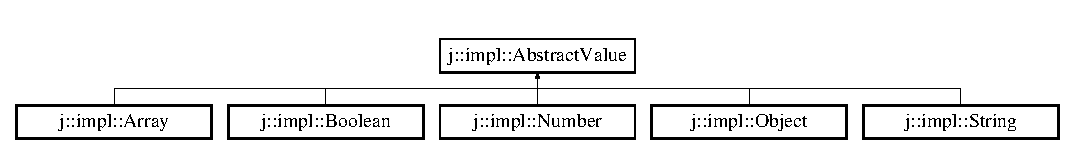
\includegraphics[height=1.635036cm]{classj_1_1impl_1_1_abstract_value}
\end{center}
\end{figure}
\subsection*{Public Member Functions}
\begin{DoxyCompactItemize}
\item 
\hyperlink{classj_1_1impl_1_1_abstract_value_afb1c372ec9e3d7bca148232bdded5f53}{Abstract\-Value} ()=default
\item 
\hyperlink{classj_1_1impl_1_1_abstract_value_abf71e5a1649fb665a962fd4233e0b2a1}{Abstract\-Value} (\hyperlink{classj_1_1impl_1_1_abstract_value}{Abstract\-Value} const \&)=delete
\item 
\hyperlink{classj_1_1impl_1_1_abstract_value}{Abstract\-Value} \& \hyperlink{classj_1_1impl_1_1_abstract_value_a17f2d4e648e692ff1990ef7094ed9c1f}{operator=} (\hyperlink{classj_1_1impl_1_1_abstract_value}{Abstract\-Value} const \&)=delete
\item 
virtual \hyperlink{classj_1_1impl_1_1_abstract_value_a6980a016e15879d8b3eed45d0f1c10bb}{$\sim$\-Abstract\-Value} ()=default
\item 
virtual bool \hyperlink{classj_1_1impl_1_1_abstract_value_ac931756f6157e90b6f824fb4ae9e6ee2}{is\-String} () const 
\item 
virtual bool \hyperlink{classj_1_1impl_1_1_abstract_value_aab7be0e32dc9a488a9597d1fad5e84f5}{is\-Number} () const 
\item 
virtual bool \hyperlink{classj_1_1impl_1_1_abstract_value_a057ddc8b2d01c7a93b998cf1fab01cdd}{is\-Boolean} () const 
\item 
virtual bool \hyperlink{classj_1_1impl_1_1_abstract_value_a62b0b78a969ba3d8ea426e46c96c2517}{is\-Object} () const 
\item 
virtual bool \hyperlink{classj_1_1impl_1_1_abstract_value_a28a367d6f2bfa668c420cc587b6daaf9}{is\-Array} () const 
\item 
std\-::string \hyperlink{classj_1_1impl_1_1_abstract_value_a64dbe0d7a865b910d5baba01d88125ae}{get\-Type\-Name} () const 
\item 
virtual \hyperlink{classj_1_1impl_1_1_string}{String} \& \hyperlink{classj_1_1impl_1_1_abstract_value_a7bbc123a13e953d51789f65d8e974aa1}{as\-String} ()
\item 
virtual \hyperlink{classj_1_1impl_1_1_string}{String} const \& \hyperlink{classj_1_1impl_1_1_abstract_value_a93ea458da59b4a9cab2cc7c359792105}{as\-String} () const 
\item 
virtual \hyperlink{classj_1_1impl_1_1_number}{Number} \& \hyperlink{classj_1_1impl_1_1_abstract_value_a12d6d18e7b575da29ba587865ba06a9c}{as\-Number} ()
\item 
virtual \hyperlink{classj_1_1impl_1_1_number}{Number} const \& \hyperlink{classj_1_1impl_1_1_abstract_value_a7b6246ea9bae83667abdbd7f58ece885}{as\-Number} () const 
\item 
virtual \hyperlink{classj_1_1impl_1_1_boolean}{Boolean} \& \hyperlink{classj_1_1impl_1_1_abstract_value_ae658e600ec0589f3a632a803fa390ad4}{as\-Boolean} ()
\item 
virtual \hyperlink{classj_1_1impl_1_1_boolean}{Boolean} const \& \hyperlink{classj_1_1impl_1_1_abstract_value_a19f38830cc9b55aa22c5eb41868b56c2}{as\-Boolean} () const 
\item 
virtual \hyperlink{classj_1_1impl_1_1_object}{Object} \& \hyperlink{classj_1_1impl_1_1_abstract_value_ab692a8f260c4f0cf45ef0b7cc13ade66}{as\-Object} ()
\item 
virtual \hyperlink{classj_1_1impl_1_1_object}{Object} const \& \hyperlink{classj_1_1impl_1_1_abstract_value_a99b098127ffda123446643bef12f574b}{as\-Object} () const 
\item 
virtual \hyperlink{classj_1_1impl_1_1_array}{Array} \& \hyperlink{classj_1_1impl_1_1_abstract_value_afd41265b99a6e385f3d3cb9679d864ab}{as\-Array} ()
\item 
virtual \hyperlink{classj_1_1impl_1_1_array}{Array} const \& \hyperlink{classj_1_1impl_1_1_abstract_value_ab9a29818092145c446517dda40e52b46}{as\-Array} () const 
\item 
virtual \hyperlink{classj_1_1impl_1_1_abstract_value}{Abstract\-Value} $\ast$ \hyperlink{classj_1_1impl_1_1_abstract_value_ac61a9aa4a4ecd3a309e8e274ac4b3dd2}{clone} () const =0
\end{DoxyCompactItemize}
\subsection*{Private Member Functions}
\begin{DoxyCompactItemize}
\item 
void \hyperlink{classj_1_1impl_1_1_abstract_value_a8844e3910ff499d9c8b96886beddbc53}{bad\-Conversion} (std\-::string const \&to) const 
\begin{DoxyCompactList}\small\item\em Fire a \hyperlink{classj_1_1_bad_conversion}{Bad\-Conversion} exception. \end{DoxyCompactList}\end{DoxyCompactItemize}


\subsection{Constructor \& Destructor Documentation}
\hypertarget{classj_1_1impl_1_1_abstract_value_afb1c372ec9e3d7bca148232bdded5f53}{\index{j\-::impl\-::\-Abstract\-Value@{j\-::impl\-::\-Abstract\-Value}!Abstract\-Value@{Abstract\-Value}}
\index{Abstract\-Value@{Abstract\-Value}!j::impl::AbstractValue@{j\-::impl\-::\-Abstract\-Value}}
\subsubsection[{Abstract\-Value}]{\setlength{\rightskip}{0pt plus 5cm}j\-::impl\-::\-Abstract\-Value\-::\-Abstract\-Value (
\begin{DoxyParamCaption}
{}
\end{DoxyParamCaption}
)\hspace{0.3cm}{\ttfamily [default]}}}\label{classj_1_1impl_1_1_abstract_value_afb1c372ec9e3d7bca148232bdded5f53}
\hypertarget{classj_1_1impl_1_1_abstract_value_abf71e5a1649fb665a962fd4233e0b2a1}{\index{j\-::impl\-::\-Abstract\-Value@{j\-::impl\-::\-Abstract\-Value}!Abstract\-Value@{Abstract\-Value}}
\index{Abstract\-Value@{Abstract\-Value}!j::impl::AbstractValue@{j\-::impl\-::\-Abstract\-Value}}
\subsubsection[{Abstract\-Value}]{\setlength{\rightskip}{0pt plus 5cm}j\-::impl\-::\-Abstract\-Value\-::\-Abstract\-Value (
\begin{DoxyParamCaption}
\item[{{\bf Abstract\-Value} const \&}]{}
\end{DoxyParamCaption}
)\hspace{0.3cm}{\ttfamily [delete]}}}\label{classj_1_1impl_1_1_abstract_value_abf71e5a1649fb665a962fd4233e0b2a1}
\hypertarget{classj_1_1impl_1_1_abstract_value_a6980a016e15879d8b3eed45d0f1c10bb}{\index{j\-::impl\-::\-Abstract\-Value@{j\-::impl\-::\-Abstract\-Value}!$\sim$\-Abstract\-Value@{$\sim$\-Abstract\-Value}}
\index{$\sim$\-Abstract\-Value@{$\sim$\-Abstract\-Value}!j::impl::AbstractValue@{j\-::impl\-::\-Abstract\-Value}}
\subsubsection[{$\sim$\-Abstract\-Value}]{\setlength{\rightskip}{0pt plus 5cm}virtual j\-::impl\-::\-Abstract\-Value\-::$\sim$\-Abstract\-Value (
\begin{DoxyParamCaption}
{}
\end{DoxyParamCaption}
)\hspace{0.3cm}{\ttfamily [virtual]}, {\ttfamily [default]}}}\label{classj_1_1impl_1_1_abstract_value_a6980a016e15879d8b3eed45d0f1c10bb}


\subsection{Member Function Documentation}
\hypertarget{classj_1_1impl_1_1_abstract_value_afd41265b99a6e385f3d3cb9679d864ab}{\index{j\-::impl\-::\-Abstract\-Value@{j\-::impl\-::\-Abstract\-Value}!as\-Array@{as\-Array}}
\index{as\-Array@{as\-Array}!j::impl::AbstractValue@{j\-::impl\-::\-Abstract\-Value}}
\subsubsection[{as\-Array}]{\setlength{\rightskip}{0pt plus 5cm}{\bf Array} \& j\-::impl\-::\-Abstract\-Value\-::as\-Array (
\begin{DoxyParamCaption}
{}
\end{DoxyParamCaption}
)\hspace{0.3cm}{\ttfamily [virtual]}}}\label{classj_1_1impl_1_1_abstract_value_afd41265b99a6e385f3d3cb9679d864ab}


Reimplemented in \hyperlink{classj_1_1impl_1_1_array_afbbbbbd781af165452dedda0a7b1ce05}{j\-::impl\-::\-Array}.

\hypertarget{classj_1_1impl_1_1_abstract_value_ab9a29818092145c446517dda40e52b46}{\index{j\-::impl\-::\-Abstract\-Value@{j\-::impl\-::\-Abstract\-Value}!as\-Array@{as\-Array}}
\index{as\-Array@{as\-Array}!j::impl::AbstractValue@{j\-::impl\-::\-Abstract\-Value}}
\subsubsection[{as\-Array}]{\setlength{\rightskip}{0pt plus 5cm}{\bf Array} const \& j\-::impl\-::\-Abstract\-Value\-::as\-Array (
\begin{DoxyParamCaption}
{}
\end{DoxyParamCaption}
) const\hspace{0.3cm}{\ttfamily [virtual]}}}\label{classj_1_1impl_1_1_abstract_value_ab9a29818092145c446517dda40e52b46}


Reimplemented in \hyperlink{classj_1_1impl_1_1_array_ab4ad4d8cba1ccf25cb209b03fb50573a}{j\-::impl\-::\-Array}.

\hypertarget{classj_1_1impl_1_1_abstract_value_ae658e600ec0589f3a632a803fa390ad4}{\index{j\-::impl\-::\-Abstract\-Value@{j\-::impl\-::\-Abstract\-Value}!as\-Boolean@{as\-Boolean}}
\index{as\-Boolean@{as\-Boolean}!j::impl::AbstractValue@{j\-::impl\-::\-Abstract\-Value}}
\subsubsection[{as\-Boolean}]{\setlength{\rightskip}{0pt plus 5cm}{\bf Boolean} \& j\-::impl\-::\-Abstract\-Value\-::as\-Boolean (
\begin{DoxyParamCaption}
{}
\end{DoxyParamCaption}
)\hspace{0.3cm}{\ttfamily [virtual]}}}\label{classj_1_1impl_1_1_abstract_value_ae658e600ec0589f3a632a803fa390ad4}


Reimplemented in \hyperlink{classj_1_1impl_1_1_boolean_a1f96b1193d7fbc41bd58fed33874f2ad}{j\-::impl\-::\-Boolean}.

\hypertarget{classj_1_1impl_1_1_abstract_value_a19f38830cc9b55aa22c5eb41868b56c2}{\index{j\-::impl\-::\-Abstract\-Value@{j\-::impl\-::\-Abstract\-Value}!as\-Boolean@{as\-Boolean}}
\index{as\-Boolean@{as\-Boolean}!j::impl::AbstractValue@{j\-::impl\-::\-Abstract\-Value}}
\subsubsection[{as\-Boolean}]{\setlength{\rightskip}{0pt plus 5cm}{\bf Boolean} const \& j\-::impl\-::\-Abstract\-Value\-::as\-Boolean (
\begin{DoxyParamCaption}
{}
\end{DoxyParamCaption}
) const\hspace{0.3cm}{\ttfamily [virtual]}}}\label{classj_1_1impl_1_1_abstract_value_a19f38830cc9b55aa22c5eb41868b56c2}


Reimplemented in \hyperlink{classj_1_1impl_1_1_boolean_a174f6cfb37900f17708bf4fb34d94aa6}{j\-::impl\-::\-Boolean}.

\hypertarget{classj_1_1impl_1_1_abstract_value_a12d6d18e7b575da29ba587865ba06a9c}{\index{j\-::impl\-::\-Abstract\-Value@{j\-::impl\-::\-Abstract\-Value}!as\-Number@{as\-Number}}
\index{as\-Number@{as\-Number}!j::impl::AbstractValue@{j\-::impl\-::\-Abstract\-Value}}
\subsubsection[{as\-Number}]{\setlength{\rightskip}{0pt plus 5cm}{\bf Number} \& j\-::impl\-::\-Abstract\-Value\-::as\-Number (
\begin{DoxyParamCaption}
{}
\end{DoxyParamCaption}
)\hspace{0.3cm}{\ttfamily [virtual]}}}\label{classj_1_1impl_1_1_abstract_value_a12d6d18e7b575da29ba587865ba06a9c}


Reimplemented in \hyperlink{classj_1_1impl_1_1_number_a86cf66c468eb3b75072bd431d8637529}{j\-::impl\-::\-Number}.

\hypertarget{classj_1_1impl_1_1_abstract_value_a7b6246ea9bae83667abdbd7f58ece885}{\index{j\-::impl\-::\-Abstract\-Value@{j\-::impl\-::\-Abstract\-Value}!as\-Number@{as\-Number}}
\index{as\-Number@{as\-Number}!j::impl::AbstractValue@{j\-::impl\-::\-Abstract\-Value}}
\subsubsection[{as\-Number}]{\setlength{\rightskip}{0pt plus 5cm}{\bf Number} const \& j\-::impl\-::\-Abstract\-Value\-::as\-Number (
\begin{DoxyParamCaption}
{}
\end{DoxyParamCaption}
) const\hspace{0.3cm}{\ttfamily [virtual]}}}\label{classj_1_1impl_1_1_abstract_value_a7b6246ea9bae83667abdbd7f58ece885}


Reimplemented in \hyperlink{classj_1_1impl_1_1_number_af72a6b872008d58ecd80547c89d9d355}{j\-::impl\-::\-Number}.

\hypertarget{classj_1_1impl_1_1_abstract_value_ab692a8f260c4f0cf45ef0b7cc13ade66}{\index{j\-::impl\-::\-Abstract\-Value@{j\-::impl\-::\-Abstract\-Value}!as\-Object@{as\-Object}}
\index{as\-Object@{as\-Object}!j::impl::AbstractValue@{j\-::impl\-::\-Abstract\-Value}}
\subsubsection[{as\-Object}]{\setlength{\rightskip}{0pt plus 5cm}{\bf Object} \& j\-::impl\-::\-Abstract\-Value\-::as\-Object (
\begin{DoxyParamCaption}
{}
\end{DoxyParamCaption}
)\hspace{0.3cm}{\ttfamily [virtual]}}}\label{classj_1_1impl_1_1_abstract_value_ab692a8f260c4f0cf45ef0b7cc13ade66}


Reimplemented in \hyperlink{classj_1_1impl_1_1_object_aad1449adafdd83c980a03061ebf197c0}{j\-::impl\-::\-Object}.

\hypertarget{classj_1_1impl_1_1_abstract_value_a99b098127ffda123446643bef12f574b}{\index{j\-::impl\-::\-Abstract\-Value@{j\-::impl\-::\-Abstract\-Value}!as\-Object@{as\-Object}}
\index{as\-Object@{as\-Object}!j::impl::AbstractValue@{j\-::impl\-::\-Abstract\-Value}}
\subsubsection[{as\-Object}]{\setlength{\rightskip}{0pt plus 5cm}{\bf Object} const \& j\-::impl\-::\-Abstract\-Value\-::as\-Object (
\begin{DoxyParamCaption}
{}
\end{DoxyParamCaption}
) const\hspace{0.3cm}{\ttfamily [virtual]}}}\label{classj_1_1impl_1_1_abstract_value_a99b098127ffda123446643bef12f574b}


Reimplemented in \hyperlink{classj_1_1impl_1_1_object_a931f6aabe40406eb81106d0ec45ac1bd}{j\-::impl\-::\-Object}.

\hypertarget{classj_1_1impl_1_1_abstract_value_a7bbc123a13e953d51789f65d8e974aa1}{\index{j\-::impl\-::\-Abstract\-Value@{j\-::impl\-::\-Abstract\-Value}!as\-String@{as\-String}}
\index{as\-String@{as\-String}!j::impl::AbstractValue@{j\-::impl\-::\-Abstract\-Value}}
\subsubsection[{as\-String}]{\setlength{\rightskip}{0pt plus 5cm}{\bf String} \& j\-::impl\-::\-Abstract\-Value\-::as\-String (
\begin{DoxyParamCaption}
{}
\end{DoxyParamCaption}
)\hspace{0.3cm}{\ttfamily [virtual]}}}\label{classj_1_1impl_1_1_abstract_value_a7bbc123a13e953d51789f65d8e974aa1}


Reimplemented in \hyperlink{classj_1_1impl_1_1_string_a0a9ce87a737e81d5a035fa756d7ecd60}{j\-::impl\-::\-String}.

\hypertarget{classj_1_1impl_1_1_abstract_value_a93ea458da59b4a9cab2cc7c359792105}{\index{j\-::impl\-::\-Abstract\-Value@{j\-::impl\-::\-Abstract\-Value}!as\-String@{as\-String}}
\index{as\-String@{as\-String}!j::impl::AbstractValue@{j\-::impl\-::\-Abstract\-Value}}
\subsubsection[{as\-String}]{\setlength{\rightskip}{0pt plus 5cm}{\bf String} const \& j\-::impl\-::\-Abstract\-Value\-::as\-String (
\begin{DoxyParamCaption}
{}
\end{DoxyParamCaption}
) const\hspace{0.3cm}{\ttfamily [virtual]}}}\label{classj_1_1impl_1_1_abstract_value_a93ea458da59b4a9cab2cc7c359792105}


Reimplemented in \hyperlink{classj_1_1impl_1_1_string_aaa33cceb60b66372afe727dba5621315}{j\-::impl\-::\-String}.

\hypertarget{classj_1_1impl_1_1_abstract_value_a8844e3910ff499d9c8b96886beddbc53}{\index{j\-::impl\-::\-Abstract\-Value@{j\-::impl\-::\-Abstract\-Value}!bad\-Conversion@{bad\-Conversion}}
\index{bad\-Conversion@{bad\-Conversion}!j::impl::AbstractValue@{j\-::impl\-::\-Abstract\-Value}}
\subsubsection[{bad\-Conversion}]{\setlength{\rightskip}{0pt plus 5cm}void j\-::impl\-::\-Abstract\-Value\-::bad\-Conversion (
\begin{DoxyParamCaption}
\item[{std\-::string const \&}]{to}
\end{DoxyParamCaption}
) const\hspace{0.3cm}{\ttfamily [private]}}}\label{classj_1_1impl_1_1_abstract_value_a8844e3910ff499d9c8b96886beddbc53}


Fire a \hyperlink{classj_1_1_bad_conversion}{Bad\-Conversion} exception. 


\begin{DoxyParams}{Parameters}
{\em to} & another type\\
\hline
\end{DoxyParams}
\begin{DoxyReturn}{Returns}
never returns 
\end{DoxyReturn}
\hypertarget{classj_1_1impl_1_1_abstract_value_ac61a9aa4a4ecd3a309e8e274ac4b3dd2}{\index{j\-::impl\-::\-Abstract\-Value@{j\-::impl\-::\-Abstract\-Value}!clone@{clone}}
\index{clone@{clone}!j::impl::AbstractValue@{j\-::impl\-::\-Abstract\-Value}}
\subsubsection[{clone}]{\setlength{\rightskip}{0pt plus 5cm}virtual {\bf Abstract\-Value}$\ast$ j\-::impl\-::\-Abstract\-Value\-::clone (
\begin{DoxyParamCaption}
{}
\end{DoxyParamCaption}
) const\hspace{0.3cm}{\ttfamily [pure virtual]}}}\label{classj_1_1impl_1_1_abstract_value_ac61a9aa4a4ecd3a309e8e274ac4b3dd2}


Implemented in \hyperlink{classj_1_1impl_1_1_array_a94e77caeb46bfcfbbf138fa75076235f}{j\-::impl\-::\-Array}, \hyperlink{classj_1_1impl_1_1_object_a7485852de6358152ec02e2e4023e3600}{j\-::impl\-::\-Object}, \hyperlink{classj_1_1impl_1_1_boolean_a299b417212ed86a52b08e2bdbd6921f0}{j\-::impl\-::\-Boolean}, \hyperlink{classj_1_1impl_1_1_number_a4b48134b69e2fa6397477b1bd8334f68}{j\-::impl\-::\-Number}, and \hyperlink{classj_1_1impl_1_1_string_ac449f19ca6504c13249db0c035444179}{j\-::impl\-::\-String}.

\hypertarget{classj_1_1impl_1_1_abstract_value_a64dbe0d7a865b910d5baba01d88125ae}{\index{j\-::impl\-::\-Abstract\-Value@{j\-::impl\-::\-Abstract\-Value}!get\-Type\-Name@{get\-Type\-Name}}
\index{get\-Type\-Name@{get\-Type\-Name}!j::impl::AbstractValue@{j\-::impl\-::\-Abstract\-Value}}
\subsubsection[{get\-Type\-Name}]{\setlength{\rightskip}{0pt plus 5cm}std\-::string j\-::impl\-::\-Abstract\-Value\-::get\-Type\-Name (
\begin{DoxyParamCaption}
{}
\end{DoxyParamCaption}
) const}}\label{classj_1_1impl_1_1_abstract_value_a64dbe0d7a865b910d5baba01d88125ae}
\hypertarget{classj_1_1impl_1_1_abstract_value_a28a367d6f2bfa668c420cc587b6daaf9}{\index{j\-::impl\-::\-Abstract\-Value@{j\-::impl\-::\-Abstract\-Value}!is\-Array@{is\-Array}}
\index{is\-Array@{is\-Array}!j::impl::AbstractValue@{j\-::impl\-::\-Abstract\-Value}}
\subsubsection[{is\-Array}]{\setlength{\rightskip}{0pt plus 5cm}bool j\-::impl\-::\-Abstract\-Value\-::is\-Array (
\begin{DoxyParamCaption}
{}
\end{DoxyParamCaption}
) const\hspace{0.3cm}{\ttfamily [virtual]}}}\label{classj_1_1impl_1_1_abstract_value_a28a367d6f2bfa668c420cc587b6daaf9}


Reimplemented in \hyperlink{classj_1_1impl_1_1_array_af859820f212b3bb3bb93c6bc98e756c1}{j\-::impl\-::\-Array}.

\hypertarget{classj_1_1impl_1_1_abstract_value_a057ddc8b2d01c7a93b998cf1fab01cdd}{\index{j\-::impl\-::\-Abstract\-Value@{j\-::impl\-::\-Abstract\-Value}!is\-Boolean@{is\-Boolean}}
\index{is\-Boolean@{is\-Boolean}!j::impl::AbstractValue@{j\-::impl\-::\-Abstract\-Value}}
\subsubsection[{is\-Boolean}]{\setlength{\rightskip}{0pt plus 5cm}bool j\-::impl\-::\-Abstract\-Value\-::is\-Boolean (
\begin{DoxyParamCaption}
{}
\end{DoxyParamCaption}
) const\hspace{0.3cm}{\ttfamily [virtual]}}}\label{classj_1_1impl_1_1_abstract_value_a057ddc8b2d01c7a93b998cf1fab01cdd}


Reimplemented in \hyperlink{classj_1_1impl_1_1_boolean_ab27b415c6e0d08400ca53b5c5bcde6d2}{j\-::impl\-::\-Boolean}.

\hypertarget{classj_1_1impl_1_1_abstract_value_aab7be0e32dc9a488a9597d1fad5e84f5}{\index{j\-::impl\-::\-Abstract\-Value@{j\-::impl\-::\-Abstract\-Value}!is\-Number@{is\-Number}}
\index{is\-Number@{is\-Number}!j::impl::AbstractValue@{j\-::impl\-::\-Abstract\-Value}}
\subsubsection[{is\-Number}]{\setlength{\rightskip}{0pt plus 5cm}bool j\-::impl\-::\-Abstract\-Value\-::is\-Number (
\begin{DoxyParamCaption}
{}
\end{DoxyParamCaption}
) const\hspace{0.3cm}{\ttfamily [virtual]}}}\label{classj_1_1impl_1_1_abstract_value_aab7be0e32dc9a488a9597d1fad5e84f5}


Reimplemented in \hyperlink{classj_1_1impl_1_1_number_a90888fbf7797a69fae21d3f6ad68fc84}{j\-::impl\-::\-Number}.

\hypertarget{classj_1_1impl_1_1_abstract_value_a62b0b78a969ba3d8ea426e46c96c2517}{\index{j\-::impl\-::\-Abstract\-Value@{j\-::impl\-::\-Abstract\-Value}!is\-Object@{is\-Object}}
\index{is\-Object@{is\-Object}!j::impl::AbstractValue@{j\-::impl\-::\-Abstract\-Value}}
\subsubsection[{is\-Object}]{\setlength{\rightskip}{0pt plus 5cm}bool j\-::impl\-::\-Abstract\-Value\-::is\-Object (
\begin{DoxyParamCaption}
{}
\end{DoxyParamCaption}
) const\hspace{0.3cm}{\ttfamily [virtual]}}}\label{classj_1_1impl_1_1_abstract_value_a62b0b78a969ba3d8ea426e46c96c2517}


Reimplemented in \hyperlink{classj_1_1impl_1_1_object_a1a4c68884081496e04f4a84684980871}{j\-::impl\-::\-Object}.

\hypertarget{classj_1_1impl_1_1_abstract_value_ac931756f6157e90b6f824fb4ae9e6ee2}{\index{j\-::impl\-::\-Abstract\-Value@{j\-::impl\-::\-Abstract\-Value}!is\-String@{is\-String}}
\index{is\-String@{is\-String}!j::impl::AbstractValue@{j\-::impl\-::\-Abstract\-Value}}
\subsubsection[{is\-String}]{\setlength{\rightskip}{0pt plus 5cm}bool j\-::impl\-::\-Abstract\-Value\-::is\-String (
\begin{DoxyParamCaption}
{}
\end{DoxyParamCaption}
) const\hspace{0.3cm}{\ttfamily [virtual]}}}\label{classj_1_1impl_1_1_abstract_value_ac931756f6157e90b6f824fb4ae9e6ee2}


Reimplemented in \hyperlink{classj_1_1impl_1_1_string_a6ca9214f2d17ebfd0375b4c24e233c89}{j\-::impl\-::\-String}.

\hypertarget{classj_1_1impl_1_1_abstract_value_a17f2d4e648e692ff1990ef7094ed9c1f}{\index{j\-::impl\-::\-Abstract\-Value@{j\-::impl\-::\-Abstract\-Value}!operator=@{operator=}}
\index{operator=@{operator=}!j::impl::AbstractValue@{j\-::impl\-::\-Abstract\-Value}}
\subsubsection[{operator=}]{\setlength{\rightskip}{0pt plus 5cm}{\bf Abstract\-Value}\& j\-::impl\-::\-Abstract\-Value\-::operator= (
\begin{DoxyParamCaption}
\item[{{\bf Abstract\-Value} const \&}]{}
\end{DoxyParamCaption}
)\hspace{0.3cm}{\ttfamily [delete]}}}\label{classj_1_1impl_1_1_abstract_value_a17f2d4e648e692ff1990ef7094ed9c1f}


The documentation for this class was generated from the following files\-:\begin{DoxyCompactItemize}
\item 
/home/jbesson/myfiles/cpp/svprog/partie1/src/\-J\-S\-O\-N/\hyperlink{_j_s_o_n_impl_8hpp}{J\-S\-O\-N\-Impl.\-hpp}\item 
/home/jbesson/myfiles/cpp/svprog/partie1/src/\-J\-S\-O\-N/\hyperlink{_j_s_o_n_impl_8cpp}{J\-S\-O\-N\-Impl.\-cpp}\end{DoxyCompactItemize}

\hypertarget{class_application}{\section{Application Class Reference}
\label{class_application}\index{Application@{Application}}
}


Abstract class managing the core of the program.  




{\ttfamily \#include $<$Application.\-hpp$>$}

Inheritance diagram for Application\-:\begin{figure}[H]
\begin{center}
\leavevmode
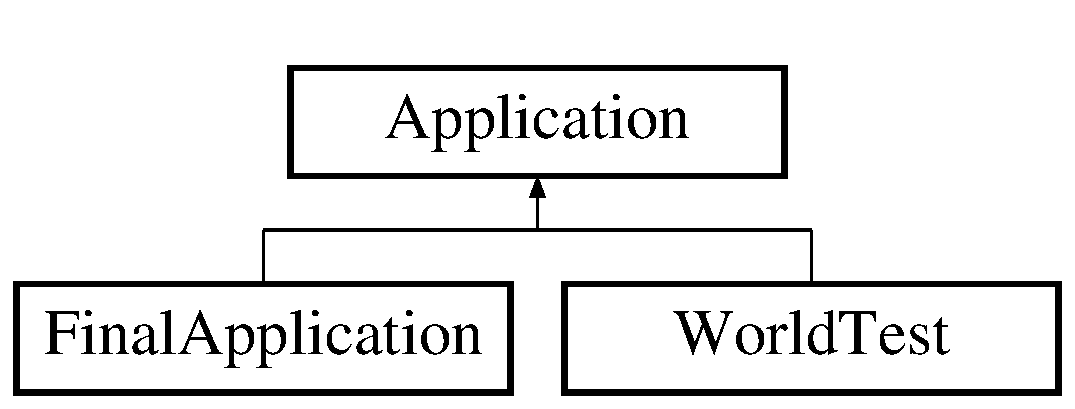
\includegraphics[height=2.000000cm]{class_application}
\end{center}
\end{figure}
\subsection*{Public Member Functions}
\begin{DoxyCompactItemize}
\item 
\hyperlink{class_application_a571b19044041fe7b63f0da45dc56532e}{Application} (int argc, char const $\ast$$\ast$argv)
\begin{DoxyCompactList}\small\item\em Constructor. \end{DoxyCompactList}\item 
\hyperlink{class_application_a045b831793669ac925c635dcb4786087}{Application} (\hyperlink{class_application}{Application} const \&)=delete
\begin{DoxyCompactList}\small\item\em Forbid copy. \end{DoxyCompactList}\item 
\hyperlink{class_application}{Application} \& \hyperlink{class_application_a1fee125c91f0e7c1fcb7a7fd4318c74e}{operator=} (\hyperlink{class_application}{Application} const \&)=delete
\item 
virtual \hyperlink{class_application_a748bca84fefb9c12661cfaa2f623748d}{$\sim$\-Application} ()
\begin{DoxyCompactList}\small\item\em Destructor. \end{DoxyCompactList}\item 
void \hyperlink{class_application_a68965449404743bf1add056784d6cf81}{run} ()
\begin{DoxyCompactList}\small\item\em Run the application. \end{DoxyCompactList}\item 
Env \& \hyperlink{class_application_a66c2e8b7340252006680158876db46e1}{get\-Env} ()
\begin{DoxyCompactList}\small\item\em Get access to the execution environment of the application (the env) \end{DoxyCompactList}\item 
Env const \& \hyperlink{class_application_a88fc89d94da74af06091464e1dfe4a8f}{get\-Env} () const 
\item 
\hyperlink{classj_1_1_value}{j\-::\-Value} \& \hyperlink{class_application_a40ada3828cedc56606182850eb1ea267}{get\-Config} ()
\begin{DoxyCompactList}\small\item\em Get the bee tracker helper. \end{DoxyCompactList}\item 
\hyperlink{classj_1_1_value}{j\-::\-Value} const \& \hyperlink{class_application_a976052594bde1619931c0942967b9a92}{get\-Config} () const 
\item 
sf\-::\-Font const \& \hyperlink{class_application_af9ef0f6c5a9fde1cf31d7fad3e3176d6}{get\-Font} () const 
\begin{DoxyCompactList}\small\item\em Get the app's font. \end{DoxyCompactList}\item 
sf\-::\-Texture \& \hyperlink{class_application_a18f35a0326625f9818003dc7353d4208}{get\-Texture} (std\-::string const \&name)
\begin{DoxyCompactList}\small\item\em Get a texture. \end{DoxyCompactList}\item 
std\-::string \hyperlink{class_application_aefb5a8a34ddfbffd38481010a71a1a4c}{get\-Res\-Path} () const 
\begin{DoxyCompactList}\small\item\em Get the path to the resource folder. \end{DoxyCompactList}\item 
\hyperlink{class_vec2d}{Vec2d} \hyperlink{class_application_ad55493fb479ede7b4c613c6d1c204180}{get\-World\-Size} () const 
\begin{DoxyCompactList}\small\item\em Read the world size from the config manager. \end{DoxyCompactList}\item 
\hyperlink{class_vec2d}{Vec2d} \hyperlink{class_application_a6bc4c1a004c1d3dd23afae420cd72978}{get\-Centre} () const 
\begin{DoxyCompactList}\small\item\em Compute the centre of the world area (in local coordinates) \end{DoxyCompactList}\item 
\hyperlink{class_vec2d}{Vec2d} \hyperlink{class_application_a7d49c36d1dff894f7d5533c614d9cf36}{get\-Cursor\-Position\-In\-View} () const 
\begin{DoxyCompactList}\small\item\em Get the cursor position in the view coordinates (i.\-e. pixel coordinates) \end{DoxyCompactList}\end{DoxyCompactItemize}
\subsection*{Private Types}
\begin{DoxyCompactItemize}
\item 
using \hyperlink{class_application_a5d2ae97c527f0ba88c259f2fdcecbb9b}{Texture\-Pool} = std\-::map$<$ std\-::string, sf\-::\-Texture $\ast$ $>$
\end{DoxyCompactItemize}
\subsection*{Private Member Functions}
\begin{DoxyCompactItemize}
\item 
virtual void \hyperlink{class_application_af48ce2f324313699257c164dddb3b920}{on\-Run} ()
\begin{DoxyCompactList}\small\item\em Add a graph to the stats manager and update G\-U\-I. \end{DoxyCompactList}\item 
virtual void \hyperlink{class_application_a811e40a46923de963bbc87d54097ed54}{on\-Simulation\-Start} ()
\begin{DoxyCompactList}\small\item\em Called when the simulation is (re)started, but not when importing data. \end{DoxyCompactList}\item 
virtual void \hyperlink{class_application_ae6ea28bafe249f7005aa143f36651342}{on\-Event} (sf\-::\-Event event, sf\-::\-Render\-Window \&window)
\begin{DoxyCompactList}\small\item\em Subclass can override this method to handle events. \end{DoxyCompactList}\item 
virtual void \hyperlink{class_application_adfc65fcc3dda8aab7483d01f8b2b1e48}{on\-Update} (sf\-::\-Time dt)
\begin{DoxyCompactList}\small\item\em Subclass can override this method to update their data. \end{DoxyCompactList}\item 
virtual void \hyperlink{class_application_ac35bfbd486eb47fdd2b5d731962c6724}{on\-Draw} (sf\-::\-Render\-Target \&target)
\begin{DoxyCompactList}\small\item\em Subclass can override this method to draw their data in the simulation view. \end{DoxyCompactList}\item 
void \hyperlink{class_application_a8634280ed0a49eb67c2698a076f51a36}{create\-Window} (\hyperlink{class_vec2d}{Vec2d} const \&size)
\begin{DoxyCompactList}\small\item\em Create the window. \end{DoxyCompactList}\item 
void \hyperlink{class_application_a243bb0cf151bdaa9bc16e06498964cf6}{create\-Views} ()
\begin{DoxyCompactList}\small\item\em Create the simulation and stats views. \end{DoxyCompactList}\item 
void \hyperlink{class_application_aaac48a5982dd7c72f727f917347b07aa}{handle\-Event} (sf\-::\-Event event, sf\-::\-Render\-Window \&window)
\begin{DoxyCompactList}\small\item\em Do the logic for a given event. \end{DoxyCompactList}\item 
void \hyperlink{class_application_af3a3bba5fac5920c26ddb4ccd3ae69fa}{render} (sf\-::\-Drawable const \&simulation\-Background, sf\-::\-Drawable const \&stats\-Background)
\begin{DoxyCompactList}\small\item\em Render the G\-U\-I, Simulation and Stats. \end{DoxyCompactList}\item 
Stats \& \hyperlink{class_application_a9d9d5670dfd9ca54b4c39bb9b870d106}{get\-Stats} ()
\begin{DoxyCompactList}\small\item\em Get access to the stats manager. \end{DoxyCompactList}\item 
void \hyperlink{class_application_af03097cece8f7dbbe744bd7a242af033}{toggle\-Pause} ()
\begin{DoxyCompactList}\small\item\em Toggle pause. \end{DoxyCompactList}\item 
void \hyperlink{class_application_aed88c8943b8df942461e99c226d5bee2}{save\-Config} () const 
\begin{DoxyCompactList}\small\item\em Save the current configuration. \end{DoxyCompactList}\item 
void \hyperlink{class_application_aeecb0f55acec51532399693799d19fe7}{zoom\-View\-At} (sf\-::\-Vector2i const \&pixel, float zoom\-Factor)
\begin{DoxyCompactList}\small\item\em Zoom the simulation view on the given pixel. \end{DoxyCompactList}\item 
void \hyperlink{class_application_a3089c41134287645292eeb587f917f89}{drag\-View} (sf\-::\-Vector2i const \&src\-Pixel, sf\-::\-Vector2i const \&dest\-Pixel)
\begin{DoxyCompactList}\small\item\em Drag the view by the given offset (i.\-e. src to dest) \end{DoxyCompactList}\item 
void \hyperlink{class_application_a5d6a3cc615a2b345167b337c451c8d7e}{update\-Simulation\-View} ()
\begin{DoxyCompactList}\small\item\em Center the simulation view on the tracked bee, if selection is active. \end{DoxyCompactList}\end{DoxyCompactItemize}
\subsection*{Private Attributes}
\begin{DoxyCompactItemize}
\item 
std\-::string const \hyperlink{class_application_a4dfc28cc57cbf7099a9fb307f1bddb66}{m\-App\-Directory}
\begin{DoxyCompactList}\small\item\em Path to the executable's directory. \end{DoxyCompactList}\item 
std\-::string const \hyperlink{class_application_a47b102eeb6056257fad1b1073c62cd0e}{m\-Cfg\-File}
\begin{DoxyCompactList}\small\item\em Relative path to the C\-F\-G. \end{DoxyCompactList}\item 
\hyperlink{classj_1_1_value}{j\-::\-Value} \hyperlink{class_application_a7d54750ac09a1bc7e4d72944bb52e393}{m\-Config}
\begin{DoxyCompactList}\small\item\em \hyperlink{class_application}{Application} configuration. \end{DoxyCompactList}\item 
Env $\ast$ \hyperlink{class_application_a17edefa78adf28e93132ce3d9af8aad5}{m\-Env}
\begin{DoxyCompactList}\small\item\em Simulated environment. \end{DoxyCompactList}\item 
sf\-::\-Font \hyperlink{class_application_a697d840b0ef9b447a9463996d5963e10}{m\-Font}
\begin{DoxyCompactList}\small\item\em A font. \end{DoxyCompactList}\item 
sf\-::\-Render\-Window \hyperlink{class_application_acde37e91150ea3a16e9e4849e08c7784}{m\-Render\-Window}
\begin{DoxyCompactList}\small\item\em S\-F\-M\-L window / render target. \end{DoxyCompactList}\item 
sf\-::\-View \hyperlink{class_application_a74a68526ce8ee51762f6d3313355b918}{m\-Simulation\-View}
\begin{DoxyCompactList}\small\item\em View for simulation area. \end{DoxyCompactList}\item 
Stats $\ast$ \hyperlink{class_application_a58c0745f95a42c636a1b914dac2e1ae6}{m\-Stats}
\begin{DoxyCompactList}\small\item\em Statistic manager. \end{DoxyCompactList}\item 
sf\-::\-View \hyperlink{class_application_a823c6ca5d9d397554b397810c940355a}{m\-Stats\-View}
\begin{DoxyCompactList}\small\item\em View for the stats area. \end{DoxyCompactList}\item 
\hyperlink{class_application_a5d2ae97c527f0ba88c259f2fdcecbb9b}{Texture\-Pool} \hyperlink{class_application_adee1221b74e94ac0fe94b3c99f52e03a}{m\-Textures}
\begin{DoxyCompactList}\small\item\em Pool of textures. \end{DoxyCompactList}\item 
sf\-::\-Texture \hyperlink{class_application_a79cda06cffa4e262a9c4ec066726831d}{m\-Default\-Texture}
\begin{DoxyCompactList}\small\item\em Default, white texture. \end{DoxyCompactList}\item 
bool \hyperlink{class_application_a29fd44db5b424d85f0fd35eee2494d1e}{m\-Paused}
\begin{DoxyCompactList}\small\item\em Tells if the application is in pause or not. \end{DoxyCompactList}\item 
bool \hyperlink{class_application_a2e3fd7543cf6e9a1da9940b60c512456}{m\-Is\-Resetting}
\item 
bool \hyperlink{class_application_a2d1510e1159955e12660faf4ad1230a0}{m\-Is\-Dragging}
\begin{DoxyCompactList}\small\item\em Tells whether or not the user is dragging the view. \end{DoxyCompactList}\item 
sf\-::\-Vector2i \hyperlink{class_application_a26c9135cd4290fbd7619f58f1a0c602b}{m\-Last\-Cursor\-Position}
\begin{DoxyCompactList}\small\item\em For handling dragging logic. \end{DoxyCompactList}\end{DoxyCompactItemize}


\subsection{Detailed Description}
Abstract class managing the core of the program. 

Subclass can optionally re-\/implement \hyperlink{class_application_ae6ea28bafe249f7005aa143f36651342}{on\-Event()}, \hyperlink{class_application_adfc65fcc3dda8aab7483d01f8b2b1e48}{on\-Update()} and \hyperlink{class_application_ac35bfbd486eb47fdd2b5d731962c6724}{on\-Draw()}.

The Env class handles the drawing and update of the system.

Note that {\ttfamily simulation} and {\ttfamily world} usually mean the same thing here. 

\subsection{Member Typedef Documentation}
\hypertarget{class_application_a5d2ae97c527f0ba88c259f2fdcecbb9b}{\index{Application@{Application}!Texture\-Pool@{Texture\-Pool}}
\index{Texture\-Pool@{Texture\-Pool}!Application@{Application}}
\subsubsection[{Texture\-Pool}]{\setlength{\rightskip}{0pt plus 5cm}using {\bf Application\-::\-Texture\-Pool} =  std\-::map$<$std\-::string, sf\-::\-Texture$\ast$$>$\hspace{0.3cm}{\ttfamily [private]}}}\label{class_application_a5d2ae97c527f0ba88c259f2fdcecbb9b}


\subsection{Constructor \& Destructor Documentation}
\hypertarget{class_application_a571b19044041fe7b63f0da45dc56532e}{\index{Application@{Application}!Application@{Application}}
\index{Application@{Application}!Application@{Application}}
\subsubsection[{Application}]{\setlength{\rightskip}{0pt plus 5cm}Application\-::\-Application (
\begin{DoxyParamCaption}
\item[{int}]{argc, }
\item[{char const $\ast$$\ast$}]{argv}
\end{DoxyParamCaption}
)}}\label{class_application_a571b19044041fe7b63f0da45dc56532e}


Constructor. 


\begin{DoxyParams}{Parameters}
{\em argc} & argument count \\
\hline
{\em argv} & launch arguments \\
\hline
\end{DoxyParams}
\hypertarget{class_application_a045b831793669ac925c635dcb4786087}{\index{Application@{Application}!Application@{Application}}
\index{Application@{Application}!Application@{Application}}
\subsubsection[{Application}]{\setlength{\rightskip}{0pt plus 5cm}Application\-::\-Application (
\begin{DoxyParamCaption}
\item[{{\bf Application} const \&}]{}
\end{DoxyParamCaption}
)\hspace{0.3cm}{\ttfamily [delete]}}}\label{class_application_a045b831793669ac925c635dcb4786087}


Forbid copy. 

\hypertarget{class_application_a748bca84fefb9c12661cfaa2f623748d}{\index{Application@{Application}!$\sim$\-Application@{$\sim$\-Application}}
\index{$\sim$\-Application@{$\sim$\-Application}!Application@{Application}}
\subsubsection[{$\sim$\-Application}]{\setlength{\rightskip}{0pt plus 5cm}Application\-::$\sim$\-Application (
\begin{DoxyParamCaption}
{}
\end{DoxyParamCaption}
)\hspace{0.3cm}{\ttfamily [virtual]}}}\label{class_application_a748bca84fefb9c12661cfaa2f623748d}


Destructor. 



\subsection{Member Function Documentation}
\hypertarget{class_application_a243bb0cf151bdaa9bc16e06498964cf6}{\index{Application@{Application}!create\-Views@{create\-Views}}
\index{create\-Views@{create\-Views}!Application@{Application}}
\subsubsection[{create\-Views}]{\setlength{\rightskip}{0pt plus 5cm}void Application\-::create\-Views (
\begin{DoxyParamCaption}
{}
\end{DoxyParamCaption}
)\hspace{0.3cm}{\ttfamily [private]}}}\label{class_application_a243bb0cf151bdaa9bc16e06498964cf6}


Create the simulation and stats views. 

\hypertarget{class_application_a8634280ed0a49eb67c2698a076f51a36}{\index{Application@{Application}!create\-Window@{create\-Window}}
\index{create\-Window@{create\-Window}!Application@{Application}}
\subsubsection[{create\-Window}]{\setlength{\rightskip}{0pt plus 5cm}void Application\-::create\-Window (
\begin{DoxyParamCaption}
\item[{{\bf Vec2d} const \&}]{size}
\end{DoxyParamCaption}
)\hspace{0.3cm}{\ttfamily [private]}}}\label{class_application_a8634280ed0a49eb67c2698a076f51a36}


Create the window. 

\hypertarget{class_application_a3089c41134287645292eeb587f917f89}{\index{Application@{Application}!drag\-View@{drag\-View}}
\index{drag\-View@{drag\-View}!Application@{Application}}
\subsubsection[{drag\-View}]{\setlength{\rightskip}{0pt plus 5cm}void Application\-::drag\-View (
\begin{DoxyParamCaption}
\item[{sf\-::\-Vector2i const \&}]{src\-Pixel, }
\item[{sf\-::\-Vector2i const \&}]{dest\-Pixel}
\end{DoxyParamCaption}
)\hspace{0.3cm}{\ttfamily [private]}}}\label{class_application_a3089c41134287645292eeb587f917f89}


Drag the view by the given offset (i.\-e. src to dest) 

\hypertarget{class_application_a6bc4c1a004c1d3dd23afae420cd72978}{\index{Application@{Application}!get\-Centre@{get\-Centre}}
\index{get\-Centre@{get\-Centre}!Application@{Application}}
\subsubsection[{get\-Centre}]{\setlength{\rightskip}{0pt plus 5cm}{\bf Vec2d} Application\-::get\-Centre (
\begin{DoxyParamCaption}
{}
\end{DoxyParamCaption}
) const}}\label{class_application_a6bc4c1a004c1d3dd23afae420cd72978}


Compute the centre of the world area (in local coordinates) 

\begin{DoxyReturn}{Returns}
the centre of the app 
\end{DoxyReturn}
\hypertarget{class_application_a40ada3828cedc56606182850eb1ea267}{\index{Application@{Application}!get\-Config@{get\-Config}}
\index{get\-Config@{get\-Config}!Application@{Application}}
\subsubsection[{get\-Config}]{\setlength{\rightskip}{0pt plus 5cm}{\bf j\-::\-Value} \& Application\-::get\-Config (
\begin{DoxyParamCaption}
{}
\end{DoxyParamCaption}
)}}\label{class_application_a40ada3828cedc56606182850eb1ea267}


Get the bee tracker helper. 

\begin{DoxyReturn}{Returns}
the app's bee tracker
\end{DoxyReturn}
Get access to the application's configuration

\begin{DoxyReturn}{Returns}
the app's config 
\end{DoxyReturn}
\hypertarget{class_application_a976052594bde1619931c0942967b9a92}{\index{Application@{Application}!get\-Config@{get\-Config}}
\index{get\-Config@{get\-Config}!Application@{Application}}
\subsubsection[{get\-Config}]{\setlength{\rightskip}{0pt plus 5cm}{\bf j\-::\-Value} const \& Application\-::get\-Config (
\begin{DoxyParamCaption}
{}
\end{DoxyParamCaption}
) const}}\label{class_application_a976052594bde1619931c0942967b9a92}
\hypertarget{class_application_a7d49c36d1dff894f7d5533c614d9cf36}{\index{Application@{Application}!get\-Cursor\-Position\-In\-View@{get\-Cursor\-Position\-In\-View}}
\index{get\-Cursor\-Position\-In\-View@{get\-Cursor\-Position\-In\-View}!Application@{Application}}
\subsubsection[{get\-Cursor\-Position\-In\-View}]{\setlength{\rightskip}{0pt plus 5cm}{\bf Vec2d} Application\-::get\-Cursor\-Position\-In\-View (
\begin{DoxyParamCaption}
{}
\end{DoxyParamCaption}
) const}}\label{class_application_a7d49c36d1dff894f7d5533c614d9cf36}


Get the cursor position in the view coordinates (i.\-e. pixel coordinates) 

\begin{DoxyReturn}{Returns}
The cursor position converted in the view coordinates 
\end{DoxyReturn}
\hypertarget{class_application_a66c2e8b7340252006680158876db46e1}{\index{Application@{Application}!get\-Env@{get\-Env}}
\index{get\-Env@{get\-Env}!Application@{Application}}
\subsubsection[{get\-Env}]{\setlength{\rightskip}{0pt plus 5cm}Env \& Application\-::get\-Env (
\begin{DoxyParamCaption}
{}
\end{DoxyParamCaption}
)}}\label{class_application_a66c2e8b7340252006680158876db46e1}


Get access to the execution environment of the application (the env) 

\begin{DoxyNote}{Note}
This breaks the encapsulation but simplify everything!
\end{DoxyNote}
\begin{DoxyReturn}{Returns}
the app's env 
\end{DoxyReturn}
\hypertarget{class_application_a88fc89d94da74af06091464e1dfe4a8f}{\index{Application@{Application}!get\-Env@{get\-Env}}
\index{get\-Env@{get\-Env}!Application@{Application}}
\subsubsection[{get\-Env}]{\setlength{\rightskip}{0pt plus 5cm}Env const \& Application\-::get\-Env (
\begin{DoxyParamCaption}
{}
\end{DoxyParamCaption}
) const}}\label{class_application_a88fc89d94da74af06091464e1dfe4a8f}
\hypertarget{class_application_af9ef0f6c5a9fde1cf31d7fad3e3176d6}{\index{Application@{Application}!get\-Font@{get\-Font}}
\index{get\-Font@{get\-Font}!Application@{Application}}
\subsubsection[{get\-Font}]{\setlength{\rightskip}{0pt plus 5cm}sf\-::\-Font const \& Application\-::get\-Font (
\begin{DoxyParamCaption}
{}
\end{DoxyParamCaption}
) const}}\label{class_application_af9ef0f6c5a9fde1cf31d7fad3e3176d6}


Get the app's font. 

\begin{DoxyReturn}{Returns}
a font 
\end{DoxyReturn}
\hypertarget{class_application_aefb5a8a34ddfbffd38481010a71a1a4c}{\index{Application@{Application}!get\-Res\-Path@{get\-Res\-Path}}
\index{get\-Res\-Path@{get\-Res\-Path}!Application@{Application}}
\subsubsection[{get\-Res\-Path}]{\setlength{\rightskip}{0pt plus 5cm}std\-::string Application\-::get\-Res\-Path (
\begin{DoxyParamCaption}
{}
\end{DoxyParamCaption}
) const}}\label{class_application_aefb5a8a34ddfbffd38481010a71a1a4c}


Get the path to the resource folder. 

\hypertarget{class_application_a9d9d5670dfd9ca54b4c39bb9b870d106}{\index{Application@{Application}!get\-Stats@{get\-Stats}}
\index{get\-Stats@{get\-Stats}!Application@{Application}}
\subsubsection[{get\-Stats}]{\setlength{\rightskip}{0pt plus 5cm}Stats \& Application\-::get\-Stats (
\begin{DoxyParamCaption}
{}
\end{DoxyParamCaption}
)\hspace{0.3cm}{\ttfamily [private]}}}\label{class_application_a9d9d5670dfd9ca54b4c39bb9b870d106}


Get access to the stats manager. 

\begin{DoxyReturn}{Returns}
the application statistic manager 
\end{DoxyReturn}
\hypertarget{class_application_a18f35a0326625f9818003dc7353d4208}{\index{Application@{Application}!get\-Texture@{get\-Texture}}
\index{get\-Texture@{get\-Texture}!Application@{Application}}
\subsubsection[{get\-Texture}]{\setlength{\rightskip}{0pt plus 5cm}sf\-::\-Texture \& Application\-::get\-Texture (
\begin{DoxyParamCaption}
\item[{std\-::string const \&}]{name}
\end{DoxyParamCaption}
)}}\label{class_application_a18f35a0326625f9818003dc7353d4208}


Get a texture. 

The texture is loaded on the fly from the 'res' folder and is owned by this application.

The returned texture is read-\/write capable but in most case a read-\/only access should be enough.

The application guarantees that the texture is not moved in memory and is not destroyed until the destruction of the application. This ensures that the returned reference will be valid until the end of the application and therefore can be given to a sprite.

If the corresponding texture couldn't be loaded a default white texture is returned and an error message is displayed on sf\-::\-Err by S\-F\-M\-L.


\begin{DoxyParams}{Parameters}
{\em name} & name of the texture \\
\hline
\end{DoxyParams}
\begin{DoxyReturn}{Returns}
a reference to the corresponding texture 
\end{DoxyReturn}
\hypertarget{class_application_ad55493fb479ede7b4c613c6d1c204180}{\index{Application@{Application}!get\-World\-Size@{get\-World\-Size}}
\index{get\-World\-Size@{get\-World\-Size}!Application@{Application}}
\subsubsection[{get\-World\-Size}]{\setlength{\rightskip}{0pt plus 5cm}{\bf Vec2d} Application\-::get\-World\-Size (
\begin{DoxyParamCaption}
{}
\end{DoxyParamCaption}
) const}}\label{class_application_ad55493fb479ede7b4c613c6d1c204180}


Read the world size from the config manager. 

\begin{DoxyReturn}{Returns}
the world size 
\end{DoxyReturn}
\hypertarget{class_application_aaac48a5982dd7c72f727f917347b07aa}{\index{Application@{Application}!handle\-Event@{handle\-Event}}
\index{handle\-Event@{handle\-Event}!Application@{Application}}
\subsubsection[{handle\-Event}]{\setlength{\rightskip}{0pt plus 5cm}void Application\-::handle\-Event (
\begin{DoxyParamCaption}
\item[{sf\-::\-Event}]{event, }
\item[{sf\-::\-Render\-Window \&}]{window}
\end{DoxyParamCaption}
)\hspace{0.3cm}{\ttfamily [private]}}}\label{class_application_aaac48a5982dd7c72f727f917347b07aa}


Do the logic for a given event. 


\begin{DoxyParams}{Parameters}
{\em event} & Event to handle \\
\hline
{\em window} & the window that emitted the event \\
\hline
\end{DoxyParams}
\hypertarget{class_application_ac35bfbd486eb47fdd2b5d731962c6724}{\index{Application@{Application}!on\-Draw@{on\-Draw}}
\index{on\-Draw@{on\-Draw}!Application@{Application}}
\subsubsection[{on\-Draw}]{\setlength{\rightskip}{0pt plus 5cm}void Application\-::on\-Draw (
\begin{DoxyParamCaption}
\item[{sf\-::\-Render\-Target \&}]{target}
\end{DoxyParamCaption}
)\hspace{0.3cm}{\ttfamily [private]}, {\ttfamily [virtual]}}}\label{class_application_ac35bfbd486eb47fdd2b5d731962c6724}


Subclass can override this method to draw their data in the simulation view. 

The default implementation does nothing. However, the env is always displayed first.


\begin{DoxyParams}{Parameters}
{\em target} & a render target \\
\hline
\end{DoxyParams}


Reimplemented in \hyperlink{class_world_test_a2dbf8fe3f7de226b01cd284d8b44816e}{World\-Test}, and \hyperlink{class_final_application_afd3b9ffb92088376f27d72c12f90643d}{Final\-Application}.

\hypertarget{class_application_ae6ea28bafe249f7005aa143f36651342}{\index{Application@{Application}!on\-Event@{on\-Event}}
\index{on\-Event@{on\-Event}!Application@{Application}}
\subsubsection[{on\-Event}]{\setlength{\rightskip}{0pt plus 5cm}void Application\-::on\-Event (
\begin{DoxyParamCaption}
\item[{sf\-::\-Event}]{event, }
\item[{sf\-::\-Render\-Window \&}]{window}
\end{DoxyParamCaption}
)\hspace{0.3cm}{\ttfamily [private]}, {\ttfamily [virtual]}}}\label{class_application_ae6ea28bafe249f7005aa143f36651342}


Subclass can override this method to handle events. 

The default implementation does nothing.


\begin{DoxyParams}{Parameters}
{\em event} & an event \\
\hline
{\em window} & the window that emitted the event \\
\hline
\end{DoxyParams}


Reimplemented in \hyperlink{class_world_test_aef2eb702d4f558c90308f8cfc0abb128}{World\-Test}, and \hyperlink{class_final_application_a855c3f89d43c92e216a31d39d3ca3ce6}{Final\-Application}.

\hypertarget{class_application_af48ce2f324313699257c164dddb3b920}{\index{Application@{Application}!on\-Run@{on\-Run}}
\index{on\-Run@{on\-Run}!Application@{Application}}
\subsubsection[{on\-Run}]{\setlength{\rightskip}{0pt plus 5cm}void Application\-::on\-Run (
\begin{DoxyParamCaption}
{}
\end{DoxyParamCaption}
)\hspace{0.3cm}{\ttfamily [private]}, {\ttfamily [virtual]}}}\label{class_application_af48ce2f324313699257c164dddb3b920}


Add a graph to the stats manager and update G\-U\-I. 


\begin{DoxyParams}{Parameters}
{\em title} & graph's title \\
\hline
{\em series} & series' title \\
\hline
{\em min} & y-\/axis\-: min value expected \\
\hline
{\em max} & y-\/axis\-: max value expected\\
\hline
\end{DoxyParams}
Called once before starting the main loop

By default nothing is done. 

Reimplemented in \hyperlink{class_final_application_acc4ece0398523f937ba601f006049efb}{Final\-Application}.

\hypertarget{class_application_a811e40a46923de963bbc87d54097ed54}{\index{Application@{Application}!on\-Simulation\-Start@{on\-Simulation\-Start}}
\index{on\-Simulation\-Start@{on\-Simulation\-Start}!Application@{Application}}
\subsubsection[{on\-Simulation\-Start}]{\setlength{\rightskip}{0pt plus 5cm}void Application\-::on\-Simulation\-Start (
\begin{DoxyParamCaption}
{}
\end{DoxyParamCaption}
)\hspace{0.3cm}{\ttfamily [private]}, {\ttfamily [virtual]}}}\label{class_application_a811e40a46923de963bbc87d54097ed54}


Called when the simulation is (re)started, but not when importing data. 

By default nothing is done. \hypertarget{class_application_adfc65fcc3dda8aab7483d01f8b2b1e48}{\index{Application@{Application}!on\-Update@{on\-Update}}
\index{on\-Update@{on\-Update}!Application@{Application}}
\subsubsection[{on\-Update}]{\setlength{\rightskip}{0pt plus 5cm}void Application\-::on\-Update (
\begin{DoxyParamCaption}
\item[{sf\-::\-Time}]{dt}
\end{DoxyParamCaption}
)\hspace{0.3cm}{\ttfamily [private]}, {\ttfamily [virtual]}}}\label{class_application_adfc65fcc3dda8aab7483d01f8b2b1e48}


Subclass can override this method to update their data. 

The default implementation does nothing. However, the env is always updated first.


\begin{DoxyParams}{Parameters}
{\em dt} & elapsed time \\
\hline
\end{DoxyParams}
\hypertarget{class_application_a1fee125c91f0e7c1fcb7a7fd4318c74e}{\index{Application@{Application}!operator=@{operator=}}
\index{operator=@{operator=}!Application@{Application}}
\subsubsection[{operator=}]{\setlength{\rightskip}{0pt plus 5cm}{\bf Application}\& Application\-::operator= (
\begin{DoxyParamCaption}
\item[{{\bf Application} const \&}]{}
\end{DoxyParamCaption}
)\hspace{0.3cm}{\ttfamily [delete]}}}\label{class_application_a1fee125c91f0e7c1fcb7a7fd4318c74e}
\hypertarget{class_application_af3a3bba5fac5920c26ddb4ccd3ae69fa}{\index{Application@{Application}!render@{render}}
\index{render@{render}!Application@{Application}}
\subsubsection[{render}]{\setlength{\rightskip}{0pt plus 5cm}void Application\-::render (
\begin{DoxyParamCaption}
\item[{sf\-::\-Drawable const \&}]{simulation\-Background, }
\item[{sf\-::\-Drawable const \&}]{stats\-Background}
\end{DoxyParamCaption}
)\hspace{0.3cm}{\ttfamily [private]}}}\label{class_application_af3a3bba5fac5920c26ddb4ccd3ae69fa}


Render the G\-U\-I, Simulation and Stats. 


\begin{DoxyParams}{Parameters}
{\em simulation\-Background} & Background of the simulation frame \\
\hline
{\em stats\-Background} & Background of the stats frame \\
\hline
\end{DoxyParams}
\hypertarget{class_application_a68965449404743bf1add056784d6cf81}{\index{Application@{Application}!run@{run}}
\index{run@{run}!Application@{Application}}
\subsubsection[{run}]{\setlength{\rightskip}{0pt plus 5cm}void Application\-::run (
\begin{DoxyParamCaption}
{}
\end{DoxyParamCaption}
)}}\label{class_application_a68965449404743bf1add056784d6cf81}


Run the application. 

This function is the main loop.

\begin{DoxyNote}{Note}
Don't forget to call init() before \hyperlink{class_application_a68965449404743bf1add056784d6cf81}{run()} ! 
\end{DoxyNote}
\hypertarget{class_application_aed88c8943b8df942461e99c226d5bee2}{\index{Application@{Application}!save\-Config@{save\-Config}}
\index{save\-Config@{save\-Config}!Application@{Application}}
\subsubsection[{save\-Config}]{\setlength{\rightskip}{0pt plus 5cm}void Application\-::save\-Config (
\begin{DoxyParamCaption}
{}
\end{DoxyParamCaption}
) const\hspace{0.3cm}{\ttfamily [private]}}}\label{class_application_aed88c8943b8df942461e99c226d5bee2}


Save the current configuration. 

\hypertarget{class_application_af03097cece8f7dbbe744bd7a242af033}{\index{Application@{Application}!toggle\-Pause@{toggle\-Pause}}
\index{toggle\-Pause@{toggle\-Pause}!Application@{Application}}
\subsubsection[{toggle\-Pause}]{\setlength{\rightskip}{0pt plus 5cm}void Application\-::toggle\-Pause (
\begin{DoxyParamCaption}
{}
\end{DoxyParamCaption}
)\hspace{0.3cm}{\ttfamily [private]}}}\label{class_application_af03097cece8f7dbbe744bd7a242af033}


Toggle pause. 

\hypertarget{class_application_a5d6a3cc615a2b345167b337c451c8d7e}{\index{Application@{Application}!update\-Simulation\-View@{update\-Simulation\-View}}
\index{update\-Simulation\-View@{update\-Simulation\-View}!Application@{Application}}
\subsubsection[{update\-Simulation\-View}]{\setlength{\rightskip}{0pt plus 5cm}void Application\-::update\-Simulation\-View (
\begin{DoxyParamCaption}
{}
\end{DoxyParamCaption}
)\hspace{0.3cm}{\ttfamily [private]}}}\label{class_application_a5d6a3cc615a2b345167b337c451c8d7e}


Center the simulation view on the tracked bee, if selection is active. 

\hypertarget{class_application_aeecb0f55acec51532399693799d19fe7}{\index{Application@{Application}!zoom\-View\-At@{zoom\-View\-At}}
\index{zoom\-View\-At@{zoom\-View\-At}!Application@{Application}}
\subsubsection[{zoom\-View\-At}]{\setlength{\rightskip}{0pt plus 5cm}void Application\-::zoom\-View\-At (
\begin{DoxyParamCaption}
\item[{sf\-::\-Vector2i const \&}]{pixel, }
\item[{float}]{zoom\-Factor}
\end{DoxyParamCaption}
)\hspace{0.3cm}{\ttfamily [private]}}}\label{class_application_aeecb0f55acec51532399693799d19fe7}


Zoom the simulation view on the given pixel. 

\begin{DoxyNote}{Note}
the view is centered on the selected entity if on is selected, or on the cursor if none is currently selected. 
\end{DoxyNote}


\subsection{Member Data Documentation}
\hypertarget{class_application_a4dfc28cc57cbf7099a9fb307f1bddb66}{\index{Application@{Application}!m\-App\-Directory@{m\-App\-Directory}}
\index{m\-App\-Directory@{m\-App\-Directory}!Application@{Application}}
\subsubsection[{m\-App\-Directory}]{\setlength{\rightskip}{0pt plus 5cm}std\-::string const Application\-::m\-App\-Directory\hspace{0.3cm}{\ttfamily [private]}}}\label{class_application_a4dfc28cc57cbf7099a9fb307f1bddb66}


Path to the executable's directory. 

\hypertarget{class_application_a47b102eeb6056257fad1b1073c62cd0e}{\index{Application@{Application}!m\-Cfg\-File@{m\-Cfg\-File}}
\index{m\-Cfg\-File@{m\-Cfg\-File}!Application@{Application}}
\subsubsection[{m\-Cfg\-File}]{\setlength{\rightskip}{0pt plus 5cm}std\-::string const Application\-::m\-Cfg\-File\hspace{0.3cm}{\ttfamily [private]}}}\label{class_application_a47b102eeb6056257fad1b1073c62cd0e}


Relative path to the C\-F\-G. 

\hypertarget{class_application_a7d54750ac09a1bc7e4d72944bb52e393}{\index{Application@{Application}!m\-Config@{m\-Config}}
\index{m\-Config@{m\-Config}!Application@{Application}}
\subsubsection[{m\-Config}]{\setlength{\rightskip}{0pt plus 5cm}{\bf j\-::\-Value} Application\-::m\-Config\hspace{0.3cm}{\ttfamily [private]}}}\label{class_application_a7d54750ac09a1bc7e4d72944bb52e393}


\hyperlink{class_application}{Application} configuration. 

\hypertarget{class_application_a79cda06cffa4e262a9c4ec066726831d}{\index{Application@{Application}!m\-Default\-Texture@{m\-Default\-Texture}}
\index{m\-Default\-Texture@{m\-Default\-Texture}!Application@{Application}}
\subsubsection[{m\-Default\-Texture}]{\setlength{\rightskip}{0pt plus 5cm}sf\-::\-Texture Application\-::m\-Default\-Texture\hspace{0.3cm}{\ttfamily [private]}}}\label{class_application_a79cda06cffa4e262a9c4ec066726831d}


Default, white texture. 

\hypertarget{class_application_a17edefa78adf28e93132ce3d9af8aad5}{\index{Application@{Application}!m\-Env@{m\-Env}}
\index{m\-Env@{m\-Env}!Application@{Application}}
\subsubsection[{m\-Env}]{\setlength{\rightskip}{0pt plus 5cm}Env$\ast$ Application\-::m\-Env\hspace{0.3cm}{\ttfamily [private]}}}\label{class_application_a17edefa78adf28e93132ce3d9af8aad5}


Simulated environment. 

\hypertarget{class_application_a697d840b0ef9b447a9463996d5963e10}{\index{Application@{Application}!m\-Font@{m\-Font}}
\index{m\-Font@{m\-Font}!Application@{Application}}
\subsubsection[{m\-Font}]{\setlength{\rightskip}{0pt plus 5cm}sf\-::\-Font Application\-::m\-Font\hspace{0.3cm}{\ttfamily [private]}}}\label{class_application_a697d840b0ef9b447a9463996d5963e10}


A font. 

\hypertarget{class_application_a2d1510e1159955e12660faf4ad1230a0}{\index{Application@{Application}!m\-Is\-Dragging@{m\-Is\-Dragging}}
\index{m\-Is\-Dragging@{m\-Is\-Dragging}!Application@{Application}}
\subsubsection[{m\-Is\-Dragging}]{\setlength{\rightskip}{0pt plus 5cm}bool Application\-::m\-Is\-Dragging\hspace{0.3cm}{\ttfamily [private]}}}\label{class_application_a2d1510e1159955e12660faf4ad1230a0}


Tells whether or not the user is dragging the view. 

\hypertarget{class_application_a2e3fd7543cf6e9a1da9940b60c512456}{\index{Application@{Application}!m\-Is\-Resetting@{m\-Is\-Resetting}}
\index{m\-Is\-Resetting@{m\-Is\-Resetting}!Application@{Application}}
\subsubsection[{m\-Is\-Resetting}]{\setlength{\rightskip}{0pt plus 5cm}bool Application\-::m\-Is\-Resetting\hspace{0.3cm}{\ttfamily [private]}}}\label{class_application_a2e3fd7543cf6e9a1da9940b60c512456}
Is true for one main loop iteration when resetting. This is useful to pause the clock while generating a new world. Without this, a huge dt would result from rebuilding the world. \hypertarget{class_application_a26c9135cd4290fbd7619f58f1a0c602b}{\index{Application@{Application}!m\-Last\-Cursor\-Position@{m\-Last\-Cursor\-Position}}
\index{m\-Last\-Cursor\-Position@{m\-Last\-Cursor\-Position}!Application@{Application}}
\subsubsection[{m\-Last\-Cursor\-Position}]{\setlength{\rightskip}{0pt plus 5cm}sf\-::\-Vector2i Application\-::m\-Last\-Cursor\-Position\hspace{0.3cm}{\ttfamily [private]}}}\label{class_application_a26c9135cd4290fbd7619f58f1a0c602b}


For handling dragging logic. 

\hypertarget{class_application_a29fd44db5b424d85f0fd35eee2494d1e}{\index{Application@{Application}!m\-Paused@{m\-Paused}}
\index{m\-Paused@{m\-Paused}!Application@{Application}}
\subsubsection[{m\-Paused}]{\setlength{\rightskip}{0pt plus 5cm}bool Application\-::m\-Paused\hspace{0.3cm}{\ttfamily [private]}}}\label{class_application_a29fd44db5b424d85f0fd35eee2494d1e}


Tells if the application is in pause or not. 

\hypertarget{class_application_acde37e91150ea3a16e9e4849e08c7784}{\index{Application@{Application}!m\-Render\-Window@{m\-Render\-Window}}
\index{m\-Render\-Window@{m\-Render\-Window}!Application@{Application}}
\subsubsection[{m\-Render\-Window}]{\setlength{\rightskip}{0pt plus 5cm}sf\-::\-Render\-Window Application\-::m\-Render\-Window\hspace{0.3cm}{\ttfamily [private]}}}\label{class_application_acde37e91150ea3a16e9e4849e08c7784}


S\-F\-M\-L window / render target. 

\hypertarget{class_application_a74a68526ce8ee51762f6d3313355b918}{\index{Application@{Application}!m\-Simulation\-View@{m\-Simulation\-View}}
\index{m\-Simulation\-View@{m\-Simulation\-View}!Application@{Application}}
\subsubsection[{m\-Simulation\-View}]{\setlength{\rightskip}{0pt plus 5cm}sf\-::\-View Application\-::m\-Simulation\-View\hspace{0.3cm}{\ttfamily [private]}}}\label{class_application_a74a68526ce8ee51762f6d3313355b918}


View for simulation area. 

\hypertarget{class_application_a58c0745f95a42c636a1b914dac2e1ae6}{\index{Application@{Application}!m\-Stats@{m\-Stats}}
\index{m\-Stats@{m\-Stats}!Application@{Application}}
\subsubsection[{m\-Stats}]{\setlength{\rightskip}{0pt plus 5cm}Stats$\ast$ Application\-::m\-Stats\hspace{0.3cm}{\ttfamily [private]}}}\label{class_application_a58c0745f95a42c636a1b914dac2e1ae6}


Statistic manager. 

\hypertarget{class_application_a823c6ca5d9d397554b397810c940355a}{\index{Application@{Application}!m\-Stats\-View@{m\-Stats\-View}}
\index{m\-Stats\-View@{m\-Stats\-View}!Application@{Application}}
\subsubsection[{m\-Stats\-View}]{\setlength{\rightskip}{0pt plus 5cm}sf\-::\-View Application\-::m\-Stats\-View\hspace{0.3cm}{\ttfamily [private]}}}\label{class_application_a823c6ca5d9d397554b397810c940355a}


View for the stats area. 

\hypertarget{class_application_adee1221b74e94ac0fe94b3c99f52e03a}{\index{Application@{Application}!m\-Textures@{m\-Textures}}
\index{m\-Textures@{m\-Textures}!Application@{Application}}
\subsubsection[{m\-Textures}]{\setlength{\rightskip}{0pt plus 5cm}{\bf Texture\-Pool} Application\-::m\-Textures\hspace{0.3cm}{\ttfamily [private]}}}\label{class_application_adee1221b74e94ac0fe94b3c99f52e03a}


Pool of textures. 



The documentation for this class was generated from the following files\-:\begin{DoxyCompactItemize}
\item 
/home/jbesson/myfiles/cpp/svprog/partie1/src/\hyperlink{_application_8hpp}{Application.\-hpp}\item 
/home/jbesson/myfiles/cpp/svprog/partie1/src/\hyperlink{_application_8cpp}{Application.\-cpp}\end{DoxyCompactItemize}

\hypertarget{classj_1_1impl_1_1_array}{\section{j\-:\-:impl\-:\-:Array Class Reference}
\label{classj_1_1impl_1_1_array}\index{j\-::impl\-::\-Array@{j\-::impl\-::\-Array}}
}


{\ttfamily \#include $<$J\-S\-O\-N\-Impl.\-hpp$>$}

Inheritance diagram for j\-:\-:impl\-:\-:Array\-:\begin{figure}[H]
\begin{center}
\leavevmode
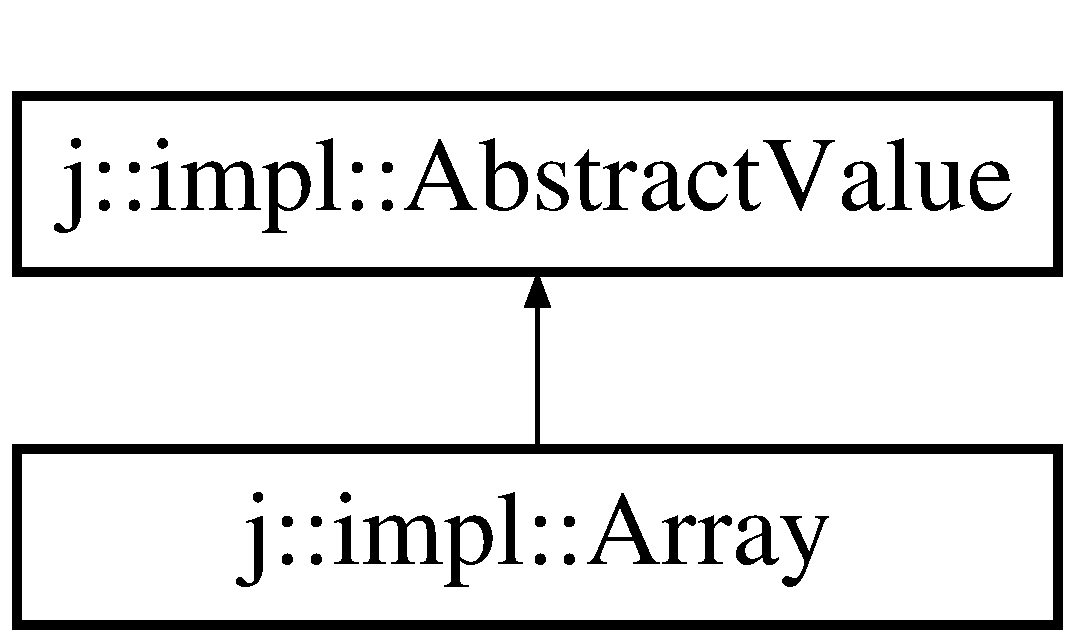
\includegraphics[height=2.000000cm]{classj_1_1impl_1_1_array}
\end{center}
\end{figure}
\subsection*{Public Member Functions}
\begin{DoxyCompactItemize}
\item 
bool \hyperlink{classj_1_1impl_1_1_array_a8878b0cfe7cac5a0d91d9f98ecc97e96}{operator==} (\hyperlink{classj_1_1impl_1_1_array}{Array} const \&other) const 
\item 
\hyperlink{classj_1_1_value}{Value} \& \hyperlink{classj_1_1impl_1_1_array_ae097ea32c79bd892dadd5d8e56190906}{operator\mbox{[}$\,$\mbox{]}} (std\-::size\-\_\-t i)
\item 
\hyperlink{classj_1_1_value}{Value} const \& \hyperlink{classj_1_1impl_1_1_array_ac77cb712be4576f67560a71afeb120df}{operator\mbox{[}$\,$\mbox{]}} (std\-::size\-\_\-t i) const 
\item 
std\-::size\-\_\-t \hyperlink{classj_1_1impl_1_1_array_af1c23f03a9674fceb428b0f8255d4c98}{size} () const 
\item 
void \hyperlink{classj_1_1impl_1_1_array_a595fc651cf671593884893cc0635d586}{add} (\hyperlink{classj_1_1_value}{Value} const \&v)
\item 
void \hyperlink{classj_1_1impl_1_1_array_ac00ba23436b735aa2e29de69a86dd6fd}{remove} (std\-::size\-\_\-t i)
\begin{DoxyCompactList}\small\item\em Remove the element at the given index. \end{DoxyCompactList}\item 
bool \hyperlink{classj_1_1impl_1_1_array_af859820f212b3bb3bb93c6bc98e756c1}{is\-Array} () const overridefinal
\item 
\hyperlink{classj_1_1impl_1_1_array}{Array} \& \hyperlink{classj_1_1impl_1_1_array_afbbbbbd781af165452dedda0a7b1ce05}{as\-Array} () overridefinal
\item 
\hyperlink{classj_1_1impl_1_1_array}{Array} const \& \hyperlink{classj_1_1impl_1_1_array_ab4ad4d8cba1ccf25cb209b03fb50573a}{as\-Array} () const overridefinal
\item 
\hyperlink{classj_1_1impl_1_1_abstract_value}{Abstract\-Value} $\ast$ \hyperlink{classj_1_1impl_1_1_array_a94e77caeb46bfcfbbf138fa75076235f}{clone} () const overridefinal
\end{DoxyCompactItemize}
\subsection*{Private Attributes}
\begin{DoxyCompactItemize}
\item 
std\-::vector$<$ std\-::unique\-\_\-ptr\\*
$<$ \hyperlink{classj_1_1_value}{Value} $>$ $>$ \hyperlink{classj_1_1impl_1_1_array_a25b3f62f6ad82d84c3c4a12723dcc070}{m\-Data}
\end{DoxyCompactItemize}


\subsection{Member Function Documentation}
\hypertarget{classj_1_1impl_1_1_array_a595fc651cf671593884893cc0635d586}{\index{j\-::impl\-::\-Array@{j\-::impl\-::\-Array}!add@{add}}
\index{add@{add}!j::impl::Array@{j\-::impl\-::\-Array}}
\subsubsection[{add}]{\setlength{\rightskip}{0pt plus 5cm}void j\-::impl\-::\-Array\-::add (
\begin{DoxyParamCaption}
\item[{{\bf Value} const \&}]{v}
\end{DoxyParamCaption}
)}}\label{classj_1_1impl_1_1_array_a595fc651cf671593884893cc0635d586}
\hypertarget{classj_1_1impl_1_1_array_afbbbbbd781af165452dedda0a7b1ce05}{\index{j\-::impl\-::\-Array@{j\-::impl\-::\-Array}!as\-Array@{as\-Array}}
\index{as\-Array@{as\-Array}!j::impl::Array@{j\-::impl\-::\-Array}}
\subsubsection[{as\-Array}]{\setlength{\rightskip}{0pt plus 5cm}{\bf Array} \& j\-::impl\-::\-Array\-::as\-Array (
\begin{DoxyParamCaption}
{}
\end{DoxyParamCaption}
)\hspace{0.3cm}{\ttfamily [final]}, {\ttfamily [override]}, {\ttfamily [virtual]}}}\label{classj_1_1impl_1_1_array_afbbbbbd781af165452dedda0a7b1ce05}


Reimplemented from \hyperlink{classj_1_1impl_1_1_abstract_value_afd41265b99a6e385f3d3cb9679d864ab}{j\-::impl\-::\-Abstract\-Value}.

\hypertarget{classj_1_1impl_1_1_array_ab4ad4d8cba1ccf25cb209b03fb50573a}{\index{j\-::impl\-::\-Array@{j\-::impl\-::\-Array}!as\-Array@{as\-Array}}
\index{as\-Array@{as\-Array}!j::impl::Array@{j\-::impl\-::\-Array}}
\subsubsection[{as\-Array}]{\setlength{\rightskip}{0pt plus 5cm}{\bf Array} const \& j\-::impl\-::\-Array\-::as\-Array (
\begin{DoxyParamCaption}
{}
\end{DoxyParamCaption}
) const\hspace{0.3cm}{\ttfamily [final]}, {\ttfamily [override]}, {\ttfamily [virtual]}}}\label{classj_1_1impl_1_1_array_ab4ad4d8cba1ccf25cb209b03fb50573a}


Reimplemented from \hyperlink{classj_1_1impl_1_1_abstract_value_ab9a29818092145c446517dda40e52b46}{j\-::impl\-::\-Abstract\-Value}.

\hypertarget{classj_1_1impl_1_1_array_a94e77caeb46bfcfbbf138fa75076235f}{\index{j\-::impl\-::\-Array@{j\-::impl\-::\-Array}!clone@{clone}}
\index{clone@{clone}!j::impl::Array@{j\-::impl\-::\-Array}}
\subsubsection[{clone}]{\setlength{\rightskip}{0pt plus 5cm}{\bf Abstract\-Value} $\ast$ j\-::impl\-::\-Array\-::clone (
\begin{DoxyParamCaption}
{}
\end{DoxyParamCaption}
) const\hspace{0.3cm}{\ttfamily [final]}, {\ttfamily [override]}, {\ttfamily [virtual]}}}\label{classj_1_1impl_1_1_array_a94e77caeb46bfcfbbf138fa75076235f}


Implements \hyperlink{classj_1_1impl_1_1_abstract_value_ac61a9aa4a4ecd3a309e8e274ac4b3dd2}{j\-::impl\-::\-Abstract\-Value}.

\hypertarget{classj_1_1impl_1_1_array_af859820f212b3bb3bb93c6bc98e756c1}{\index{j\-::impl\-::\-Array@{j\-::impl\-::\-Array}!is\-Array@{is\-Array}}
\index{is\-Array@{is\-Array}!j::impl::Array@{j\-::impl\-::\-Array}}
\subsubsection[{is\-Array}]{\setlength{\rightskip}{0pt plus 5cm}bool j\-::impl\-::\-Array\-::is\-Array (
\begin{DoxyParamCaption}
{}
\end{DoxyParamCaption}
) const\hspace{0.3cm}{\ttfamily [final]}, {\ttfamily [override]}, {\ttfamily [virtual]}}}\label{classj_1_1impl_1_1_array_af859820f212b3bb3bb93c6bc98e756c1}


Reimplemented from \hyperlink{classj_1_1impl_1_1_abstract_value_a28a367d6f2bfa668c420cc587b6daaf9}{j\-::impl\-::\-Abstract\-Value}.

\hypertarget{classj_1_1impl_1_1_array_a8878b0cfe7cac5a0d91d9f98ecc97e96}{\index{j\-::impl\-::\-Array@{j\-::impl\-::\-Array}!operator==@{operator==}}
\index{operator==@{operator==}!j::impl::Array@{j\-::impl\-::\-Array}}
\subsubsection[{operator==}]{\setlength{\rightskip}{0pt plus 5cm}bool j\-::impl\-::\-Array\-::operator== (
\begin{DoxyParamCaption}
\item[{{\bf Array} const \&}]{other}
\end{DoxyParamCaption}
) const}}\label{classj_1_1impl_1_1_array_a8878b0cfe7cac5a0d91d9f98ecc97e96}
\hypertarget{classj_1_1impl_1_1_array_ae097ea32c79bd892dadd5d8e56190906}{\index{j\-::impl\-::\-Array@{j\-::impl\-::\-Array}!operator\mbox{[}$\,$\mbox{]}@{operator[]}}
\index{operator\mbox{[}$\,$\mbox{]}@{operator[]}!j::impl::Array@{j\-::impl\-::\-Array}}
\subsubsection[{operator[]}]{\setlength{\rightskip}{0pt plus 5cm}{\bf Value} \& j\-::impl\-::\-Array\-::operator\mbox{[}$\,$\mbox{]} (
\begin{DoxyParamCaption}
\item[{std\-::size\-\_\-t}]{i}
\end{DoxyParamCaption}
)}}\label{classj_1_1impl_1_1_array_ae097ea32c79bd892dadd5d8e56190906}
\hypertarget{classj_1_1impl_1_1_array_ac77cb712be4576f67560a71afeb120df}{\index{j\-::impl\-::\-Array@{j\-::impl\-::\-Array}!operator\mbox{[}$\,$\mbox{]}@{operator[]}}
\index{operator\mbox{[}$\,$\mbox{]}@{operator[]}!j::impl::Array@{j\-::impl\-::\-Array}}
\subsubsection[{operator[]}]{\setlength{\rightskip}{0pt plus 5cm}{\bf Value} const \& j\-::impl\-::\-Array\-::operator\mbox{[}$\,$\mbox{]} (
\begin{DoxyParamCaption}
\item[{std\-::size\-\_\-t}]{i}
\end{DoxyParamCaption}
) const}}\label{classj_1_1impl_1_1_array_ac77cb712be4576f67560a71afeb120df}
\hypertarget{classj_1_1impl_1_1_array_ac00ba23436b735aa2e29de69a86dd6fd}{\index{j\-::impl\-::\-Array@{j\-::impl\-::\-Array}!remove@{remove}}
\index{remove@{remove}!j::impl::Array@{j\-::impl\-::\-Array}}
\subsubsection[{remove}]{\setlength{\rightskip}{0pt plus 5cm}void j\-::impl\-::\-Array\-::remove (
\begin{DoxyParamCaption}
\item[{std\-::size\-\_\-t}]{i}
\end{DoxyParamCaption}
)}}\label{classj_1_1impl_1_1_array_ac00ba23436b735aa2e29de69a86dd6fd}


Remove the element at the given index. 


\begin{DoxyExceptions}{Exceptions}
{\em \hyperlink{classj_1_1_no_such_element}{No\-Such\-Element}} & when the array is empty or the index is to big\\
\hline
\end{DoxyExceptions}

\begin{DoxyParams}{Parameters}
{\em i} & an index \\
\hline
\end{DoxyParams}
\hypertarget{classj_1_1impl_1_1_array_af1c23f03a9674fceb428b0f8255d4c98}{\index{j\-::impl\-::\-Array@{j\-::impl\-::\-Array}!size@{size}}
\index{size@{size}!j::impl::Array@{j\-::impl\-::\-Array}}
\subsubsection[{size}]{\setlength{\rightskip}{0pt plus 5cm}std\-::size\-\_\-t j\-::impl\-::\-Array\-::size (
\begin{DoxyParamCaption}
{}
\end{DoxyParamCaption}
) const}}\label{classj_1_1impl_1_1_array_af1c23f03a9674fceb428b0f8255d4c98}


\subsection{Member Data Documentation}
\hypertarget{classj_1_1impl_1_1_array_a25b3f62f6ad82d84c3c4a12723dcc070}{\index{j\-::impl\-::\-Array@{j\-::impl\-::\-Array}!m\-Data@{m\-Data}}
\index{m\-Data@{m\-Data}!j::impl::Array@{j\-::impl\-::\-Array}}
\subsubsection[{m\-Data}]{\setlength{\rightskip}{0pt plus 5cm}std\-::vector$<$std\-::unique\-\_\-ptr$<${\bf Value}$>$ $>$ j\-::impl\-::\-Array\-::m\-Data\hspace{0.3cm}{\ttfamily [private]}}}\label{classj_1_1impl_1_1_array_a25b3f62f6ad82d84c3c4a12723dcc070}


The documentation for this class was generated from the following files\-:\begin{DoxyCompactItemize}
\item 
/home/jbesson/myfiles/cpp/svprog/partie1/src/\-J\-S\-O\-N/\hyperlink{_j_s_o_n_impl_8hpp}{J\-S\-O\-N\-Impl.\-hpp}\item 
/home/jbesson/myfiles/cpp/svprog/partie1/src/\-J\-S\-O\-N/\hyperlink{_j_s_o_n_impl_8cpp}{J\-S\-O\-N\-Impl.\-cpp}\end{DoxyCompactItemize}

\hypertarget{structj_1_1_value_1_1_array_tag}{\section{j\-:\-:Value\-:\-:Array\-Tag Struct Reference}
\label{structj_1_1_value_1_1_array_tag}\index{j\-::\-Value\-::\-Array\-Tag@{j\-::\-Value\-::\-Array\-Tag}}
}


{\ttfamily \#include $<$J\-S\-O\-N.\-hpp$>$}



The documentation for this struct was generated from the following file\-:\begin{DoxyCompactItemize}
\item 
/home/jbesson/myfiles/cpp/svprog/partie1/src/\-J\-S\-O\-N/\hyperlink{_j_s_o_n_8hpp}{J\-S\-O\-N.\-hpp}\end{DoxyCompactItemize}

\hypertarget{classj_1_1_bad_conversion}{\section{j\-:\-:Bad\-Conversion Class Reference}
\label{classj_1_1_bad_conversion}\index{j\-::\-Bad\-Conversion@{j\-::\-Bad\-Conversion}}
}


{\ttfamily \#include $<$J\-S\-O\-N.\-hpp$>$}

Inheritance diagram for j\-:\-:Bad\-Conversion\-:\begin{figure}[H]
\begin{center}
\leavevmode
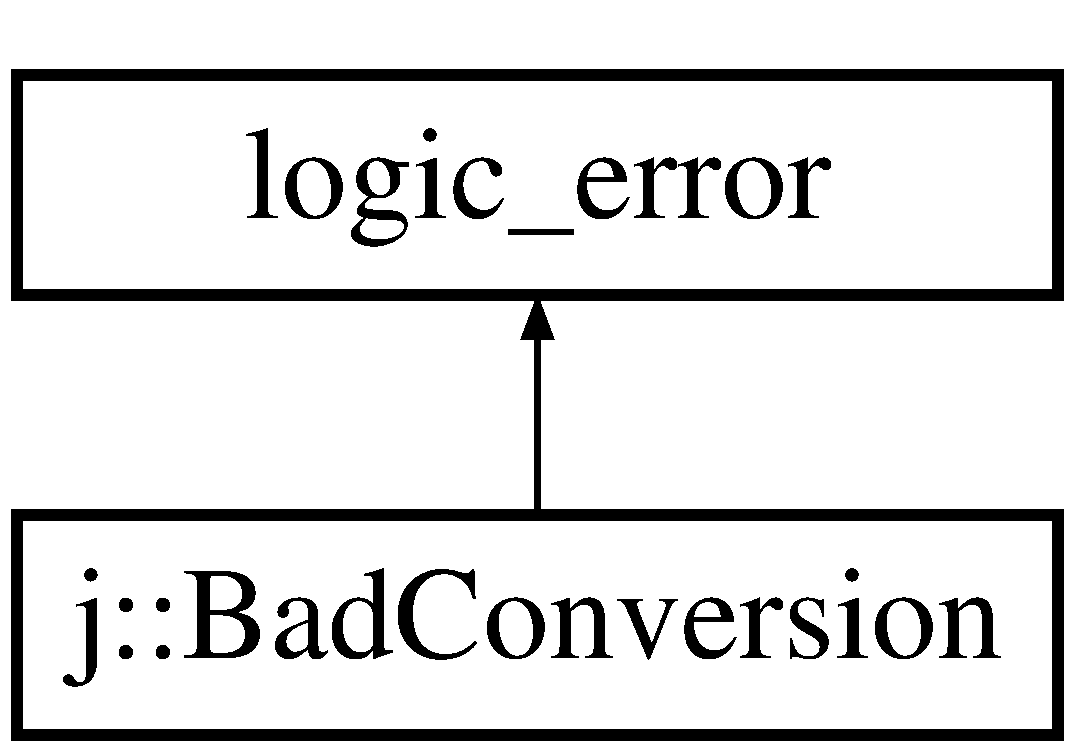
\includegraphics[height=2.000000cm]{classj_1_1_bad_conversion}
\end{center}
\end{figure}
\subsection*{Public Member Functions}
\begin{DoxyCompactItemize}
\item 
\hyperlink{classj_1_1_bad_conversion_a03fc28547084d2cbc3656f95f933fb42}{Bad\-Conversion} (std\-::string const \&from, std\-::string const \&to)
\end{DoxyCompactItemize}


\subsection{Constructor \& Destructor Documentation}
\hypertarget{classj_1_1_bad_conversion_a03fc28547084d2cbc3656f95f933fb42}{\index{j\-::\-Bad\-Conversion@{j\-::\-Bad\-Conversion}!Bad\-Conversion@{Bad\-Conversion}}
\index{Bad\-Conversion@{Bad\-Conversion}!j::BadConversion@{j\-::\-Bad\-Conversion}}
\subsubsection[{Bad\-Conversion}]{\setlength{\rightskip}{0pt plus 5cm}j\-::\-Bad\-Conversion\-::\-Bad\-Conversion (
\begin{DoxyParamCaption}
\item[{std\-::string const \&}]{from, }
\item[{std\-::string const \&}]{to}
\end{DoxyParamCaption}
)}}\label{classj_1_1_bad_conversion_a03fc28547084d2cbc3656f95f933fb42}


The documentation for this class was generated from the following files\-:\begin{DoxyCompactItemize}
\item 
/home/jbesson/myfiles/cpp/svprog/partie1/src/\-J\-S\-O\-N/\hyperlink{_j_s_o_n_8hpp}{J\-S\-O\-N.\-hpp}\item 
/home/jbesson/myfiles/cpp/svprog/partie1/src/\-J\-S\-O\-N/\hyperlink{_j_s_o_n_8cpp}{J\-S\-O\-N.\-cpp}\end{DoxyCompactItemize}

\hypertarget{classj_1_1_bad_payload}{\section{j\-:\-:Bad\-Payload Class Reference}
\label{classj_1_1_bad_payload}\index{j\-::\-Bad\-Payload@{j\-::\-Bad\-Payload}}
}


{\ttfamily \#include $<$J\-S\-O\-N\-Serialiser.\-hpp$>$}

Inheritance diagram for j\-:\-:Bad\-Payload\-:\begin{figure}[H]
\begin{center}
\leavevmode
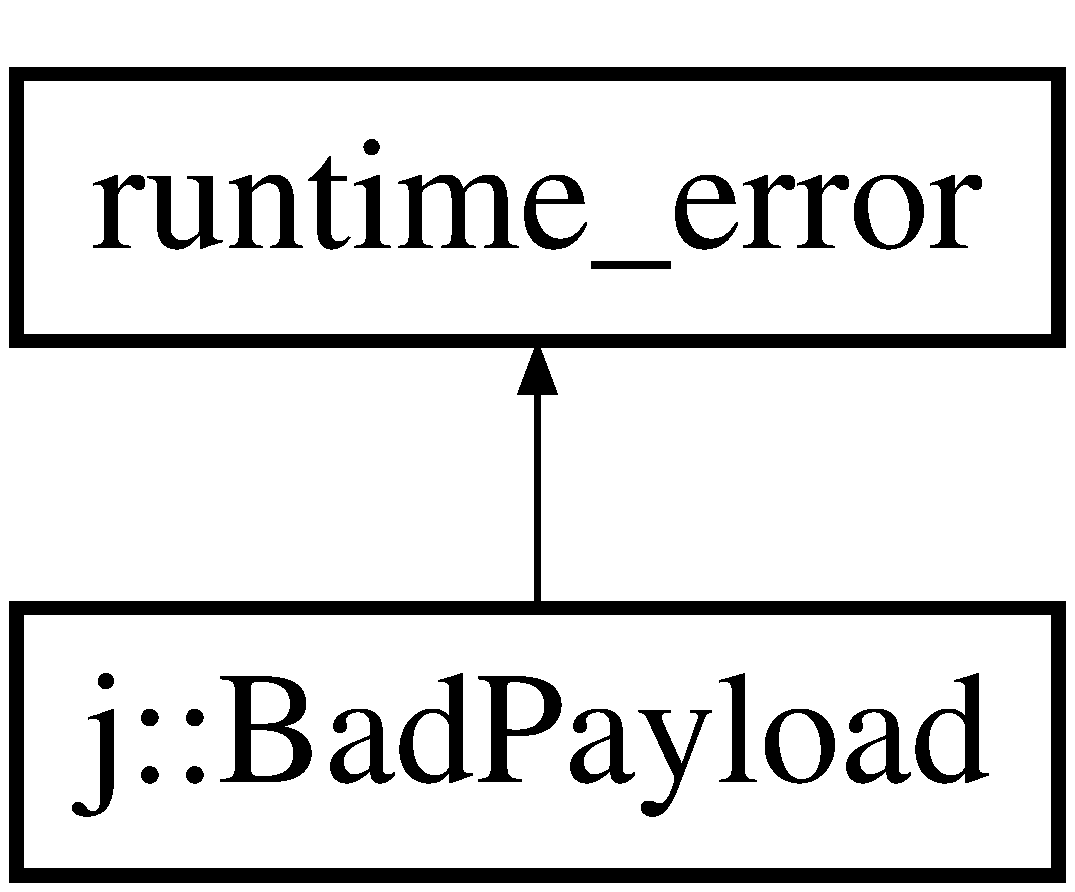
\includegraphics[height=2.000000cm]{classj_1_1_bad_payload}
\end{center}
\end{figure}
\subsection*{Public Member Functions}
\begin{DoxyCompactItemize}
\item 
\hyperlink{classj_1_1_bad_payload_a7a96b5456d6792be8060f12b4e9956a2}{Bad\-Payload} (std\-::string const \&msg)
\end{DoxyCompactItemize}


\subsection{Constructor \& Destructor Documentation}
\hypertarget{classj_1_1_bad_payload_a7a96b5456d6792be8060f12b4e9956a2}{\index{j\-::\-Bad\-Payload@{j\-::\-Bad\-Payload}!Bad\-Payload@{Bad\-Payload}}
\index{Bad\-Payload@{Bad\-Payload}!j::BadPayload@{j\-::\-Bad\-Payload}}
\subsubsection[{Bad\-Payload}]{\setlength{\rightskip}{0pt plus 5cm}j\-::\-Bad\-Payload\-::\-Bad\-Payload (
\begin{DoxyParamCaption}
\item[{std\-::string const \&}]{msg}
\end{DoxyParamCaption}
)}}\label{classj_1_1_bad_payload_a7a96b5456d6792be8060f12b4e9956a2}


The documentation for this class was generated from the following files\-:\begin{DoxyCompactItemize}
\item 
/home/jbesson/myfiles/cpp/svprog/partie1/src/\-J\-S\-O\-N/\hyperlink{_j_s_o_n_serialiser_8hpp}{J\-S\-O\-N\-Serialiser.\-hpp}\item 
/home/jbesson/myfiles/cpp/svprog/partie1/src/\-J\-S\-O\-N/\hyperlink{_j_s_o_n_serialiser_8cpp}{J\-S\-O\-N\-Serialiser.\-cpp}\end{DoxyCompactItemize}

\hypertarget{class_body}{\section{Body Class Reference}
\label{class_body}\index{Body@{Body}}
}
Inheritance diagram for Body\-:\begin{figure}[H]
\begin{center}
\leavevmode
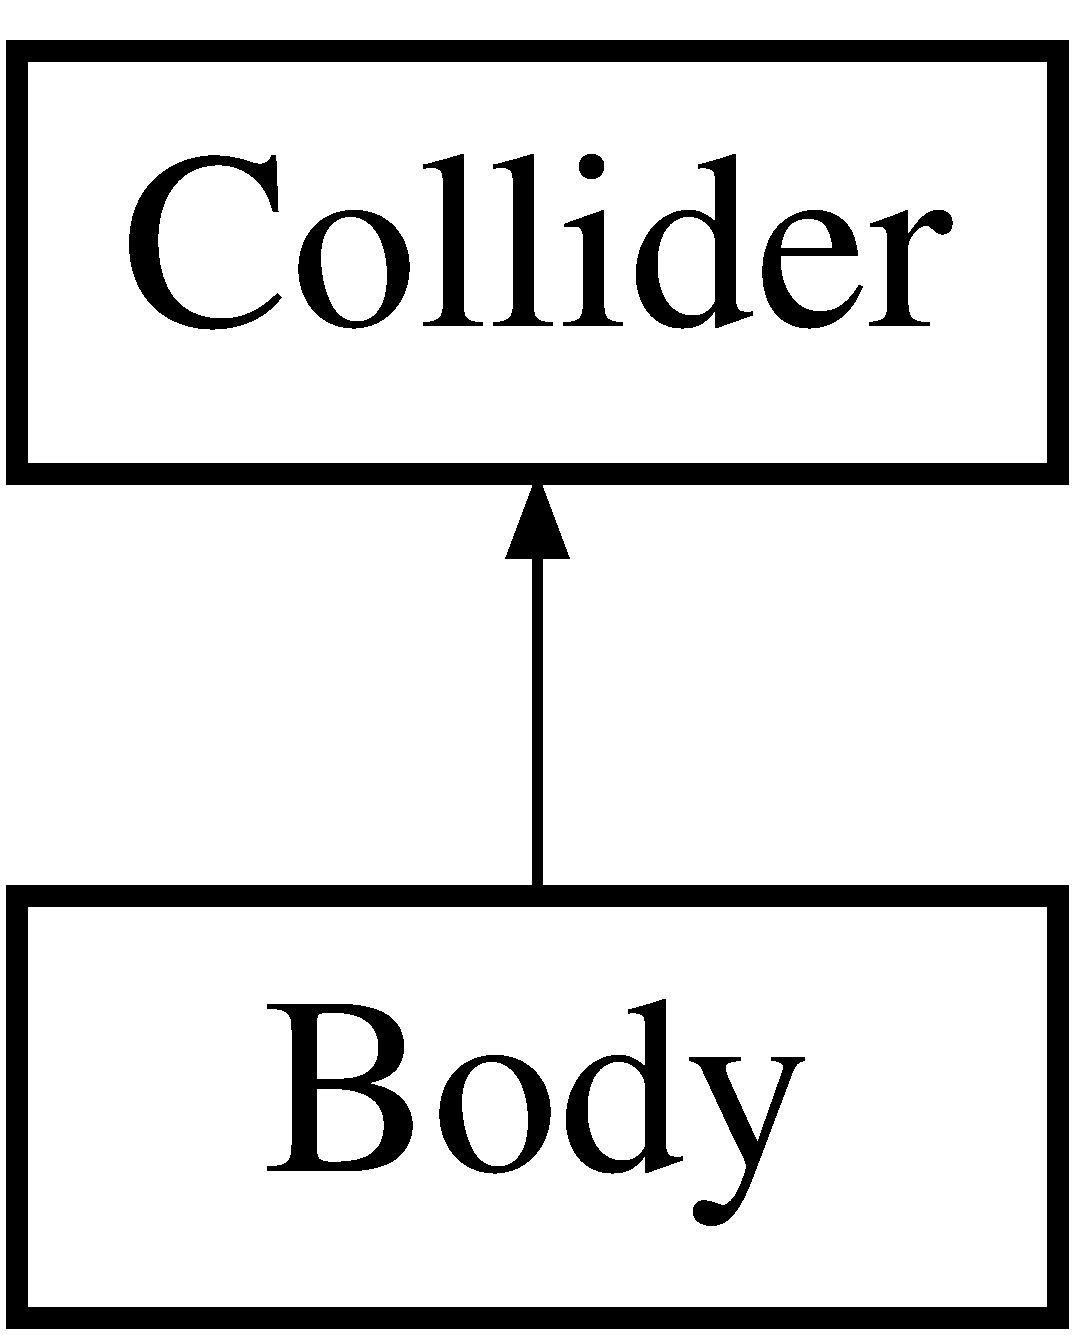
\includegraphics[height=2.000000cm]{class_body}
\end{center}
\end{figure}
\subsection*{Public Member Functions}
\begin{DoxyCompactItemize}
\item 
\hyperlink{class_body_a4a6c496c036d64ad2b5db49255bf5802}{Body} (\hyperlink{class_vec2d}{Vec2d} const \&position, double radius)
\end{DoxyCompactItemize}


\subsection{Constructor \& Destructor Documentation}
\hypertarget{class_body_a4a6c496c036d64ad2b5db49255bf5802}{\index{Body@{Body}!Body@{Body}}
\index{Body@{Body}!Body@{Body}}
\subsubsection[{Body}]{\setlength{\rightskip}{0pt plus 5cm}Body\-::\-Body (
\begin{DoxyParamCaption}
\item[{{\bf Vec2d} const \&}]{position, }
\item[{double}]{radius}
\end{DoxyParamCaption}
)\hspace{0.3cm}{\ttfamily [inline]}}}\label{class_body_a4a6c496c036d64ad2b5db49255bf5802}


The documentation for this class was generated from the following file\-:\begin{DoxyCompactItemize}
\item 
/home/jbesson/myfiles/cpp/svprog/partie1/src/\-Tests/\-Unit\-Tests/\hyperlink{_collider_test_8cpp}{Collider\-Test.\-cpp}\end{DoxyCompactItemize}

\hypertarget{classj_1_1impl_1_1_boolean}{\section{j\-:\-:impl\-:\-:Boolean Class Reference}
\label{classj_1_1impl_1_1_boolean}\index{j\-::impl\-::\-Boolean@{j\-::impl\-::\-Boolean}}
}


{\ttfamily \#include $<$J\-S\-O\-N\-Impl.\-hpp$>$}

Inheritance diagram for j\-:\-:impl\-:\-:Boolean\-:\begin{figure}[H]
\begin{center}
\leavevmode
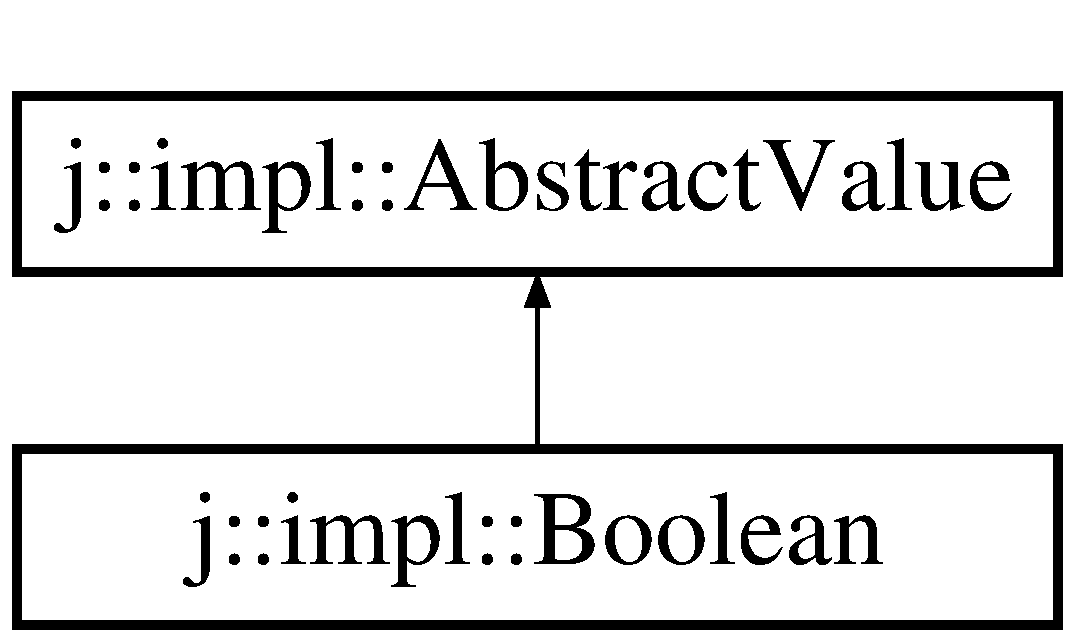
\includegraphics[height=2.000000cm]{classj_1_1impl_1_1_boolean}
\end{center}
\end{figure}
\subsection*{Public Member Functions}
\begin{DoxyCompactItemize}
\item 
\hyperlink{classj_1_1impl_1_1_boolean_ac7ab85db9285ce51045c11983ab2ae33}{Boolean} (bool b)
\item 
bool \hyperlink{classj_1_1impl_1_1_boolean_adae7a97a54365489999ccdf1495dfaaf}{to\-Bool} () const 
\item 
void \hyperlink{classj_1_1impl_1_1_boolean_adb2b2d763b3e93b7464ae87498036899}{set} (bool b)
\item 
bool \hyperlink{classj_1_1impl_1_1_boolean_ab27b415c6e0d08400ca53b5c5bcde6d2}{is\-Boolean} () const overridefinal
\item 
\hyperlink{classj_1_1impl_1_1_boolean}{Boolean} \& \hyperlink{classj_1_1impl_1_1_boolean_a1f96b1193d7fbc41bd58fed33874f2ad}{as\-Boolean} () overridefinal
\item 
\hyperlink{classj_1_1impl_1_1_boolean}{Boolean} const \& \hyperlink{classj_1_1impl_1_1_boolean_a174f6cfb37900f17708bf4fb34d94aa6}{as\-Boolean} () const overridefinal
\item 
\hyperlink{classj_1_1impl_1_1_abstract_value}{Abstract\-Value} $\ast$ \hyperlink{classj_1_1impl_1_1_boolean_a299b417212ed86a52b08e2bdbd6921f0}{clone} () const overridefinal
\end{DoxyCompactItemize}
\subsection*{Private Attributes}
\begin{DoxyCompactItemize}
\item 
bool \hyperlink{classj_1_1impl_1_1_boolean_ac527e412a7be3cc4c170eccb06256ea3}{m\-Bool}
\end{DoxyCompactItemize}


\subsection{Constructor \& Destructor Documentation}
\hypertarget{classj_1_1impl_1_1_boolean_ac7ab85db9285ce51045c11983ab2ae33}{\index{j\-::impl\-::\-Boolean@{j\-::impl\-::\-Boolean}!Boolean@{Boolean}}
\index{Boolean@{Boolean}!j::impl::Boolean@{j\-::impl\-::\-Boolean}}
\subsubsection[{Boolean}]{\setlength{\rightskip}{0pt plus 5cm}j\-::impl\-::\-Boolean\-::\-Boolean (
\begin{DoxyParamCaption}
\item[{bool}]{b}
\end{DoxyParamCaption}
)}}\label{classj_1_1impl_1_1_boolean_ac7ab85db9285ce51045c11983ab2ae33}


\subsection{Member Function Documentation}
\hypertarget{classj_1_1impl_1_1_boolean_a1f96b1193d7fbc41bd58fed33874f2ad}{\index{j\-::impl\-::\-Boolean@{j\-::impl\-::\-Boolean}!as\-Boolean@{as\-Boolean}}
\index{as\-Boolean@{as\-Boolean}!j::impl::Boolean@{j\-::impl\-::\-Boolean}}
\subsubsection[{as\-Boolean}]{\setlength{\rightskip}{0pt plus 5cm}{\bf Boolean} \& j\-::impl\-::\-Boolean\-::as\-Boolean (
\begin{DoxyParamCaption}
{}
\end{DoxyParamCaption}
)\hspace{0.3cm}{\ttfamily [final]}, {\ttfamily [override]}, {\ttfamily [virtual]}}}\label{classj_1_1impl_1_1_boolean_a1f96b1193d7fbc41bd58fed33874f2ad}


Reimplemented from \hyperlink{classj_1_1impl_1_1_abstract_value_ae658e600ec0589f3a632a803fa390ad4}{j\-::impl\-::\-Abstract\-Value}.

\hypertarget{classj_1_1impl_1_1_boolean_a174f6cfb37900f17708bf4fb34d94aa6}{\index{j\-::impl\-::\-Boolean@{j\-::impl\-::\-Boolean}!as\-Boolean@{as\-Boolean}}
\index{as\-Boolean@{as\-Boolean}!j::impl::Boolean@{j\-::impl\-::\-Boolean}}
\subsubsection[{as\-Boolean}]{\setlength{\rightskip}{0pt plus 5cm}{\bf Boolean} const \& j\-::impl\-::\-Boolean\-::as\-Boolean (
\begin{DoxyParamCaption}
{}
\end{DoxyParamCaption}
) const\hspace{0.3cm}{\ttfamily [final]}, {\ttfamily [override]}, {\ttfamily [virtual]}}}\label{classj_1_1impl_1_1_boolean_a174f6cfb37900f17708bf4fb34d94aa6}


Reimplemented from \hyperlink{classj_1_1impl_1_1_abstract_value_a19f38830cc9b55aa22c5eb41868b56c2}{j\-::impl\-::\-Abstract\-Value}.

\hypertarget{classj_1_1impl_1_1_boolean_a299b417212ed86a52b08e2bdbd6921f0}{\index{j\-::impl\-::\-Boolean@{j\-::impl\-::\-Boolean}!clone@{clone}}
\index{clone@{clone}!j::impl::Boolean@{j\-::impl\-::\-Boolean}}
\subsubsection[{clone}]{\setlength{\rightskip}{0pt plus 5cm}{\bf Abstract\-Value} $\ast$ j\-::impl\-::\-Boolean\-::clone (
\begin{DoxyParamCaption}
{}
\end{DoxyParamCaption}
) const\hspace{0.3cm}{\ttfamily [final]}, {\ttfamily [override]}, {\ttfamily [virtual]}}}\label{classj_1_1impl_1_1_boolean_a299b417212ed86a52b08e2bdbd6921f0}


Implements \hyperlink{classj_1_1impl_1_1_abstract_value_ac61a9aa4a4ecd3a309e8e274ac4b3dd2}{j\-::impl\-::\-Abstract\-Value}.

\hypertarget{classj_1_1impl_1_1_boolean_ab27b415c6e0d08400ca53b5c5bcde6d2}{\index{j\-::impl\-::\-Boolean@{j\-::impl\-::\-Boolean}!is\-Boolean@{is\-Boolean}}
\index{is\-Boolean@{is\-Boolean}!j::impl::Boolean@{j\-::impl\-::\-Boolean}}
\subsubsection[{is\-Boolean}]{\setlength{\rightskip}{0pt plus 5cm}bool j\-::impl\-::\-Boolean\-::is\-Boolean (
\begin{DoxyParamCaption}
{}
\end{DoxyParamCaption}
) const\hspace{0.3cm}{\ttfamily [final]}, {\ttfamily [override]}, {\ttfamily [virtual]}}}\label{classj_1_1impl_1_1_boolean_ab27b415c6e0d08400ca53b5c5bcde6d2}


Reimplemented from \hyperlink{classj_1_1impl_1_1_abstract_value_a057ddc8b2d01c7a93b998cf1fab01cdd}{j\-::impl\-::\-Abstract\-Value}.

\hypertarget{classj_1_1impl_1_1_boolean_adb2b2d763b3e93b7464ae87498036899}{\index{j\-::impl\-::\-Boolean@{j\-::impl\-::\-Boolean}!set@{set}}
\index{set@{set}!j::impl::Boolean@{j\-::impl\-::\-Boolean}}
\subsubsection[{set}]{\setlength{\rightskip}{0pt plus 5cm}void j\-::impl\-::\-Boolean\-::set (
\begin{DoxyParamCaption}
\item[{bool}]{b}
\end{DoxyParamCaption}
)}}\label{classj_1_1impl_1_1_boolean_adb2b2d763b3e93b7464ae87498036899}
\hypertarget{classj_1_1impl_1_1_boolean_adae7a97a54365489999ccdf1495dfaaf}{\index{j\-::impl\-::\-Boolean@{j\-::impl\-::\-Boolean}!to\-Bool@{to\-Bool}}
\index{to\-Bool@{to\-Bool}!j::impl::Boolean@{j\-::impl\-::\-Boolean}}
\subsubsection[{to\-Bool}]{\setlength{\rightskip}{0pt plus 5cm}bool j\-::impl\-::\-Boolean\-::to\-Bool (
\begin{DoxyParamCaption}
{}
\end{DoxyParamCaption}
) const}}\label{classj_1_1impl_1_1_boolean_adae7a97a54365489999ccdf1495dfaaf}


\subsection{Member Data Documentation}
\hypertarget{classj_1_1impl_1_1_boolean_ac527e412a7be3cc4c170eccb06256ea3}{\index{j\-::impl\-::\-Boolean@{j\-::impl\-::\-Boolean}!m\-Bool@{m\-Bool}}
\index{m\-Bool@{m\-Bool}!j::impl::Boolean@{j\-::impl\-::\-Boolean}}
\subsubsection[{m\-Bool}]{\setlength{\rightskip}{0pt plus 5cm}bool j\-::impl\-::\-Boolean\-::m\-Bool\hspace{0.3cm}{\ttfamily [private]}}}\label{classj_1_1impl_1_1_boolean_ac527e412a7be3cc4c170eccb06256ea3}


The documentation for this class was generated from the following files\-:\begin{DoxyCompactItemize}
\item 
/home/jbesson/myfiles/cpp/svprog/partie1/src/\-J\-S\-O\-N/\hyperlink{_j_s_o_n_impl_8hpp}{J\-S\-O\-N\-Impl.\-hpp}\item 
/home/jbesson/myfiles/cpp/svprog/partie1/src/\-J\-S\-O\-N/\hyperlink{_j_s_o_n_impl_8cpp}{J\-S\-O\-N\-Impl.\-cpp}\end{DoxyCompactItemize}

\hypertarget{class_collider}{\section{Collider Class Reference}
\label{class_collider}\index{Collider@{Collider}}
}


{\ttfamily \#include $<$Collider.\-hpp$>$}

Inheritance diagram for Collider\-:\begin{figure}[H]
\begin{center}
\leavevmode
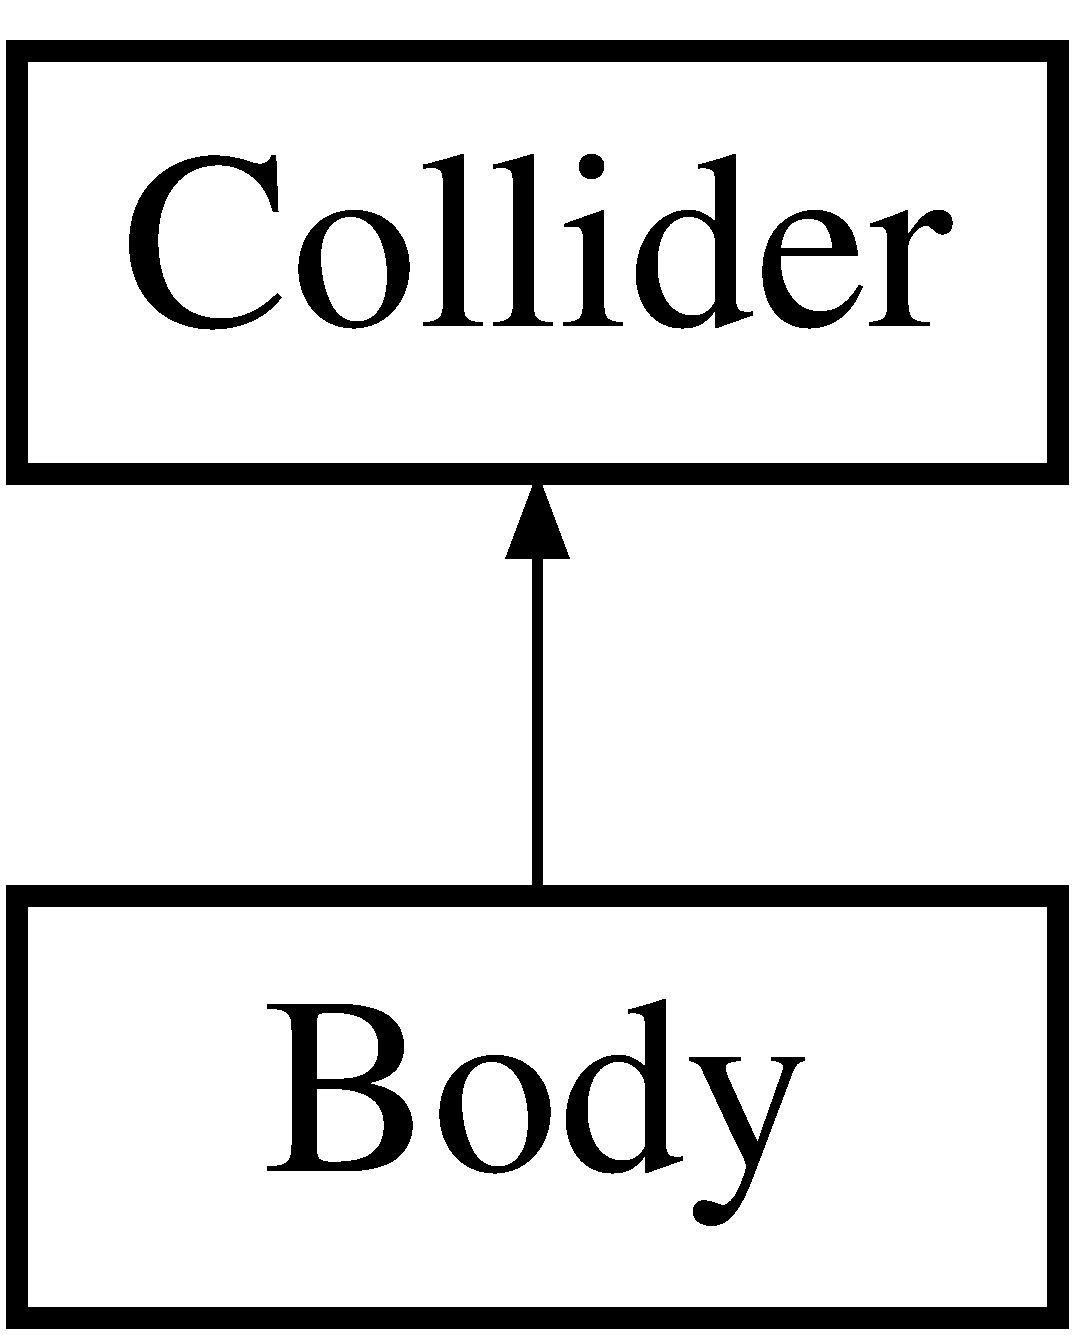
\includegraphics[height=2.000000cm]{class_collider}
\end{center}
\end{figure}
\subsection*{Public Member Functions}
\begin{DoxyCompactItemize}
\item 
\hyperlink{class_collider_ad836873a098459ff45f7441e2a392965}{Collider} (const \hyperlink{class_vec2d}{Vec2d} \&position, double radius)
\item 
\hyperlink{class_collider_a558cb702fc3472adb0a0582c5fd086ee}{Collider} (const \hyperlink{class_collider}{Collider} \&collider)
\item 
bool \hyperlink{class_collider_abcff9ab2aed0f2c203a40992021cac5c}{operator$>$} (const \hyperlink{class_collider}{Collider} \&other) const 
\item 
bool \hyperlink{class_collider_afbb568e5d59403e71ab923a3434a1ace}{operator$\vert$} (const \hyperlink{class_collider}{Collider} \&other) const 
\item 
bool \hyperlink{class_collider_a6aa51611a7dba5cf61f6a244fdc595d3}{operator$>$} (const \hyperlink{class_vec2d}{Vec2d} \&p) const 
\item 
\hyperlink{class_collider}{Collider} \& \hyperlink{class_collider_ab00523233915a797a29cd1c1afaf902e}{operator=} (\hyperlink{class_collider}{Collider} collider)
\item 
\hyperlink{class_collider}{Collider} \& \hyperlink{class_collider_ab87384b560241dc5c311fe8445883146}{operator+=} (const \hyperlink{class_vec2d}{Vec2d} \&dx)
\item 
\hyperlink{class_vec2d}{Vec2d} \hyperlink{class_collider_ad7d4e7416f8656185187ce091636c415}{clamping} ()
\item 
bool \hyperlink{class_collider_a7c95964c0df6bdc17affb9c895529a78}{is\-Collider\-Inside} (const \hyperlink{class_collider}{Collider} \&other) const 
\item 
bool \hyperlink{class_collider_a9956c286daeba882bbf6bc8dd4b1b646}{is\-Colliding} (const \hyperlink{class_collider}{Collider} \&other) const 
\item 
bool \hyperlink{class_collider_aa2513b48f566bc1ef1870018a37e7e59}{is\-Point\-Inside} (const \hyperlink{class_vec2d}{Vec2d} \&p) const 
\item 
\hyperlink{class_vec2d}{Vec2d} \hyperlink{class_collider_a0c5fb5c53e890eed9de59cdc91bfd1a6}{direction\-To} (const \hyperlink{class_vec2d}{Vec2d} \&other) const 
\item 
\hyperlink{class_vec2d}{Vec2d} \hyperlink{class_collider_a23fb77a557f53fe080c492cb19fc2fe7}{direction\-To} (const \hyperlink{class_collider}{Collider} \&other) const 
\item 
double \hyperlink{class_collider_ad8d7202a4cab50704bdb17012dea8ffa}{distance\-To} (const \hyperlink{class_vec2d}{Vec2d} \&other) const 
\item 
double \hyperlink{class_collider_a69c933446d5804c6668e874239aae77f}{distance\-To} (const \hyperlink{class_collider}{Collider} \&other) const 
\item 
\hyperlink{class_collider}{Collider} \& \hyperlink{class_collider_a6f7e2accc954f5852f83ff487f156aff}{move} (const \hyperlink{class_vec2d}{Vec2d} \&dx)
\item 
\hyperlink{class_vec2d}{Vec2d} \hyperlink{class_collider_a1893928580356ec0c1ca7cbbbd2e4ab3}{get\-Position} () const 
\item 
double \hyperlink{class_collider_a89b739bb04aea802f0cd2f36d3367711}{get\-Radius} () const 
\end{DoxyCompactItemize}
\subsection*{Private Attributes}
\begin{DoxyCompactItemize}
\item 
double \hyperlink{class_collider_a762d208b956ffa20644243c8eb8ebefa}{radius\-\_\-}
\item 
\hyperlink{class_vec2d}{Vec2d} \hyperlink{class_collider_a6e88f831b1ca9fb7a99637be1ac1570f}{position\-\_\-}
\end{DoxyCompactItemize}


\subsection{Detailed Description}
Allows checking for object collisions. Methods allow checking for collisions in between class implementations. 

\subsection{Constructor \& Destructor Documentation}
\hypertarget{class_collider_ad836873a098459ff45f7441e2a392965}{\index{Collider@{Collider}!Collider@{Collider}}
\index{Collider@{Collider}!Collider@{Collider}}
\subsubsection[{Collider}]{\setlength{\rightskip}{0pt plus 5cm}Collider\-::\-Collider (
\begin{DoxyParamCaption}
\item[{const {\bf Vec2d} \&}]{position, }
\item[{double}]{radius}
\end{DoxyParamCaption}
)}}\label{class_collider_ad836873a098459ff45f7441e2a392965}
Class constructor. Construct a \hyperlink{class_collider}{Collider} from a postions and a radius. 
\begin{DoxyParams}{Parameters}
{\em position} & vector of the \hyperlink{class_collider}{Collider} \\
\hline
{\em radius} & radius of the \hyperlink{class_collider}{Collider} \\
\hline
\end{DoxyParams}
\hypertarget{class_collider_a558cb702fc3472adb0a0582c5fd086ee}{\index{Collider@{Collider}!Collider@{Collider}}
\index{Collider@{Collider}!Collider@{Collider}}
\subsubsection[{Collider}]{\setlength{\rightskip}{0pt plus 5cm}Collider\-::\-Collider (
\begin{DoxyParamCaption}
\item[{const {\bf Collider} \&}]{collider}
\end{DoxyParamCaption}
)}}\label{class_collider_a558cb702fc3472adb0a0582c5fd086ee}
Copy constructor. Copy all the atttributes from another \hyperlink{class_collider}{Collider}. 

\subsection{Member Function Documentation}
\hypertarget{class_collider_ad7d4e7416f8656185187ce091636c415}{\index{Collider@{Collider}!clamping@{clamping}}
\index{clamping@{clamping}!Collider@{Collider}}
\subsubsection[{clamping}]{\setlength{\rightskip}{0pt plus 5cm}{\bf Vec2d} Collider\-::clamping (
\begin{DoxyParamCaption}
{}
\end{DoxyParamCaption}
)}}\label{class_collider_ad7d4e7416f8656185187ce091636c415}
Clamping method checks that position is within toric grid. This method will check that the position is not on a different face of the world, and will correct the position if it is. \hypertarget{class_collider_a0c5fb5c53e890eed9de59cdc91bfd1a6}{\index{Collider@{Collider}!direction\-To@{direction\-To}}
\index{direction\-To@{direction\-To}!Collider@{Collider}}
\subsubsection[{direction\-To}]{\setlength{\rightskip}{0pt plus 5cm}{\bf Vec2d} Collider\-::direction\-To (
\begin{DoxyParamCaption}
\item[{const {\bf Vec2d} \&}]{other}
\end{DoxyParamCaption}
) const}}\label{class_collider_a0c5fb5c53e890eed9de59cdc91bfd1a6}
Calculate the shortest toric path to a position on the grid. \begin{DoxyReturn}{Returns}
direction vector to other. 
\end{DoxyReturn}

\begin{DoxyParams}{Parameters}
{\em other} & A position on the grid. \\
\hline
\end{DoxyParams}
\hypertarget{class_collider_a23fb77a557f53fe080c492cb19fc2fe7}{\index{Collider@{Collider}!direction\-To@{direction\-To}}
\index{direction\-To@{direction\-To}!Collider@{Collider}}
\subsubsection[{direction\-To}]{\setlength{\rightskip}{0pt plus 5cm}{\bf Vec2d} Collider\-::direction\-To (
\begin{DoxyParamCaption}
\item[{const {\bf Collider} \&}]{other}
\end{DoxyParamCaption}
) const}}\label{class_collider_a23fb77a557f53fe080c492cb19fc2fe7}
Calculate the shortest toric path to another \hyperlink{class_collider}{Collider} on the grid. \begin{DoxyReturn}{Returns}
direction vector to other. 
\end{DoxyReturn}

\begin{DoxyParams}{Parameters}
{\em other} & Another \hyperlink{class_collider}{Collider}. \\
\hline
\end{DoxyParams}
\hypertarget{class_collider_ad8d7202a4cab50704bdb17012dea8ffa}{\index{Collider@{Collider}!distance\-To@{distance\-To}}
\index{distance\-To@{distance\-To}!Collider@{Collider}}
\subsubsection[{distance\-To}]{\setlength{\rightskip}{0pt plus 5cm}double Collider\-::distance\-To (
\begin{DoxyParamCaption}
\item[{const {\bf Vec2d} \&}]{other}
\end{DoxyParamCaption}
) const}}\label{class_collider_ad8d7202a4cab50704bdb17012dea8ffa}
\begin{DoxyReturn}{Returns}
distance to other. 
\end{DoxyReturn}

\begin{DoxyParams}{Parameters}
{\em other} & A position on the grid. \\
\hline
\end{DoxyParams}
\hypertarget{class_collider_a69c933446d5804c6668e874239aae77f}{\index{Collider@{Collider}!distance\-To@{distance\-To}}
\index{distance\-To@{distance\-To}!Collider@{Collider}}
\subsubsection[{distance\-To}]{\setlength{\rightskip}{0pt plus 5cm}double Collider\-::distance\-To (
\begin{DoxyParamCaption}
\item[{const {\bf Collider} \&}]{other}
\end{DoxyParamCaption}
) const}}\label{class_collider_a69c933446d5804c6668e874239aae77f}
\begin{DoxyReturn}{Returns}
distance to other. 
\end{DoxyReturn}

\begin{DoxyParams}{Parameters}
{\em collider} & another \hyperlink{class_collider}{Collider} \\
\hline
\end{DoxyParams}
\hypertarget{class_collider_a1893928580356ec0c1ca7cbbbd2e4ab3}{\index{Collider@{Collider}!get\-Position@{get\-Position}}
\index{get\-Position@{get\-Position}!Collider@{Collider}}
\subsubsection[{get\-Position}]{\setlength{\rightskip}{0pt plus 5cm}{\bf Vec2d} Collider\-::get\-Position (
\begin{DoxyParamCaption}
{}
\end{DoxyParamCaption}
) const}}\label{class_collider_a1893928580356ec0c1ca7cbbbd2e4ab3}
Get the position. \begin{DoxyReturn}{Returns}
position of this \hyperlink{class_collider}{Collider}. 
\end{DoxyReturn}
\hypertarget{class_collider_a89b739bb04aea802f0cd2f36d3367711}{\index{Collider@{Collider}!get\-Radius@{get\-Radius}}
\index{get\-Radius@{get\-Radius}!Collider@{Collider}}
\subsubsection[{get\-Radius}]{\setlength{\rightskip}{0pt plus 5cm}double Collider\-::get\-Radius (
\begin{DoxyParamCaption}
{}
\end{DoxyParamCaption}
) const}}\label{class_collider_a89b739bb04aea802f0cd2f36d3367711}
Get the radius. \begin{DoxyReturn}{Returns}
radius of this \hyperlink{class_collider}{Collider}. 
\end{DoxyReturn}
\hypertarget{class_collider_a7c95964c0df6bdc17affb9c895529a78}{\index{Collider@{Collider}!is\-Collider\-Inside@{is\-Collider\-Inside}}
\index{is\-Collider\-Inside@{is\-Collider\-Inside}!Collider@{Collider}}
\subsubsection[{is\-Collider\-Inside}]{\setlength{\rightskip}{0pt plus 5cm}bool Collider\-::is\-Collider\-Inside (
\begin{DoxyParamCaption}
\item[{const {\bf Collider} \&}]{other}
\end{DoxyParamCaption}
) const}}\label{class_collider_a7c95964c0df6bdc17affb9c895529a78}
Check if other is in this \hyperlink{class_collider}{Collider} \begin{DoxyReturn}{Returns}
true if this is within radius of other. 
\end{DoxyReturn}
\hypertarget{class_collider_a9956c286daeba882bbf6bc8dd4b1b646}{\index{Collider@{Collider}!is\-Colliding@{is\-Colliding}}
\index{is\-Colliding@{is\-Colliding}!Collider@{Collider}}
\subsubsection[{is\-Colliding}]{\setlength{\rightskip}{0pt plus 5cm}bool Collider\-::is\-Colliding (
\begin{DoxyParamCaption}
\item[{const {\bf Collider} \&}]{other}
\end{DoxyParamCaption}
) const}}\label{class_collider_a9956c286daeba882bbf6bc8dd4b1b646}
\begin{DoxyReturn}{Returns}
true if either of this or other are within the others radius. 
\end{DoxyReturn}
\hypertarget{class_collider_aa2513b48f566bc1ef1870018a37e7e59}{\index{Collider@{Collider}!is\-Point\-Inside@{is\-Point\-Inside}}
\index{is\-Point\-Inside@{is\-Point\-Inside}!Collider@{Collider}}
\subsubsection[{is\-Point\-Inside}]{\setlength{\rightskip}{0pt plus 5cm}bool Collider\-::is\-Point\-Inside (
\begin{DoxyParamCaption}
\item[{const {\bf Vec2d} \&}]{p}
\end{DoxyParamCaption}
) const}}\label{class_collider_aa2513b48f566bc1ef1870018a37e7e59}
\begin{DoxyReturn}{Returns}
true is distance in between p and this $<$ radius\-\_\-. 
\end{DoxyReturn}
\hypertarget{class_collider_a6f7e2accc954f5852f83ff487f156aff}{\index{Collider@{Collider}!move@{move}}
\index{move@{move}!Collider@{Collider}}
\subsubsection[{move}]{\setlength{\rightskip}{0pt plus 5cm}{\bf Collider} \& Collider\-::move (
\begin{DoxyParamCaption}
\item[{const {\bf Vec2d} \&}]{dx}
\end{DoxyParamCaption}
)}}\label{class_collider_a6f7e2accc954f5852f83ff487f156aff}
move this \hyperlink{class_collider}{Collider} by the vector dx. 
\begin{DoxyParams}{Parameters}
{\em dx} & Vector to move \hyperlink{class_collider}{Collider} by. \\
\hline
\end{DoxyParams}
\hypertarget{class_collider_ab87384b560241dc5c311fe8445883146}{\index{Collider@{Collider}!operator+=@{operator+=}}
\index{operator+=@{operator+=}!Collider@{Collider}}
\subsubsection[{operator+=}]{\setlength{\rightskip}{0pt plus 5cm}{\bf Collider} \& Collider\-::operator+= (
\begin{DoxyParamCaption}
\item[{const {\bf Vec2d} \&}]{dx}
\end{DoxyParamCaption}
)}}\label{class_collider_ab87384b560241dc5c311fe8445883146}
Move this horizontaly by dx. 
\begin{DoxyParams}{Parameters}
{\em Vector} & to move this \hyperlink{class_collider}{Collider} by. \\
\hline
\end{DoxyParams}
\hypertarget{class_collider_ab00523233915a797a29cd1c1afaf902e}{\index{Collider@{Collider}!operator=@{operator=}}
\index{operator=@{operator=}!Collider@{Collider}}
\subsubsection[{operator=}]{\setlength{\rightskip}{0pt plus 5cm}{\bf Collider} \& Collider\-::operator= (
\begin{DoxyParamCaption}
\item[{{\bf Collider}}]{collider}
\end{DoxyParamCaption}
)}}\label{class_collider_ab00523233915a797a29cd1c1afaf902e}
Copy opperator, call to copy constructor. 
\begin{DoxyParams}{Parameters}
{\em collider} & \hyperlink{class_collider}{Collider} to copy from. \\
\hline
\end{DoxyParams}
\hypertarget{class_collider_abcff9ab2aed0f2c203a40992021cac5c}{\index{Collider@{Collider}!operator$>$@{operator$>$}}
\index{operator$>$@{operator$>$}!Collider@{Collider}}
\subsubsection[{operator$>$}]{\setlength{\rightskip}{0pt plus 5cm}bool Collider\-::operator$>$ (
\begin{DoxyParamCaption}
\item[{const {\bf Collider} \&}]{other}
\end{DoxyParamCaption}
) const}}\label{class_collider_abcff9ab2aed0f2c203a40992021cac5c}
Check if other is in this. 
\begin{DoxyParams}{Parameters}
{\em other} & another collider. \\
\hline
\end{DoxyParams}
\begin{DoxyReturn}{Returns}
true if other is in this. 
\end{DoxyReturn}
\hypertarget{class_collider_a6aa51611a7dba5cf61f6a244fdc595d3}{\index{Collider@{Collider}!operator$>$@{operator$>$}}
\index{operator$>$@{operator$>$}!Collider@{Collider}}
\subsubsection[{operator$>$}]{\setlength{\rightskip}{0pt plus 5cm}bool Collider\-::operator$>$ (
\begin{DoxyParamCaption}
\item[{const {\bf Vec2d} \&}]{p}
\end{DoxyParamCaption}
) const}}\label{class_collider_a6aa51611a7dba5cf61f6a244fdc595d3}
Check if a point p is in the collider. 
\begin{DoxyParams}{Parameters}
{\em p} & a vector point \\
\hline
\end{DoxyParams}
\begin{DoxyReturn}{Returns}
true if point p is within radius\-\_\- of this. 
\end{DoxyReturn}
\hypertarget{class_collider_afbb568e5d59403e71ab923a3434a1ace}{\index{Collider@{Collider}!operator$\vert$@{operator$\vert$}}
\index{operator$\vert$@{operator$\vert$}!Collider@{Collider}}
\subsubsection[{operator$\vert$}]{\setlength{\rightskip}{0pt plus 5cm}bool Collider\-::operator$\vert$ (
\begin{DoxyParamCaption}
\item[{const {\bf Collider} \&}]{other}
\end{DoxyParamCaption}
) const}}\label{class_collider_afbb568e5d59403e71ab923a3434a1ace}
Check if this \hyperlink{class_collider}{Collider} is colliding with another. 
\begin{DoxyParams}{Parameters}
{\em other} & another collider. \\
\hline
\end{DoxyParams}
\begin{DoxyReturn}{Returns}
true if this is colliding with other. 
\end{DoxyReturn}


\subsection{Member Data Documentation}
\hypertarget{class_collider_a6e88f831b1ca9fb7a99637be1ac1570f}{\index{Collider@{Collider}!position\-\_\-@{position\-\_\-}}
\index{position\-\_\-@{position\-\_\-}!Collider@{Collider}}
\subsubsection[{position\-\_\-}]{\setlength{\rightskip}{0pt plus 5cm}{\bf Vec2d} Collider\-::position\-\_\-\hspace{0.3cm}{\ttfamily [private]}}}\label{class_collider_a6e88f831b1ca9fb7a99637be1ac1570f}
radius of this \hyperlink{class_collider}{Collider}. \hypertarget{class_collider_a762d208b956ffa20644243c8eb8ebefa}{\index{Collider@{Collider}!radius\-\_\-@{radius\-\_\-}}
\index{radius\-\_\-@{radius\-\_\-}!Collider@{Collider}}
\subsubsection[{radius\-\_\-}]{\setlength{\rightskip}{0pt plus 5cm}double Collider\-::radius\-\_\-\hspace{0.3cm}{\ttfamily [private]}}}\label{class_collider_a762d208b956ffa20644243c8eb8ebefa}


The documentation for this class was generated from the following files\-:\begin{DoxyCompactItemize}
\item 
/home/jbesson/myfiles/cpp/svprog/partie1/src/\-Env/\hyperlink{_collider_8hpp}{Collider.\-hpp}\item 
/home/jbesson/myfiles/cpp/svprog/partie1/src/\-Env/\hyperlink{_collider_8cpp}{Collider.\-cpp}\end{DoxyCompactItemize}

\hypertarget{class_drawable}{\section{Drawable Class Reference}
\label{class_drawable}\index{Drawable@{Drawable}}
}


Represents an entity that can be represented graphically.  




{\ttfamily \#include $<$Drawable.\-hpp$>$}

\subsection*{Public Member Functions}
\begin{DoxyCompactItemize}
\item 
virtual \hyperlink{class_drawable_a489905d7db51e37ceee8fc7eaff6a762}{$\sim$\-Drawable} ()=default
\item 
virtual void \hyperlink{class_drawable_ac25da182d04a0a681e214ca7b12bd997}{draw\-On} (sf\-::\-Render\-Target \&target) const =0
\end{DoxyCompactItemize}


\subsection{Detailed Description}
Represents an entity that can be represented graphically. 

\subsection{Constructor \& Destructor Documentation}
\hypertarget{class_drawable_a489905d7db51e37ceee8fc7eaff6a762}{\index{Drawable@{Drawable}!$\sim$\-Drawable@{$\sim$\-Drawable}}
\index{$\sim$\-Drawable@{$\sim$\-Drawable}!Drawable@{Drawable}}
\subsubsection[{$\sim$\-Drawable}]{\setlength{\rightskip}{0pt plus 5cm}virtual Drawable\-::$\sim$\-Drawable (
\begin{DoxyParamCaption}
{}
\end{DoxyParamCaption}
)\hspace{0.3cm}{\ttfamily [virtual]}, {\ttfamily [default]}}}\label{class_drawable_a489905d7db51e37ceee8fc7eaff6a762}


\subsection{Member Function Documentation}
\hypertarget{class_drawable_ac25da182d04a0a681e214ca7b12bd997}{\index{Drawable@{Drawable}!draw\-On@{draw\-On}}
\index{draw\-On@{draw\-On}!Drawable@{Drawable}}
\subsubsection[{draw\-On}]{\setlength{\rightskip}{0pt plus 5cm}virtual void Drawable\-::draw\-On (
\begin{DoxyParamCaption}
\item[{sf\-::\-Render\-Target \&}]{target}
\end{DoxyParamCaption}
) const\hspace{0.3cm}{\ttfamily [pure virtual]}}}\label{class_drawable_ac25da182d04a0a681e214ca7b12bd997}


The documentation for this class was generated from the following file\-:\begin{DoxyCompactItemize}
\item 
/home/jbesson/myfiles/cpp/svprog/partie1/src/\-Interface/\hyperlink{_drawable_8hpp}{Drawable.\-hpp}\end{DoxyCompactItemize}

\hypertarget{class_final_application}{\section{Final\-Application Class Reference}
\label{class_final_application}\index{Final\-Application@{Final\-Application}}
}


{\ttfamily \#include $<$Final\-Application.\-hpp$>$}

Inheritance diagram for Final\-Application\-:\begin{figure}[H]
\begin{center}
\leavevmode
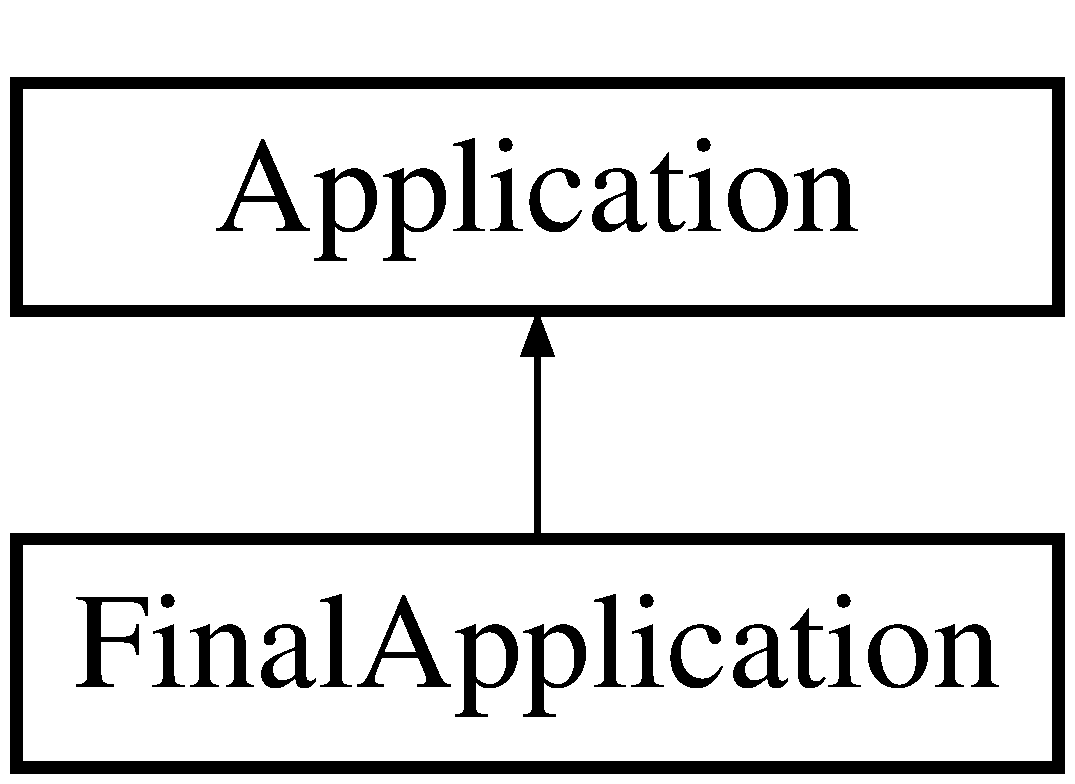
\includegraphics[height=2.000000cm]{class_final_application}
\end{center}
\end{figure}
\subsection*{Public Member Functions}
\begin{DoxyCompactItemize}
\item 
virtual void \hyperlink{class_final_application_acc4ece0398523f937ba601f006049efb}{on\-Run} () overridefinal
\begin{DoxyCompactList}\small\item\em Add a graph to the stats manager and update G\-U\-I. \end{DoxyCompactList}\item 
virtual void \hyperlink{class_final_application_a855c3f89d43c92e216a31d39d3ca3ce6}{on\-Event} (sf\-::\-Event event, sf\-::\-Render\-Window \&window) overridefinal
\begin{DoxyCompactList}\small\item\em Subclass can override this method to handle events. \end{DoxyCompactList}\item 
virtual void \hyperlink{class_final_application_afd3b9ffb92088376f27d72c12f90643d}{on\-Draw} (sf\-::\-Render\-Target \&target) overridefinal
\begin{DoxyCompactList}\small\item\em Subclass can override this method to draw their data in the simulation view. \end{DoxyCompactList}\end{DoxyCompactItemize}


\subsection{Member Function Documentation}
\hypertarget{class_final_application_afd3b9ffb92088376f27d72c12f90643d}{\index{Final\-Application@{Final\-Application}!on\-Draw@{on\-Draw}}
\index{on\-Draw@{on\-Draw}!FinalApplication@{Final\-Application}}
\subsubsection[{on\-Draw}]{\setlength{\rightskip}{0pt plus 5cm}void Final\-Application\-::on\-Draw (
\begin{DoxyParamCaption}
\item[{sf\-::\-Render\-Target \&}]{target}
\end{DoxyParamCaption}
)\hspace{0.3cm}{\ttfamily [final]}, {\ttfamily [override]}, {\ttfamily [virtual]}}}\label{class_final_application_afd3b9ffb92088376f27d72c12f90643d}


Subclass can override this method to draw their data in the simulation view. 

The default implementation does nothing. However, the env is always displayed first.


\begin{DoxyParams}{Parameters}
{\em target} & a render target \\
\hline
\end{DoxyParams}


Reimplemented from \hyperlink{class_application_ac35bfbd486eb47fdd2b5d731962c6724}{Application}.

\hypertarget{class_final_application_a855c3f89d43c92e216a31d39d3ca3ce6}{\index{Final\-Application@{Final\-Application}!on\-Event@{on\-Event}}
\index{on\-Event@{on\-Event}!FinalApplication@{Final\-Application}}
\subsubsection[{on\-Event}]{\setlength{\rightskip}{0pt plus 5cm}void Final\-Application\-::on\-Event (
\begin{DoxyParamCaption}
\item[{sf\-::\-Event}]{event, }
\item[{sf\-::\-Render\-Window \&}]{window}
\end{DoxyParamCaption}
)\hspace{0.3cm}{\ttfamily [final]}, {\ttfamily [override]}, {\ttfamily [virtual]}}}\label{class_final_application_a855c3f89d43c92e216a31d39d3ca3ce6}


Subclass can override this method to handle events. 

The default implementation does nothing.


\begin{DoxyParams}{Parameters}
{\em event} & an event \\
\hline
{\em window} & the window that emitted the event \\
\hline
\end{DoxyParams}


Reimplemented from \hyperlink{class_application_ae6ea28bafe249f7005aa143f36651342}{Application}.

\hypertarget{class_final_application_acc4ece0398523f937ba601f006049efb}{\index{Final\-Application@{Final\-Application}!on\-Run@{on\-Run}}
\index{on\-Run@{on\-Run}!FinalApplication@{Final\-Application}}
\subsubsection[{on\-Run}]{\setlength{\rightskip}{0pt plus 5cm}void Final\-Application\-::on\-Run (
\begin{DoxyParamCaption}
{}
\end{DoxyParamCaption}
)\hspace{0.3cm}{\ttfamily [final]}, {\ttfamily [override]}, {\ttfamily [virtual]}}}\label{class_final_application_acc4ece0398523f937ba601f006049efb}


Add a graph to the stats manager and update G\-U\-I. 


\begin{DoxyParams}{Parameters}
{\em title} & graph's title \\
\hline
{\em series} & series' title \\
\hline
{\em min} & y-\/axis\-: min value expected \\
\hline
{\em max} & y-\/axis\-: max value expected\\
\hline
\end{DoxyParams}
Called once before starting the main loop

By default nothing is done. 

Reimplemented from \hyperlink{class_application_af48ce2f324313699257c164dddb3b920}{Application}.



The documentation for this class was generated from the following files\-:\begin{DoxyCompactItemize}
\item 
/home/jbesson/myfiles/cpp/svprog/partie1/src/\hyperlink{_final_application_8hpp}{Final\-Application.\-hpp}\item 
/home/jbesson/myfiles/cpp/svprog/partie1/src/\hyperlink{_final_application_8cpp}{Final\-Application.\-cpp}\end{DoxyCompactItemize}

\hypertarget{classj_1_1_no_such_element}{\section{j\-:\-:No\-Such\-Element Class Reference}
\label{classj_1_1_no_such_element}\index{j\-::\-No\-Such\-Element@{j\-::\-No\-Such\-Element}}
}


{\ttfamily \#include $<$J\-S\-O\-N.\-hpp$>$}

Inheritance diagram for j\-:\-:No\-Such\-Element\-:\begin{figure}[H]
\begin{center}
\leavevmode
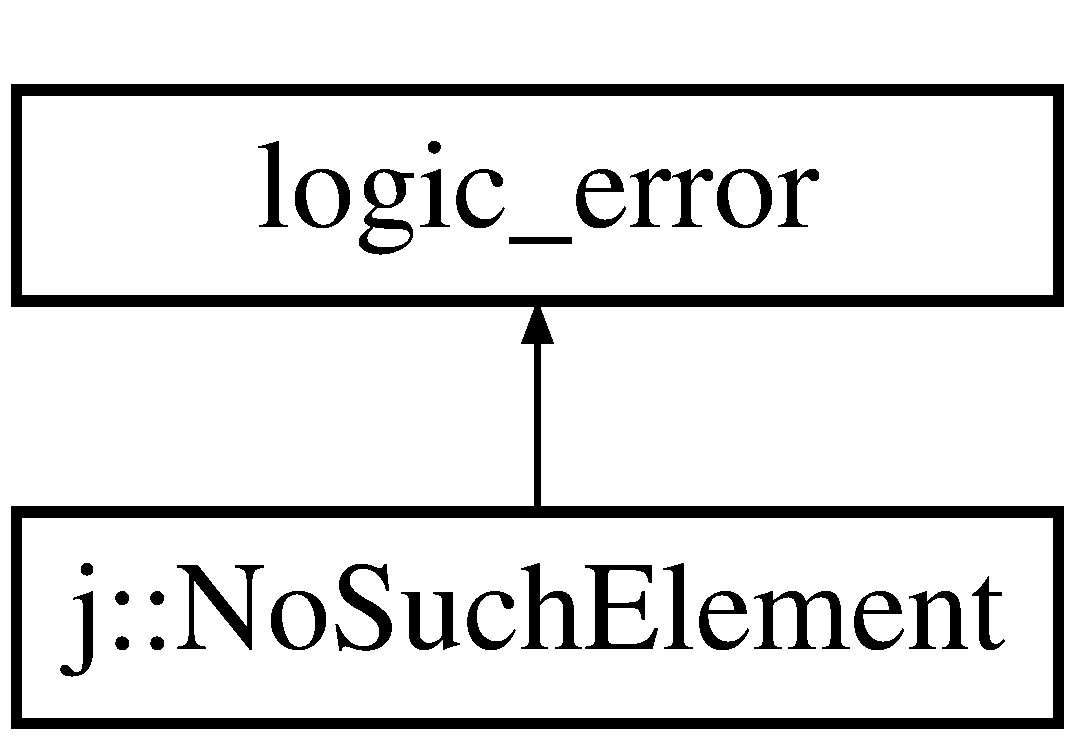
\includegraphics[height=2.000000cm]{classj_1_1_no_such_element}
\end{center}
\end{figure}
\subsection*{Public Member Functions}
\begin{DoxyCompactItemize}
\item 
\hyperlink{classj_1_1_no_such_element_a72a83b05d48e7d7805dc4cefaad325e3}{No\-Such\-Element} (std\-::string const \&elem)
\item 
\hyperlink{classj_1_1_no_such_element_a99542935049a656120e428d5611c28d8}{No\-Such\-Element} (std\-::size\-\_\-t index)
\end{DoxyCompactItemize}


\subsection{Constructor \& Destructor Documentation}
\hypertarget{classj_1_1_no_such_element_a72a83b05d48e7d7805dc4cefaad325e3}{\index{j\-::\-No\-Such\-Element@{j\-::\-No\-Such\-Element}!No\-Such\-Element@{No\-Such\-Element}}
\index{No\-Such\-Element@{No\-Such\-Element}!j::NoSuchElement@{j\-::\-No\-Such\-Element}}
\subsubsection[{No\-Such\-Element}]{\setlength{\rightskip}{0pt plus 5cm}j\-::\-No\-Such\-Element\-::\-No\-Such\-Element (
\begin{DoxyParamCaption}
\item[{std\-::string const \&}]{elem}
\end{DoxyParamCaption}
)}}\label{classj_1_1_no_such_element_a72a83b05d48e7d7805dc4cefaad325e3}
\hypertarget{classj_1_1_no_such_element_a99542935049a656120e428d5611c28d8}{\index{j\-::\-No\-Such\-Element@{j\-::\-No\-Such\-Element}!No\-Such\-Element@{No\-Such\-Element}}
\index{No\-Such\-Element@{No\-Such\-Element}!j::NoSuchElement@{j\-::\-No\-Such\-Element}}
\subsubsection[{No\-Such\-Element}]{\setlength{\rightskip}{0pt plus 5cm}j\-::\-No\-Such\-Element\-::\-No\-Such\-Element (
\begin{DoxyParamCaption}
\item[{std\-::size\-\_\-t}]{index}
\end{DoxyParamCaption}
)}}\label{classj_1_1_no_such_element_a99542935049a656120e428d5611c28d8}


The documentation for this class was generated from the following files\-:\begin{DoxyCompactItemize}
\item 
/home/jbesson/myfiles/cpp/svprog/partie1/src/\-J\-S\-O\-N/\hyperlink{_j_s_o_n_8hpp}{J\-S\-O\-N.\-hpp}\item 
/home/jbesson/myfiles/cpp/svprog/partie1/src/\-J\-S\-O\-N/\hyperlink{_j_s_o_n_8cpp}{J\-S\-O\-N.\-cpp}\end{DoxyCompactItemize}

\hypertarget{classj_1_1_no_such_file}{\section{j\-:\-:No\-Such\-File Class Reference}
\label{classj_1_1_no_such_file}\index{j\-::\-No\-Such\-File@{j\-::\-No\-Such\-File}}
}


{\ttfamily \#include $<$J\-S\-O\-N\-Serialiser.\-hpp$>$}

Inheritance diagram for j\-:\-:No\-Such\-File\-:\begin{figure}[H]
\begin{center}
\leavevmode
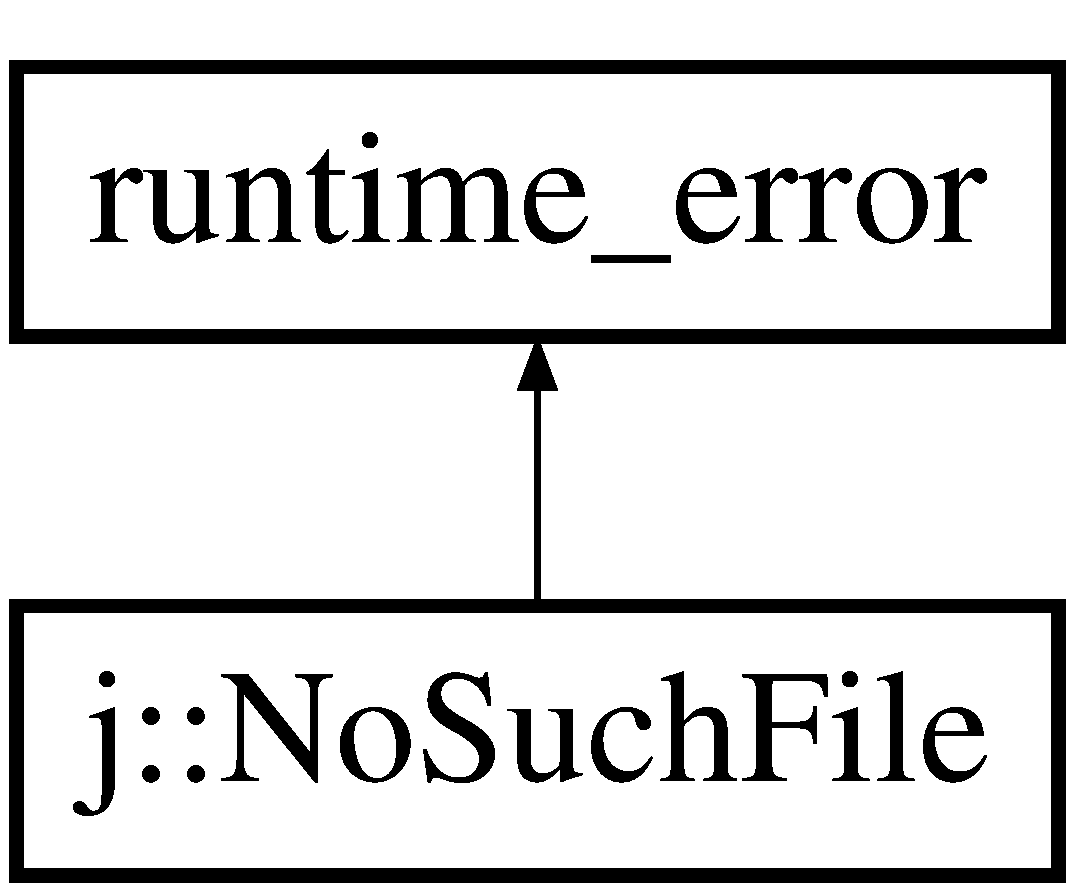
\includegraphics[height=2.000000cm]{classj_1_1_no_such_file}
\end{center}
\end{figure}
\subsection*{Public Member Functions}
\begin{DoxyCompactItemize}
\item 
\hyperlink{classj_1_1_no_such_file_a2fe02908b1e46fe8eaa0f4a597c76151}{No\-Such\-File} (std\-::string const \&msg)
\end{DoxyCompactItemize}


\subsection{Constructor \& Destructor Documentation}
\hypertarget{classj_1_1_no_such_file_a2fe02908b1e46fe8eaa0f4a597c76151}{\index{j\-::\-No\-Such\-File@{j\-::\-No\-Such\-File}!No\-Such\-File@{No\-Such\-File}}
\index{No\-Such\-File@{No\-Such\-File}!j::NoSuchFile@{j\-::\-No\-Such\-File}}
\subsubsection[{No\-Such\-File}]{\setlength{\rightskip}{0pt plus 5cm}j\-::\-No\-Such\-File\-::\-No\-Such\-File (
\begin{DoxyParamCaption}
\item[{std\-::string const \&}]{msg}
\end{DoxyParamCaption}
)}}\label{classj_1_1_no_such_file_a2fe02908b1e46fe8eaa0f4a597c76151}


The documentation for this class was generated from the following files\-:\begin{DoxyCompactItemize}
\item 
/home/jbesson/myfiles/cpp/svprog/partie1/src/\-J\-S\-O\-N/\hyperlink{_j_s_o_n_serialiser_8hpp}{J\-S\-O\-N\-Serialiser.\-hpp}\item 
/home/jbesson/myfiles/cpp/svprog/partie1/src/\-J\-S\-O\-N/\hyperlink{_j_s_o_n_serialiser_8cpp}{J\-S\-O\-N\-Serialiser.\-cpp}\end{DoxyCompactItemize}

\hypertarget{classj_1_1impl_1_1_number}{\section{j\-:\-:impl\-:\-:Number Class Reference}
\label{classj_1_1impl_1_1_number}\index{j\-::impl\-::\-Number@{j\-::impl\-::\-Number}}
}


{\ttfamily \#include $<$J\-S\-O\-N\-Impl.\-hpp$>$}

Inheritance diagram for j\-:\-:impl\-:\-:Number\-:\begin{figure}[H]
\begin{center}
\leavevmode
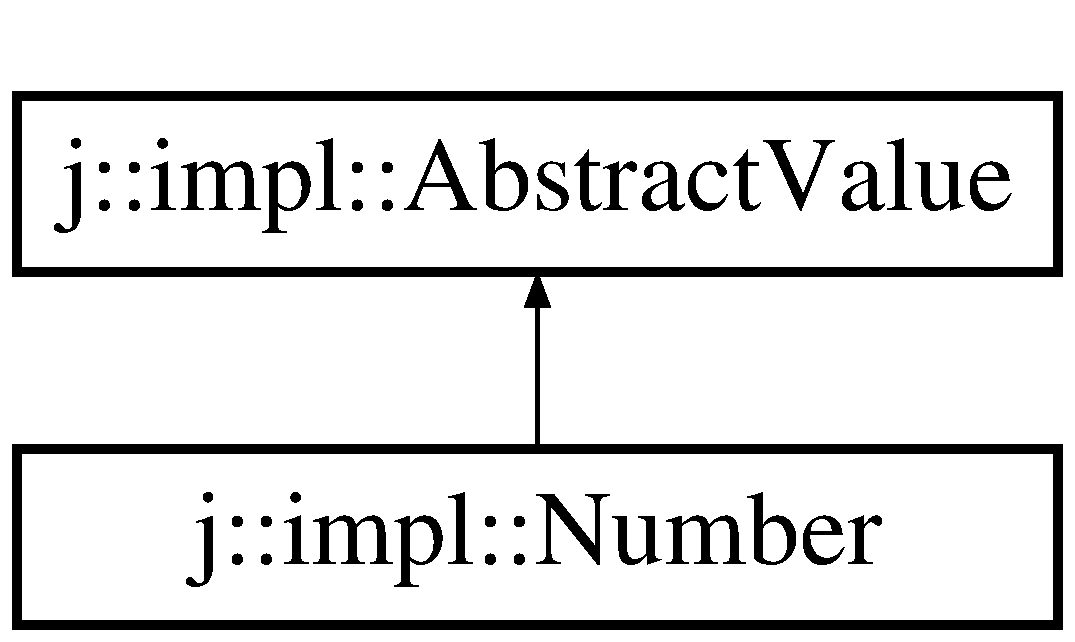
\includegraphics[height=2.000000cm]{classj_1_1impl_1_1_number}
\end{center}
\end{figure}
\subsection*{Public Member Functions}
\begin{DoxyCompactItemize}
\item 
\hyperlink{classj_1_1impl_1_1_number_a7a2374239a92ecb7e9c923ec675c46d1}{Number} (int integer)
\item 
\hyperlink{classj_1_1impl_1_1_number_a3d0ddcf35f9fafa40d92d353d8761f7c}{Number} (double real)
\item 
int \hyperlink{classj_1_1impl_1_1_number_a8f6a1bdd70886f790e2a3f285a96dd28}{to\-Int} () const 
\item 
double \hyperlink{classj_1_1impl_1_1_number_a434fd32607b9dd080e6c9ec26df6581f}{to\-Double} () const 
\item 
void \hyperlink{classj_1_1impl_1_1_number_af3b0824e2f419f9104c11a59f94914ee}{set} (int integer)
\item 
void \hyperlink{classj_1_1impl_1_1_number_a0ecf794de3e1b99548b8e094e0576297}{set} (double read)
\item 
bool \hyperlink{classj_1_1impl_1_1_number_a90888fbf7797a69fae21d3f6ad68fc84}{is\-Number} () const overridefinal
\item 
\hyperlink{classj_1_1impl_1_1_number}{Number} \& \hyperlink{classj_1_1impl_1_1_number_a86cf66c468eb3b75072bd431d8637529}{as\-Number} () overridefinal
\item 
\hyperlink{classj_1_1impl_1_1_number}{Number} const \& \hyperlink{classj_1_1impl_1_1_number_af72a6b872008d58ecd80547c89d9d355}{as\-Number} () const overridefinal
\item 
\hyperlink{classj_1_1impl_1_1_abstract_value}{Abstract\-Value} $\ast$ \hyperlink{classj_1_1impl_1_1_number_a4b48134b69e2fa6397477b1bd8334f68}{clone} () const overridefinal
\end{DoxyCompactItemize}
\subsection*{Private Attributes}
\begin{DoxyCompactItemize}
\item 
double \hyperlink{classj_1_1impl_1_1_number_a438e3d017fd472aea2d9e3bf2108aac7}{m\-Number}
\end{DoxyCompactItemize}


\subsection{Constructor \& Destructor Documentation}
\hypertarget{classj_1_1impl_1_1_number_a7a2374239a92ecb7e9c923ec675c46d1}{\index{j\-::impl\-::\-Number@{j\-::impl\-::\-Number}!Number@{Number}}
\index{Number@{Number}!j::impl::Number@{j\-::impl\-::\-Number}}
\subsubsection[{Number}]{\setlength{\rightskip}{0pt plus 5cm}j\-::impl\-::\-Number\-::\-Number (
\begin{DoxyParamCaption}
\item[{int}]{integer}
\end{DoxyParamCaption}
)}}\label{classj_1_1impl_1_1_number_a7a2374239a92ecb7e9c923ec675c46d1}
\hypertarget{classj_1_1impl_1_1_number_a3d0ddcf35f9fafa40d92d353d8761f7c}{\index{j\-::impl\-::\-Number@{j\-::impl\-::\-Number}!Number@{Number}}
\index{Number@{Number}!j::impl::Number@{j\-::impl\-::\-Number}}
\subsubsection[{Number}]{\setlength{\rightskip}{0pt plus 5cm}j\-::impl\-::\-Number\-::\-Number (
\begin{DoxyParamCaption}
\item[{double}]{real}
\end{DoxyParamCaption}
)}}\label{classj_1_1impl_1_1_number_a3d0ddcf35f9fafa40d92d353d8761f7c}


\subsection{Member Function Documentation}
\hypertarget{classj_1_1impl_1_1_number_a86cf66c468eb3b75072bd431d8637529}{\index{j\-::impl\-::\-Number@{j\-::impl\-::\-Number}!as\-Number@{as\-Number}}
\index{as\-Number@{as\-Number}!j::impl::Number@{j\-::impl\-::\-Number}}
\subsubsection[{as\-Number}]{\setlength{\rightskip}{0pt plus 5cm}{\bf Number} \& j\-::impl\-::\-Number\-::as\-Number (
\begin{DoxyParamCaption}
{}
\end{DoxyParamCaption}
)\hspace{0.3cm}{\ttfamily [final]}, {\ttfamily [override]}, {\ttfamily [virtual]}}}\label{classj_1_1impl_1_1_number_a86cf66c468eb3b75072bd431d8637529}


Reimplemented from \hyperlink{classj_1_1impl_1_1_abstract_value_a12d6d18e7b575da29ba587865ba06a9c}{j\-::impl\-::\-Abstract\-Value}.

\hypertarget{classj_1_1impl_1_1_number_af72a6b872008d58ecd80547c89d9d355}{\index{j\-::impl\-::\-Number@{j\-::impl\-::\-Number}!as\-Number@{as\-Number}}
\index{as\-Number@{as\-Number}!j::impl::Number@{j\-::impl\-::\-Number}}
\subsubsection[{as\-Number}]{\setlength{\rightskip}{0pt plus 5cm}{\bf Number} const \& j\-::impl\-::\-Number\-::as\-Number (
\begin{DoxyParamCaption}
{}
\end{DoxyParamCaption}
) const\hspace{0.3cm}{\ttfamily [final]}, {\ttfamily [override]}, {\ttfamily [virtual]}}}\label{classj_1_1impl_1_1_number_af72a6b872008d58ecd80547c89d9d355}


Reimplemented from \hyperlink{classj_1_1impl_1_1_abstract_value_a7b6246ea9bae83667abdbd7f58ece885}{j\-::impl\-::\-Abstract\-Value}.

\hypertarget{classj_1_1impl_1_1_number_a4b48134b69e2fa6397477b1bd8334f68}{\index{j\-::impl\-::\-Number@{j\-::impl\-::\-Number}!clone@{clone}}
\index{clone@{clone}!j::impl::Number@{j\-::impl\-::\-Number}}
\subsubsection[{clone}]{\setlength{\rightskip}{0pt plus 5cm}{\bf Abstract\-Value} $\ast$ j\-::impl\-::\-Number\-::clone (
\begin{DoxyParamCaption}
{}
\end{DoxyParamCaption}
) const\hspace{0.3cm}{\ttfamily [final]}, {\ttfamily [override]}, {\ttfamily [virtual]}}}\label{classj_1_1impl_1_1_number_a4b48134b69e2fa6397477b1bd8334f68}


Implements \hyperlink{classj_1_1impl_1_1_abstract_value_ac61a9aa4a4ecd3a309e8e274ac4b3dd2}{j\-::impl\-::\-Abstract\-Value}.

\hypertarget{classj_1_1impl_1_1_number_a90888fbf7797a69fae21d3f6ad68fc84}{\index{j\-::impl\-::\-Number@{j\-::impl\-::\-Number}!is\-Number@{is\-Number}}
\index{is\-Number@{is\-Number}!j::impl::Number@{j\-::impl\-::\-Number}}
\subsubsection[{is\-Number}]{\setlength{\rightskip}{0pt plus 5cm}bool j\-::impl\-::\-Number\-::is\-Number (
\begin{DoxyParamCaption}
{}
\end{DoxyParamCaption}
) const\hspace{0.3cm}{\ttfamily [final]}, {\ttfamily [override]}, {\ttfamily [virtual]}}}\label{classj_1_1impl_1_1_number_a90888fbf7797a69fae21d3f6ad68fc84}


Reimplemented from \hyperlink{classj_1_1impl_1_1_abstract_value_aab7be0e32dc9a488a9597d1fad5e84f5}{j\-::impl\-::\-Abstract\-Value}.

\hypertarget{classj_1_1impl_1_1_number_af3b0824e2f419f9104c11a59f94914ee}{\index{j\-::impl\-::\-Number@{j\-::impl\-::\-Number}!set@{set}}
\index{set@{set}!j::impl::Number@{j\-::impl\-::\-Number}}
\subsubsection[{set}]{\setlength{\rightskip}{0pt plus 5cm}void j\-::impl\-::\-Number\-::set (
\begin{DoxyParamCaption}
\item[{int}]{integer}
\end{DoxyParamCaption}
)}}\label{classj_1_1impl_1_1_number_af3b0824e2f419f9104c11a59f94914ee}
\hypertarget{classj_1_1impl_1_1_number_a0ecf794de3e1b99548b8e094e0576297}{\index{j\-::impl\-::\-Number@{j\-::impl\-::\-Number}!set@{set}}
\index{set@{set}!j::impl::Number@{j\-::impl\-::\-Number}}
\subsubsection[{set}]{\setlength{\rightskip}{0pt plus 5cm}void j\-::impl\-::\-Number\-::set (
\begin{DoxyParamCaption}
\item[{double}]{read}
\end{DoxyParamCaption}
)}}\label{classj_1_1impl_1_1_number_a0ecf794de3e1b99548b8e094e0576297}
\hypertarget{classj_1_1impl_1_1_number_a434fd32607b9dd080e6c9ec26df6581f}{\index{j\-::impl\-::\-Number@{j\-::impl\-::\-Number}!to\-Double@{to\-Double}}
\index{to\-Double@{to\-Double}!j::impl::Number@{j\-::impl\-::\-Number}}
\subsubsection[{to\-Double}]{\setlength{\rightskip}{0pt plus 5cm}double j\-::impl\-::\-Number\-::to\-Double (
\begin{DoxyParamCaption}
{}
\end{DoxyParamCaption}
) const}}\label{classj_1_1impl_1_1_number_a434fd32607b9dd080e6c9ec26df6581f}
\hypertarget{classj_1_1impl_1_1_number_a8f6a1bdd70886f790e2a3f285a96dd28}{\index{j\-::impl\-::\-Number@{j\-::impl\-::\-Number}!to\-Int@{to\-Int}}
\index{to\-Int@{to\-Int}!j::impl::Number@{j\-::impl\-::\-Number}}
\subsubsection[{to\-Int}]{\setlength{\rightskip}{0pt plus 5cm}int j\-::impl\-::\-Number\-::to\-Int (
\begin{DoxyParamCaption}
{}
\end{DoxyParamCaption}
) const}}\label{classj_1_1impl_1_1_number_a8f6a1bdd70886f790e2a3f285a96dd28}


\subsection{Member Data Documentation}
\hypertarget{classj_1_1impl_1_1_number_a438e3d017fd472aea2d9e3bf2108aac7}{\index{j\-::impl\-::\-Number@{j\-::impl\-::\-Number}!m\-Number@{m\-Number}}
\index{m\-Number@{m\-Number}!j::impl::Number@{j\-::impl\-::\-Number}}
\subsubsection[{m\-Number}]{\setlength{\rightskip}{0pt plus 5cm}double j\-::impl\-::\-Number\-::m\-Number\hspace{0.3cm}{\ttfamily [private]}}}\label{classj_1_1impl_1_1_number_a438e3d017fd472aea2d9e3bf2108aac7}


The documentation for this class was generated from the following files\-:\begin{DoxyCompactItemize}
\item 
/home/jbesson/myfiles/cpp/svprog/partie1/src/\-J\-S\-O\-N/\hyperlink{_j_s_o_n_impl_8hpp}{J\-S\-O\-N\-Impl.\-hpp}\item 
/home/jbesson/myfiles/cpp/svprog/partie1/src/\-J\-S\-O\-N/\hyperlink{_j_s_o_n_impl_8cpp}{J\-S\-O\-N\-Impl.\-cpp}\end{DoxyCompactItemize}

\hypertarget{classj_1_1impl_1_1_object}{\section{j\-:\-:impl\-:\-:Object Class Reference}
\label{classj_1_1impl_1_1_object}\index{j\-::impl\-::\-Object@{j\-::impl\-::\-Object}}
}


{\ttfamily \#include $<$J\-S\-O\-N\-Impl.\-hpp$>$}

Inheritance diagram for j\-:\-:impl\-:\-:Object\-:\begin{figure}[H]
\begin{center}
\leavevmode
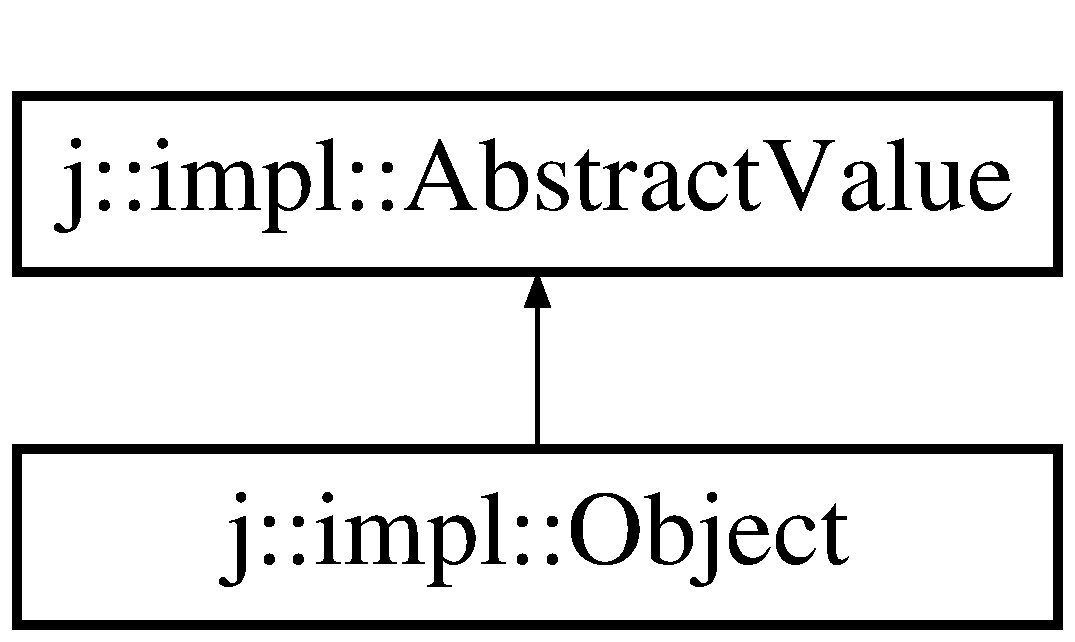
\includegraphics[height=2.000000cm]{classj_1_1impl_1_1_object}
\end{center}
\end{figure}
\subsection*{Public Member Functions}
\begin{DoxyCompactItemize}
\item 
bool \hyperlink{classj_1_1impl_1_1_object_ac66a504ae3a4592ad30176e3793bb90b}{operator==} (\hyperlink{classj_1_1impl_1_1_object}{Object} const \&other) const 
\item 
\hyperlink{classj_1_1_value}{Value} \& \hyperlink{classj_1_1impl_1_1_object_a2d132ef8f3e39ed354f6b2dcba3f6d45}{operator\mbox{[}$\,$\mbox{]}} (std\-::string const \&id)
\item 
\hyperlink{classj_1_1_value}{Value} const \& \hyperlink{classj_1_1impl_1_1_object_a2b56837fa3193cf76336216582383e9c}{operator\mbox{[}$\,$\mbox{]}} (std\-::string const \&id) const 
\item 
bool \hyperlink{classj_1_1impl_1_1_object_a1d870692cda482740f27d1ad877ee51b}{has\-Value} (std\-::string const \&id) const 
\item 
bool \hyperlink{classj_1_1impl_1_1_object_ac47b12fd0b97384c30394afd5225597f}{set} (std\-::string const \&id, \hyperlink{classj_1_1_value}{Value} const \&v)
\begin{DoxyCompactList}\small\item\em Update/insert a value. \end{DoxyCompactList}\item 
void \hyperlink{classj_1_1impl_1_1_object_a36d5a27d393f926a2fbeadb68f50b84a}{remove} (std\-::string const \&id)
\begin{DoxyCompactList}\small\item\em Remove the corresponding value from the \hyperlink{classj_1_1impl_1_1_object}{Object}. \end{DoxyCompactList}\item 
std\-::vector$<$ std\-::string $>$ \hyperlink{classj_1_1impl_1_1_object_ac43317d715c065f0e8b4ca40663a3341}{keys} () const 
\item 
bool \hyperlink{classj_1_1impl_1_1_object_a1a4c68884081496e04f4a84684980871}{is\-Object} () const overridefinal
\item 
\hyperlink{classj_1_1impl_1_1_object}{Object} \& \hyperlink{classj_1_1impl_1_1_object_aad1449adafdd83c980a03061ebf197c0}{as\-Object} () overridefinal
\item 
\hyperlink{classj_1_1impl_1_1_object}{Object} const \& \hyperlink{classj_1_1impl_1_1_object_a931f6aabe40406eb81106d0ec45ac1bd}{as\-Object} () const overridefinal
\item 
\hyperlink{classj_1_1impl_1_1_abstract_value}{Abstract\-Value} $\ast$ \hyperlink{classj_1_1impl_1_1_object_a7485852de6358152ec02e2e4023e3600}{clone} () const overridefinal
\end{DoxyCompactItemize}
\subsection*{Private Attributes}
\begin{DoxyCompactItemize}
\item 
std\-::unordered\-\_\-map\\*
$<$ std\-::string, std\-::unique\-\_\-ptr\\*
$<$ \hyperlink{classj_1_1_value}{Value} $>$ $>$ \hyperlink{classj_1_1impl_1_1_object_a43ac128967a0872b5edf707cd21c8676}{m\-Data}
\end{DoxyCompactItemize}


\subsection{Member Function Documentation}
\hypertarget{classj_1_1impl_1_1_object_aad1449adafdd83c980a03061ebf197c0}{\index{j\-::impl\-::\-Object@{j\-::impl\-::\-Object}!as\-Object@{as\-Object}}
\index{as\-Object@{as\-Object}!j::impl::Object@{j\-::impl\-::\-Object}}
\subsubsection[{as\-Object}]{\setlength{\rightskip}{0pt plus 5cm}{\bf Object} \& j\-::impl\-::\-Object\-::as\-Object (
\begin{DoxyParamCaption}
{}
\end{DoxyParamCaption}
)\hspace{0.3cm}{\ttfamily [final]}, {\ttfamily [override]}, {\ttfamily [virtual]}}}\label{classj_1_1impl_1_1_object_aad1449adafdd83c980a03061ebf197c0}


Reimplemented from \hyperlink{classj_1_1impl_1_1_abstract_value_ab692a8f260c4f0cf45ef0b7cc13ade66}{j\-::impl\-::\-Abstract\-Value}.

\hypertarget{classj_1_1impl_1_1_object_a931f6aabe40406eb81106d0ec45ac1bd}{\index{j\-::impl\-::\-Object@{j\-::impl\-::\-Object}!as\-Object@{as\-Object}}
\index{as\-Object@{as\-Object}!j::impl::Object@{j\-::impl\-::\-Object}}
\subsubsection[{as\-Object}]{\setlength{\rightskip}{0pt plus 5cm}{\bf Object} const \& j\-::impl\-::\-Object\-::as\-Object (
\begin{DoxyParamCaption}
{}
\end{DoxyParamCaption}
) const\hspace{0.3cm}{\ttfamily [final]}, {\ttfamily [override]}, {\ttfamily [virtual]}}}\label{classj_1_1impl_1_1_object_a931f6aabe40406eb81106d0ec45ac1bd}


Reimplemented from \hyperlink{classj_1_1impl_1_1_abstract_value_a99b098127ffda123446643bef12f574b}{j\-::impl\-::\-Abstract\-Value}.

\hypertarget{classj_1_1impl_1_1_object_a7485852de6358152ec02e2e4023e3600}{\index{j\-::impl\-::\-Object@{j\-::impl\-::\-Object}!clone@{clone}}
\index{clone@{clone}!j::impl::Object@{j\-::impl\-::\-Object}}
\subsubsection[{clone}]{\setlength{\rightskip}{0pt plus 5cm}{\bf Abstract\-Value} $\ast$ j\-::impl\-::\-Object\-::clone (
\begin{DoxyParamCaption}
{}
\end{DoxyParamCaption}
) const\hspace{0.3cm}{\ttfamily [final]}, {\ttfamily [override]}, {\ttfamily [virtual]}}}\label{classj_1_1impl_1_1_object_a7485852de6358152ec02e2e4023e3600}


Implements \hyperlink{classj_1_1impl_1_1_abstract_value_ac61a9aa4a4ecd3a309e8e274ac4b3dd2}{j\-::impl\-::\-Abstract\-Value}.

\hypertarget{classj_1_1impl_1_1_object_a1d870692cda482740f27d1ad877ee51b}{\index{j\-::impl\-::\-Object@{j\-::impl\-::\-Object}!has\-Value@{has\-Value}}
\index{has\-Value@{has\-Value}!j::impl::Object@{j\-::impl\-::\-Object}}
\subsubsection[{has\-Value}]{\setlength{\rightskip}{0pt plus 5cm}bool j\-::impl\-::\-Object\-::has\-Value (
\begin{DoxyParamCaption}
\item[{std\-::string const \&}]{id}
\end{DoxyParamCaption}
) const}}\label{classj_1_1impl_1_1_object_a1d870692cda482740f27d1ad877ee51b}
\hypertarget{classj_1_1impl_1_1_object_a1a4c68884081496e04f4a84684980871}{\index{j\-::impl\-::\-Object@{j\-::impl\-::\-Object}!is\-Object@{is\-Object}}
\index{is\-Object@{is\-Object}!j::impl::Object@{j\-::impl\-::\-Object}}
\subsubsection[{is\-Object}]{\setlength{\rightskip}{0pt plus 5cm}bool j\-::impl\-::\-Object\-::is\-Object (
\begin{DoxyParamCaption}
{}
\end{DoxyParamCaption}
) const\hspace{0.3cm}{\ttfamily [final]}, {\ttfamily [override]}, {\ttfamily [virtual]}}}\label{classj_1_1impl_1_1_object_a1a4c68884081496e04f4a84684980871}


Reimplemented from \hyperlink{classj_1_1impl_1_1_abstract_value_a62b0b78a969ba3d8ea426e46c96c2517}{j\-::impl\-::\-Abstract\-Value}.

\hypertarget{classj_1_1impl_1_1_object_ac43317d715c065f0e8b4ca40663a3341}{\index{j\-::impl\-::\-Object@{j\-::impl\-::\-Object}!keys@{keys}}
\index{keys@{keys}!j::impl::Object@{j\-::impl\-::\-Object}}
\subsubsection[{keys}]{\setlength{\rightskip}{0pt plus 5cm}std\-::vector$<$ std\-::string $>$ j\-::impl\-::\-Object\-::keys (
\begin{DoxyParamCaption}
{}
\end{DoxyParamCaption}
) const}}\label{classj_1_1impl_1_1_object_ac43317d715c065f0e8b4ca40663a3341}
\hypertarget{classj_1_1impl_1_1_object_ac66a504ae3a4592ad30176e3793bb90b}{\index{j\-::impl\-::\-Object@{j\-::impl\-::\-Object}!operator==@{operator==}}
\index{operator==@{operator==}!j::impl::Object@{j\-::impl\-::\-Object}}
\subsubsection[{operator==}]{\setlength{\rightskip}{0pt plus 5cm}bool j\-::impl\-::\-Object\-::operator== (
\begin{DoxyParamCaption}
\item[{{\bf Object} const \&}]{other}
\end{DoxyParamCaption}
) const}}\label{classj_1_1impl_1_1_object_ac66a504ae3a4592ad30176e3793bb90b}
\hypertarget{classj_1_1impl_1_1_object_a2d132ef8f3e39ed354f6b2dcba3f6d45}{\index{j\-::impl\-::\-Object@{j\-::impl\-::\-Object}!operator\mbox{[}$\,$\mbox{]}@{operator[]}}
\index{operator\mbox{[}$\,$\mbox{]}@{operator[]}!j::impl::Object@{j\-::impl\-::\-Object}}
\subsubsection[{operator[]}]{\setlength{\rightskip}{0pt plus 5cm}{\bf Value} \& j\-::impl\-::\-Object\-::operator\mbox{[}$\,$\mbox{]} (
\begin{DoxyParamCaption}
\item[{std\-::string const \&}]{id}
\end{DoxyParamCaption}
)}}\label{classj_1_1impl_1_1_object_a2d132ef8f3e39ed354f6b2dcba3f6d45}
\hypertarget{classj_1_1impl_1_1_object_a2b56837fa3193cf76336216582383e9c}{\index{j\-::impl\-::\-Object@{j\-::impl\-::\-Object}!operator\mbox{[}$\,$\mbox{]}@{operator[]}}
\index{operator\mbox{[}$\,$\mbox{]}@{operator[]}!j::impl::Object@{j\-::impl\-::\-Object}}
\subsubsection[{operator[]}]{\setlength{\rightskip}{0pt plus 5cm}{\bf Value} const \& j\-::impl\-::\-Object\-::operator\mbox{[}$\,$\mbox{]} (
\begin{DoxyParamCaption}
\item[{std\-::string const \&}]{id}
\end{DoxyParamCaption}
) const}}\label{classj_1_1impl_1_1_object_a2b56837fa3193cf76336216582383e9c}
\hypertarget{classj_1_1impl_1_1_object_a36d5a27d393f926a2fbeadb68f50b84a}{\index{j\-::impl\-::\-Object@{j\-::impl\-::\-Object}!remove@{remove}}
\index{remove@{remove}!j::impl::Object@{j\-::impl\-::\-Object}}
\subsubsection[{remove}]{\setlength{\rightskip}{0pt plus 5cm}void j\-::impl\-::\-Object\-::remove (
\begin{DoxyParamCaption}
\item[{std\-::string const \&}]{id}
\end{DoxyParamCaption}
)}}\label{classj_1_1impl_1_1_object_a36d5a27d393f926a2fbeadb68f50b84a}


Remove the corresponding value from the \hyperlink{classj_1_1impl_1_1_object}{Object}. 


\begin{DoxyExceptions}{Exceptions}
{\em \hyperlink{classj_1_1_no_such_element}{No\-Such\-Element}} & when the id is not present in the \hyperlink{classj_1_1impl_1_1_object}{Object}\\
\hline
\end{DoxyExceptions}

\begin{DoxyParams}{Parameters}
{\em id} & an id \\
\hline
\end{DoxyParams}
\hypertarget{classj_1_1impl_1_1_object_ac47b12fd0b97384c30394afd5225597f}{\index{j\-::impl\-::\-Object@{j\-::impl\-::\-Object}!set@{set}}
\index{set@{set}!j::impl::Object@{j\-::impl\-::\-Object}}
\subsubsection[{set}]{\setlength{\rightskip}{0pt plus 5cm}bool j\-::impl\-::\-Object\-::set (
\begin{DoxyParamCaption}
\item[{std\-::string const \&}]{id, }
\item[{{\bf Value} const \&}]{v}
\end{DoxyParamCaption}
)}}\label{classj_1_1impl_1_1_object_ac47b12fd0b97384c30394afd5225597f}


Update/insert a value. 


\begin{DoxyParams}{Parameters}
{\em id} & an identifier for the value \\
\hline
{\em v} & a value\\
\hline
\end{DoxyParams}
\begin{DoxyReturn}{Returns}
true if there was no such value before the insertion, false otherwise 
\end{DoxyReturn}


\subsection{Member Data Documentation}
\hypertarget{classj_1_1impl_1_1_object_a43ac128967a0872b5edf707cd21c8676}{\index{j\-::impl\-::\-Object@{j\-::impl\-::\-Object}!m\-Data@{m\-Data}}
\index{m\-Data@{m\-Data}!j::impl::Object@{j\-::impl\-::\-Object}}
\subsubsection[{m\-Data}]{\setlength{\rightskip}{0pt plus 5cm}std\-::unordered\-\_\-map$<$std\-::string, std\-::unique\-\_\-ptr$<${\bf Value}$>$ $>$ j\-::impl\-::\-Object\-::m\-Data\hspace{0.3cm}{\ttfamily [private]}}}\label{classj_1_1impl_1_1_object_a43ac128967a0872b5edf707cd21c8676}


The documentation for this class was generated from the following files\-:\begin{DoxyCompactItemize}
\item 
/home/jbesson/myfiles/cpp/svprog/partie1/src/\-J\-S\-O\-N/\hyperlink{_j_s_o_n_impl_8hpp}{J\-S\-O\-N\-Impl.\-hpp}\item 
/home/jbesson/myfiles/cpp/svprog/partie1/src/\-J\-S\-O\-N/\hyperlink{_j_s_o_n_impl_8cpp}{J\-S\-O\-N\-Impl.\-cpp}\end{DoxyCompactItemize}

\hypertarget{structj_1_1_value_1_1_object_tag}{\section{j\-:\-:Value\-:\-:Object\-Tag Struct Reference}
\label{structj_1_1_value_1_1_object_tag}\index{j\-::\-Value\-::\-Object\-Tag@{j\-::\-Value\-::\-Object\-Tag}}
}


{\ttfamily \#include $<$J\-S\-O\-N.\-hpp$>$}



The documentation for this struct was generated from the following file\-:\begin{DoxyCompactItemize}
\item 
/home/jbesson/myfiles/cpp/svprog/partie1/src/\-J\-S\-O\-N/\hyperlink{_j_s_o_n_8hpp}{J\-S\-O\-N.\-hpp}\end{DoxyCompactItemize}

\hypertarget{classj_1_1impl_1_1_string}{\section{j\-:\-:impl\-:\-:String Class Reference}
\label{classj_1_1impl_1_1_string}\index{j\-::impl\-::\-String@{j\-::impl\-::\-String}}
}


{\ttfamily \#include $<$J\-S\-O\-N\-Impl.\-hpp$>$}

Inheritance diagram for j\-:\-:impl\-:\-:String\-:\begin{figure}[H]
\begin{center}
\leavevmode
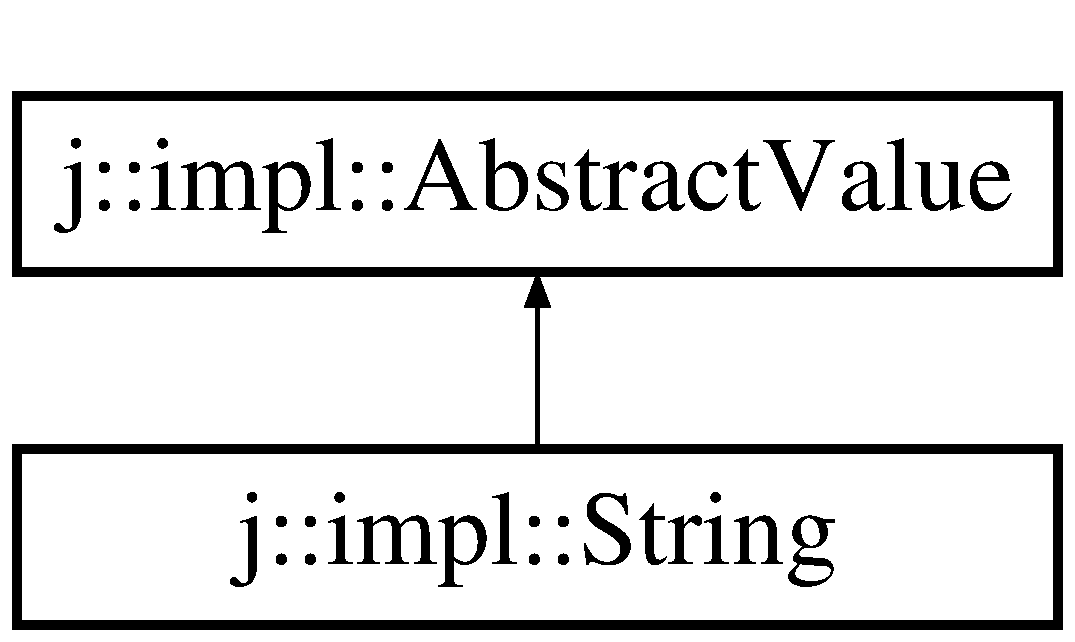
\includegraphics[height=2.000000cm]{classj_1_1impl_1_1_string}
\end{center}
\end{figure}
\subsection*{Public Member Functions}
\begin{DoxyCompactItemize}
\item 
\hyperlink{classj_1_1impl_1_1_string_a4892fe3f3e362666d1d56eb6ce9b76e7}{String} (std\-::string const \&str)
\item 
std\-::string \hyperlink{classj_1_1impl_1_1_string_aeaa593c84a7cac7074aae01198a68c5a}{to\-Raw\-String} () const 
\item 
void \hyperlink{classj_1_1impl_1_1_string_ab3f3a249161503f7a32853bfb9517d60}{set} (std\-::string const \&str)
\item 
bool \hyperlink{classj_1_1impl_1_1_string_a6ca9214f2d17ebfd0375b4c24e233c89}{is\-String} () const overridefinal
\item 
\hyperlink{classj_1_1impl_1_1_string}{String} \& \hyperlink{classj_1_1impl_1_1_string_a0a9ce87a737e81d5a035fa756d7ecd60}{as\-String} () overridefinal
\item 
\hyperlink{classj_1_1impl_1_1_string}{String} const \& \hyperlink{classj_1_1impl_1_1_string_aaa33cceb60b66372afe727dba5621315}{as\-String} () const overridefinal
\item 
\hyperlink{classj_1_1impl_1_1_abstract_value}{Abstract\-Value} $\ast$ \hyperlink{classj_1_1impl_1_1_string_ac449f19ca6504c13249db0c035444179}{clone} () const overridefinal
\end{DoxyCompactItemize}
\subsection*{Private Attributes}
\begin{DoxyCompactItemize}
\item 
std\-::string \hyperlink{classj_1_1impl_1_1_string_ad8b558370f1d17a6d17e25430049447e}{m\-String}
\end{DoxyCompactItemize}


\subsection{Constructor \& Destructor Documentation}
\hypertarget{classj_1_1impl_1_1_string_a4892fe3f3e362666d1d56eb6ce9b76e7}{\index{j\-::impl\-::\-String@{j\-::impl\-::\-String}!String@{String}}
\index{String@{String}!j::impl::String@{j\-::impl\-::\-String}}
\subsubsection[{String}]{\setlength{\rightskip}{0pt plus 5cm}j\-::impl\-::\-String\-::\-String (
\begin{DoxyParamCaption}
\item[{std\-::string const \&}]{str}
\end{DoxyParamCaption}
)}}\label{classj_1_1impl_1_1_string_a4892fe3f3e362666d1d56eb6ce9b76e7}


\subsection{Member Function Documentation}
\hypertarget{classj_1_1impl_1_1_string_a0a9ce87a737e81d5a035fa756d7ecd60}{\index{j\-::impl\-::\-String@{j\-::impl\-::\-String}!as\-String@{as\-String}}
\index{as\-String@{as\-String}!j::impl::String@{j\-::impl\-::\-String}}
\subsubsection[{as\-String}]{\setlength{\rightskip}{0pt plus 5cm}{\bf String} \& j\-::impl\-::\-String\-::as\-String (
\begin{DoxyParamCaption}
{}
\end{DoxyParamCaption}
)\hspace{0.3cm}{\ttfamily [final]}, {\ttfamily [override]}, {\ttfamily [virtual]}}}\label{classj_1_1impl_1_1_string_a0a9ce87a737e81d5a035fa756d7ecd60}


Reimplemented from \hyperlink{classj_1_1impl_1_1_abstract_value_a7bbc123a13e953d51789f65d8e974aa1}{j\-::impl\-::\-Abstract\-Value}.

\hypertarget{classj_1_1impl_1_1_string_aaa33cceb60b66372afe727dba5621315}{\index{j\-::impl\-::\-String@{j\-::impl\-::\-String}!as\-String@{as\-String}}
\index{as\-String@{as\-String}!j::impl::String@{j\-::impl\-::\-String}}
\subsubsection[{as\-String}]{\setlength{\rightskip}{0pt plus 5cm}{\bf String} const \& j\-::impl\-::\-String\-::as\-String (
\begin{DoxyParamCaption}
{}
\end{DoxyParamCaption}
) const\hspace{0.3cm}{\ttfamily [final]}, {\ttfamily [override]}, {\ttfamily [virtual]}}}\label{classj_1_1impl_1_1_string_aaa33cceb60b66372afe727dba5621315}


Reimplemented from \hyperlink{classj_1_1impl_1_1_abstract_value_a93ea458da59b4a9cab2cc7c359792105}{j\-::impl\-::\-Abstract\-Value}.

\hypertarget{classj_1_1impl_1_1_string_ac449f19ca6504c13249db0c035444179}{\index{j\-::impl\-::\-String@{j\-::impl\-::\-String}!clone@{clone}}
\index{clone@{clone}!j::impl::String@{j\-::impl\-::\-String}}
\subsubsection[{clone}]{\setlength{\rightskip}{0pt plus 5cm}{\bf Abstract\-Value} $\ast$ j\-::impl\-::\-String\-::clone (
\begin{DoxyParamCaption}
{}
\end{DoxyParamCaption}
) const\hspace{0.3cm}{\ttfamily [final]}, {\ttfamily [override]}, {\ttfamily [virtual]}}}\label{classj_1_1impl_1_1_string_ac449f19ca6504c13249db0c035444179}


Implements \hyperlink{classj_1_1impl_1_1_abstract_value_ac61a9aa4a4ecd3a309e8e274ac4b3dd2}{j\-::impl\-::\-Abstract\-Value}.

\hypertarget{classj_1_1impl_1_1_string_a6ca9214f2d17ebfd0375b4c24e233c89}{\index{j\-::impl\-::\-String@{j\-::impl\-::\-String}!is\-String@{is\-String}}
\index{is\-String@{is\-String}!j::impl::String@{j\-::impl\-::\-String}}
\subsubsection[{is\-String}]{\setlength{\rightskip}{0pt plus 5cm}bool j\-::impl\-::\-String\-::is\-String (
\begin{DoxyParamCaption}
{}
\end{DoxyParamCaption}
) const\hspace{0.3cm}{\ttfamily [final]}, {\ttfamily [override]}, {\ttfamily [virtual]}}}\label{classj_1_1impl_1_1_string_a6ca9214f2d17ebfd0375b4c24e233c89}


Reimplemented from \hyperlink{classj_1_1impl_1_1_abstract_value_ac931756f6157e90b6f824fb4ae9e6ee2}{j\-::impl\-::\-Abstract\-Value}.

\hypertarget{classj_1_1impl_1_1_string_ab3f3a249161503f7a32853bfb9517d60}{\index{j\-::impl\-::\-String@{j\-::impl\-::\-String}!set@{set}}
\index{set@{set}!j::impl::String@{j\-::impl\-::\-String}}
\subsubsection[{set}]{\setlength{\rightskip}{0pt plus 5cm}void j\-::impl\-::\-String\-::set (
\begin{DoxyParamCaption}
\item[{std\-::string const \&}]{str}
\end{DoxyParamCaption}
)}}\label{classj_1_1impl_1_1_string_ab3f3a249161503f7a32853bfb9517d60}
\hypertarget{classj_1_1impl_1_1_string_aeaa593c84a7cac7074aae01198a68c5a}{\index{j\-::impl\-::\-String@{j\-::impl\-::\-String}!to\-Raw\-String@{to\-Raw\-String}}
\index{to\-Raw\-String@{to\-Raw\-String}!j::impl::String@{j\-::impl\-::\-String}}
\subsubsection[{to\-Raw\-String}]{\setlength{\rightskip}{0pt plus 5cm}std\-::string j\-::impl\-::\-String\-::to\-Raw\-String (
\begin{DoxyParamCaption}
{}
\end{DoxyParamCaption}
) const}}\label{classj_1_1impl_1_1_string_aeaa593c84a7cac7074aae01198a68c5a}


\subsection{Member Data Documentation}
\hypertarget{classj_1_1impl_1_1_string_ad8b558370f1d17a6d17e25430049447e}{\index{j\-::impl\-::\-String@{j\-::impl\-::\-String}!m\-String@{m\-String}}
\index{m\-String@{m\-String}!j::impl::String@{j\-::impl\-::\-String}}
\subsubsection[{m\-String}]{\setlength{\rightskip}{0pt plus 5cm}std\-::string j\-::impl\-::\-String\-::m\-String\hspace{0.3cm}{\ttfamily [private]}}}\label{classj_1_1impl_1_1_string_ad8b558370f1d17a6d17e25430049447e}


The documentation for this class was generated from the following files\-:\begin{DoxyCompactItemize}
\item 
/home/jbesson/myfiles/cpp/svprog/partie1/src/\-J\-S\-O\-N/\hyperlink{_j_s_o_n_impl_8hpp}{J\-S\-O\-N\-Impl.\-hpp}\item 
/home/jbesson/myfiles/cpp/svprog/partie1/src/\-J\-S\-O\-N/\hyperlink{_j_s_o_n_impl_8cpp}{J\-S\-O\-N\-Impl.\-cpp}\end{DoxyCompactItemize}

\hypertarget{class_updatable}{\section{Updatable Class Reference}
\label{class_updatable}\index{Updatable@{Updatable}}
}


Represents an entity that evolves with time.  




{\ttfamily \#include $<$Updatable.\-hpp$>$}

\subsection*{Public Member Functions}
\begin{DoxyCompactItemize}
\item 
virtual \hyperlink{class_updatable_a8f2caa68bd46bfe52bf96b6af9a9d640}{$\sim$\-Updatable} ()=default
\item 
virtual void \hyperlink{class_updatable_acc8fbddaa1248aacd62ebef9f8dab513}{update} (sf\-::\-Time dt)=0
\end{DoxyCompactItemize}


\subsection{Detailed Description}
Represents an entity that evolves with time. 

\subsection{Constructor \& Destructor Documentation}
\hypertarget{class_updatable_a8f2caa68bd46bfe52bf96b6af9a9d640}{\index{Updatable@{Updatable}!$\sim$\-Updatable@{$\sim$\-Updatable}}
\index{$\sim$\-Updatable@{$\sim$\-Updatable}!Updatable@{Updatable}}
\subsubsection[{$\sim$\-Updatable}]{\setlength{\rightskip}{0pt plus 5cm}virtual Updatable\-::$\sim$\-Updatable (
\begin{DoxyParamCaption}
{}
\end{DoxyParamCaption}
)\hspace{0.3cm}{\ttfamily [virtual]}, {\ttfamily [default]}}}\label{class_updatable_a8f2caa68bd46bfe52bf96b6af9a9d640}


\subsection{Member Function Documentation}
\hypertarget{class_updatable_acc8fbddaa1248aacd62ebef9f8dab513}{\index{Updatable@{Updatable}!update@{update}}
\index{update@{update}!Updatable@{Updatable}}
\subsubsection[{update}]{\setlength{\rightskip}{0pt plus 5cm}virtual void Updatable\-::update (
\begin{DoxyParamCaption}
\item[{sf\-::\-Time}]{dt}
\end{DoxyParamCaption}
)\hspace{0.3cm}{\ttfamily [pure virtual]}}}\label{class_updatable_acc8fbddaa1248aacd62ebef9f8dab513}


The documentation for this class was generated from the following file\-:\begin{DoxyCompactItemize}
\item 
/home/jbesson/myfiles/cpp/svprog/partie1/src/\-Interface/\hyperlink{_updatable_8hpp}{Updatable.\-hpp}\end{DoxyCompactItemize}

\hypertarget{classj_1_1_value}{\section{j\-:\-:Value Class Reference}
\label{classj_1_1_value}\index{j\-::\-Value@{j\-::\-Value}}
}


{\ttfamily \#include $<$J\-S\-O\-N.\-hpp$>$}

\subsection*{Classes}
\begin{DoxyCompactItemize}
\item 
struct \hyperlink{structj_1_1_value_1_1_array_tag}{Array\-Tag}
\item 
struct \hyperlink{structj_1_1_value_1_1_object_tag}{Object\-Tag}
\end{DoxyCompactItemize}
\subsection*{Public Member Functions}
\begin{DoxyCompactItemize}
\item 
\hyperlink{classj_1_1_value_a9281dfcb57d331813484c0fb2926954e}{Value} (\hyperlink{classj_1_1_value}{Value} const \&other)
\item 
\hyperlink{classj_1_1_value}{Value} \& \hyperlink{classj_1_1_value_ac6f7f01183a7309a5290397f4b981a74}{operator=} (\hyperlink{classj_1_1_value}{Value} const \&other)
\item 
bool \hyperlink{classj_1_1_value_a6afbb65a1bad5ab74846b8ddc4facb1e}{is\-String} () const 
\item 
bool \hyperlink{classj_1_1_value_affbf70f3c3c1b9248c8a779a36b05d7e}{is\-Number} () const 
\item 
bool \hyperlink{classj_1_1_value_abf425e0f735047a53e9c01cb27047f48}{is\-Boolean} () const 
\item 
bool \hyperlink{classj_1_1_value_af9028d620fe389617b2d44ee7f278456}{is\-Object} () const 
\item 
bool \hyperlink{classj_1_1_value_adbbc6726787797844fef035236b90397}{is\-Array} () const 
\item 
std\-::string \hyperlink{classj_1_1_value_aa64c83251f06e39892c2d30ef9420b11}{to\-String} () const 
\item 
int \hyperlink{classj_1_1_value_a25ee203bd5870a7f22ee808dfe511fed}{to\-Int} () const 
\item 
double \hyperlink{classj_1_1_value_a2eaf6897ca4b7d931b248027645b8b0a}{to\-Double} () const 
\item 
bool \hyperlink{classj_1_1_value_abe6657b7f2985d668923d89ce97b825f}{to\-Bool} () const 
\item 
\hyperlink{classj_1_1_value}{Value} \& \hyperlink{classj_1_1_value_a1d7bd6425d8e824c2fb5eba9ae300f35}{operator\mbox{[}$\,$\mbox{]}} (std\-::string const \&id)
\item 
\hyperlink{classj_1_1_value}{Value} const \& \hyperlink{classj_1_1_value_a456ddc23a8788bc3707fd99d8654da1d}{operator\mbox{[}$\,$\mbox{]}} (std\-::string const \&id) const 
\item 
bool \hyperlink{classj_1_1_value_a003ec951adeedf5eae2307c2ef81e6b5}{has\-Value} (std\-::string const \&id) const 
\item 
bool \hyperlink{classj_1_1_value_acb7200e71d27f9271748d478e4b9969b}{set} (std\-::string const \&id, \hyperlink{classj_1_1_value}{Value} const \&v)
\item 
void \hyperlink{classj_1_1_value_a590c1697a143f82b3ba7625ee5fedd89}{remove} (std\-::string const \&id)
\item 
std\-::vector$<$ std\-::string $>$ \hyperlink{classj_1_1_value_a048c775e05118ea81ef1465589f90e63}{keys} () const 
\item 
\hyperlink{classj_1_1_value}{Value} \& \hyperlink{classj_1_1_value_a1b61a09b9fccc9b5356a5f30ebce6eb4}{operator\mbox{[}$\,$\mbox{]}} (std\-::size\-\_\-t i)
\item 
\hyperlink{classj_1_1_value}{Value} const \& \hyperlink{classj_1_1_value_aff7ae837a3da198446bf66df3c61f588}{operator\mbox{[}$\,$\mbox{]}} (std\-::size\-\_\-t i) const 
\item 
std\-::size\-\_\-t \hyperlink{classj_1_1_value_a33a99eef89c693d834e391dc8b7aec98}{size} () const 
\item 
void \hyperlink{classj_1_1_value_abcebda8aa6c8e2f58a91c22a8a07e680}{add} (\hyperlink{classj_1_1_value}{Value} const \&v)
\item 
void \hyperlink{classj_1_1_value_ab59e64a499c44665ef338056f46ecaad}{remove} (std\-::size\-\_\-t i)
\end{DoxyCompactItemize}
\subsection*{Protected Member Functions}
\begin{DoxyCompactItemize}
\item 
\hyperlink{classj_1_1_value_a90225534bf6d37de16adb1f1d10bfc64}{Value} (std\-::string const \&str)
\item 
\hyperlink{classj_1_1_value_af9019aad3e70ff3d91517360157040ed}{Value} (int num)
\item 
\hyperlink{classj_1_1_value_a8662002a5abad2e1c2620ddeb20dcfb8}{Value} (double num)
\item 
\hyperlink{classj_1_1_value_ad84533b7a8c5995e6bb277211e679fba}{Value} (bool \hyperlink{classj_1_1_value_ac55f3b10c1cdf64e972218bfe8a4a765}{boolean})
\item 
\hyperlink{classj_1_1_value_af49742c0a6be2a6041168f724aaa0ed5}{Value} (\hyperlink{structj_1_1_value_1_1_object_tag}{Object\-Tag})
\item 
\hyperlink{classj_1_1_value_a23f291de964d8e8e96f53ef42bca5801}{Value} (\hyperlink{structj_1_1_value_1_1_array_tag}{Array\-Tag})
\item 
\hyperlink{classj_1_1_value_a8e4003dd8e5ede9ccc1c6ac0508d3889}{Value} ()=delete
\end{DoxyCompactItemize}
\subsection*{Static Protected Attributes}
\begin{DoxyCompactItemize}
\item 
static constexpr struct \\*
\hyperlink{structj_1_1_value_1_1_object_tag}{j\-::\-Value\-::\-Object\-Tag} \hyperlink{classj_1_1_value_adb703d34b8b58a1a301183d092b86a16}{object\-Tag}
\item 
static constexpr struct \\*
\hyperlink{structj_1_1_value_1_1_array_tag}{j\-::\-Value\-::\-Array\-Tag} \hyperlink{classj_1_1_value_a222ab93e1ee2faeb71d53d98cf3fda2a}{array\-Tag}
\end{DoxyCompactItemize}
\subsection*{Private Attributes}
\begin{DoxyCompactItemize}
\item 
std\-::unique\-\_\-ptr\\*
$<$ \hyperlink{classj_1_1impl_1_1_abstract_value}{impl\-::\-Abstract\-Value} $>$ \hyperlink{classj_1_1_value_a07b659b8454529ba651033e32a203540}{m\-Impl}
\end{DoxyCompactItemize}
\subsection*{Friends}
\begin{DoxyCompactItemize}
\item 
\hyperlink{classj_1_1_value}{Value} \hyperlink{classj_1_1_value_a708a58b570f1bc42bb0fcf3468ea9ab8}{string} (std\-::string const \&str)
\item 
\hyperlink{classj_1_1_value}{Value} \hyperlink{classj_1_1_value_ac0ea80516ee9924893236d06b3e6bce1}{number} (int num)
\item 
\hyperlink{classj_1_1_value}{Value} \hyperlink{classj_1_1_value_a8db9f9d7dced9b3f7e0d02428b9d03df}{number} (double num)
\item 
\hyperlink{classj_1_1_value}{Value} \hyperlink{classj_1_1_value_ac55f3b10c1cdf64e972218bfe8a4a765}{boolean} (bool b)
\item 
\hyperlink{classj_1_1_value}{Value} \hyperlink{classj_1_1_value_aa3610e219f0408f5fd719424e97e49b8}{object} ()
\item 
\hyperlink{classj_1_1_value}{Value} \hyperlink{classj_1_1_value_a096dcae90f5613badf5c03a64364cb8a}{array} ()
\item 
bool \hyperlink{classj_1_1_value_afee27e684d505a356ce824b1c27d3e79}{operator==} (\hyperlink{classj_1_1_value}{Value} const \&v, \hyperlink{classj_1_1_value}{Value} const \&u)
\end{DoxyCompactItemize}


\subsection{Detailed Description}
J\-S\-O\-N \hyperlink{classj_1_1_value}{Value}\-: either a string, a number, a boolean, an object or an array

To construct a \hyperlink{classj_1_1_value}{Value}, use the factory methods\-: \hyperlink{classj_1_1_value_a708a58b570f1bc42bb0fcf3468ea9ab8}{string()}, \hyperlink{classj_1_1_value_ac0ea80516ee9924893236d06b3e6bce1}{number()}, \hyperlink{classj_1_1_value_ac55f3b10c1cdf64e972218bfe8a4a765}{boolean()}, \hyperlink{classj_1_1_value_aa3610e219f0408f5fd719424e97e49b8}{object()} and \hyperlink{classj_1_1_value_a096dcae90f5613badf5c03a64364cb8a}{array()} 

\subsection{Constructor \& Destructor Documentation}
\hypertarget{classj_1_1_value_a90225534bf6d37de16adb1f1d10bfc64}{\index{j\-::\-Value@{j\-::\-Value}!Value@{Value}}
\index{Value@{Value}!j::Value@{j\-::\-Value}}
\subsubsection[{Value}]{\setlength{\rightskip}{0pt plus 5cm}j\-::\-Value\-::\-Value (
\begin{DoxyParamCaption}
\item[{std\-::string const \&}]{str}
\end{DoxyParamCaption}
)\hspace{0.3cm}{\ttfamily [protected]}}}\label{classj_1_1_value_a90225534bf6d37de16adb1f1d10bfc64}
\hypertarget{classj_1_1_value_af9019aad3e70ff3d91517360157040ed}{\index{j\-::\-Value@{j\-::\-Value}!Value@{Value}}
\index{Value@{Value}!j::Value@{j\-::\-Value}}
\subsubsection[{Value}]{\setlength{\rightskip}{0pt plus 5cm}j\-::\-Value\-::\-Value (
\begin{DoxyParamCaption}
\item[{int}]{num}
\end{DoxyParamCaption}
)\hspace{0.3cm}{\ttfamily [protected]}}}\label{classj_1_1_value_af9019aad3e70ff3d91517360157040ed}
\hypertarget{classj_1_1_value_a8662002a5abad2e1c2620ddeb20dcfb8}{\index{j\-::\-Value@{j\-::\-Value}!Value@{Value}}
\index{Value@{Value}!j::Value@{j\-::\-Value}}
\subsubsection[{Value}]{\setlength{\rightskip}{0pt plus 5cm}j\-::\-Value\-::\-Value (
\begin{DoxyParamCaption}
\item[{double}]{num}
\end{DoxyParamCaption}
)\hspace{0.3cm}{\ttfamily [protected]}}}\label{classj_1_1_value_a8662002a5abad2e1c2620ddeb20dcfb8}
\hypertarget{classj_1_1_value_ad84533b7a8c5995e6bb277211e679fba}{\index{j\-::\-Value@{j\-::\-Value}!Value@{Value}}
\index{Value@{Value}!j::Value@{j\-::\-Value}}
\subsubsection[{Value}]{\setlength{\rightskip}{0pt plus 5cm}j\-::\-Value\-::\-Value (
\begin{DoxyParamCaption}
\item[{bool}]{boolean}
\end{DoxyParamCaption}
)\hspace{0.3cm}{\ttfamily [protected]}}}\label{classj_1_1_value_ad84533b7a8c5995e6bb277211e679fba}
\hypertarget{classj_1_1_value_af49742c0a6be2a6041168f724aaa0ed5}{\index{j\-::\-Value@{j\-::\-Value}!Value@{Value}}
\index{Value@{Value}!j::Value@{j\-::\-Value}}
\subsubsection[{Value}]{\setlength{\rightskip}{0pt plus 5cm}j\-::\-Value\-::\-Value (
\begin{DoxyParamCaption}
\item[{{\bf Object\-Tag}}]{}
\end{DoxyParamCaption}
)\hspace{0.3cm}{\ttfamily [protected]}}}\label{classj_1_1_value_af49742c0a6be2a6041168f724aaa0ed5}
\hypertarget{classj_1_1_value_a23f291de964d8e8e96f53ef42bca5801}{\index{j\-::\-Value@{j\-::\-Value}!Value@{Value}}
\index{Value@{Value}!j::Value@{j\-::\-Value}}
\subsubsection[{Value}]{\setlength{\rightskip}{0pt plus 5cm}j\-::\-Value\-::\-Value (
\begin{DoxyParamCaption}
\item[{{\bf Array\-Tag}}]{}
\end{DoxyParamCaption}
)\hspace{0.3cm}{\ttfamily [protected]}}}\label{classj_1_1_value_a23f291de964d8e8e96f53ef42bca5801}
\hypertarget{classj_1_1_value_a8e4003dd8e5ede9ccc1c6ac0508d3889}{\index{j\-::\-Value@{j\-::\-Value}!Value@{Value}}
\index{Value@{Value}!j::Value@{j\-::\-Value}}
\subsubsection[{Value}]{\setlength{\rightskip}{0pt plus 5cm}j\-::\-Value\-::\-Value (
\begin{DoxyParamCaption}
{}
\end{DoxyParamCaption}
)\hspace{0.3cm}{\ttfamily [protected]}, {\ttfamily [delete]}}}\label{classj_1_1_value_a8e4003dd8e5ede9ccc1c6ac0508d3889}
\hypertarget{classj_1_1_value_a9281dfcb57d331813484c0fb2926954e}{\index{j\-::\-Value@{j\-::\-Value}!Value@{Value}}
\index{Value@{Value}!j::Value@{j\-::\-Value}}
\subsubsection[{Value}]{\setlength{\rightskip}{0pt plus 5cm}j\-::\-Value\-::\-Value (
\begin{DoxyParamCaption}
\item[{{\bf Value} const \&}]{other}
\end{DoxyParamCaption}
)}}\label{classj_1_1_value_a9281dfcb57d331813484c0fb2926954e}


\subsection{Member Function Documentation}
\hypertarget{classj_1_1_value_abcebda8aa6c8e2f58a91c22a8a07e680}{\index{j\-::\-Value@{j\-::\-Value}!add@{add}}
\index{add@{add}!j::Value@{j\-::\-Value}}
\subsubsection[{add}]{\setlength{\rightskip}{0pt plus 5cm}void j\-::\-Value\-::add (
\begin{DoxyParamCaption}
\item[{{\bf Value} const \&}]{v}
\end{DoxyParamCaption}
)}}\label{classj_1_1_value_abcebda8aa6c8e2f58a91c22a8a07e680}
\hypertarget{classj_1_1_value_a003ec951adeedf5eae2307c2ef81e6b5}{\index{j\-::\-Value@{j\-::\-Value}!has\-Value@{has\-Value}}
\index{has\-Value@{has\-Value}!j::Value@{j\-::\-Value}}
\subsubsection[{has\-Value}]{\setlength{\rightskip}{0pt plus 5cm}bool j\-::\-Value\-::has\-Value (
\begin{DoxyParamCaption}
\item[{std\-::string const \&}]{id}
\end{DoxyParamCaption}
) const}}\label{classj_1_1_value_a003ec951adeedf5eae2307c2ef81e6b5}
\hypertarget{classj_1_1_value_adbbc6726787797844fef035236b90397}{\index{j\-::\-Value@{j\-::\-Value}!is\-Array@{is\-Array}}
\index{is\-Array@{is\-Array}!j::Value@{j\-::\-Value}}
\subsubsection[{is\-Array}]{\setlength{\rightskip}{0pt plus 5cm}bool j\-::\-Value\-::is\-Array (
\begin{DoxyParamCaption}
{}
\end{DoxyParamCaption}
) const}}\label{classj_1_1_value_adbbc6726787797844fef035236b90397}
\hypertarget{classj_1_1_value_abf425e0f735047a53e9c01cb27047f48}{\index{j\-::\-Value@{j\-::\-Value}!is\-Boolean@{is\-Boolean}}
\index{is\-Boolean@{is\-Boolean}!j::Value@{j\-::\-Value}}
\subsubsection[{is\-Boolean}]{\setlength{\rightskip}{0pt plus 5cm}bool j\-::\-Value\-::is\-Boolean (
\begin{DoxyParamCaption}
{}
\end{DoxyParamCaption}
) const}}\label{classj_1_1_value_abf425e0f735047a53e9c01cb27047f48}
\hypertarget{classj_1_1_value_affbf70f3c3c1b9248c8a779a36b05d7e}{\index{j\-::\-Value@{j\-::\-Value}!is\-Number@{is\-Number}}
\index{is\-Number@{is\-Number}!j::Value@{j\-::\-Value}}
\subsubsection[{is\-Number}]{\setlength{\rightskip}{0pt plus 5cm}bool j\-::\-Value\-::is\-Number (
\begin{DoxyParamCaption}
{}
\end{DoxyParamCaption}
) const}}\label{classj_1_1_value_affbf70f3c3c1b9248c8a779a36b05d7e}
\hypertarget{classj_1_1_value_af9028d620fe389617b2d44ee7f278456}{\index{j\-::\-Value@{j\-::\-Value}!is\-Object@{is\-Object}}
\index{is\-Object@{is\-Object}!j::Value@{j\-::\-Value}}
\subsubsection[{is\-Object}]{\setlength{\rightskip}{0pt plus 5cm}bool j\-::\-Value\-::is\-Object (
\begin{DoxyParamCaption}
{}
\end{DoxyParamCaption}
) const}}\label{classj_1_1_value_af9028d620fe389617b2d44ee7f278456}
\hypertarget{classj_1_1_value_a6afbb65a1bad5ab74846b8ddc4facb1e}{\index{j\-::\-Value@{j\-::\-Value}!is\-String@{is\-String}}
\index{is\-String@{is\-String}!j::Value@{j\-::\-Value}}
\subsubsection[{is\-String}]{\setlength{\rightskip}{0pt plus 5cm}bool j\-::\-Value\-::is\-String (
\begin{DoxyParamCaption}
{}
\end{DoxyParamCaption}
) const}}\label{classj_1_1_value_a6afbb65a1bad5ab74846b8ddc4facb1e}
\hypertarget{classj_1_1_value_a048c775e05118ea81ef1465589f90e63}{\index{j\-::\-Value@{j\-::\-Value}!keys@{keys}}
\index{keys@{keys}!j::Value@{j\-::\-Value}}
\subsubsection[{keys}]{\setlength{\rightskip}{0pt plus 5cm}std\-::vector$<$ std\-::string $>$ j\-::\-Value\-::keys (
\begin{DoxyParamCaption}
{}
\end{DoxyParamCaption}
) const}}\label{classj_1_1_value_a048c775e05118ea81ef1465589f90e63}
\hypertarget{classj_1_1_value_ac6f7f01183a7309a5290397f4b981a74}{\index{j\-::\-Value@{j\-::\-Value}!operator=@{operator=}}
\index{operator=@{operator=}!j::Value@{j\-::\-Value}}
\subsubsection[{operator=}]{\setlength{\rightskip}{0pt plus 5cm}{\bf Value} \& j\-::\-Value\-::operator= (
\begin{DoxyParamCaption}
\item[{{\bf Value} const \&}]{other}
\end{DoxyParamCaption}
)}}\label{classj_1_1_value_ac6f7f01183a7309a5290397f4b981a74}
\hypertarget{classj_1_1_value_a1d7bd6425d8e824c2fb5eba9ae300f35}{\index{j\-::\-Value@{j\-::\-Value}!operator\mbox{[}$\,$\mbox{]}@{operator[]}}
\index{operator\mbox{[}$\,$\mbox{]}@{operator[]}!j::Value@{j\-::\-Value}}
\subsubsection[{operator[]}]{\setlength{\rightskip}{0pt plus 5cm}{\bf Value} \& j\-::\-Value\-::operator\mbox{[}$\,$\mbox{]} (
\begin{DoxyParamCaption}
\item[{std\-::string const \&}]{id}
\end{DoxyParamCaption}
)}}\label{classj_1_1_value_a1d7bd6425d8e824c2fb5eba9ae300f35}
\hypertarget{classj_1_1_value_a456ddc23a8788bc3707fd99d8654da1d}{\index{j\-::\-Value@{j\-::\-Value}!operator\mbox{[}$\,$\mbox{]}@{operator[]}}
\index{operator\mbox{[}$\,$\mbox{]}@{operator[]}!j::Value@{j\-::\-Value}}
\subsubsection[{operator[]}]{\setlength{\rightskip}{0pt plus 5cm}{\bf Value} const \& j\-::\-Value\-::operator\mbox{[}$\,$\mbox{]} (
\begin{DoxyParamCaption}
\item[{std\-::string const \&}]{id}
\end{DoxyParamCaption}
) const}}\label{classj_1_1_value_a456ddc23a8788bc3707fd99d8654da1d}
\hypertarget{classj_1_1_value_a1b61a09b9fccc9b5356a5f30ebce6eb4}{\index{j\-::\-Value@{j\-::\-Value}!operator\mbox{[}$\,$\mbox{]}@{operator[]}}
\index{operator\mbox{[}$\,$\mbox{]}@{operator[]}!j::Value@{j\-::\-Value}}
\subsubsection[{operator[]}]{\setlength{\rightskip}{0pt plus 5cm}{\bf Value} \& j\-::\-Value\-::operator\mbox{[}$\,$\mbox{]} (
\begin{DoxyParamCaption}
\item[{std\-::size\-\_\-t}]{i}
\end{DoxyParamCaption}
)}}\label{classj_1_1_value_a1b61a09b9fccc9b5356a5f30ebce6eb4}
\hypertarget{classj_1_1_value_aff7ae837a3da198446bf66df3c61f588}{\index{j\-::\-Value@{j\-::\-Value}!operator\mbox{[}$\,$\mbox{]}@{operator[]}}
\index{operator\mbox{[}$\,$\mbox{]}@{operator[]}!j::Value@{j\-::\-Value}}
\subsubsection[{operator[]}]{\setlength{\rightskip}{0pt plus 5cm}{\bf Value} const \& j\-::\-Value\-::operator\mbox{[}$\,$\mbox{]} (
\begin{DoxyParamCaption}
\item[{std\-::size\-\_\-t}]{i}
\end{DoxyParamCaption}
) const}}\label{classj_1_1_value_aff7ae837a3da198446bf66df3c61f588}
\hypertarget{classj_1_1_value_a590c1697a143f82b3ba7625ee5fedd89}{\index{j\-::\-Value@{j\-::\-Value}!remove@{remove}}
\index{remove@{remove}!j::Value@{j\-::\-Value}}
\subsubsection[{remove}]{\setlength{\rightskip}{0pt plus 5cm}void j\-::\-Value\-::remove (
\begin{DoxyParamCaption}
\item[{std\-::string const \&}]{id}
\end{DoxyParamCaption}
)}}\label{classj_1_1_value_a590c1697a143f82b3ba7625ee5fedd89}
\hypertarget{classj_1_1_value_ab59e64a499c44665ef338056f46ecaad}{\index{j\-::\-Value@{j\-::\-Value}!remove@{remove}}
\index{remove@{remove}!j::Value@{j\-::\-Value}}
\subsubsection[{remove}]{\setlength{\rightskip}{0pt plus 5cm}void j\-::\-Value\-::remove (
\begin{DoxyParamCaption}
\item[{std\-::size\-\_\-t}]{i}
\end{DoxyParamCaption}
)}}\label{classj_1_1_value_ab59e64a499c44665ef338056f46ecaad}
\hypertarget{classj_1_1_value_acb7200e71d27f9271748d478e4b9969b}{\index{j\-::\-Value@{j\-::\-Value}!set@{set}}
\index{set@{set}!j::Value@{j\-::\-Value}}
\subsubsection[{set}]{\setlength{\rightskip}{0pt plus 5cm}bool j\-::\-Value\-::set (
\begin{DoxyParamCaption}
\item[{std\-::string const \&}]{id, }
\item[{{\bf Value} const \&}]{v}
\end{DoxyParamCaption}
)}}\label{classj_1_1_value_acb7200e71d27f9271748d478e4b9969b}
\hypertarget{classj_1_1_value_a33a99eef89c693d834e391dc8b7aec98}{\index{j\-::\-Value@{j\-::\-Value}!size@{size}}
\index{size@{size}!j::Value@{j\-::\-Value}}
\subsubsection[{size}]{\setlength{\rightskip}{0pt plus 5cm}std\-::size\-\_\-t j\-::\-Value\-::size (
\begin{DoxyParamCaption}
{}
\end{DoxyParamCaption}
) const}}\label{classj_1_1_value_a33a99eef89c693d834e391dc8b7aec98}
\hypertarget{classj_1_1_value_abe6657b7f2985d668923d89ce97b825f}{\index{j\-::\-Value@{j\-::\-Value}!to\-Bool@{to\-Bool}}
\index{to\-Bool@{to\-Bool}!j::Value@{j\-::\-Value}}
\subsubsection[{to\-Bool}]{\setlength{\rightskip}{0pt plus 5cm}bool j\-::\-Value\-::to\-Bool (
\begin{DoxyParamCaption}
{}
\end{DoxyParamCaption}
) const}}\label{classj_1_1_value_abe6657b7f2985d668923d89ce97b825f}
\hypertarget{classj_1_1_value_a2eaf6897ca4b7d931b248027645b8b0a}{\index{j\-::\-Value@{j\-::\-Value}!to\-Double@{to\-Double}}
\index{to\-Double@{to\-Double}!j::Value@{j\-::\-Value}}
\subsubsection[{to\-Double}]{\setlength{\rightskip}{0pt plus 5cm}double j\-::\-Value\-::to\-Double (
\begin{DoxyParamCaption}
{}
\end{DoxyParamCaption}
) const}}\label{classj_1_1_value_a2eaf6897ca4b7d931b248027645b8b0a}
\hypertarget{classj_1_1_value_a25ee203bd5870a7f22ee808dfe511fed}{\index{j\-::\-Value@{j\-::\-Value}!to\-Int@{to\-Int}}
\index{to\-Int@{to\-Int}!j::Value@{j\-::\-Value}}
\subsubsection[{to\-Int}]{\setlength{\rightskip}{0pt plus 5cm}int j\-::\-Value\-::to\-Int (
\begin{DoxyParamCaption}
{}
\end{DoxyParamCaption}
) const}}\label{classj_1_1_value_a25ee203bd5870a7f22ee808dfe511fed}
\hypertarget{classj_1_1_value_aa64c83251f06e39892c2d30ef9420b11}{\index{j\-::\-Value@{j\-::\-Value}!to\-String@{to\-String}}
\index{to\-String@{to\-String}!j::Value@{j\-::\-Value}}
\subsubsection[{to\-String}]{\setlength{\rightskip}{0pt plus 5cm}std\-::string j\-::\-Value\-::to\-String (
\begin{DoxyParamCaption}
{}
\end{DoxyParamCaption}
) const}}\label{classj_1_1_value_aa64c83251f06e39892c2d30ef9420b11}


\subsection{Friends And Related Function Documentation}
\hypertarget{classj_1_1_value_a096dcae90f5613badf5c03a64364cb8a}{\index{j\-::\-Value@{j\-::\-Value}!array@{array}}
\index{array@{array}!j::Value@{j\-::\-Value}}
\subsubsection[{array}]{\setlength{\rightskip}{0pt plus 5cm}{\bf Value} array (
\begin{DoxyParamCaption}
{}
\end{DoxyParamCaption}
)\hspace{0.3cm}{\ttfamily [friend]}}}\label{classj_1_1_value_a096dcae90f5613badf5c03a64364cb8a}
\hypertarget{classj_1_1_value_ac55f3b10c1cdf64e972218bfe8a4a765}{\index{j\-::\-Value@{j\-::\-Value}!boolean@{boolean}}
\index{boolean@{boolean}!j::Value@{j\-::\-Value}}
\subsubsection[{boolean}]{\setlength{\rightskip}{0pt plus 5cm}{\bf Value} boolean (
\begin{DoxyParamCaption}
\item[{bool}]{b}
\end{DoxyParamCaption}
)\hspace{0.3cm}{\ttfamily [friend]}}}\label{classj_1_1_value_ac55f3b10c1cdf64e972218bfe8a4a765}
\hypertarget{classj_1_1_value_ac0ea80516ee9924893236d06b3e6bce1}{\index{j\-::\-Value@{j\-::\-Value}!number@{number}}
\index{number@{number}!j::Value@{j\-::\-Value}}
\subsubsection[{number}]{\setlength{\rightskip}{0pt plus 5cm}{\bf Value} number (
\begin{DoxyParamCaption}
\item[{int}]{num}
\end{DoxyParamCaption}
)\hspace{0.3cm}{\ttfamily [friend]}}}\label{classj_1_1_value_ac0ea80516ee9924893236d06b3e6bce1}
\hypertarget{classj_1_1_value_a8db9f9d7dced9b3f7e0d02428b9d03df}{\index{j\-::\-Value@{j\-::\-Value}!number@{number}}
\index{number@{number}!j::Value@{j\-::\-Value}}
\subsubsection[{number}]{\setlength{\rightskip}{0pt plus 5cm}{\bf Value} number (
\begin{DoxyParamCaption}
\item[{double}]{num}
\end{DoxyParamCaption}
)\hspace{0.3cm}{\ttfamily [friend]}}}\label{classj_1_1_value_a8db9f9d7dced9b3f7e0d02428b9d03df}
\hypertarget{classj_1_1_value_aa3610e219f0408f5fd719424e97e49b8}{\index{j\-::\-Value@{j\-::\-Value}!object@{object}}
\index{object@{object}!j::Value@{j\-::\-Value}}
\subsubsection[{object}]{\setlength{\rightskip}{0pt plus 5cm}{\bf Value} object (
\begin{DoxyParamCaption}
{}
\end{DoxyParamCaption}
)\hspace{0.3cm}{\ttfamily [friend]}}}\label{classj_1_1_value_aa3610e219f0408f5fd719424e97e49b8}
\hypertarget{classj_1_1_value_afee27e684d505a356ce824b1c27d3e79}{\index{j\-::\-Value@{j\-::\-Value}!operator==@{operator==}}
\index{operator==@{operator==}!j::Value@{j\-::\-Value}}
\subsubsection[{operator==}]{\setlength{\rightskip}{0pt plus 5cm}bool operator== (
\begin{DoxyParamCaption}
\item[{{\bf Value} const \&}]{v, }
\item[{{\bf Value} const \&}]{u}
\end{DoxyParamCaption}
)\hspace{0.3cm}{\ttfamily [friend]}}}\label{classj_1_1_value_afee27e684d505a356ce824b1c27d3e79}
\hypertarget{classj_1_1_value_a708a58b570f1bc42bb0fcf3468ea9ab8}{\index{j\-::\-Value@{j\-::\-Value}!string@{string}}
\index{string@{string}!j::Value@{j\-::\-Value}}
\subsubsection[{string}]{\setlength{\rightskip}{0pt plus 5cm}{\bf Value} string (
\begin{DoxyParamCaption}
\item[{std\-::string const \&}]{str}
\end{DoxyParamCaption}
)\hspace{0.3cm}{\ttfamily [friend]}}}\label{classj_1_1_value_a708a58b570f1bc42bb0fcf3468ea9ab8}


\subsection{Member Data Documentation}
\hypertarget{classj_1_1_value_a222ab93e1ee2faeb71d53d98cf3fda2a}{\index{j\-::\-Value@{j\-::\-Value}!array\-Tag@{array\-Tag}}
\index{array\-Tag@{array\-Tag}!j::Value@{j\-::\-Value}}
\subsubsection[{array\-Tag}]{\setlength{\rightskip}{0pt plus 5cm}constexpr struct {\bf j\-::\-Value\-::\-Array\-Tag}  j\-::\-Value\-::array\-Tag\hspace{0.3cm}{\ttfamily [static]}, {\ttfamily [protected]}}}\label{classj_1_1_value_a222ab93e1ee2faeb71d53d98cf3fda2a}
\hypertarget{classj_1_1_value_a07b659b8454529ba651033e32a203540}{\index{j\-::\-Value@{j\-::\-Value}!m\-Impl@{m\-Impl}}
\index{m\-Impl@{m\-Impl}!j::Value@{j\-::\-Value}}
\subsubsection[{m\-Impl}]{\setlength{\rightskip}{0pt plus 5cm}std\-::unique\-\_\-ptr$<${\bf impl\-::\-Abstract\-Value}$>$ j\-::\-Value\-::m\-Impl\hspace{0.3cm}{\ttfamily [private]}}}\label{classj_1_1_value_a07b659b8454529ba651033e32a203540}
\hypertarget{classj_1_1_value_adb703d34b8b58a1a301183d092b86a16}{\index{j\-::\-Value@{j\-::\-Value}!object\-Tag@{object\-Tag}}
\index{object\-Tag@{object\-Tag}!j::Value@{j\-::\-Value}}
\subsubsection[{object\-Tag}]{\setlength{\rightskip}{0pt plus 5cm}constexpr struct {\bf j\-::\-Value\-::\-Object\-Tag}  j\-::\-Value\-::object\-Tag\hspace{0.3cm}{\ttfamily [static]}, {\ttfamily [protected]}}}\label{classj_1_1_value_adb703d34b8b58a1a301183d092b86a16}


The documentation for this class was generated from the following files\-:\begin{DoxyCompactItemize}
\item 
/home/jbesson/myfiles/cpp/svprog/partie1/src/\-J\-S\-O\-N/\hyperlink{_j_s_o_n_8hpp}{J\-S\-O\-N.\-hpp}\item 
/home/jbesson/myfiles/cpp/svprog/partie1/src/\-J\-S\-O\-N/\hyperlink{_j_s_o_n_8cpp}{J\-S\-O\-N.\-cpp}\end{DoxyCompactItemize}

\hypertarget{class_vec2d}{\section{Vec2d Class Reference}
\label{class_vec2d}\index{Vec2d@{Vec2d}}
}


Bridge vector class to sf\-::\-Vector2i/f that provides some common math methods.  




{\ttfamily \#include $<$Vec2d.\-hpp$>$}

\subsection*{Public Member Functions}
\begin{DoxyCompactItemize}
\item 
\hyperlink{class_vec2d_ac2ccb8d4cae336ddf93a40ef0a726d13}{Vec2d} ()
\item 
\hyperlink{class_vec2d_ab6778e114160eeef760206ed0c822fa3}{Vec2d} (double \hyperlink{class_vec2d_a2f2289c32bb0ae9c85facaf6b4643fa8}{x}, double \hyperlink{class_vec2d_aa314dea89fb8f30bc110f184d0a2813c}{y})
\item 
\hyperlink{class_vec2d_af6d4beb974c29f3df6a78b7646b0d88d}{Vec2d} (sf\-::\-Vector2f const \&sfvect)
\item 
\hyperlink{class_vec2d_aa8b909bce6c256a2851f666b84393cd2}{Vec2d} (sf\-::\-Vector2i const \&sfvect)
\item 
\hyperlink{class_vec2d_accc0256ab924d033517f03f649cef724}{Vec2d} (\hyperlink{class_vec2d}{Vec2d} const \&other)=default
\item 
\hyperlink{class_vec2d}{Vec2d} \& \hyperlink{class_vec2d_a597eb2348b9a057718efb5a0d19840ae}{operator=} (\hyperlink{class_vec2d}{Vec2d} const \&other)=default
\item 
\hyperlink{class_vec2d_ae30def482f4ec4e68710266520ec4511}{operator sf\-::\-Vector2f} () const 
\item 
\hyperlink{class_vec2d_ac88fe28d5ea17c096ed2756ca7491d22}{operator sf\-::\-Vector2i} () const 
\item 
\hyperlink{classj_1_1_value}{j\-::\-Value} \hyperlink{class_vec2d_af10f2e02b6e9d6b21af6634fc2ae6651}{save} () const 
\begin{DoxyCompactList}\small\item\em Save internal representation as J\-S\-O\-N value. \end{DoxyCompactList}\item 
double \hyperlink{class_vec2d_a878176ba8e1bb581b8bf6a81f5ea7803}{length\-Squared} () const 
\begin{DoxyCompactList}\small\item\em Computes the length of the vector (squared). \end{DoxyCompactList}\item 
double \hyperlink{class_vec2d_a3cd409b86defacc52595bca6dc913354}{length} () const 
\begin{DoxyCompactList}\small\item\em Computes the length of the vector. \end{DoxyCompactList}\item 
\hyperlink{class_vec2d}{Vec2d} \hyperlink{class_vec2d_a319900dc63bc0b224b3ee38348e204ac}{normalised} () const 
\begin{DoxyCompactList}\small\item\em Computes the normalized vector. \end{DoxyCompactList}\item 
\hyperlink{class_vec2d}{Vec2d} \hyperlink{class_vec2d_ace09372a527bac00ab500def7faa5ad8}{normal} () const 
\begin{DoxyCompactList}\small\item\em Computes the normal (orthogonal) vector for this vector. \end{DoxyCompactList}\item 
double \hyperlink{class_vec2d_a84894d859870194a169ad00300fb9405}{angle} () const 
\begin{DoxyCompactList}\small\item\em Computes the angle of the vector in polar coordinates. \end{DoxyCompactList}\item 
void \hyperlink{class_vec2d_a3444a6ab8f15cb3b826745cb7b2ea610}{rotate} (double rot)
\begin{DoxyCompactList}\small\item\em Apply a rotation on the vector. \end{DoxyCompactList}\item 
double \hyperlink{class_vec2d_a4fbf3390344e2a3c8c58d8c63e128505}{dot} (\hyperlink{class_vec2d}{Vec2d} const \&other) const 
\begin{DoxyCompactList}\small\item\em Computes the dot product between this and another vector. \end{DoxyCompactList}\item 
int \hyperlink{class_vec2d_a9a70c8679968b6f92ca21214b19a0e79}{sign} (\hyperlink{class_vec2d}{Vec2d} const \&other) const 
\begin{DoxyCompactList}\small\item\em Compares the angle between another vector and this one. \end{DoxyCompactList}\item 
\hyperlink{class_vec2d}{Vec2d} \hyperlink{class_vec2d_a10e4dfd3010b1eea96aeb045b8af4f65}{operator-\/} () const 
\begin{DoxyCompactList}\small\item\em Negation. \end{DoxyCompactList}\item 
\hyperlink{class_vec2d}{Vec2d} \hyperlink{class_vec2d_aeb19fb7a14e6d27297824df84fbf4a4c}{operator-\/} (\hyperlink{class_vec2d}{Vec2d} const \&b) const 
\item 
\hyperlink{class_vec2d}{Vec2d} \hyperlink{class_vec2d_ac8f8d43ccb2562909f47c0441f7360af}{operator+} (\hyperlink{class_vec2d}{Vec2d} const \&b) const 
\item 
\hyperlink{class_vec2d}{Vec2d} \hyperlink{class_vec2d_a3dbad3187365573e43c0d7dc62c58747}{operator$\ast$} (double c) const 
\item 
\hyperlink{class_vec2d}{Vec2d} \hyperlink{class_vec2d_ac087cede4e983fb255efdf8173a47fff}{operator/} (double c) const 
\item 
\hyperlink{class_vec2d}{Vec2d} \& \hyperlink{class_vec2d_ae056531ecffb888dd44cf2380e2a9d61}{operator-\/=} (\hyperlink{class_vec2d}{Vec2d} const \&b)
\item 
\hyperlink{class_vec2d}{Vec2d} \& \hyperlink{class_vec2d_a0306588e0dfdb32628553adae104ae46}{operator+=} (\hyperlink{class_vec2d}{Vec2d} const \&b)
\item 
\hyperlink{class_vec2d}{Vec2d} \& \hyperlink{class_vec2d_a77450821f971f2680fbd32cd02a74ffe}{operator$\ast$=} (double c)
\item 
\hyperlink{class_vec2d}{Vec2d} \& \hyperlink{class_vec2d_a4187caf884060223bc9a48cdd7265a99}{operator/=} (double c)
\item 
bool \hyperlink{class_vec2d_a88da96e8386856f5369dd1ca665c0244}{operator==} (\hyperlink{class_vec2d}{Vec2d} const \&b) const 
\item 
bool \hyperlink{class_vec2d_a1ca44b211b73ac6d98ca079c0547efd3}{operator!=} (\hyperlink{class_vec2d}{Vec2d} const \&b) const 
\item 
double \& \hyperlink{class_vec2d_acb2649964c8ef5e078fe754b315341f2}{operator\mbox{[}$\,$\mbox{]}} (int axis)
\begin{DoxyCompactList}\small\item\em Accesses the coordinates by dimension, read-\/write. \end{DoxyCompactList}\item 
double \hyperlink{class_vec2d_a4d20e4e76750dc6989a7626343fbf309}{operator\mbox{[}$\,$\mbox{]}} (int axis) const 
\begin{DoxyCompactList}\small\item\em Accesses the coordinates by dimension, read-\/only. \end{DoxyCompactList}\end{DoxyCompactItemize}
\subsection*{Static Public Member Functions}
\begin{DoxyCompactItemize}
\item 
static \hyperlink{class_vec2d}{Vec2d} \hyperlink{class_vec2d_ac48859fc5a89ebe6d146e72f7efb6850}{from\-Angle} (double rad)
\begin{DoxyCompactList}\small\item\em Create a unitary \hyperlink{class_vec2d}{Vec2d} from an angle. \end{DoxyCompactList}\item 
static \hyperlink{class_vec2d}{Vec2d} \hyperlink{class_vec2d_a17169c6258d42e53c272e57777e95b3d}{from\-Random\-Angle} (double min=0, double max=\hyperlink{_constants_8hpp_a6ddce1927af7c367f02e81888bd8af46}{T\-A\-U})
\begin{DoxyCompactList}\small\item\em Create a random vector. \end{DoxyCompactList}\item 
static \hyperlink{class_vec2d}{Vec2d} \hyperlink{class_vec2d_acfe3feff6a86f801ad9548456d2473b9}{from\-J\-S\-O\-N} (\hyperlink{classj_1_1_value}{j\-::\-Value} json)
\begin{DoxyCompactList}\small\item\em Construct a vector from its internal representation in J\-S\-O\-N format. \end{DoxyCompactList}\end{DoxyCompactItemize}
\subsection*{Public Attributes}
\begin{DoxyCompactItemize}
\item 
double \hyperlink{class_vec2d_a2f2289c32bb0ae9c85facaf6b4643fa8}{x}
\item 
double \hyperlink{class_vec2d_aa314dea89fb8f30bc110f184d0a2813c}{y}
\begin{DoxyCompactList}\small\item\em D\-A\-T\-A. \end{DoxyCompactList}\end{DoxyCompactItemize}


\subsection{Detailed Description}
Bridge vector class to sf\-::\-Vector2i/f that provides some common math methods. 

It can be implicitly constructed from a sf\-::\-Vector2i or sf\-::\-Vector2f and can be converted implicitly to those same types. 

\subsection{Constructor \& Destructor Documentation}
\hypertarget{class_vec2d_ac2ccb8d4cae336ddf93a40ef0a726d13}{\index{Vec2d@{Vec2d}!Vec2d@{Vec2d}}
\index{Vec2d@{Vec2d}!Vec2d@{Vec2d}}
\subsubsection[{Vec2d}]{\setlength{\rightskip}{0pt plus 5cm}Vec2d\-::\-Vec2d (
\begin{DoxyParamCaption}
{}
\end{DoxyParamCaption}
)}}\label{class_vec2d_ac2ccb8d4cae336ddf93a40ef0a726d13}
\hypertarget{class_vec2d_ab6778e114160eeef760206ed0c822fa3}{\index{Vec2d@{Vec2d}!Vec2d@{Vec2d}}
\index{Vec2d@{Vec2d}!Vec2d@{Vec2d}}
\subsubsection[{Vec2d}]{\setlength{\rightskip}{0pt plus 5cm}Vec2d\-::\-Vec2d (
\begin{DoxyParamCaption}
\item[{double}]{x, }
\item[{double}]{y}
\end{DoxyParamCaption}
)}}\label{class_vec2d_ab6778e114160eeef760206ed0c822fa3}
\hypertarget{class_vec2d_af6d4beb974c29f3df6a78b7646b0d88d}{\index{Vec2d@{Vec2d}!Vec2d@{Vec2d}}
\index{Vec2d@{Vec2d}!Vec2d@{Vec2d}}
\subsubsection[{Vec2d}]{\setlength{\rightskip}{0pt plus 5cm}Vec2d\-::\-Vec2d (
\begin{DoxyParamCaption}
\item[{sf\-::\-Vector2f const \&}]{sfvect}
\end{DoxyParamCaption}
)}}\label{class_vec2d_af6d4beb974c29f3df6a78b7646b0d88d}
\hypertarget{class_vec2d_aa8b909bce6c256a2851f666b84393cd2}{\index{Vec2d@{Vec2d}!Vec2d@{Vec2d}}
\index{Vec2d@{Vec2d}!Vec2d@{Vec2d}}
\subsubsection[{Vec2d}]{\setlength{\rightskip}{0pt plus 5cm}Vec2d\-::\-Vec2d (
\begin{DoxyParamCaption}
\item[{sf\-::\-Vector2i const \&}]{sfvect}
\end{DoxyParamCaption}
)}}\label{class_vec2d_aa8b909bce6c256a2851f666b84393cd2}
\hypertarget{class_vec2d_accc0256ab924d033517f03f649cef724}{\index{Vec2d@{Vec2d}!Vec2d@{Vec2d}}
\index{Vec2d@{Vec2d}!Vec2d@{Vec2d}}
\subsubsection[{Vec2d}]{\setlength{\rightskip}{0pt plus 5cm}Vec2d\-::\-Vec2d (
\begin{DoxyParamCaption}
\item[{{\bf Vec2d} const \&}]{other}
\end{DoxyParamCaption}
)\hspace{0.3cm}{\ttfamily [default]}}}\label{class_vec2d_accc0256ab924d033517f03f649cef724}


\subsection{Member Function Documentation}
\hypertarget{class_vec2d_a84894d859870194a169ad00300fb9405}{\index{Vec2d@{Vec2d}!angle@{angle}}
\index{angle@{angle}!Vec2d@{Vec2d}}
\subsubsection[{angle}]{\setlength{\rightskip}{0pt plus 5cm}double Vec2d\-::angle (
\begin{DoxyParamCaption}
{}
\end{DoxyParamCaption}
) const}}\label{class_vec2d_a84894d859870194a169ad00300fb9405}


Computes the angle of the vector in polar coordinates. 

\begin{DoxyReturn}{Returns}
the angle of this, in \mbox{[}-\/\-P\-I, P\-I\mbox{]} 
\end{DoxyReturn}
\hypertarget{class_vec2d_a4fbf3390344e2a3c8c58d8c63e128505}{\index{Vec2d@{Vec2d}!dot@{dot}}
\index{dot@{dot}!Vec2d@{Vec2d}}
\subsubsection[{dot}]{\setlength{\rightskip}{0pt plus 5cm}double Vec2d\-::dot (
\begin{DoxyParamCaption}
\item[{{\bf Vec2d} const \&}]{other}
\end{DoxyParamCaption}
) const}}\label{class_vec2d_a4fbf3390344e2a3c8c58d8c63e128505}


Computes the dot product between this and another vector. 


\begin{DoxyParams}{Parameters}
{\em other} & another vector \\
\hline
\end{DoxyParams}
\begin{DoxyReturn}{Returns}
the inner product 
\end{DoxyReturn}
\hypertarget{class_vec2d_ac48859fc5a89ebe6d146e72f7efb6850}{\index{Vec2d@{Vec2d}!from\-Angle@{from\-Angle}}
\index{from\-Angle@{from\-Angle}!Vec2d@{Vec2d}}
\subsubsection[{from\-Angle}]{\setlength{\rightskip}{0pt plus 5cm}{\bf Vec2d} Vec2d\-::from\-Angle (
\begin{DoxyParamCaption}
\item[{double}]{rad}
\end{DoxyParamCaption}
)\hspace{0.3cm}{\ttfamily [static]}}}\label{class_vec2d_ac48859fc5a89ebe6d146e72f7efb6850}


Create a unitary \hyperlink{class_vec2d}{Vec2d} from an angle. 


\begin{DoxyParams}{Parameters}
{\em rad} & the angle \\
\hline
\end{DoxyParams}
\begin{DoxyReturn}{Returns}
the corresponding \hyperlink{class_vec2d}{Vec2d} 
\end{DoxyReturn}
\hypertarget{class_vec2d_acfe3feff6a86f801ad9548456d2473b9}{\index{Vec2d@{Vec2d}!from\-J\-S\-O\-N@{from\-J\-S\-O\-N}}
\index{from\-J\-S\-O\-N@{from\-J\-S\-O\-N}!Vec2d@{Vec2d}}
\subsubsection[{from\-J\-S\-O\-N}]{\setlength{\rightskip}{0pt plus 5cm}{\bf Vec2d} Vec2d\-::from\-J\-S\-O\-N (
\begin{DoxyParamCaption}
\item[{{\bf j\-::\-Value}}]{json}
\end{DoxyParamCaption}
)\hspace{0.3cm}{\ttfamily [static]}}}\label{class_vec2d_acfe3feff6a86f801ad9548456d2473b9}


Construct a vector from its internal representation in J\-S\-O\-N format. 


\begin{DoxyExceptions}{Exceptions}
{\em \hyperlink{classj_1_1_bad_conversion}{j\-::\-Bad\-Conversion}} & or \hyperlink{classj_1_1_no_such_element}{j\-::\-No\-Such\-Element} if internal format is not valid\\
\hline
\end{DoxyExceptions}
\begin{DoxySeeAlso}{See Also}
\hyperlink{class_vec2d_af10f2e02b6e9d6b21af6634fc2ae6651}{save} 
\end{DoxySeeAlso}
\hypertarget{class_vec2d_a17169c6258d42e53c272e57777e95b3d}{\index{Vec2d@{Vec2d}!from\-Random\-Angle@{from\-Random\-Angle}}
\index{from\-Random\-Angle@{from\-Random\-Angle}!Vec2d@{Vec2d}}
\subsubsection[{from\-Random\-Angle}]{\setlength{\rightskip}{0pt plus 5cm}{\bf Vec2d} Vec2d\-::from\-Random\-Angle (
\begin{DoxyParamCaption}
\item[{double}]{min = {\ttfamily 0}, }
\item[{double}]{max = {\ttfamily {\bf T\-A\-U}}}
\end{DoxyParamCaption}
)\hspace{0.3cm}{\ttfamily [static]}}}\label{class_vec2d_a17169c6258d42e53c272e57777e95b3d}


Create a random vector. 


\begin{DoxyParams}{Parameters}
{\em min} & minimal angle in rad \\
\hline
{\em max} & maximal angle in rad\\
\hline
\end{DoxyParams}
\begin{DoxyReturn}{Returns}
a random vector 
\end{DoxyReturn}
\hypertarget{class_vec2d_a3cd409b86defacc52595bca6dc913354}{\index{Vec2d@{Vec2d}!length@{length}}
\index{length@{length}!Vec2d@{Vec2d}}
\subsubsection[{length}]{\setlength{\rightskip}{0pt plus 5cm}double Vec2d\-::length (
\begin{DoxyParamCaption}
{}
\end{DoxyParamCaption}
) const}}\label{class_vec2d_a3cd409b86defacc52595bca6dc913354}


Computes the length of the vector. 

\begin{DoxyReturn}{Returns}
the module of this 
\end{DoxyReturn}
\hypertarget{class_vec2d_a878176ba8e1bb581b8bf6a81f5ea7803}{\index{Vec2d@{Vec2d}!length\-Squared@{length\-Squared}}
\index{length\-Squared@{length\-Squared}!Vec2d@{Vec2d}}
\subsubsection[{length\-Squared}]{\setlength{\rightskip}{0pt plus 5cm}double Vec2d\-::length\-Squared (
\begin{DoxyParamCaption}
{}
\end{DoxyParamCaption}
) const}}\label{class_vec2d_a878176ba8e1bb581b8bf6a81f5ea7803}


Computes the length of the vector (squared). 

\begin{DoxyReturn}{Returns}
the square module of this 
\end{DoxyReturn}
\hypertarget{class_vec2d_ace09372a527bac00ab500def7faa5ad8}{\index{Vec2d@{Vec2d}!normal@{normal}}
\index{normal@{normal}!Vec2d@{Vec2d}}
\subsubsection[{normal}]{\setlength{\rightskip}{0pt plus 5cm}{\bf Vec2d} Vec2d\-::normal (
\begin{DoxyParamCaption}
{}
\end{DoxyParamCaption}
) const}}\label{class_vec2d_ace09372a527bac00ab500def7faa5ad8}


Computes the normal (orthogonal) vector for this vector. 

\begin{DoxyReturn}{Returns}
n such that this · n = 0 
\end{DoxyReturn}
\hypertarget{class_vec2d_a319900dc63bc0b224b3ee38348e204ac}{\index{Vec2d@{Vec2d}!normalised@{normalised}}
\index{normalised@{normalised}!Vec2d@{Vec2d}}
\subsubsection[{normalised}]{\setlength{\rightskip}{0pt plus 5cm}{\bf Vec2d} Vec2d\-::normalised (
\begin{DoxyParamCaption}
{}
\end{DoxyParamCaption}
) const}}\label{class_vec2d_a319900dc63bc0b224b3ee38348e204ac}


Computes the normalized vector. 

\begin{DoxyReturn}{Returns}
w such that $\vert$w$\vert$ and w $\ast$ $\vert$this$\vert$ = this 
\end{DoxyReturn}
\hypertarget{class_vec2d_ae30def482f4ec4e68710266520ec4511}{\index{Vec2d@{Vec2d}!operator sf\-::\-Vector2f@{operator sf\-::\-Vector2f}}
\index{operator sf\-::\-Vector2f@{operator sf\-::\-Vector2f}!Vec2d@{Vec2d}}
\subsubsection[{operator sf\-::\-Vector2f}]{\setlength{\rightskip}{0pt plus 5cm}Vec2d\-::operator sf\-::\-Vector2f (
\begin{DoxyParamCaption}
{}
\end{DoxyParamCaption}
) const}}\label{class_vec2d_ae30def482f4ec4e68710266520ec4511}
\hypertarget{class_vec2d_ac88fe28d5ea17c096ed2756ca7491d22}{\index{Vec2d@{Vec2d}!operator sf\-::\-Vector2i@{operator sf\-::\-Vector2i}}
\index{operator sf\-::\-Vector2i@{operator sf\-::\-Vector2i}!Vec2d@{Vec2d}}
\subsubsection[{operator sf\-::\-Vector2i}]{\setlength{\rightskip}{0pt plus 5cm}Vec2d\-::operator sf\-::\-Vector2i (
\begin{DoxyParamCaption}
{}
\end{DoxyParamCaption}
) const}}\label{class_vec2d_ac88fe28d5ea17c096ed2756ca7491d22}
\hypertarget{class_vec2d_a1ca44b211b73ac6d98ca079c0547efd3}{\index{Vec2d@{Vec2d}!operator!=@{operator!=}}
\index{operator!=@{operator!=}!Vec2d@{Vec2d}}
\subsubsection[{operator!=}]{\setlength{\rightskip}{0pt plus 5cm}bool Vec2d\-::operator!= (
\begin{DoxyParamCaption}
\item[{{\bf Vec2d} const \&}]{b}
\end{DoxyParamCaption}
) const}}\label{class_vec2d_a1ca44b211b73ac6d98ca079c0547efd3}
\hypertarget{class_vec2d_a3dbad3187365573e43c0d7dc62c58747}{\index{Vec2d@{Vec2d}!operator$\ast$@{operator$\ast$}}
\index{operator$\ast$@{operator$\ast$}!Vec2d@{Vec2d}}
\subsubsection[{operator$\ast$}]{\setlength{\rightskip}{0pt plus 5cm}{\bf Vec2d} Vec2d\-::operator$\ast$ (
\begin{DoxyParamCaption}
\item[{double}]{c}
\end{DoxyParamCaption}
) const}}\label{class_vec2d_a3dbad3187365573e43c0d7dc62c58747}
\hypertarget{class_vec2d_a77450821f971f2680fbd32cd02a74ffe}{\index{Vec2d@{Vec2d}!operator$\ast$=@{operator$\ast$=}}
\index{operator$\ast$=@{operator$\ast$=}!Vec2d@{Vec2d}}
\subsubsection[{operator$\ast$=}]{\setlength{\rightskip}{0pt plus 5cm}{\bf Vec2d} \& Vec2d\-::operator$\ast$= (
\begin{DoxyParamCaption}
\item[{double}]{c}
\end{DoxyParamCaption}
)}}\label{class_vec2d_a77450821f971f2680fbd32cd02a74ffe}
\hypertarget{class_vec2d_ac8f8d43ccb2562909f47c0441f7360af}{\index{Vec2d@{Vec2d}!operator+@{operator+}}
\index{operator+@{operator+}!Vec2d@{Vec2d}}
\subsubsection[{operator+}]{\setlength{\rightskip}{0pt plus 5cm}{\bf Vec2d} Vec2d\-::operator+ (
\begin{DoxyParamCaption}
\item[{{\bf Vec2d} const \&}]{b}
\end{DoxyParamCaption}
) const}}\label{class_vec2d_ac8f8d43ccb2562909f47c0441f7360af}
\hypertarget{class_vec2d_a0306588e0dfdb32628553adae104ae46}{\index{Vec2d@{Vec2d}!operator+=@{operator+=}}
\index{operator+=@{operator+=}!Vec2d@{Vec2d}}
\subsubsection[{operator+=}]{\setlength{\rightskip}{0pt plus 5cm}{\bf Vec2d} \& Vec2d\-::operator+= (
\begin{DoxyParamCaption}
\item[{{\bf Vec2d} const \&}]{b}
\end{DoxyParamCaption}
)}}\label{class_vec2d_a0306588e0dfdb32628553adae104ae46}
\hypertarget{class_vec2d_a10e4dfd3010b1eea96aeb045b8af4f65}{\index{Vec2d@{Vec2d}!operator-\/@{operator-\/}}
\index{operator-\/@{operator-\/}!Vec2d@{Vec2d}}
\subsubsection[{operator-\/}]{\setlength{\rightskip}{0pt plus 5cm}{\bf Vec2d} Vec2d\-::operator-\/ (
\begin{DoxyParamCaption}
{}
\end{DoxyParamCaption}
) const}}\label{class_vec2d_a10e4dfd3010b1eea96aeb045b8af4f65}


Negation. 

\hypertarget{class_vec2d_aeb19fb7a14e6d27297824df84fbf4a4c}{\index{Vec2d@{Vec2d}!operator-\/@{operator-\/}}
\index{operator-\/@{operator-\/}!Vec2d@{Vec2d}}
\subsubsection[{operator-\/}]{\setlength{\rightskip}{0pt plus 5cm}{\bf Vec2d} Vec2d\-::operator-\/ (
\begin{DoxyParamCaption}
\item[{{\bf Vec2d} const \&}]{b}
\end{DoxyParamCaption}
) const}}\label{class_vec2d_aeb19fb7a14e6d27297824df84fbf4a4c}
\hypertarget{class_vec2d_ae056531ecffb888dd44cf2380e2a9d61}{\index{Vec2d@{Vec2d}!operator-\/=@{operator-\/=}}
\index{operator-\/=@{operator-\/=}!Vec2d@{Vec2d}}
\subsubsection[{operator-\/=}]{\setlength{\rightskip}{0pt plus 5cm}{\bf Vec2d} \& Vec2d\-::operator-\/= (
\begin{DoxyParamCaption}
\item[{{\bf Vec2d} const \&}]{b}
\end{DoxyParamCaption}
)}}\label{class_vec2d_ae056531ecffb888dd44cf2380e2a9d61}
\hypertarget{class_vec2d_ac087cede4e983fb255efdf8173a47fff}{\index{Vec2d@{Vec2d}!operator/@{operator/}}
\index{operator/@{operator/}!Vec2d@{Vec2d}}
\subsubsection[{operator/}]{\setlength{\rightskip}{0pt plus 5cm}{\bf Vec2d} Vec2d\-::operator/ (
\begin{DoxyParamCaption}
\item[{double}]{c}
\end{DoxyParamCaption}
) const}}\label{class_vec2d_ac087cede4e983fb255efdf8173a47fff}
\hypertarget{class_vec2d_a4187caf884060223bc9a48cdd7265a99}{\index{Vec2d@{Vec2d}!operator/=@{operator/=}}
\index{operator/=@{operator/=}!Vec2d@{Vec2d}}
\subsubsection[{operator/=}]{\setlength{\rightskip}{0pt plus 5cm}{\bf Vec2d} \& Vec2d\-::operator/= (
\begin{DoxyParamCaption}
\item[{double}]{c}
\end{DoxyParamCaption}
)}}\label{class_vec2d_a4187caf884060223bc9a48cdd7265a99}
\hypertarget{class_vec2d_a597eb2348b9a057718efb5a0d19840ae}{\index{Vec2d@{Vec2d}!operator=@{operator=}}
\index{operator=@{operator=}!Vec2d@{Vec2d}}
\subsubsection[{operator=}]{\setlength{\rightskip}{0pt plus 5cm}{\bf Vec2d}\& Vec2d\-::operator= (
\begin{DoxyParamCaption}
\item[{{\bf Vec2d} const \&}]{other}
\end{DoxyParamCaption}
)\hspace{0.3cm}{\ttfamily [default]}}}\label{class_vec2d_a597eb2348b9a057718efb5a0d19840ae}
\hypertarget{class_vec2d_a88da96e8386856f5369dd1ca665c0244}{\index{Vec2d@{Vec2d}!operator==@{operator==}}
\index{operator==@{operator==}!Vec2d@{Vec2d}}
\subsubsection[{operator==}]{\setlength{\rightskip}{0pt plus 5cm}bool Vec2d\-::operator== (
\begin{DoxyParamCaption}
\item[{{\bf Vec2d} const \&}]{b}
\end{DoxyParamCaption}
) const}}\label{class_vec2d_a88da96e8386856f5369dd1ca665c0244}
\hypertarget{class_vec2d_acb2649964c8ef5e078fe754b315341f2}{\index{Vec2d@{Vec2d}!operator\mbox{[}$\,$\mbox{]}@{operator[]}}
\index{operator\mbox{[}$\,$\mbox{]}@{operator[]}!Vec2d@{Vec2d}}
\subsubsection[{operator[]}]{\setlength{\rightskip}{0pt plus 5cm}double \& Vec2d\-::operator\mbox{[}$\,$\mbox{]} (
\begin{DoxyParamCaption}
\item[{int}]{axis}
\end{DoxyParamCaption}
)}}\label{class_vec2d_acb2649964c8ef5e078fe754b315341f2}


Accesses the coordinates by dimension, read-\/write. 


\begin{DoxyParams}{Parameters}
{\em axis} & only value 0 and 1 are allowed \\
\hline
\end{DoxyParams}
\begin{DoxyReturn}{Returns}
x if axis is 0, y if axis if 1, undefined otherwise 
\end{DoxyReturn}
\hypertarget{class_vec2d_a4d20e4e76750dc6989a7626343fbf309}{\index{Vec2d@{Vec2d}!operator\mbox{[}$\,$\mbox{]}@{operator[]}}
\index{operator\mbox{[}$\,$\mbox{]}@{operator[]}!Vec2d@{Vec2d}}
\subsubsection[{operator[]}]{\setlength{\rightskip}{0pt plus 5cm}double Vec2d\-::operator\mbox{[}$\,$\mbox{]} (
\begin{DoxyParamCaption}
\item[{int}]{axis}
\end{DoxyParamCaption}
) const}}\label{class_vec2d_a4d20e4e76750dc6989a7626343fbf309}


Accesses the coordinates by dimension, read-\/only. 


\begin{DoxyParams}{Parameters}
{\em axis} & only value 0 and 1 are allowed \\
\hline
\end{DoxyParams}
\begin{DoxyReturn}{Returns}
x if axis is 0, y if axis if 1, undefined otherwise 
\end{DoxyReturn}
\hypertarget{class_vec2d_a3444a6ab8f15cb3b826745cb7b2ea610}{\index{Vec2d@{Vec2d}!rotate@{rotate}}
\index{rotate@{rotate}!Vec2d@{Vec2d}}
\subsubsection[{rotate}]{\setlength{\rightskip}{0pt plus 5cm}void Vec2d\-::rotate (
\begin{DoxyParamCaption}
\item[{double}]{rot}
\end{DoxyParamCaption}
)}}\label{class_vec2d_a3444a6ab8f15cb3b826745cb7b2ea610}


Apply a rotation on the vector. 


\begin{DoxyParams}{Parameters}
{\em rot} & rotation angle, in \mbox{[}-\/\-P\-I, P\-I\mbox{]} \\
\hline
\end{DoxyParams}
\hypertarget{class_vec2d_af10f2e02b6e9d6b21af6634fc2ae6651}{\index{Vec2d@{Vec2d}!save@{save}}
\index{save@{save}!Vec2d@{Vec2d}}
\subsubsection[{save}]{\setlength{\rightskip}{0pt plus 5cm}{\bf j\-::\-Value} Vec2d\-::save (
\begin{DoxyParamCaption}
{}
\end{DoxyParamCaption}
) const}}\label{class_vec2d_af10f2e02b6e9d6b21af6634fc2ae6651}


Save internal representation as J\-S\-O\-N value. 

\hypertarget{class_vec2d_a9a70c8679968b6f92ca21214b19a0e79}{\index{Vec2d@{Vec2d}!sign@{sign}}
\index{sign@{sign}!Vec2d@{Vec2d}}
\subsubsection[{sign}]{\setlength{\rightskip}{0pt plus 5cm}int Vec2d\-::sign (
\begin{DoxyParamCaption}
\item[{{\bf Vec2d} const \&}]{other}
\end{DoxyParamCaption}
) const}}\label{class_vec2d_a9a70c8679968b6f92ca21214b19a0e79}


Compares the angle between another vector and this one. 

\begin{DoxyReturn}{Returns}
1 if other is clockwise of this vector, -\/1 otherwise (anticlockwise), or 0 if other is null or equal to this vector. 
\end{DoxyReturn}


\subsection{Member Data Documentation}
\hypertarget{class_vec2d_a2f2289c32bb0ae9c85facaf6b4643fa8}{\index{Vec2d@{Vec2d}!x@{x}}
\index{x@{x}!Vec2d@{Vec2d}}
\subsubsection[{x}]{\setlength{\rightskip}{0pt plus 5cm}double Vec2d\-::x}}\label{class_vec2d_a2f2289c32bb0ae9c85facaf6b4643fa8}
\hypertarget{class_vec2d_aa314dea89fb8f30bc110f184d0a2813c}{\index{Vec2d@{Vec2d}!y@{y}}
\index{y@{y}!Vec2d@{Vec2d}}
\subsubsection[{y}]{\setlength{\rightskip}{0pt plus 5cm}double Vec2d\-::y}}\label{class_vec2d_aa314dea89fb8f30bc110f184d0a2813c}


D\-A\-T\-A. 



The documentation for this class was generated from the following files\-:\begin{DoxyCompactItemize}
\item 
/home/jbesson/myfiles/cpp/svprog/partie1/src/\-Utility/\hyperlink{_vec2d_8hpp}{Vec2d.\-hpp}\item 
/home/jbesson/myfiles/cpp/svprog/partie1/src/\-Utility/\hyperlink{_vec2d_8cpp}{Vec2d.\-cpp}\end{DoxyCompactItemize}

\hypertarget{class_world}{\section{World Class Reference}
\label{class_world}\index{World@{World}}
}


{\ttfamily \#include $<$World.\-hpp$>$}

\subsection*{Public Member Functions}
\begin{DoxyCompactItemize}
\item 
void \hyperlink{class_world_a251c9bbb6687198ec55681fd4f1e1672}{reload\-Cache\-Structure} ()
\item 
void \hyperlink{class_world_a2e07a13d8859386bbc88df7261ce01fc}{draw} (sf\-::\-Render\-Target \&target)
\end{DoxyCompactItemize}
\subsection*{Private Attributes}
\begin{DoxyCompactItemize}
\item 
int \hyperlink{class_world_af977be110f600cba48f22b33e4e9ef72}{nb\-Columns\-\_\-}
\item 
float \hyperlink{class_world_aed8814e0c4693f42f57bfa267649ba78}{cell\-Size\-\_\-}
\item 
vector$<$ \hyperlink{_world_8hpp_a3a66ab4f6059050f3fce0595886ea4c5}{Kind} $>$ \hyperlink{class_world_a45190ce95669c7e323c44c2b19296c44}{cells\-\_\-}
\item 
sf\-::\-Render\-Texture \hyperlink{class_world_a83f5c8e6be1d367d31d454d67f37436c}{rendering\-Cache\-\_\-}
\end{DoxyCompactItemize}


\subsection{Member Function Documentation}
\hypertarget{class_world_a2e07a13d8859386bbc88df7261ce01fc}{\index{World@{World}!draw@{draw}}
\index{draw@{draw}!World@{World}}
\subsubsection[{draw}]{\setlength{\rightskip}{0pt plus 5cm}void World\-::draw (
\begin{DoxyParamCaption}
\item[{sf\-::\-Render\-Target \&}]{target}
\end{DoxyParamCaption}
)\hspace{0.3cm}{\ttfamily [inline]}}}\label{class_world_a2e07a13d8859386bbc88df7261ce01fc}
\hypertarget{class_world_a251c9bbb6687198ec55681fd4f1e1672}{\index{World@{World}!reload\-Cache\-Structure@{reload\-Cache\-Structure}}
\index{reload\-Cache\-Structure@{reload\-Cache\-Structure}!World@{World}}
\subsubsection[{reload\-Cache\-Structure}]{\setlength{\rightskip}{0pt plus 5cm}void World\-::reload\-Cache\-Structure (
\begin{DoxyParamCaption}
{}
\end{DoxyParamCaption}
)\hspace{0.3cm}{\ttfamily [inline]}}}\label{class_world_a251c9bbb6687198ec55681fd4f1e1672}


\subsection{Member Data Documentation}
\hypertarget{class_world_a45190ce95669c7e323c44c2b19296c44}{\index{World@{World}!cells\-\_\-@{cells\-\_\-}}
\index{cells\-\_\-@{cells\-\_\-}!World@{World}}
\subsubsection[{cells\-\_\-}]{\setlength{\rightskip}{0pt plus 5cm}vector$<${\bf Kind}$>$ World\-::cells\-\_\-\hspace{0.3cm}{\ttfamily [private]}}}\label{class_world_a45190ce95669c7e323c44c2b19296c44}
\hypertarget{class_world_aed8814e0c4693f42f57bfa267649ba78}{\index{World@{World}!cell\-Size\-\_\-@{cell\-Size\-\_\-}}
\index{cell\-Size\-\_\-@{cell\-Size\-\_\-}!World@{World}}
\subsubsection[{cell\-Size\-\_\-}]{\setlength{\rightskip}{0pt plus 5cm}float World\-::cell\-Size\-\_\-\hspace{0.3cm}{\ttfamily [private]}}}\label{class_world_aed8814e0c4693f42f57bfa267649ba78}
\hypertarget{class_world_af977be110f600cba48f22b33e4e9ef72}{\index{World@{World}!nb\-Columns\-\_\-@{nb\-Columns\-\_\-}}
\index{nb\-Columns\-\_\-@{nb\-Columns\-\_\-}!World@{World}}
\subsubsection[{nb\-Columns\-\_\-}]{\setlength{\rightskip}{0pt plus 5cm}int World\-::nb\-Columns\-\_\-\hspace{0.3cm}{\ttfamily [private]}}}\label{class_world_af977be110f600cba48f22b33e4e9ef72}
\hypertarget{class_world_a83f5c8e6be1d367d31d454d67f37436c}{\index{World@{World}!rendering\-Cache\-\_\-@{rendering\-Cache\-\_\-}}
\index{rendering\-Cache\-\_\-@{rendering\-Cache\-\_\-}!World@{World}}
\subsubsection[{rendering\-Cache\-\_\-}]{\setlength{\rightskip}{0pt plus 5cm}sf\-::\-Render\-Texture World\-::rendering\-Cache\-\_\-\hspace{0.3cm}{\ttfamily [private]}}}\label{class_world_a83f5c8e6be1d367d31d454d67f37436c}


The documentation for this class was generated from the following file\-:\begin{DoxyCompactItemize}
\item 
/home/jbesson/myfiles/cpp/svprog/partie1/src/\-Env/\hyperlink{_world_8hpp}{World.\-hpp}\end{DoxyCompactItemize}

\hypertarget{class_world_test}{\section{World\-Test Class Reference}
\label{class_world_test}\index{World\-Test@{World\-Test}}
}
Inheritance diagram for World\-Test\-:\begin{figure}[H]
\begin{center}
\leavevmode
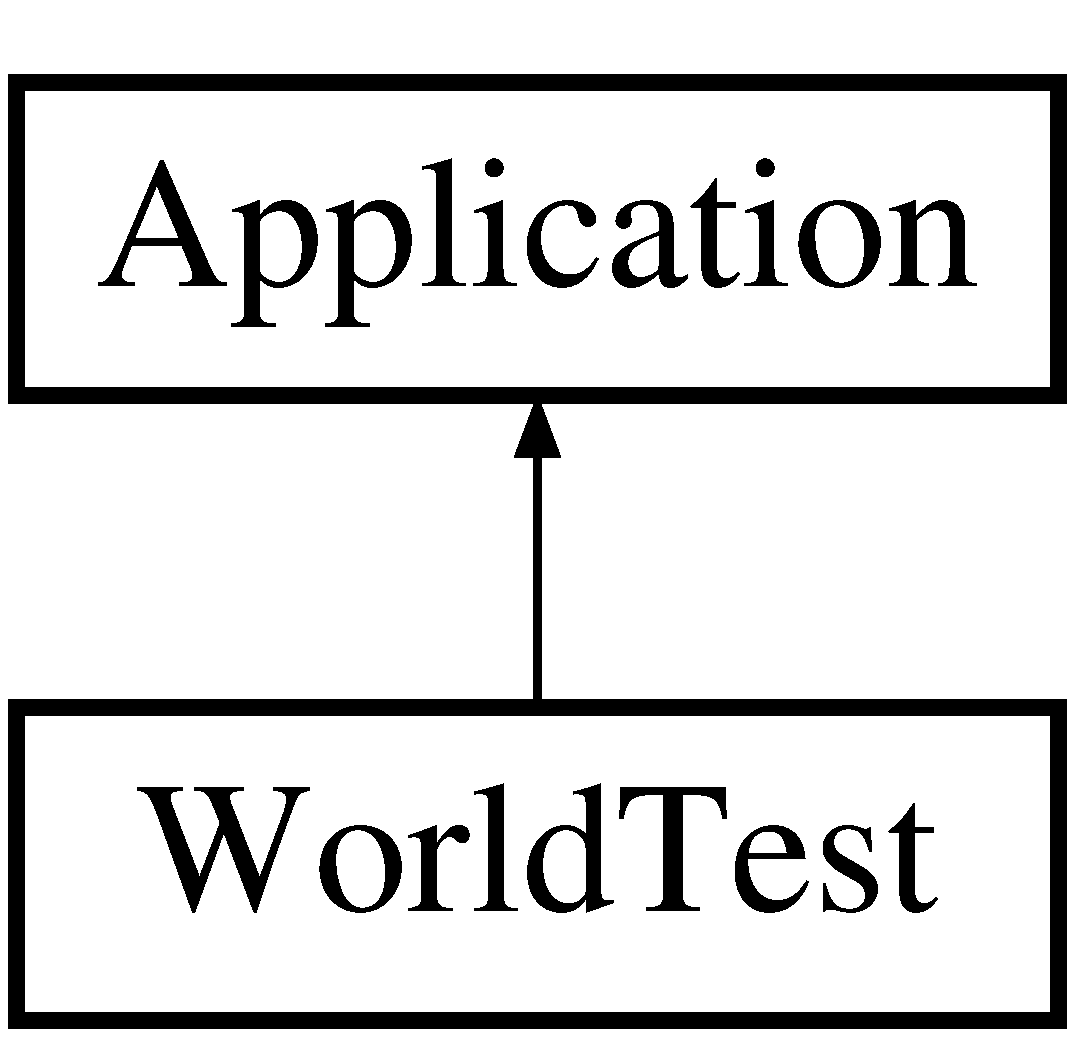
\includegraphics[height=2.000000cm]{class_world_test}
\end{center}
\end{figure}
\subsection*{Public Member Functions}
\begin{DoxyCompactItemize}
\item 
virtual void \hyperlink{class_world_test_aef2eb702d4f558c90308f8cfc0abb128}{on\-Event} (sf\-::\-Event event, sf\-::\-Render\-Window \&window) overridefinal
\begin{DoxyCompactList}\small\item\em Subclass can override this method to handle events. \end{DoxyCompactList}\item 
virtual void \hyperlink{class_world_test_a2dbf8fe3f7de226b01cd284d8b44816e}{on\-Draw} (sf\-::\-Render\-Target \&target) overridefinal
\begin{DoxyCompactList}\small\item\em Subclass can override this method to draw their data in the simulation view. \end{DoxyCompactList}\end{DoxyCompactItemize}
\subsection*{Private Attributes}
\begin{DoxyCompactItemize}
\item 
\hyperlink{class_world}{World} \hyperlink{class_world_test_aa61038592e5857eb9b71d458ccb62cc2}{m\-World}
\end{DoxyCompactItemize}


\subsection{Detailed Description}
Test world procedural generation.

Initially the world is {\itshape not} initialised. One can load a world from a file, or reset the world to initialised the seed and then manually generate the world, or generate a new world using the application settings.

Actions\-:


\begin{DoxyItemize}
\item I\-: load world from file
\item O\-: save world to file
\item R\-: reset world -- initialise seeds
\item Shift+\-R\-: reset world -- generate a new world using cfg settings
\item Space\-: after seeds are initialised, apply one step of the p.\-g. algorithm
\item Shift+\-Space\-: idem, but apply 100 steps
\item S\-: after seeds are initialised, apply one smoothing pass
\item Shift+\-S\-: idem, but apply 10 smoothing passes 
\end{DoxyItemize}

\subsection{Member Function Documentation}
\hypertarget{class_world_test_a2dbf8fe3f7de226b01cd284d8b44816e}{\index{World\-Test@{World\-Test}!on\-Draw@{on\-Draw}}
\index{on\-Draw@{on\-Draw}!WorldTest@{World\-Test}}
\subsubsection[{on\-Draw}]{\setlength{\rightskip}{0pt plus 5cm}void World\-Test\-::on\-Draw (
\begin{DoxyParamCaption}
\item[{sf\-::\-Render\-Target \&}]{target}
\end{DoxyParamCaption}
)\hspace{0.3cm}{\ttfamily [final]}, {\ttfamily [override]}, {\ttfamily [virtual]}}}\label{class_world_test_a2dbf8fe3f7de226b01cd284d8b44816e}


Subclass can override this method to draw their data in the simulation view. 

The default implementation does nothing. However, the env is always displayed first.


\begin{DoxyParams}{Parameters}
{\em target} & a render target \\
\hline
\end{DoxyParams}


Reimplemented from \hyperlink{class_application_ac35bfbd486eb47fdd2b5d731962c6724}{Application}.

\hypertarget{class_world_test_aef2eb702d4f558c90308f8cfc0abb128}{\index{World\-Test@{World\-Test}!on\-Event@{on\-Event}}
\index{on\-Event@{on\-Event}!WorldTest@{World\-Test}}
\subsubsection[{on\-Event}]{\setlength{\rightskip}{0pt plus 5cm}void World\-Test\-::on\-Event (
\begin{DoxyParamCaption}
\item[{sf\-::\-Event}]{event, }
\item[{sf\-::\-Render\-Window \&}]{window}
\end{DoxyParamCaption}
)\hspace{0.3cm}{\ttfamily [final]}, {\ttfamily [override]}, {\ttfamily [virtual]}}}\label{class_world_test_aef2eb702d4f558c90308f8cfc0abb128}


Subclass can override this method to handle events. 

The default implementation does nothing.


\begin{DoxyParams}{Parameters}
{\em event} & an event \\
\hline
{\em window} & the window that emitted the event \\
\hline
\end{DoxyParams}


Reimplemented from \hyperlink{class_application_ae6ea28bafe249f7005aa143f36651342}{Application}.



\subsection{Member Data Documentation}
\hypertarget{class_world_test_aa61038592e5857eb9b71d458ccb62cc2}{\index{World\-Test@{World\-Test}!m\-World@{m\-World}}
\index{m\-World@{m\-World}!WorldTest@{World\-Test}}
\subsubsection[{m\-World}]{\setlength{\rightskip}{0pt plus 5cm}{\bf World} World\-Test\-::m\-World\hspace{0.3cm}{\ttfamily [private]}}}\label{class_world_test_aa61038592e5857eb9b71d458ccb62cc2}


The documentation for this class was generated from the following file\-:\begin{DoxyCompactItemize}
\item 
/home/jbesson/myfiles/cpp/svprog/partie1/src/\-Tests/\-Graphical\-Tests/\hyperlink{_world_test_8cpp}{World\-Test.\-cpp}\end{DoxyCompactItemize}

\chapter{File Documentation}
\hypertarget{_application_8cpp}{\section{/home/jbesson/myfiles/cpp/svprog/partie1/src/\-Application.cpp File Reference}
\label{_application_8cpp}\index{/home/jbesson/myfiles/cpp/svprog/partie1/src/\-Application.\-cpp@{/home/jbesson/myfiles/cpp/svprog/partie1/src/\-Application.\-cpp}}
}
{\ttfamily \#include $<$Application.\-hpp$>$}\\*
{\ttfamily \#include $<$Config.\-hpp$>$}\\*
{\ttfamily \#include $<$J\-S\-O\-N/\-J\-S\-O\-N\-Serialiser.\-hpp$>$}\\*
{\ttfamily \#include $<$Utility/\-Constants.\-hpp$>$}\\*
{\ttfamily \#include $<$algorithm$>$}\\*
{\ttfamily \#include $<$cassert$>$}\\*
\subsection*{Functions}
\begin{DoxyCompactItemize}
\item 
\hyperlink{class_application}{Application} \& \hyperlink{_application_8cpp_a8f44ecc5bce6861fe0e1e7ba6d579d67}{get\-App} ()
\begin{DoxyCompactList}\small\item\em Get the current instance of \hyperlink{class_application}{Application}. \end{DoxyCompactList}\item 
Env \& \hyperlink{_application_8cpp_a297522bb6f68b7f688c91a569f805ad5}{get\-App\-Env} ()
\begin{DoxyCompactList}\small\item\em Get the environment (the env) of the current application. \end{DoxyCompactList}\item 
\hyperlink{classj_1_1_value}{j\-::\-Value} \& \hyperlink{_application_8cpp_ac7728cb634dcf024e679116d7b6b1c85}{get\-App\-Config} ()
\begin{DoxyCompactList}\small\item\em Get the bee tracker helper for the current application. \end{DoxyCompactList}\item 
sf\-::\-Font const \& \hyperlink{_application_8cpp_aad5996611619196f44218c9a9b66a3ed}{get\-App\-Font} ()
\begin{DoxyCompactList}\small\item\em Get the app's font. \end{DoxyCompactList}\item 
sf\-::\-Texture \& \hyperlink{_application_8cpp_aa4a7cff7b1c9246a309a312fc6e4c165}{get\-App\-Texture} (std\-::string const \&name)
\begin{DoxyCompactList}\small\item\em Get a texture. \end{DoxyCompactList}\item 
bool \hyperlink{_application_8cpp_a6d9dec2d69ed42ef4d8cb1c823134047}{is\-Debug\-On} ()
\begin{DoxyCompactList}\small\item\em Determine if debug mode is active or not. \end{DoxyCompactList}\end{DoxyCompactItemize}


\subsection{Function Documentation}
\hypertarget{_application_8cpp_a8f44ecc5bce6861fe0e1e7ba6d579d67}{\index{Application.\-cpp@{Application.\-cpp}!get\-App@{get\-App}}
\index{get\-App@{get\-App}!Application.cpp@{Application.\-cpp}}
\subsubsection[{get\-App}]{\setlength{\rightskip}{0pt plus 5cm}{\bf Application}\& get\-App (
\begin{DoxyParamCaption}
{}
\end{DoxyParamCaption}
)}}\label{_application_8cpp_a8f44ecc5bce6861fe0e1e7ba6d579d67}


Get the current instance of \hyperlink{class_application}{Application}. 

\begin{DoxyReturn}{Returns}
a reference to the current instance of \hyperlink{class_application}{Application} 
\end{DoxyReturn}
\hypertarget{_application_8cpp_ac7728cb634dcf024e679116d7b6b1c85}{\index{Application.\-cpp@{Application.\-cpp}!get\-App\-Config@{get\-App\-Config}}
\index{get\-App\-Config@{get\-App\-Config}!Application.cpp@{Application.\-cpp}}
\subsubsection[{get\-App\-Config}]{\setlength{\rightskip}{0pt plus 5cm}{\bf j\-::\-Value}\& get\-App\-Config (
\begin{DoxyParamCaption}
{}
\end{DoxyParamCaption}
)}}\label{_application_8cpp_ac7728cb634dcf024e679116d7b6b1c85}


Get the bee tracker helper for the current application. 

\begin{DoxyReturn}{Returns}
the app's bee tracker
\end{DoxyReturn}
Get the config of the current application

Shorthand for \hyperlink{_application_8hpp_a8f44ecc5bce6861fe0e1e7ba6d579d67}{get\-App()}.get\-Config()

\begin{DoxyReturn}{Returns}
the app's config 
\end{DoxyReturn}
\hypertarget{_application_8cpp_a297522bb6f68b7f688c91a569f805ad5}{\index{Application.\-cpp@{Application.\-cpp}!get\-App\-Env@{get\-App\-Env}}
\index{get\-App\-Env@{get\-App\-Env}!Application.cpp@{Application.\-cpp}}
\subsubsection[{get\-App\-Env}]{\setlength{\rightskip}{0pt plus 5cm}Env\& get\-App\-Env (
\begin{DoxyParamCaption}
{}
\end{DoxyParamCaption}
)}}\label{_application_8cpp_a297522bb6f68b7f688c91a569f805ad5}


Get the environment (the env) of the current application. 

Shorthand for \hyperlink{_application_8hpp_a8f44ecc5bce6861fe0e1e7ba6d579d67}{get\-App()}.get\-Env()

\begin{DoxySeeAlso}{See Also}
\hyperlink{class_application_a66c2e8b7340252006680158876db46e1}{Application\-::get\-Env()} comment about encapsulation
\end{DoxySeeAlso}
\begin{DoxyReturn}{Returns}
the app's env. 
\end{DoxyReturn}
\hypertarget{_application_8cpp_aad5996611619196f44218c9a9b66a3ed}{\index{Application.\-cpp@{Application.\-cpp}!get\-App\-Font@{get\-App\-Font}}
\index{get\-App\-Font@{get\-App\-Font}!Application.cpp@{Application.\-cpp}}
\subsubsection[{get\-App\-Font}]{\setlength{\rightskip}{0pt plus 5cm}sf\-::\-Font const\& get\-App\-Font (
\begin{DoxyParamCaption}
{}
\end{DoxyParamCaption}
)}}\label{_application_8cpp_aad5996611619196f44218c9a9b66a3ed}


Get the app's font. 

Shorthand for \hyperlink{_application_8hpp_a8f44ecc5bce6861fe0e1e7ba6d579d67}{get\-App()}.get\-Font()

\begin{DoxyReturn}{Returns}
a font 
\end{DoxyReturn}
\hypertarget{_application_8cpp_aa4a7cff7b1c9246a309a312fc6e4c165}{\index{Application.\-cpp@{Application.\-cpp}!get\-App\-Texture@{get\-App\-Texture}}
\index{get\-App\-Texture@{get\-App\-Texture}!Application.cpp@{Application.\-cpp}}
\subsubsection[{get\-App\-Texture}]{\setlength{\rightskip}{0pt plus 5cm}sf\-::\-Texture\& get\-App\-Texture (
\begin{DoxyParamCaption}
\item[{std\-::string const \&}]{name}
\end{DoxyParamCaption}
)}}\label{_application_8cpp_aa4a7cff7b1c9246a309a312fc6e4c165}


Get a texture. 

Shorthand for \hyperlink{_application_8hpp_a8f44ecc5bce6861fe0e1e7ba6d579d67}{get\-App()}.get\-Texture(name)


\begin{DoxyParams}{Parameters}
{\em name} & name of the texture \\
\hline
\end{DoxyParams}
\begin{DoxyReturn}{Returns}
a reference to the texture
\end{DoxyReturn}
\begin{DoxySeeAlso}{See Also}
\hyperlink{class_application_a18f35a0326625f9818003dc7353d4208}{Application\-::get\-Texture} 
\end{DoxySeeAlso}
\hypertarget{_application_8cpp_a6d9dec2d69ed42ef4d8cb1c823134047}{\index{Application.\-cpp@{Application.\-cpp}!is\-Debug\-On@{is\-Debug\-On}}
\index{is\-Debug\-On@{is\-Debug\-On}!Application.cpp@{Application.\-cpp}}
\subsubsection[{is\-Debug\-On}]{\setlength{\rightskip}{0pt plus 5cm}bool is\-Debug\-On (
\begin{DoxyParamCaption}
{}
\end{DoxyParamCaption}
)}}\label{_application_8cpp_a6d9dec2d69ed42ef4d8cb1c823134047}


Determine if debug mode is active or not. 

Shorthand for \hyperlink{_application_8hpp_ac7728cb634dcf024e679116d7b6b1c85}{get\-App\-Config()}.get\-Bool(\-D\-E\-B\-U\-G\-\_\-\-M\-O\-D\-E)

\begin{DoxyReturn}{Returns}
true if cfg specify D\-E\-B\-U\-G=T\-R\-U\-E 
\end{DoxyReturn}

\hypertarget{_application_8hpp}{\section{/home/jbesson/myfiles/cpp/svprog/partie1/src/\-Application.hpp File Reference}
\label{_application_8hpp}\index{/home/jbesson/myfiles/cpp/svprog/partie1/src/\-Application.\-hpp@{/home/jbesson/myfiles/cpp/svprog/partie1/src/\-Application.\-hpp}}
}
{\ttfamily \#include $<$J\-S\-O\-N/\-J\-S\-O\-N.\-hpp$>$}\\*
{\ttfamily \#include $<$Utility/\-Vec2d.\-hpp$>$}\\*
{\ttfamily \#include $<$S\-F\-M\-L/\-Graphics.\-hpp$>$}\\*
{\ttfamily \#include $<$iostream$>$}\\*
{\ttfamily \#include $<$list$>$}\\*
{\ttfamily \#include $<$map$>$}\\*
{\ttfamily \#include $<$stdexcept$>$}\\*
{\ttfamily \#include $<$string$>$}\\*
\subsection*{Classes}
\begin{DoxyCompactItemize}
\item 
class \hyperlink{class_application}{Application}
\begin{DoxyCompactList}\small\item\em Abstract class managing the core of the program. \end{DoxyCompactList}\end{DoxyCompactItemize}
\subsection*{Macros}
\begin{DoxyCompactItemize}
\item 
\#define \hyperlink{_application_8hpp_a53f1a3ed7b211528d3721f9bd53cc1e2}{I\-M\-P\-L\-E\-M\-E\-N\-T\-\_\-\-M\-A\-I\-N}(A\-P\-P\-L\-I\-C\-A\-T\-I\-O\-N\-\_\-\-C\-L\-A\-S\-S)
\begin{DoxyCompactList}\small\item\em Define a few macros. \end{DoxyCompactList}\item 
\#define \hyperlink{_application_8hpp_aea9b5e95c652bca200f8361755856589}{I\-N\-I\-T\-\_\-\-D\-E\-F\-A\-U\-L\-T\-\_\-\-A\-P\-P}(argc, argv)~\hyperlink{class_application}{Application} app((argc), (argv));
\end{DoxyCompactItemize}
\subsection*{Functions}
\begin{DoxyCompactItemize}
\item 
\hyperlink{class_application}{Application} \& \hyperlink{_application_8hpp_a8f44ecc5bce6861fe0e1e7ba6d579d67}{get\-App} ()
\begin{DoxyCompactList}\small\item\em Get the current instance of \hyperlink{class_application}{Application}. \end{DoxyCompactList}\item 
Env \& \hyperlink{_application_8hpp_a297522bb6f68b7f688c91a569f805ad5}{get\-App\-Env} ()
\begin{DoxyCompactList}\small\item\em Get the environment (the env) of the current application. \end{DoxyCompactList}\item 
\hyperlink{classj_1_1_value}{j\-::\-Value} \& \hyperlink{_application_8hpp_ac7728cb634dcf024e679116d7b6b1c85}{get\-App\-Config} ()
\begin{DoxyCompactList}\small\item\em Get the bee tracker helper for the current application. \end{DoxyCompactList}\item 
sf\-::\-Font const \& \hyperlink{_application_8hpp_aad5996611619196f44218c9a9b66a3ed}{get\-App\-Font} ()
\begin{DoxyCompactList}\small\item\em Get the app's font. \end{DoxyCompactList}\item 
sf\-::\-Texture \& \hyperlink{_application_8hpp_aa4a7cff7b1c9246a309a312fc6e4c165}{get\-App\-Texture} (std\-::string const \&name)
\begin{DoxyCompactList}\small\item\em Get a texture. \end{DoxyCompactList}\item 
bool \hyperlink{_application_8hpp_a6d9dec2d69ed42ef4d8cb1c823134047}{is\-Debug\-On} ()
\begin{DoxyCompactList}\small\item\em Determine if debug mode is active or not. \end{DoxyCompactList}\end{DoxyCompactItemize}


\subsection{Macro Definition Documentation}
\hypertarget{_application_8hpp_a53f1a3ed7b211528d3721f9bd53cc1e2}{\index{Application.\-hpp@{Application.\-hpp}!I\-M\-P\-L\-E\-M\-E\-N\-T\-\_\-\-M\-A\-I\-N@{I\-M\-P\-L\-E\-M\-E\-N\-T\-\_\-\-M\-A\-I\-N}}
\index{I\-M\-P\-L\-E\-M\-E\-N\-T\-\_\-\-M\-A\-I\-N@{I\-M\-P\-L\-E\-M\-E\-N\-T\-\_\-\-M\-A\-I\-N}!Application.hpp@{Application.\-hpp}}
\subsubsection[{I\-M\-P\-L\-E\-M\-E\-N\-T\-\_\-\-M\-A\-I\-N}]{\setlength{\rightskip}{0pt plus 5cm}\#define I\-M\-P\-L\-E\-M\-E\-N\-T\-\_\-\-M\-A\-I\-N(
\begin{DoxyParamCaption}
\item[{}]{A\-P\-P\-L\-I\-C\-A\-T\-I\-O\-N\-\_\-\-C\-L\-A\-S\-S}
\end{DoxyParamCaption}
)}}\label{_application_8hpp_a53f1a3ed7b211528d3721f9bd53cc1e2}
{\bfseries Value\-:}
\begin{DoxyCode}
\textcolor{keywordtype}{int} \hyperlink{_catch_tests_8cpp_a790aa8b99fa3d90918361b8936af0b14}{main}(\textcolor{keywordtype}{int} argc, \textcolor{keywordtype}{char} \textcolor{keyword}{const}** argv)                   \(\backslash\)
    try \{                                                   \(\backslash\)
        APPLICATION\_CLASS app(argc, argv);                  \(\backslash\)
        app.run();                                          \(\backslash\)
        return 0;                                           \(\backslash\)
    \} \textcolor{keywordflow}{catch} (std::exception \textcolor{keyword}{const}& e) \{                     \(\backslash\)
        std::cerr << \textcolor{stringliteral}{"FATAL ERROR: "} << e.what() << \textcolor{stringliteral}{"\(\backslash\)n"};   \(\backslash\)
        return 1;                                           \(\backslash\)
    \}
\end{DoxyCode}


Define a few macros. 

Implement the \hyperlink{_catch_tests_8cpp_a790aa8b99fa3d90918361b8936af0b14}{main()} function with a given subclass of \hyperlink{class_application}{Application}


\begin{DoxyParams}{Parameters}
{\em A\-P\-P\-L\-I\-C\-A\-T\-I\-O\-N\-\_\-\-C\-L\-A\-S\-S} & a class name (it must be a subclass of \hyperlink{class_application}{Application}) \\
\hline
\end{DoxyParams}
\hypertarget{_application_8hpp_aea9b5e95c652bca200f8361755856589}{\index{Application.\-hpp@{Application.\-hpp}!I\-N\-I\-T\-\_\-\-D\-E\-F\-A\-U\-L\-T\-\_\-\-A\-P\-P@{I\-N\-I\-T\-\_\-\-D\-E\-F\-A\-U\-L\-T\-\_\-\-A\-P\-P}}
\index{I\-N\-I\-T\-\_\-\-D\-E\-F\-A\-U\-L\-T\-\_\-\-A\-P\-P@{I\-N\-I\-T\-\_\-\-D\-E\-F\-A\-U\-L\-T\-\_\-\-A\-P\-P}!Application.hpp@{Application.\-hpp}}
\subsubsection[{I\-N\-I\-T\-\_\-\-D\-E\-F\-A\-U\-L\-T\-\_\-\-A\-P\-P}]{\setlength{\rightskip}{0pt plus 5cm}\#define I\-N\-I\-T\-\_\-\-D\-E\-F\-A\-U\-L\-T\-\_\-\-A\-P\-P(
\begin{DoxyParamCaption}
\item[{}]{argc, }
\item[{}]{argv}
\end{DoxyParamCaption}
)~{\bf Application} app((argc), (argv));}}\label{_application_8hpp_aea9b5e95c652bca200f8361755856589}


\subsection{Function Documentation}
\hypertarget{_application_8hpp_a8f44ecc5bce6861fe0e1e7ba6d579d67}{\index{Application.\-hpp@{Application.\-hpp}!get\-App@{get\-App}}
\index{get\-App@{get\-App}!Application.hpp@{Application.\-hpp}}
\subsubsection[{get\-App}]{\setlength{\rightskip}{0pt plus 5cm}{\bf Application}\& get\-App (
\begin{DoxyParamCaption}
{}
\end{DoxyParamCaption}
)}}\label{_application_8hpp_a8f44ecc5bce6861fe0e1e7ba6d579d67}


Get the current instance of \hyperlink{class_application}{Application}. 

\begin{DoxyReturn}{Returns}
a reference to the current instance of \hyperlink{class_application}{Application} 
\end{DoxyReturn}
\hypertarget{_application_8hpp_ac7728cb634dcf024e679116d7b6b1c85}{\index{Application.\-hpp@{Application.\-hpp}!get\-App\-Config@{get\-App\-Config}}
\index{get\-App\-Config@{get\-App\-Config}!Application.hpp@{Application.\-hpp}}
\subsubsection[{get\-App\-Config}]{\setlength{\rightskip}{0pt plus 5cm}{\bf j\-::\-Value}\& get\-App\-Config (
\begin{DoxyParamCaption}
{}
\end{DoxyParamCaption}
)}}\label{_application_8hpp_ac7728cb634dcf024e679116d7b6b1c85}


Get the bee tracker helper for the current application. 

\begin{DoxyReturn}{Returns}
the app's bee tracker
\end{DoxyReturn}
Get the config of the current application

Shorthand for \hyperlink{_application_8hpp_a8f44ecc5bce6861fe0e1e7ba6d579d67}{get\-App()}.get\-Config()

\begin{DoxyReturn}{Returns}
the app's config 
\end{DoxyReturn}
\hypertarget{_application_8hpp_a297522bb6f68b7f688c91a569f805ad5}{\index{Application.\-hpp@{Application.\-hpp}!get\-App\-Env@{get\-App\-Env}}
\index{get\-App\-Env@{get\-App\-Env}!Application.hpp@{Application.\-hpp}}
\subsubsection[{get\-App\-Env}]{\setlength{\rightskip}{0pt plus 5cm}Env\& get\-App\-Env (
\begin{DoxyParamCaption}
{}
\end{DoxyParamCaption}
)}}\label{_application_8hpp_a297522bb6f68b7f688c91a569f805ad5}


Get the environment (the env) of the current application. 

Shorthand for \hyperlink{_application_8hpp_a8f44ecc5bce6861fe0e1e7ba6d579d67}{get\-App()}.get\-Env()

\begin{DoxySeeAlso}{See Also}
\hyperlink{class_application_a66c2e8b7340252006680158876db46e1}{Application\-::get\-Env()} comment about encapsulation
\end{DoxySeeAlso}
\begin{DoxyReturn}{Returns}
the app's env. 
\end{DoxyReturn}
\hypertarget{_application_8hpp_aad5996611619196f44218c9a9b66a3ed}{\index{Application.\-hpp@{Application.\-hpp}!get\-App\-Font@{get\-App\-Font}}
\index{get\-App\-Font@{get\-App\-Font}!Application.hpp@{Application.\-hpp}}
\subsubsection[{get\-App\-Font}]{\setlength{\rightskip}{0pt plus 5cm}sf\-::\-Font const\& get\-App\-Font (
\begin{DoxyParamCaption}
{}
\end{DoxyParamCaption}
)}}\label{_application_8hpp_aad5996611619196f44218c9a9b66a3ed}


Get the app's font. 

Shorthand for \hyperlink{_application_8hpp_a8f44ecc5bce6861fe0e1e7ba6d579d67}{get\-App()}.get\-Font()

\begin{DoxyReturn}{Returns}
a font 
\end{DoxyReturn}
\hypertarget{_application_8hpp_aa4a7cff7b1c9246a309a312fc6e4c165}{\index{Application.\-hpp@{Application.\-hpp}!get\-App\-Texture@{get\-App\-Texture}}
\index{get\-App\-Texture@{get\-App\-Texture}!Application.hpp@{Application.\-hpp}}
\subsubsection[{get\-App\-Texture}]{\setlength{\rightskip}{0pt plus 5cm}sf\-::\-Texture\& get\-App\-Texture (
\begin{DoxyParamCaption}
\item[{std\-::string const \&}]{name}
\end{DoxyParamCaption}
)}}\label{_application_8hpp_aa4a7cff7b1c9246a309a312fc6e4c165}


Get a texture. 

Shorthand for \hyperlink{_application_8hpp_a8f44ecc5bce6861fe0e1e7ba6d579d67}{get\-App()}.get\-Texture(name)


\begin{DoxyParams}{Parameters}
{\em name} & name of the texture \\
\hline
\end{DoxyParams}
\begin{DoxyReturn}{Returns}
a reference to the texture
\end{DoxyReturn}
\begin{DoxySeeAlso}{See Also}
\hyperlink{class_application_a18f35a0326625f9818003dc7353d4208}{Application\-::get\-Texture} 
\end{DoxySeeAlso}
\hypertarget{_application_8hpp_a6d9dec2d69ed42ef4d8cb1c823134047}{\index{Application.\-hpp@{Application.\-hpp}!is\-Debug\-On@{is\-Debug\-On}}
\index{is\-Debug\-On@{is\-Debug\-On}!Application.hpp@{Application.\-hpp}}
\subsubsection[{is\-Debug\-On}]{\setlength{\rightskip}{0pt plus 5cm}bool is\-Debug\-On (
\begin{DoxyParamCaption}
{}
\end{DoxyParamCaption}
)}}\label{_application_8hpp_a6d9dec2d69ed42ef4d8cb1c823134047}


Determine if debug mode is active or not. 

Shorthand for \hyperlink{_application_8hpp_ac7728cb634dcf024e679116d7b6b1c85}{get\-App\-Config()}.get\-Bool(\-D\-E\-B\-U\-G\-\_\-\-M\-O\-D\-E)

\begin{DoxyReturn}{Returns}
true if cfg specify D\-E\-B\-U\-G=T\-R\-U\-E 
\end{DoxyReturn}

\hypertarget{_config_8hpp}{\section{/home/jbesson/myfiles/cpp/svprog/partie1/src/\-Config.hpp File Reference}
\label{_config_8hpp}\index{/home/jbesson/myfiles/cpp/svprog/partie1/src/\-Config.\-hpp@{/home/jbesson/myfiles/cpp/svprog/partie1/src/\-Config.\-hpp}}
}
{\ttfamily \#include $<$string$>$}\\*
\subsection*{Variables}
\begin{DoxyCompactItemize}
\item 
std\-::string const \hyperlink{_config_8hpp_a84a8277d12bf2ad6d23fe183610fe4a6}{R\-E\-S\-\_\-\-L\-O\-C\-A\-T\-I\-O\-N} = \char`\"{}../res/\char`\"{}
\item 
std\-::string const \hyperlink{_config_8hpp_a17c02f9505bae36ce2d5119331f69224}{D\-E\-F\-A\-U\-L\-T\-\_\-\-C\-F\-G} = \char`\"{}app.\-json\char`\"{}
\item 
std\-::string const \hyperlink{_config_8hpp_af76dceeab24b236f9f2cdab538cf002a}{F\-O\-N\-T\-\_\-\-L\-O\-C\-A\-T\-I\-O\-N} = \hyperlink{_config_8hpp_a84a8277d12bf2ad6d23fe183610fe4a6}{R\-E\-S\-\_\-\-L\-O\-C\-A\-T\-I\-O\-N} + \char`\"{}sansation.\-ttf\char`\"{}
\end{DoxyCompactItemize}


\subsection{Variable Documentation}
\hypertarget{_config_8hpp_a17c02f9505bae36ce2d5119331f69224}{\index{Config.\-hpp@{Config.\-hpp}!D\-E\-F\-A\-U\-L\-T\-\_\-\-C\-F\-G@{D\-E\-F\-A\-U\-L\-T\-\_\-\-C\-F\-G}}
\index{D\-E\-F\-A\-U\-L\-T\-\_\-\-C\-F\-G@{D\-E\-F\-A\-U\-L\-T\-\_\-\-C\-F\-G}!Config.hpp@{Config.\-hpp}}
\subsubsection[{D\-E\-F\-A\-U\-L\-T\-\_\-\-C\-F\-G}]{\setlength{\rightskip}{0pt plus 5cm}std\-::string const D\-E\-F\-A\-U\-L\-T\-\_\-\-C\-F\-G = \char`\"{}app.\-json\char`\"{}}}\label{_config_8hpp_a17c02f9505bae36ce2d5119331f69224}
\hypertarget{_config_8hpp_af76dceeab24b236f9f2cdab538cf002a}{\index{Config.\-hpp@{Config.\-hpp}!F\-O\-N\-T\-\_\-\-L\-O\-C\-A\-T\-I\-O\-N@{F\-O\-N\-T\-\_\-\-L\-O\-C\-A\-T\-I\-O\-N}}
\index{F\-O\-N\-T\-\_\-\-L\-O\-C\-A\-T\-I\-O\-N@{F\-O\-N\-T\-\_\-\-L\-O\-C\-A\-T\-I\-O\-N}!Config.hpp@{Config.\-hpp}}
\subsubsection[{F\-O\-N\-T\-\_\-\-L\-O\-C\-A\-T\-I\-O\-N}]{\setlength{\rightskip}{0pt plus 5cm}std\-::string const F\-O\-N\-T\-\_\-\-L\-O\-C\-A\-T\-I\-O\-N = {\bf R\-E\-S\-\_\-\-L\-O\-C\-A\-T\-I\-O\-N} + \char`\"{}sansation.\-ttf\char`\"{}}}\label{_config_8hpp_af76dceeab24b236f9f2cdab538cf002a}
\hypertarget{_config_8hpp_a84a8277d12bf2ad6d23fe183610fe4a6}{\index{Config.\-hpp@{Config.\-hpp}!R\-E\-S\-\_\-\-L\-O\-C\-A\-T\-I\-O\-N@{R\-E\-S\-\_\-\-L\-O\-C\-A\-T\-I\-O\-N}}
\index{R\-E\-S\-\_\-\-L\-O\-C\-A\-T\-I\-O\-N@{R\-E\-S\-\_\-\-L\-O\-C\-A\-T\-I\-O\-N}!Config.hpp@{Config.\-hpp}}
\subsubsection[{R\-E\-S\-\_\-\-L\-O\-C\-A\-T\-I\-O\-N}]{\setlength{\rightskip}{0pt plus 5cm}std\-::string const R\-E\-S\-\_\-\-L\-O\-C\-A\-T\-I\-O\-N = \char`\"{}../res/\char`\"{}}}\label{_config_8hpp_a84a8277d12bf2ad6d23fe183610fe4a6}

\hypertarget{_collider_8cpp}{\section{/home/jbesson/myfiles/cpp/svprog/partie1/src/\-Env/\-Collider.cpp File Reference}
\label{_collider_8cpp}\index{/home/jbesson/myfiles/cpp/svprog/partie1/src/\-Env/\-Collider.\-cpp@{/home/jbesson/myfiles/cpp/svprog/partie1/src/\-Env/\-Collider.\-cpp}}
}
{\ttfamily \#include \char`\"{}Collider.\-hpp\char`\"{}}\\*
{\ttfamily \#include $<$iostream$>$}\\*
{\ttfamily \#include \char`\"{}../\-Utility/\-Vec2d.\-hpp\char`\"{}}\\*
{\ttfamily \#include $<$Application.\-hpp$>$}\\*
{\ttfamily \#include $<$cassert$>$}\\*
{\ttfamily \#include $<$vector$>$}\\*
\subsection*{Functions}
\begin{DoxyCompactItemize}
\item 
std\-::ostream \& \hyperlink{_collider_8cpp_a3326283ecfaefb7c97bceb1a72383227}{operator$<$$<$} (std\-::ostream \&oss, const \hyperlink{class_collider}{Collider} \&collider)
\end{DoxyCompactItemize}


\subsection{Function Documentation}
\hypertarget{_collider_8cpp_a3326283ecfaefb7c97bceb1a72383227}{\index{Collider.\-cpp@{Collider.\-cpp}!operator$<$$<$@{operator$<$$<$}}
\index{operator$<$$<$@{operator$<$$<$}!Collider.cpp@{Collider.\-cpp}}
\subsubsection[{operator$<$$<$}]{\setlength{\rightskip}{0pt plus 5cm}std\-::ostream\& operator$<$$<$ (
\begin{DoxyParamCaption}
\item[{std\-::ostream \&}]{oss, }
\item[{const {\bf Collider} \&}]{collider}
\end{DoxyParamCaption}
)}}\label{_collider_8cpp_a3326283ecfaefb7c97bceb1a72383227}
Print the contents of this to a stream. 
\begin{DoxyParams}{Parameters}
{\em oss} & stream to print to. \\
\hline
{\em collider} & \hyperlink{class_collider}{Collider} to print from. \\
\hline
\end{DoxyParams}

\hypertarget{_collider_8hpp}{\section{/home/jbesson/myfiles/cpp/svprog/partie1/src/\-Env/\-Collider.hpp File Reference}
\label{_collider_8hpp}\index{/home/jbesson/myfiles/cpp/svprog/partie1/src/\-Env/\-Collider.\-hpp@{/home/jbesson/myfiles/cpp/svprog/partie1/src/\-Env/\-Collider.\-hpp}}
}
{\ttfamily \#include \char`\"{}../\-Utility/\-Vec2d.\-hpp\char`\"{}}\\*
\subsection*{Classes}
\begin{DoxyCompactItemize}
\item 
class \hyperlink{class_collider}{Collider}
\end{DoxyCompactItemize}
\subsection*{Functions}
\begin{DoxyCompactItemize}
\item 
std\-::ostream \& \hyperlink{_collider_8hpp_a3326283ecfaefb7c97bceb1a72383227}{operator$<$$<$} (std\-::ostream \&oss, const \hyperlink{class_collider}{Collider} \&collider)
\end{DoxyCompactItemize}


\subsection{Function Documentation}
\hypertarget{_collider_8hpp_a3326283ecfaefb7c97bceb1a72383227}{\index{Collider.\-hpp@{Collider.\-hpp}!operator$<$$<$@{operator$<$$<$}}
\index{operator$<$$<$@{operator$<$$<$}!Collider.hpp@{Collider.\-hpp}}
\subsubsection[{operator$<$$<$}]{\setlength{\rightskip}{0pt plus 5cm}std\-::ostream\& operator$<$$<$ (
\begin{DoxyParamCaption}
\item[{std\-::ostream \&}]{oss, }
\item[{const {\bf Collider} \&}]{collider}
\end{DoxyParamCaption}
)}}\label{_collider_8hpp_a3326283ecfaefb7c97bceb1a72383227}
Print the contents of this to a stream. 
\begin{DoxyParams}{Parameters}
{\em oss} & stream to print to. \\
\hline
{\em collider} & \hyperlink{class_collider}{Collider} to print from. \\
\hline
\end{DoxyParams}

\hypertarget{_world_8hpp}{\section{/home/jbesson/myfiles/cpp/svprog/partie1/src/\-Env/\-World.hpp File Reference}
\label{_world_8hpp}\index{/home/jbesson/myfiles/cpp/svprog/partie1/src/\-Env/\-World.\-hpp@{/home/jbesson/myfiles/cpp/svprog/partie1/src/\-Env/\-World.\-hpp}}
}
\subsection*{Classes}
\begin{DoxyCompactItemize}
\item 
class \hyperlink{class_world}{World}
\end{DoxyCompactItemize}
\subsection*{Enumerations}
\begin{DoxyCompactItemize}
\item 
enum \hyperlink{_world_8hpp_a3a66ab4f6059050f3fce0595886ea4c5}{Kind} \-: short \{ \hyperlink{_world_8hpp_a3a66ab4f6059050f3fce0595886ea4c5aaac9a63596f76a62bb9f61a5dd7c0d25}{Kind\-::\-Grass}, 
\hyperlink{_world_8hpp_a3a66ab4f6059050f3fce0595886ea4c5a27634ff8002b12e75d98e07ccd005d18}{Kind\-::\-Water}, 
\hyperlink{_world_8hpp_a3a66ab4f6059050f3fce0595886ea4c5a4cfbb125e9878528bab91d12421134d8}{Kind\-::\-Rock}
 \}
\end{DoxyCompactItemize}


\subsection{Enumeration Type Documentation}
\hypertarget{_world_8hpp_a3a66ab4f6059050f3fce0595886ea4c5}{\index{World.\-hpp@{World.\-hpp}!Kind@{Kind}}
\index{Kind@{Kind}!World.hpp@{World.\-hpp}}
\subsubsection[{Kind}]{\setlength{\rightskip}{0pt plus 5cm}enum {\bf Kind} \-: short\hspace{0.3cm}{\ttfamily [strong]}}}\label{_world_8hpp_a3a66ab4f6059050f3fce0595886ea4c5}
\begin{Desc}
\item[Enumerator]\par
\begin{description}
\index{Grass@{Grass}!World.\-hpp@{World.\-hpp}}\index{World.\-hpp@{World.\-hpp}!Grass@{Grass}}\item[{\em 
\hypertarget{_world_8hpp_a3a66ab4f6059050f3fce0595886ea4c5aaac9a63596f76a62bb9f61a5dd7c0d25}{Grass}\label{_world_8hpp_a3a66ab4f6059050f3fce0595886ea4c5aaac9a63596f76a62bb9f61a5dd7c0d25}
}]\index{Water@{Water}!World.\-hpp@{World.\-hpp}}\index{World.\-hpp@{World.\-hpp}!Water@{Water}}\item[{\em 
\hypertarget{_world_8hpp_a3a66ab4f6059050f3fce0595886ea4c5a27634ff8002b12e75d98e07ccd005d18}{Water}\label{_world_8hpp_a3a66ab4f6059050f3fce0595886ea4c5a27634ff8002b12e75d98e07ccd005d18}
}]\index{Rock@{Rock}!World.\-hpp@{World.\-hpp}}\index{World.\-hpp@{World.\-hpp}!Rock@{Rock}}\item[{\em 
\hypertarget{_world_8hpp_a3a66ab4f6059050f3fce0595886ea4c5a4cfbb125e9878528bab91d12421134d8}{Rock}\label{_world_8hpp_a3a66ab4f6059050f3fce0595886ea4c5a4cfbb125e9878528bab91d12421134d8}
}]\end{description}
\end{Desc}

\hypertarget{_final_application_8cpp}{\section{/home/jbesson/myfiles/cpp/svprog/partie1/src/\-Final\-Application.cpp File Reference}
\label{_final_application_8cpp}\index{/home/jbesson/myfiles/cpp/svprog/partie1/src/\-Final\-Application.\-cpp@{/home/jbesson/myfiles/cpp/svprog/partie1/src/\-Final\-Application.\-cpp}}
}
{\ttfamily \#include $<$Config.\-hpp$>$}\\*
{\ttfamily \#include $<$Final\-Application.\-hpp$>$}\\*
{\ttfamily \#include $<$cassert$>$}\\*
\subsection*{Functions}
\begin{DoxyCompactItemize}
\item 
\hyperlink{_final_application_8cpp_ab9fb74ed041b1bdbf7109108ff1caa8d}{I\-M\-P\-L\-E\-M\-E\-N\-T\-\_\-\-M\-A\-I\-N} (\hyperlink{class_final_application}{Final\-Application})
\end{DoxyCompactItemize}


\subsection{Function Documentation}
\hypertarget{_final_application_8cpp_ab9fb74ed041b1bdbf7109108ff1caa8d}{\index{Final\-Application.\-cpp@{Final\-Application.\-cpp}!I\-M\-P\-L\-E\-M\-E\-N\-T\-\_\-\-M\-A\-I\-N@{I\-M\-P\-L\-E\-M\-E\-N\-T\-\_\-\-M\-A\-I\-N}}
\index{I\-M\-P\-L\-E\-M\-E\-N\-T\-\_\-\-M\-A\-I\-N@{I\-M\-P\-L\-E\-M\-E\-N\-T\-\_\-\-M\-A\-I\-N}!FinalApplication.cpp@{Final\-Application.\-cpp}}
\subsubsection[{I\-M\-P\-L\-E\-M\-E\-N\-T\-\_\-\-M\-A\-I\-N}]{\setlength{\rightskip}{0pt plus 5cm}I\-M\-P\-L\-E\-M\-E\-N\-T\-\_\-\-M\-A\-I\-N (
\begin{DoxyParamCaption}
\item[{{\bf Final\-Application}}]{}
\end{DoxyParamCaption}
)}}\label{_final_application_8cpp_ab9fb74ed041b1bdbf7109108ff1caa8d}

\hypertarget{_final_application_8hpp}{\section{/home/jbesson/myfiles/cpp/svprog/partie1/src/\-Final\-Application.hpp File Reference}
\label{_final_application_8hpp}\index{/home/jbesson/myfiles/cpp/svprog/partie1/src/\-Final\-Application.\-hpp@{/home/jbesson/myfiles/cpp/svprog/partie1/src/\-Final\-Application.\-hpp}}
}
{\ttfamily \#include $<$Application.\-hpp$>$}\\*
\subsection*{Classes}
\begin{DoxyCompactItemize}
\item 
class \hyperlink{class_final_application}{Final\-Application}
\end{DoxyCompactItemize}

\hypertarget{_drawable_8hpp}{\section{/home/jbesson/myfiles/cpp/svprog/partie1/src/\-Interface/\-Drawable.hpp File Reference}
\label{_drawable_8hpp}\index{/home/jbesson/myfiles/cpp/svprog/partie1/src/\-Interface/\-Drawable.\-hpp@{/home/jbesson/myfiles/cpp/svprog/partie1/src/\-Interface/\-Drawable.\-hpp}}
}
{\ttfamily \#include $<$S\-F\-M\-L/\-Graphics.\-hpp$>$}\\*
\subsection*{Classes}
\begin{DoxyCompactItemize}
\item 
class \hyperlink{class_drawable}{Drawable}
\begin{DoxyCompactList}\small\item\em Represents an entity that can be represented graphically. \end{DoxyCompactList}\end{DoxyCompactItemize}

\hypertarget{_updatable_8hpp}{\section{/home/jbesson/myfiles/cpp/svprog/partie1/src/\-Interface/\-Updatable.hpp File Reference}
\label{_updatable_8hpp}\index{/home/jbesson/myfiles/cpp/svprog/partie1/src/\-Interface/\-Updatable.\-hpp@{/home/jbesson/myfiles/cpp/svprog/partie1/src/\-Interface/\-Updatable.\-hpp}}
}
{\ttfamily \#include $<$S\-F\-M\-L/\-System.\-hpp$>$}\\*
\subsection*{Classes}
\begin{DoxyCompactItemize}
\item 
class \hyperlink{class_updatable}{Updatable}
\begin{DoxyCompactList}\small\item\em Represents an entity that evolves with time. \end{DoxyCompactList}\end{DoxyCompactItemize}

\hypertarget{_j_s_o_n_8cpp}{\section{/home/jbesson/myfiles/cpp/svprog/partie1/src/\-J\-S\-O\-N/\-J\-S\-O\-N.cpp File Reference}
\label{_j_s_o_n_8cpp}\index{/home/jbesson/myfiles/cpp/svprog/partie1/src/\-J\-S\-O\-N/\-J\-S\-O\-N.\-cpp@{/home/jbesson/myfiles/cpp/svprog/partie1/src/\-J\-S\-O\-N/\-J\-S\-O\-N.\-cpp}}
}
{\ttfamily \#include $<$J\-S\-O\-N/\-J\-S\-O\-N.\-hpp$>$}\\*
{\ttfamily \#include $<$J\-S\-O\-N/\-J\-S\-O\-N\-Impl.\-hpp$>$}\\*
{\ttfamily \#include $<$Utility/\-Utility.\-hpp$>$}\\*
{\ttfamily \#include $<$cassert$>$}\\*
\subsection*{Namespaces}
\begin{DoxyCompactItemize}
\item 
\hyperlink{namespacej}{j}
\end{DoxyCompactItemize}
\subsection*{Functions}
\begin{DoxyCompactItemize}
\item 
Value \hyperlink{namespacej_aef5145877fcdcbe9f33fb30797e89972}{j\-::string} (std\-::string const \&str)
\item 
Value \hyperlink{namespacej_aa091c7e1a1df53ebf8fad0781be9b35b}{j\-::number} (int num)
\item 
Value \hyperlink{namespacej_a4e6121dfadaa6dc1f09b9b046bfd5a1e}{j\-::number} (double num)
\item 
Value \hyperlink{namespacej_a3ed18f254a8b594f60d89c37b1d6609e}{j\-::boolean} (bool b)
\item 
Value \hyperlink{namespacej_a0a06e9035df506ed37cc689d29259236}{j\-::object} ()
\item 
Value \hyperlink{namespacej_a1eb76fa49d1a092cfdfb466c70ec1bca}{j\-::array} ()
\item 
Value \& \hyperlink{namespacej_aa0fe671793e7e36abfa8ff95e2fac50f}{j\-::get\-Property} (Value \&root, std\-::list$<$ std\-::string $>$ property)
\begin{DoxyCompactList}\small\item\em Get access to a property through several J\-S\-O\-N object layers. \end{DoxyCompactList}\item 
bool \hyperlink{namespacej_ad05f63a8401ccefce8aa113f24aba6ad}{j\-::operator==} (Value const \&v, Value const \&u)
\item 
bool \hyperlink{namespacej_acbfb62ab46184e9f8f839ea8973fa562}{j\-::operator==} (std\-::string const \&v, Value const \&u)
\item 
bool \hyperlink{namespacej_aa2f9980b3a263681f685f41b292aea9c}{j\-::operator==} (Value const \&v, std\-::string const \&u)
\item 
bool \hyperlink{namespacej_ac6098954205f074d66b2ed01268ebf55}{j\-::operator==} (char const $\ast$v, Value const \&u)
\item 
bool \hyperlink{namespacej_a826aff11067be4997c84f78cb74965f5}{j\-::operator==} (Value const \&v, char const $\ast$u)
\item 
bool \hyperlink{namespacej_ab93da7327e6b1b5562e422a9b8aef13b}{j\-::operator==} (int v, Value const \&u)
\item 
bool \hyperlink{namespacej_a9c34353ab8f78d54f7c4baa876b11af6}{j\-::operator==} (Value const \&v, int u)
\item 
bool \hyperlink{namespacej_a53b1192780e8f3f05e15b2add5f456cd}{j\-::operator==} (double v, Value const \&u)
\item 
bool \hyperlink{namespacej_a60a21e8636a04ce9fa4acc8d88e7542b}{j\-::operator==} (Value const \&v, double u)
\item 
bool \hyperlink{namespacej_a9899c72f05714801d108b84d32202fbe}{j\-::operator==} (bool v, Value const \&u)
\item 
bool \hyperlink{namespacej_a379b788f7fb42179ba792078bdcd5cea}{j\-::operator==} (Value const \&v, bool u)
\item 
bool \hyperlink{namespacej_af5a8747cda1c73c42dff2c9ebfa293e5}{j\-::operator!=} (Value const \&v, Value const \&u)
\item 
bool \hyperlink{namespacej_a52c615966aea72ad690cf4baa3cc599b}{j\-::operator!=} (std\-::string const \&v, Value const \&u)
\item 
bool \hyperlink{namespacej_a1abe2a8d115e5632c0c61d6ae8432d1c}{j\-::operator!=} (Value const \&v, std\-::string const \&u)
\item 
bool \hyperlink{namespacej_a4c878f634f28514e3470fecc5496d173}{j\-::operator!=} (char const $\ast$v, Value const \&u)
\item 
bool \hyperlink{namespacej_af4a7f03cb2415b6c379921f65f622e43}{j\-::operator!=} (Value const \&v, char const $\ast$u)
\item 
bool \hyperlink{namespacej_aad7eb8dcaa30217e852eef5fe3fadd13}{j\-::operator!=} (int v, Value const \&u)
\item 
bool \hyperlink{namespacej_aa7f94b04ff3933fd5b303ead6cc09c9e}{j\-::operator!=} (Value const \&v, int u)
\item 
bool \hyperlink{namespacej_a5ed7baccda4a55142f17b5e0dc990526}{j\-::operator!=} (double v, Value const \&u)
\item 
bool \hyperlink{namespacej_adf29d27d61246107a9a785a898480464}{j\-::operator!=} (Value const \&v, double u)
\item 
bool \hyperlink{namespacej_a68303882cadf5e67fd2c12a37cb27b36}{j\-::operator!=} (bool v, Value const \&u)
\item 
bool \hyperlink{namespacej_a63d0627e8d899bbe43ce50977a69e1a0}{j\-::operator!=} (Value const \&v, bool u)
\end{DoxyCompactItemize}

\hypertarget{_j_s_o_n_8hpp}{\section{/home/jbesson/myfiles/cpp/svprog/partie1/src/\-J\-S\-O\-N/\-J\-S\-O\-N.hpp File Reference}
\label{_j_s_o_n_8hpp}\index{/home/jbesson/myfiles/cpp/svprog/partie1/src/\-J\-S\-O\-N/\-J\-S\-O\-N.\-hpp@{/home/jbesson/myfiles/cpp/svprog/partie1/src/\-J\-S\-O\-N/\-J\-S\-O\-N.\-hpp}}
}
{\ttfamily \#include $<$J\-S\-O\-N/\-J\-S\-O\-N\-Impl.\-hpp$>$}\\*
{\ttfamily \#include $<$cstddef$>$}\\*
{\ttfamily \#include $<$list$>$}\\*
{\ttfamily \#include $<$memory$>$}\\*
{\ttfamily \#include $<$stdexcept$>$}\\*
{\ttfamily \#include $<$string$>$}\\*
{\ttfamily \#include $<$vector$>$}\\*
\subsection*{Classes}
\begin{DoxyCompactItemize}
\item 
class \hyperlink{classj_1_1_bad_conversion}{j\-::\-Bad\-Conversion}
\item 
class \hyperlink{classj_1_1_no_such_element}{j\-::\-No\-Such\-Element}
\item 
class \hyperlink{classj_1_1_value}{j\-::\-Value}
\item 
struct \hyperlink{structj_1_1_value_1_1_object_tag}{j\-::\-Value\-::\-Object\-Tag}
\item 
struct \hyperlink{structj_1_1_value_1_1_array_tag}{j\-::\-Value\-::\-Array\-Tag}
\end{DoxyCompactItemize}
\subsection*{Namespaces}
\begin{DoxyCompactItemize}
\item 
\hyperlink{namespacej}{j}
\end{DoxyCompactItemize}
\subsection*{Functions}
\begin{DoxyCompactItemize}
\item 
Value \hyperlink{namespacej_aef5145877fcdcbe9f33fb30797e89972}{j\-::string} (std\-::string const \&str)
\item 
Value \hyperlink{namespacej_aa091c7e1a1df53ebf8fad0781be9b35b}{j\-::number} (int num)
\item 
Value \hyperlink{namespacej_a4e6121dfadaa6dc1f09b9b046bfd5a1e}{j\-::number} (double num)
\item 
Value \hyperlink{namespacej_a3ed18f254a8b594f60d89c37b1d6609e}{j\-::boolean} (bool b)
\item 
Value \hyperlink{namespacej_a0a06e9035df506ed37cc689d29259236}{j\-::object} ()
\item 
Value \hyperlink{namespacej_a1eb76fa49d1a092cfdfb466c70ec1bca}{j\-::array} ()
\item 
Value \& \hyperlink{namespacej_aa0fe671793e7e36abfa8ff95e2fac50f}{j\-::get\-Property} (Value \&root, std\-::list$<$ std\-::string $>$ property)
\begin{DoxyCompactList}\small\item\em Get access to a property through several J\-S\-O\-N object layers. \end{DoxyCompactList}\item 
bool \hyperlink{namespacej_ad05f63a8401ccefce8aa113f24aba6ad}{j\-::operator==} (Value const \&v, Value const \&u)
\item 
bool \hyperlink{namespacej_acbfb62ab46184e9f8f839ea8973fa562}{j\-::operator==} (std\-::string const \&v, Value const \&u)
\item 
bool \hyperlink{namespacej_aa2f9980b3a263681f685f41b292aea9c}{j\-::operator==} (Value const \&v, std\-::string const \&u)
\item 
bool \hyperlink{namespacej_ac6098954205f074d66b2ed01268ebf55}{j\-::operator==} (char const $\ast$v, Value const \&u)
\item 
bool \hyperlink{namespacej_a826aff11067be4997c84f78cb74965f5}{j\-::operator==} (Value const \&v, char const $\ast$u)
\item 
bool \hyperlink{namespacej_ab93da7327e6b1b5562e422a9b8aef13b}{j\-::operator==} (int v, Value const \&u)
\item 
bool \hyperlink{namespacej_a9c34353ab8f78d54f7c4baa876b11af6}{j\-::operator==} (Value const \&v, int u)
\item 
bool \hyperlink{namespacej_a53b1192780e8f3f05e15b2add5f456cd}{j\-::operator==} (double v, Value const \&u)
\item 
bool \hyperlink{namespacej_a60a21e8636a04ce9fa4acc8d88e7542b}{j\-::operator==} (Value const \&v, double u)
\item 
bool \hyperlink{namespacej_a9899c72f05714801d108b84d32202fbe}{j\-::operator==} (bool v, Value const \&u)
\item 
bool \hyperlink{namespacej_a379b788f7fb42179ba792078bdcd5cea}{j\-::operator==} (Value const \&v, bool u)
\item 
bool \hyperlink{namespacej_af5a8747cda1c73c42dff2c9ebfa293e5}{j\-::operator!=} (Value const \&v, Value const \&u)
\item 
bool \hyperlink{namespacej_a52c615966aea72ad690cf4baa3cc599b}{j\-::operator!=} (std\-::string const \&v, Value const \&u)
\item 
bool \hyperlink{namespacej_a1abe2a8d115e5632c0c61d6ae8432d1c}{j\-::operator!=} (Value const \&v, std\-::string const \&u)
\item 
bool \hyperlink{namespacej_a4c878f634f28514e3470fecc5496d173}{j\-::operator!=} (char const $\ast$v, Value const \&u)
\item 
bool \hyperlink{namespacej_af4a7f03cb2415b6c379921f65f622e43}{j\-::operator!=} (Value const \&v, char const $\ast$u)
\item 
bool \hyperlink{namespacej_aad7eb8dcaa30217e852eef5fe3fadd13}{j\-::operator!=} (int v, Value const \&u)
\item 
bool \hyperlink{namespacej_aa7f94b04ff3933fd5b303ead6cc09c9e}{j\-::operator!=} (Value const \&v, int u)
\item 
bool \hyperlink{namespacej_a5ed7baccda4a55142f17b5e0dc990526}{j\-::operator!=} (double v, Value const \&u)
\item 
bool \hyperlink{namespacej_adf29d27d61246107a9a785a898480464}{j\-::operator!=} (Value const \&v, double u)
\item 
bool \hyperlink{namespacej_a68303882cadf5e67fd2c12a37cb27b36}{j\-::operator!=} (bool v, Value const \&u)
\item 
bool \hyperlink{namespacej_a63d0627e8d899bbe43ce50977a69e1a0}{j\-::operator!=} (Value const \&v, bool u)
\end{DoxyCompactItemize}

\hypertarget{_j_s_o_n_impl_8cpp}{\section{/home/jbesson/myfiles/cpp/svprog/partie1/src/\-J\-S\-O\-N/\-J\-S\-O\-N\-Impl.cpp File Reference}
\label{_j_s_o_n_impl_8cpp}\index{/home/jbesson/myfiles/cpp/svprog/partie1/src/\-J\-S\-O\-N/\-J\-S\-O\-N\-Impl.\-cpp@{/home/jbesson/myfiles/cpp/svprog/partie1/src/\-J\-S\-O\-N/\-J\-S\-O\-N\-Impl.\-cpp}}
}
{\ttfamily \#include $<$J\-S\-O\-N/\-J\-S\-O\-N.\-hpp$>$}\\*
{\ttfamily \#include $<$J\-S\-O\-N/\-J\-S\-O\-N\-Impl.\-hpp$>$}\\*
{\ttfamily \#include $<$cassert$>$}\\*
\subsection*{Namespaces}
\begin{DoxyCompactItemize}
\item 
\hyperlink{namespacej}{j}
\item 
\hyperlink{namespacej_1_1impl}{j\-::impl}
\end{DoxyCompactItemize}

\hypertarget{_j_s_o_n_impl_8hpp}{\section{/home/jbesson/myfiles/cpp/svprog/partie1/src/\-J\-S\-O\-N/\-J\-S\-O\-N\-Impl.hpp File Reference}
\label{_j_s_o_n_impl_8hpp}\index{/home/jbesson/myfiles/cpp/svprog/partie1/src/\-J\-S\-O\-N/\-J\-S\-O\-N\-Impl.\-hpp@{/home/jbesson/myfiles/cpp/svprog/partie1/src/\-J\-S\-O\-N/\-J\-S\-O\-N\-Impl.\-hpp}}
}
{\ttfamily \#include $<$memory$>$}\\*
{\ttfamily \#include $<$string$>$}\\*
{\ttfamily \#include $<$unordered\-\_\-map$>$}\\*
{\ttfamily \#include $<$vector$>$}\\*
\subsection*{Classes}
\begin{DoxyCompactItemize}
\item 
class \hyperlink{classj_1_1impl_1_1_abstract_value}{j\-::impl\-::\-Abstract\-Value}
\item 
class \hyperlink{classj_1_1impl_1_1_string}{j\-::impl\-::\-String}
\item 
class \hyperlink{classj_1_1impl_1_1_number}{j\-::impl\-::\-Number}
\item 
class \hyperlink{classj_1_1impl_1_1_boolean}{j\-::impl\-::\-Boolean}
\item 
class \hyperlink{classj_1_1impl_1_1_object}{j\-::impl\-::\-Object}
\item 
class \hyperlink{classj_1_1impl_1_1_array}{j\-::impl\-::\-Array}
\end{DoxyCompactItemize}
\subsection*{Namespaces}
\begin{DoxyCompactItemize}
\item 
\hyperlink{namespacej}{j}
\item 
\hyperlink{namespacej_1_1impl}{j\-::impl}
\end{DoxyCompactItemize}

\hypertarget{_j_s_o_n_serialiser_8cpp}{\section{/home/jbesson/myfiles/cpp/svprog/partie1/src/\-J\-S\-O\-N/\-J\-S\-O\-N\-Serialiser.cpp File Reference}
\label{_j_s_o_n_serialiser_8cpp}\index{/home/jbesson/myfiles/cpp/svprog/partie1/src/\-J\-S\-O\-N/\-J\-S\-O\-N\-Serialiser.\-cpp@{/home/jbesson/myfiles/cpp/svprog/partie1/src/\-J\-S\-O\-N/\-J\-S\-O\-N\-Serialiser.\-cpp}}
}
{\ttfamily \#include $<$J\-S\-O\-N/\-J\-S\-O\-N\-Serialiser.\-hpp$>$}\\*
{\ttfamily \#include $<$algorithm$>$}\\*
{\ttfamily \#include $<$cassert$>$}\\*
{\ttfamily \#include $<$fstream$>$}\\*
{\ttfamily \#include $<$istream$>$}\\*
{\ttfamily \#include $<$ostream$>$}\\*
{\ttfamily \#include $<$sstream$>$}\\*
{\ttfamily \#include $<$string$>$}\\*
\subsection*{Namespaces}
\begin{DoxyCompactItemize}
\item 
\hyperlink{namespacej}{j}
\end{DoxyCompactItemize}
\subsection*{Functions}
\begin{DoxyCompactItemize}
\item 
void \hyperlink{namespacej_ae2620d8a216fc7779246e7bcf01ff5a5}{j\-::eat} (std\-::string \&s, std\-::string const \&to\-Consume)
\item 
Value \hyperlink{namespacej_ae20167b8f5fdbef0e677bb9d949dd434}{j\-::read\-String} (std\-::istream \&s)
\item 
Value \hyperlink{namespacej_a1faf08a4cdc0181bf272d47e106d4f48}{j\-::read\-Number} (std\-::istream \&s)
\item 
Value \hyperlink{namespacej_a9df00b32f6a73cdb04765096a8482e54}{j\-::read\-Boolean} (std\-::istream \&s)
\item 
void \hyperlink{namespacej_ad98dfa91c238bad1c061ca49aa5e2424}{j\-::read\-And\-Load\-Id\-Value\-Pair} (std\-::istream \&s, Value \&obj)
\item 
Value \hyperlink{namespacej_a9231227d1e832b47cd0dfdadc53edd58}{j\-::read\-Object} (std\-::istream \&s)
\item 
Value \hyperlink{namespacej_a73f4f29c8eabde166bfc2e4eceb758f3}{j\-::read\-Array} (std\-::istream \&s)
\item 
Value \hyperlink{namespacej_a928421cbbec449be27c6ad6ffc31f014}{j\-::read\-Value} (std\-::istream \&s)
\item 
Value \hyperlink{namespacej_aeda072386716778360dd602c18fc7fe4}{j\-::read\-From\-Stream} (std\-::istream \&s)
\item 
void \hyperlink{namespacej_a4eb37b0713d7dcd198140d712d52a6eb}{j\-::write\-Value} (std\-::ostream \&s, Value const \&v, std\-::size\-\_\-t indent=0)
\item 
void \hyperlink{namespacej_a87018287cf81040f55ea35b72ec0f65b}{j\-::eat} (std\-::istream \&s, std\-::string const \&to\-Consume)
\item 
Value \hyperlink{namespacej_ade8697dc3d906c3dbfbfe64e4ca848eb}{j\-::read\-From\-String} (std\-::string const \&payload)
\item 
Value \hyperlink{namespacej_a5599dd4064dac2209bcc84b0d3a00b00}{j\-::read\-From\-File} (std\-::string const \&filepath)
\item 
std\-::string \hyperlink{namespacej_afe413a48c5e0d4a07756c408c6a0fae2}{j\-::write\-To\-String} (Value const \&value)
\item 
void \hyperlink{namespacej_a719c54fc105e49f1884c2d3ce19055dd}{j\-::write\-To\-File} (Value const \&value, std\-::string const \&fileapath)
\end{DoxyCompactItemize}

\hypertarget{_j_s_o_n_serialiser_8hpp}{\section{/home/jbesson/myfiles/cpp/svprog/partie1/src/\-J\-S\-O\-N/\-J\-S\-O\-N\-Serialiser.hpp File Reference}
\label{_j_s_o_n_serialiser_8hpp}\index{/home/jbesson/myfiles/cpp/svprog/partie1/src/\-J\-S\-O\-N/\-J\-S\-O\-N\-Serialiser.\-hpp@{/home/jbesson/myfiles/cpp/svprog/partie1/src/\-J\-S\-O\-N/\-J\-S\-O\-N\-Serialiser.\-hpp}}
}
{\ttfamily \#include $<$J\-S\-O\-N/\-J\-S\-O\-N.\-hpp$>$}\\*
{\ttfamily \#include $<$stdexcept$>$}\\*
{\ttfamily \#include $<$string$>$}\\*
\subsection*{Classes}
\begin{DoxyCompactItemize}
\item 
class \hyperlink{classj_1_1_bad_payload}{j\-::\-Bad\-Payload}
\item 
class \hyperlink{classj_1_1_no_such_file}{j\-::\-No\-Such\-File}
\end{DoxyCompactItemize}
\subsection*{Namespaces}
\begin{DoxyCompactItemize}
\item 
\hyperlink{namespacej}{j}
\end{DoxyCompactItemize}
\subsection*{Functions}
\begin{DoxyCompactItemize}
\item 
Value \hyperlink{namespacej_ade8697dc3d906c3dbfbfe64e4ca848eb}{j\-::read\-From\-String} (std\-::string const \&payload)
\item 
Value \hyperlink{namespacej_a5599dd4064dac2209bcc84b0d3a00b00}{j\-::read\-From\-File} (std\-::string const \&filepath)
\item 
std\-::string \hyperlink{namespacej_afe413a48c5e0d4a07756c408c6a0fae2}{j\-::write\-To\-String} (Value const \&value)
\item 
void \hyperlink{namespacej_a719c54fc105e49f1884c2d3ce19055dd}{j\-::write\-To\-File} (Value const \&value, std\-::string const \&fileapath)
\end{DoxyCompactItemize}

\hypertarget{_random_8cpp}{\section{/home/jbesson/myfiles/cpp/svprog/partie1/src/\-Random/\-Random.cpp File Reference}
\label{_random_8cpp}\index{/home/jbesson/myfiles/cpp/svprog/partie1/src/\-Random/\-Random.\-cpp@{/home/jbesson/myfiles/cpp/svprog/partie1/src/\-Random/\-Random.\-cpp}}
}
{\ttfamily \#include $<$Random/\-Random.\-hpp$>$}\\*
\subsection*{Functions}
\begin{DoxyCompactItemize}
\item 
bool \hyperlink{_random_8cpp_a2c6ef2234513f7ddd2c5dec0195a2d47}{bernoulli} (double p)
\item 
double \hyperlink{_random_8cpp_a79bf26cb7cb2cbd90ce802f7f4d33d50}{normal} (double mu, double sigma2)
\begin{DoxyCompactList}\small\item\em Randomly generate a number from a normal distribution. \end{DoxyCompactList}\item 
double \hyperlink{_random_8cpp_a9be49495ae188aba142f027c528bd293}{exponential} (double lambda)
\begin{DoxyCompactList}\small\item\em Randomly generate a number from an exponential distribution. \end{DoxyCompactList}\item 
double \hyperlink{_random_8cpp_a34a67056fb5049fe2820f28515404ee3}{gamma} (double alpha, double beta)
\end{DoxyCompactItemize}


\subsection{Function Documentation}
\hypertarget{_random_8cpp_a2c6ef2234513f7ddd2c5dec0195a2d47}{\index{Random.\-cpp@{Random.\-cpp}!bernoulli@{bernoulli}}
\index{bernoulli@{bernoulli}!Random.cpp@{Random.\-cpp}}
\subsubsection[{bernoulli}]{\setlength{\rightskip}{0pt plus 5cm}bool bernoulli (
\begin{DoxyParamCaption}
\item[{double}]{p}
\end{DoxyParamCaption}
)}}\label{_random_8cpp_a2c6ef2234513f7ddd2c5dec0195a2d47}
\hypertarget{_random_8cpp_a9be49495ae188aba142f027c528bd293}{\index{Random.\-cpp@{Random.\-cpp}!exponential@{exponential}}
\index{exponential@{exponential}!Random.cpp@{Random.\-cpp}}
\subsubsection[{exponential}]{\setlength{\rightskip}{0pt plus 5cm}double exponential (
\begin{DoxyParamCaption}
\item[{double}]{lambda}
\end{DoxyParamCaption}
)}}\label{_random_8cpp_a9be49495ae188aba142f027c528bd293}


Randomly generate a number from an exponential distribution. 


\begin{DoxyParams}{Parameters}
{\em lambda} & rate \\
\hline
\end{DoxyParams}
\begin{DoxyReturn}{Returns}
a random number fitting the exp(lambda) distribution 
\end{DoxyReturn}
\hypertarget{_random_8cpp_a34a67056fb5049fe2820f28515404ee3}{\index{Random.\-cpp@{Random.\-cpp}!gamma@{gamma}}
\index{gamma@{gamma}!Random.cpp@{Random.\-cpp}}
\subsubsection[{gamma}]{\setlength{\rightskip}{0pt plus 5cm}double gamma (
\begin{DoxyParamCaption}
\item[{double}]{alpha, }
\item[{double}]{beta}
\end{DoxyParamCaption}
)}}\label{_random_8cpp_a34a67056fb5049fe2820f28515404ee3}
\hypertarget{_random_8cpp_a79bf26cb7cb2cbd90ce802f7f4d33d50}{\index{Random.\-cpp@{Random.\-cpp}!normal@{normal}}
\index{normal@{normal}!Random.cpp@{Random.\-cpp}}
\subsubsection[{normal}]{\setlength{\rightskip}{0pt plus 5cm}double normal (
\begin{DoxyParamCaption}
\item[{double}]{mu, }
\item[{double}]{sigma2}
\end{DoxyParamCaption}
)}}\label{_random_8cpp_a79bf26cb7cb2cbd90ce802f7f4d33d50}


Randomly generate a number from a normal distribution. 


\begin{DoxyParams}{Parameters}
{\em mu} & mean \\
\hline
{\em sigma2} & variance \\
\hline
\end{DoxyParams}
\begin{DoxyReturn}{Returns}
a random number fitting the normal(mu, sigma2) distribution 
\end{DoxyReturn}

\hypertarget{_random_8hpp}{\section{/home/jbesson/myfiles/cpp/svprog/partie1/src/\-Random/\-Random.hpp File Reference}
\label{_random_8hpp}\index{/home/jbesson/myfiles/cpp/svprog/partie1/src/\-Random/\-Random.\-hpp@{/home/jbesson/myfiles/cpp/svprog/partie1/src/\-Random/\-Random.\-hpp}}
}
{\ttfamily \#include $<$J\-S\-O\-N/\-J\-S\-O\-N.\-hpp$>$}\\*
{\ttfamily \#include $<$Random/\-Random\-Generator.\-hpp$>$}\\*
{\ttfamily \#include $<$Utility/\-Vec2d.\-hpp$>$}\\*
{\ttfamily \#include $<$cassert$>$}\\*
{\ttfamily \#include $<$type\-\_\-traits$>$}\\*
{\ttfamily \#include $<$random$>$}\\*
\subsection*{Functions}
\begin{DoxyCompactItemize}
\item 
{\footnotesize template$<$typename T $>$ }\\T \hyperlink{_random_8hpp_ac600354a5f722471da707069d9099bed}{uniform} (T min, T max)
\begin{DoxyCompactList}\small\item\em Randomly generate a number from a uniform distribution. \end{DoxyCompactList}\item 
{\footnotesize template$<$$>$ }\\\hyperlink{class_vec2d}{Vec2d} \hyperlink{_random_8hpp_ac8813b65b0f67ac1cbed0b40cb3c4d70}{uniform$<$ Vec2d $>$} (\hyperlink{class_vec2d}{Vec2d} top\-Left, \hyperlink{class_vec2d}{Vec2d} bottom\-Right)
\item 
{\footnotesize template$<$class T $>$ }\\T const \& \hyperlink{_random_8hpp_a3932f894880c44b932adad7494f14d77}{uniform} (std\-::vector$<$ T $>$ const \&ts)
\begin{DoxyCompactList}\small\item\em Select a random element of the given vector. \end{DoxyCompactList}\item 
double \hyperlink{_random_8hpp_aaadf3a919b55cf6ee0682c236c42fd3b}{uniform} (\hyperlink{classj_1_1_value}{j\-::\-Value} const \&object)
\begin{DoxyCompactList}\small\item\em Randomly generate a number from a uniform distribution. \end{DoxyCompactList}\item 
bool \hyperlink{_random_8hpp_a2c6ef2234513f7ddd2c5dec0195a2d47}{bernoulli} (double p)
\item 
double \hyperlink{_random_8hpp_a79bf26cb7cb2cbd90ce802f7f4d33d50}{normal} (double mu, double sigma2)
\begin{DoxyCompactList}\small\item\em Randomly generate a number from a normal distribution. \end{DoxyCompactList}\item 
double \hyperlink{_random_8hpp_a9be49495ae188aba142f027c528bd293}{exponential} (double lambda)
\begin{DoxyCompactList}\small\item\em Randomly generate a number from an exponential distribution. \end{DoxyCompactList}\item 
double \hyperlink{_random_8hpp_a34a67056fb5049fe2820f28515404ee3}{gamma} (double alpha, double beta)
\end{DoxyCompactItemize}


\subsection{Function Documentation}
\hypertarget{_random_8hpp_a2c6ef2234513f7ddd2c5dec0195a2d47}{\index{Random.\-hpp@{Random.\-hpp}!bernoulli@{bernoulli}}
\index{bernoulli@{bernoulli}!Random.hpp@{Random.\-hpp}}
\subsubsection[{bernoulli}]{\setlength{\rightskip}{0pt plus 5cm}bool bernoulli (
\begin{DoxyParamCaption}
\item[{double}]{p}
\end{DoxyParamCaption}
)}}\label{_random_8hpp_a2c6ef2234513f7ddd2c5dec0195a2d47}
\hypertarget{_random_8hpp_a9be49495ae188aba142f027c528bd293}{\index{Random.\-hpp@{Random.\-hpp}!exponential@{exponential}}
\index{exponential@{exponential}!Random.hpp@{Random.\-hpp}}
\subsubsection[{exponential}]{\setlength{\rightskip}{0pt plus 5cm}double exponential (
\begin{DoxyParamCaption}
\item[{double}]{lambda}
\end{DoxyParamCaption}
)}}\label{_random_8hpp_a9be49495ae188aba142f027c528bd293}


Randomly generate a number from an exponential distribution. 


\begin{DoxyParams}{Parameters}
{\em lambda} & rate \\
\hline
\end{DoxyParams}
\begin{DoxyReturn}{Returns}
a random number fitting the exp(lambda) distribution 
\end{DoxyReturn}
\hypertarget{_random_8hpp_a34a67056fb5049fe2820f28515404ee3}{\index{Random.\-hpp@{Random.\-hpp}!gamma@{gamma}}
\index{gamma@{gamma}!Random.hpp@{Random.\-hpp}}
\subsubsection[{gamma}]{\setlength{\rightskip}{0pt plus 5cm}double gamma (
\begin{DoxyParamCaption}
\item[{double}]{alpha, }
\item[{double}]{beta}
\end{DoxyParamCaption}
)}}\label{_random_8hpp_a34a67056fb5049fe2820f28515404ee3}
\hypertarget{_random_8hpp_a79bf26cb7cb2cbd90ce802f7f4d33d50}{\index{Random.\-hpp@{Random.\-hpp}!normal@{normal}}
\index{normal@{normal}!Random.hpp@{Random.\-hpp}}
\subsubsection[{normal}]{\setlength{\rightskip}{0pt plus 5cm}double normal (
\begin{DoxyParamCaption}
\item[{double}]{mu, }
\item[{double}]{sigma2}
\end{DoxyParamCaption}
)}}\label{_random_8hpp_a79bf26cb7cb2cbd90ce802f7f4d33d50}


Randomly generate a number from a normal distribution. 


\begin{DoxyParams}{Parameters}
{\em mu} & mean \\
\hline
{\em sigma2} & variance \\
\hline
\end{DoxyParams}
\begin{DoxyReturn}{Returns}
a random number fitting the normal(mu, sigma2) distribution 
\end{DoxyReturn}
\hypertarget{_random_8hpp_ac600354a5f722471da707069d9099bed}{\index{Random.\-hpp@{Random.\-hpp}!uniform@{uniform}}
\index{uniform@{uniform}!Random.hpp@{Random.\-hpp}}
\subsubsection[{uniform}]{\setlength{\rightskip}{0pt plus 5cm}template$<$typename T $>$ T uniform (
\begin{DoxyParamCaption}
\item[{T}]{min, }
\item[{T}]{max}
\end{DoxyParamCaption}
)}}\label{_random_8hpp_ac600354a5f722471da707069d9099bed}


Randomly generate a number from a uniform distribution. 


\begin{DoxyParams}{Parameters}
{\em min} & lower bound \\
\hline
{\em max} & upper bound \\
\hline
\end{DoxyParams}
\begin{DoxyReturn}{Returns}
a random number fitting the uniform distribution 
\end{DoxyReturn}
\hypertarget{_random_8hpp_a3932f894880c44b932adad7494f14d77}{\index{Random.\-hpp@{Random.\-hpp}!uniform@{uniform}}
\index{uniform@{uniform}!Random.hpp@{Random.\-hpp}}
\subsubsection[{uniform}]{\setlength{\rightskip}{0pt plus 5cm}template$<$class T $>$ T const\& uniform (
\begin{DoxyParamCaption}
\item[{std\-::vector$<$ T $>$ const \&}]{ts}
\end{DoxyParamCaption}
)}}\label{_random_8hpp_a3932f894880c44b932adad7494f14d77}


Select a random element of the given vector. 

\hypertarget{_random_8hpp_aaadf3a919b55cf6ee0682c236c42fd3b}{\index{Random.\-hpp@{Random.\-hpp}!uniform@{uniform}}
\index{uniform@{uniform}!Random.hpp@{Random.\-hpp}}
\subsubsection[{uniform}]{\setlength{\rightskip}{0pt plus 5cm}double uniform (
\begin{DoxyParamCaption}
\item[{{\bf j\-::\-Value} const \&}]{object}
\end{DoxyParamCaption}
)\hspace{0.3cm}{\ttfamily [inline]}}}\label{_random_8hpp_aaadf3a919b55cf6ee0682c236c42fd3b}


Randomly generate a number from a uniform distribution. 


\begin{DoxyParams}{Parameters}
{\em object} & A J\-S\-O\-N object with 'min' and 'max' key associated with a number\\
\hline
\end{DoxyParams}
\begin{DoxyReturn}{Returns}
a random number 
\end{DoxyReturn}
\hypertarget{_random_8hpp_ac8813b65b0f67ac1cbed0b40cb3c4d70}{\index{Random.\-hpp@{Random.\-hpp}!uniform$<$ Vec2d $>$@{uniform$<$ Vec2d $>$}}
\index{uniform$<$ Vec2d $>$@{uniform$<$ Vec2d $>$}!Random.hpp@{Random.\-hpp}}
\subsubsection[{uniform$<$ Vec2d $>$}]{\setlength{\rightskip}{0pt plus 5cm}template$<$$>$ {\bf Vec2d} {\bf uniform}$<$ {\bf Vec2d} $>$ (
\begin{DoxyParamCaption}
\item[{{\bf Vec2d}}]{top\-Left, }
\item[{{\bf Vec2d}}]{bottom\-Right}
\end{DoxyParamCaption}
)\hspace{0.3cm}{\ttfamily [inline]}}}\label{_random_8hpp_ac8813b65b0f67ac1cbed0b40cb3c4d70}

\hypertarget{_random_generator_8cpp}{\section{/home/jbesson/myfiles/cpp/svprog/partie1/src/\-Random/\-Random\-Generator.cpp File Reference}
\label{_random_generator_8cpp}\index{/home/jbesson/myfiles/cpp/svprog/partie1/src/\-Random/\-Random\-Generator.\-cpp@{/home/jbesson/myfiles/cpp/svprog/partie1/src/\-Random/\-Random\-Generator.\-cpp}}
}
{\ttfamily \#include $<$Random/\-Random\-Generator.\-hpp$>$}\\*
\subsection*{Functions}
\begin{DoxyCompactItemize}
\item 
std\-::mt19937 \& \hyperlink{_random_generator_8cpp_a4ce34b509636475353244ffc4d61e52c}{get\-Random\-Generator} ()
\begin{DoxyCompactList}\small\item\em Get a unique random number generator. \end{DoxyCompactList}\end{DoxyCompactItemize}


\subsection{Function Documentation}
\hypertarget{_random_generator_8cpp_a4ce34b509636475353244ffc4d61e52c}{\index{Random\-Generator.\-cpp@{Random\-Generator.\-cpp}!get\-Random\-Generator@{get\-Random\-Generator}}
\index{get\-Random\-Generator@{get\-Random\-Generator}!RandomGenerator.cpp@{Random\-Generator.\-cpp}}
\subsubsection[{get\-Random\-Generator}]{\setlength{\rightskip}{0pt plus 5cm}std\-::mt19937\& get\-Random\-Generator (
\begin{DoxyParamCaption}
{}
\end{DoxyParamCaption}
)}}\label{_random_generator_8cpp_a4ce34b509636475353244ffc4d61e52c}


Get a unique random number generator. 

\begin{DoxyReturn}{Returns}
always the same generator 
\end{DoxyReturn}

\hypertarget{_random_generator_8hpp}{\section{/home/jbesson/myfiles/cpp/svprog/partie1/src/\-Random/\-Random\-Generator.hpp File Reference}
\label{_random_generator_8hpp}\index{/home/jbesson/myfiles/cpp/svprog/partie1/src/\-Random/\-Random\-Generator.\-hpp@{/home/jbesson/myfiles/cpp/svprog/partie1/src/\-Random/\-Random\-Generator.\-hpp}}
}
{\ttfamily \#include $<$random$>$}\\*
\subsection*{Functions}
\begin{DoxyCompactItemize}
\item 
std\-::mt19937 \& \hyperlink{_random_generator_8hpp_a4ce34b509636475353244ffc4d61e52c}{get\-Random\-Generator} ()
\begin{DoxyCompactList}\small\item\em Get a unique random number generator. \end{DoxyCompactList}\end{DoxyCompactItemize}


\subsection{Function Documentation}
\hypertarget{_random_generator_8hpp_a4ce34b509636475353244ffc4d61e52c}{\index{Random\-Generator.\-hpp@{Random\-Generator.\-hpp}!get\-Random\-Generator@{get\-Random\-Generator}}
\index{get\-Random\-Generator@{get\-Random\-Generator}!RandomGenerator.hpp@{Random\-Generator.\-hpp}}
\subsubsection[{get\-Random\-Generator}]{\setlength{\rightskip}{0pt plus 5cm}std\-::mt19937\& get\-Random\-Generator (
\begin{DoxyParamCaption}
{}
\end{DoxyParamCaption}
)}}\label{_random_generator_8hpp_a4ce34b509636475353244ffc4d61e52c}


Get a unique random number generator. 

\begin{DoxyReturn}{Returns}
always the same generator 
\end{DoxyReturn}

\hypertarget{_world_test_8cpp}{\section{/home/jbesson/myfiles/cpp/svprog/partie1/src/\-Tests/\-Graphical\-Tests/\-World\-Test.cpp File Reference}
\label{_world_test_8cpp}\index{/home/jbesson/myfiles/cpp/svprog/partie1/src/\-Tests/\-Graphical\-Tests/\-World\-Test.\-cpp@{/home/jbesson/myfiles/cpp/svprog/partie1/src/\-Tests/\-Graphical\-Tests/\-World\-Test.\-cpp}}
}
{\ttfamily \#include $<$Application.\-hpp$>$}\\*
{\ttfamily \#include $<$Env/\-World.\-hpp$>$}\\*
\subsection*{Classes}
\begin{DoxyCompactItemize}
\item 
class \hyperlink{class_world_test}{World\-Test}
\end{DoxyCompactItemize}
\subsection*{Functions}
\begin{DoxyCompactItemize}
\item 
\hyperlink{_world_test_8cpp_a0fb0ef7c969e96928b0967e6932130ee}{I\-M\-P\-L\-E\-M\-E\-N\-T\-\_\-\-M\-A\-I\-N} (\hyperlink{class_world_test}{World\-Test})
\end{DoxyCompactItemize}


\subsection{Function Documentation}
\hypertarget{_world_test_8cpp_a0fb0ef7c969e96928b0967e6932130ee}{\index{World\-Test.\-cpp@{World\-Test.\-cpp}!I\-M\-P\-L\-E\-M\-E\-N\-T\-\_\-\-M\-A\-I\-N@{I\-M\-P\-L\-E\-M\-E\-N\-T\-\_\-\-M\-A\-I\-N}}
\index{I\-M\-P\-L\-E\-M\-E\-N\-T\-\_\-\-M\-A\-I\-N@{I\-M\-P\-L\-E\-M\-E\-N\-T\-\_\-\-M\-A\-I\-N}!WorldTest.cpp@{World\-Test.\-cpp}}
\subsubsection[{I\-M\-P\-L\-E\-M\-E\-N\-T\-\_\-\-M\-A\-I\-N}]{\setlength{\rightskip}{0pt plus 5cm}I\-M\-P\-L\-E\-M\-E\-N\-T\-\_\-\-M\-A\-I\-N (
\begin{DoxyParamCaption}
\item[{{\bf World\-Test}}]{}
\end{DoxyParamCaption}
)}}\label{_world_test_8cpp_a0fb0ef7c969e96928b0967e6932130ee}

\hypertarget{_catch_tests_8cpp}{\section{/home/jbesson/myfiles/cpp/svprog/partie1/src/\-Tests/\-Unit\-Tests/\-Catch\-Tests.cpp File Reference}
\label{_catch_tests_8cpp}\index{/home/jbesson/myfiles/cpp/svprog/partie1/src/\-Tests/\-Unit\-Tests/\-Catch\-Tests.\-cpp@{/home/jbesson/myfiles/cpp/svprog/partie1/src/\-Tests/\-Unit\-Tests/\-Catch\-Tests.\-cpp}}
}
{\ttfamily \#include $<$Application.\-hpp$>$}\\*
{\ttfamily \#include $<$catch.\-hpp$>$}\\*
\subsection*{Macros}
\begin{DoxyCompactItemize}
\item 
\#define \hyperlink{_catch_tests_8cpp_a34b4c3eca7342fbc4cba090d02139902}{C\-A\-T\-C\-H\-\_\-\-C\-O\-N\-F\-I\-G\-\_\-\-R\-U\-N\-N\-E\-R}
\end{DoxyCompactItemize}
\subsection*{Functions}
\begin{DoxyCompactItemize}
\item 
int \hyperlink{_catch_tests_8cpp_a790aa8b99fa3d90918361b8936af0b14}{main} (int argc, char const $\ast$$\ast$argv)
\end{DoxyCompactItemize}


\subsection{Macro Definition Documentation}
\hypertarget{_catch_tests_8cpp_a34b4c3eca7342fbc4cba090d02139902}{\index{Catch\-Tests.\-cpp@{Catch\-Tests.\-cpp}!C\-A\-T\-C\-H\-\_\-\-C\-O\-N\-F\-I\-G\-\_\-\-R\-U\-N\-N\-E\-R@{C\-A\-T\-C\-H\-\_\-\-C\-O\-N\-F\-I\-G\-\_\-\-R\-U\-N\-N\-E\-R}}
\index{C\-A\-T\-C\-H\-\_\-\-C\-O\-N\-F\-I\-G\-\_\-\-R\-U\-N\-N\-E\-R@{C\-A\-T\-C\-H\-\_\-\-C\-O\-N\-F\-I\-G\-\_\-\-R\-U\-N\-N\-E\-R}!CatchTests.cpp@{Catch\-Tests.\-cpp}}
\subsubsection[{C\-A\-T\-C\-H\-\_\-\-C\-O\-N\-F\-I\-G\-\_\-\-R\-U\-N\-N\-E\-R}]{\setlength{\rightskip}{0pt plus 5cm}\#define C\-A\-T\-C\-H\-\_\-\-C\-O\-N\-F\-I\-G\-\_\-\-R\-U\-N\-N\-E\-R}}\label{_catch_tests_8cpp_a34b4c3eca7342fbc4cba090d02139902}


\subsection{Function Documentation}
\hypertarget{_catch_tests_8cpp_a790aa8b99fa3d90918361b8936af0b14}{\index{Catch\-Tests.\-cpp@{Catch\-Tests.\-cpp}!main@{main}}
\index{main@{main}!CatchTests.cpp@{Catch\-Tests.\-cpp}}
\subsubsection[{main}]{\setlength{\rightskip}{0pt plus 5cm}int main (
\begin{DoxyParamCaption}
\item[{int}]{argc, }
\item[{char const $\ast$$\ast$}]{argv}
\end{DoxyParamCaption}
)}}\label{_catch_tests_8cpp_a790aa8b99fa3d90918361b8936af0b14}

\hypertarget{_check_utility_8hpp}{\section{/home/jbesson/myfiles/cpp/svprog/partie1/src/\-Tests/\-Unit\-Tests/\-Check\-Utility.hpp File Reference}
\label{_check_utility_8hpp}\index{/home/jbesson/myfiles/cpp/svprog/partie1/src/\-Tests/\-Unit\-Tests/\-Check\-Utility.\-hpp@{/home/jbesson/myfiles/cpp/svprog/partie1/src/\-Tests/\-Unit\-Tests/\-Check\-Utility.\-hpp}}
}
{\ttfamily \#include $<$catch.\-hpp$>$}\\*
{\ttfamily \#include $<$cmath$>$}\\*
\subsection*{Macros}
\begin{DoxyCompactItemize}
\item 
\#define \hyperlink{_check_utility_8hpp_ad58b2f605ecce8eac620f73221241444}{C\-H\-E\-C\-K\-\_\-\-E\-P\-S\-I\-L\-O\-N}~0.\-0001
\item 
\#define \hyperlink{_check_utility_8hpp_a9f903726ccbd8afa38f2b42baa0c6ccc}{C\-H\-E\-C\-K\-\_\-\-A\-P\-P\-R\-O\-X\-\_\-\-E\-Q\-U\-A\-L}(a, b)~C\-H\-E\-C\-K(std\-::abs((a) -\/ (b)) $<$= \hyperlink{_check_utility_8hpp_ad58b2f605ecce8eac620f73221241444}{C\-H\-E\-C\-K\-\_\-\-E\-P\-S\-I\-L\-O\-N})
\end{DoxyCompactItemize}


\subsection{Macro Definition Documentation}
\hypertarget{_check_utility_8hpp_a9f903726ccbd8afa38f2b42baa0c6ccc}{\index{Check\-Utility.\-hpp@{Check\-Utility.\-hpp}!C\-H\-E\-C\-K\-\_\-\-A\-P\-P\-R\-O\-X\-\_\-\-E\-Q\-U\-A\-L@{C\-H\-E\-C\-K\-\_\-\-A\-P\-P\-R\-O\-X\-\_\-\-E\-Q\-U\-A\-L}}
\index{C\-H\-E\-C\-K\-\_\-\-A\-P\-P\-R\-O\-X\-\_\-\-E\-Q\-U\-A\-L@{C\-H\-E\-C\-K\-\_\-\-A\-P\-P\-R\-O\-X\-\_\-\-E\-Q\-U\-A\-L}!CheckUtility.hpp@{Check\-Utility.\-hpp}}
\subsubsection[{C\-H\-E\-C\-K\-\_\-\-A\-P\-P\-R\-O\-X\-\_\-\-E\-Q\-U\-A\-L}]{\setlength{\rightskip}{0pt plus 5cm}\#define C\-H\-E\-C\-K\-\_\-\-A\-P\-P\-R\-O\-X\-\_\-\-E\-Q\-U\-A\-L(
\begin{DoxyParamCaption}
\item[{}]{a, }
\item[{}]{b}
\end{DoxyParamCaption}
)~C\-H\-E\-C\-K(std\-::abs((a) -\/ (b)) $<$= {\bf C\-H\-E\-C\-K\-\_\-\-E\-P\-S\-I\-L\-O\-N})}}\label{_check_utility_8hpp_a9f903726ccbd8afa38f2b42baa0c6ccc}
\hypertarget{_check_utility_8hpp_ad58b2f605ecce8eac620f73221241444}{\index{Check\-Utility.\-hpp@{Check\-Utility.\-hpp}!C\-H\-E\-C\-K\-\_\-\-E\-P\-S\-I\-L\-O\-N@{C\-H\-E\-C\-K\-\_\-\-E\-P\-S\-I\-L\-O\-N}}
\index{C\-H\-E\-C\-K\-\_\-\-E\-P\-S\-I\-L\-O\-N@{C\-H\-E\-C\-K\-\_\-\-E\-P\-S\-I\-L\-O\-N}!CheckUtility.hpp@{Check\-Utility.\-hpp}}
\subsubsection[{C\-H\-E\-C\-K\-\_\-\-E\-P\-S\-I\-L\-O\-N}]{\setlength{\rightskip}{0pt plus 5cm}\#define C\-H\-E\-C\-K\-\_\-\-E\-P\-S\-I\-L\-O\-N~0.\-0001}}\label{_check_utility_8hpp_ad58b2f605ecce8eac620f73221241444}

\hypertarget{_collider_test_8cpp}{\section{/home/jbesson/myfiles/cpp/svprog/partie1/src/\-Tests/\-Unit\-Tests/\-Collider\-Test.cpp File Reference}
\label{_collider_test_8cpp}\index{/home/jbesson/myfiles/cpp/svprog/partie1/src/\-Tests/\-Unit\-Tests/\-Collider\-Test.\-cpp@{/home/jbesson/myfiles/cpp/svprog/partie1/src/\-Tests/\-Unit\-Tests/\-Collider\-Test.\-cpp}}
}
{\ttfamily \#include $<$Application.\-hpp$>$}\\*
{\ttfamily \#include $<$Env/\-Collider.\-hpp$>$}\\*
{\ttfamily \#include $<$catch.\-hpp$>$}\\*
{\ttfamily \#include $<$iostream$>$}\\*
\subsection*{Classes}
\begin{DoxyCompactItemize}
\item 
class \hyperlink{class_body}{Body}
\end{DoxyCompactItemize}
\subsection*{Functions}
\begin{DoxyCompactItemize}
\item 
\hyperlink{_collider_test_8cpp_a680c3134e01c5b88a6df17015d19d21f}{S\-C\-E\-N\-A\-R\-I\-O} (\char`\"{}Collision/Is\-Collider\-Inside with \hyperlink{class_collider}{Collider}\char`\"{},\char`\"{}\mbox{[}\hyperlink{class_body}{Body}\mbox{]}\char`\"{})
\item 
\hyperlink{_collider_test_8cpp_a6de4b98e0b63aaa7503df069279c44be}{S\-C\-E\-N\-A\-R\-I\-O} (\char`\"{}Collision/Is\-Collider\-Inside with \hyperlink{class_collider}{Collider} using toric properties\char`\"{},\char`\"{}\mbox{[}\hyperlink{class_collider}{Collider}\mbox{]}\char`\"{})
\end{DoxyCompactItemize}


\subsection{Function Documentation}
\hypertarget{_collider_test_8cpp_a680c3134e01c5b88a6df17015d19d21f}{\index{Collider\-Test.\-cpp@{Collider\-Test.\-cpp}!S\-C\-E\-N\-A\-R\-I\-O@{S\-C\-E\-N\-A\-R\-I\-O}}
\index{S\-C\-E\-N\-A\-R\-I\-O@{S\-C\-E\-N\-A\-R\-I\-O}!ColliderTest.cpp@{Collider\-Test.\-cpp}}
\subsubsection[{S\-C\-E\-N\-A\-R\-I\-O}]{\setlength{\rightskip}{0pt plus 5cm}S\-C\-E\-N\-A\-R\-I\-O (
\begin{DoxyParamCaption}
\item[{\char`\"{}Collision/Is\-Collider\-Inside with {\bf Collider}\char`\"{}}]{, }
\item[{\char`\"{}\char`\"{}}]{\mbox{[}\-Body\mbox{]}}
\end{DoxyParamCaption}
)}}\label{_collider_test_8cpp_a680c3134e01c5b88a6df17015d19d21f}
\hypertarget{_collider_test_8cpp_a6de4b98e0b63aaa7503df069279c44be}{\index{Collider\-Test.\-cpp@{Collider\-Test.\-cpp}!S\-C\-E\-N\-A\-R\-I\-O@{S\-C\-E\-N\-A\-R\-I\-O}}
\index{S\-C\-E\-N\-A\-R\-I\-O@{S\-C\-E\-N\-A\-R\-I\-O}!ColliderTest.cpp@{Collider\-Test.\-cpp}}
\subsubsection[{S\-C\-E\-N\-A\-R\-I\-O}]{\setlength{\rightskip}{0pt plus 5cm}S\-C\-E\-N\-A\-R\-I\-O (
\begin{DoxyParamCaption}
\item[{\char`\"{}Collision/Is\-Collider\-Inside with {\bf Collider} using toric properties\char`\"{}}]{, }
\item[{\char`\"{}\char`\"{}}]{\mbox{[}\-Collider\mbox{]}}
\end{DoxyParamCaption}
)}}\label{_collider_test_8cpp_a6de4b98e0b63aaa7503df069279c44be}

\hypertarget{_j_s_o_n_serialiser_test_8cpp}{\section{/home/jbesson/myfiles/cpp/svprog/partie1/src/\-Tests/\-Unit\-Tests/\-J\-S\-O\-N\-Serialiser\-Test.cpp File Reference}
\label{_j_s_o_n_serialiser_test_8cpp}\index{/home/jbesson/myfiles/cpp/svprog/partie1/src/\-Tests/\-Unit\-Tests/\-J\-S\-O\-N\-Serialiser\-Test.\-cpp@{/home/jbesson/myfiles/cpp/svprog/partie1/src/\-Tests/\-Unit\-Tests/\-J\-S\-O\-N\-Serialiser\-Test.\-cpp}}
}
{\ttfamily \#include $<$J\-S\-O\-N/\-J\-S\-O\-N\-Serialiser.\-hpp$>$}\\*
{\ttfamily \#include $<$Tests/\-Unit\-Tests/\-Check\-Utility.\-hpp$>$}\\*
{\ttfamily \#include $<$string$>$}\\*
{\ttfamily \#include $<$vector$>$}\\*
\subsection*{Functions}
\begin{DoxyCompactItemize}
\item 
\hyperlink{_j_s_o_n_serialiser_test_8cpp_a6a1a1eab81cd305ff2cc38cdbfd2ff99}{S\-C\-E\-N\-A\-R\-I\-O} (\char`\"{}Reading valid J\-S\-O\-N payload\char`\"{},\char`\"{}\mbox{[}J\-S\-O\-N\mbox{]}\char`\"{})
\item 
\hyperlink{_j_s_o_n_serialiser_test_8cpp_aba4eb7646f4375f962133d54555c154a}{S\-C\-E\-N\-A\-R\-I\-O} (\char`\"{}Reading invalid J\-S\-O\-N payload\char`\"{},\char`\"{}\mbox{[}J\-S\-O\-N\mbox{]}\char`\"{})
\item 
\hyperlink{_j_s_o_n_serialiser_test_8cpp_af1b69f2e1bc3db670c958b3cd01dc6cf}{S\-C\-E\-N\-A\-R\-I\-O} (\char`\"{}Writing J\-S\-O\-N value\char`\"{},\char`\"{}\mbox{[}J\-S\-O\-N\mbox{]}\char`\"{})
\end{DoxyCompactItemize}


\subsection{Function Documentation}
\hypertarget{_j_s_o_n_serialiser_test_8cpp_a6a1a1eab81cd305ff2cc38cdbfd2ff99}{\index{J\-S\-O\-N\-Serialiser\-Test.\-cpp@{J\-S\-O\-N\-Serialiser\-Test.\-cpp}!S\-C\-E\-N\-A\-R\-I\-O@{S\-C\-E\-N\-A\-R\-I\-O}}
\index{S\-C\-E\-N\-A\-R\-I\-O@{S\-C\-E\-N\-A\-R\-I\-O}!JSONSerialiserTest.cpp@{J\-S\-O\-N\-Serialiser\-Test.\-cpp}}
\subsubsection[{S\-C\-E\-N\-A\-R\-I\-O}]{\setlength{\rightskip}{0pt plus 5cm}S\-C\-E\-N\-A\-R\-I\-O (
\begin{DoxyParamCaption}
\item[{\char`\"{}Reading valid J\-S\-O\-N payload\char`\"{}}]{, }
\item[{\char`\"{}\char`\"{}}]{\mbox{[}\-J\-S\-O\-N\mbox{]}}
\end{DoxyParamCaption}
)}}\label{_j_s_o_n_serialiser_test_8cpp_a6a1a1eab81cd305ff2cc38cdbfd2ff99}
\hypertarget{_j_s_o_n_serialiser_test_8cpp_aba4eb7646f4375f962133d54555c154a}{\index{J\-S\-O\-N\-Serialiser\-Test.\-cpp@{J\-S\-O\-N\-Serialiser\-Test.\-cpp}!S\-C\-E\-N\-A\-R\-I\-O@{S\-C\-E\-N\-A\-R\-I\-O}}
\index{S\-C\-E\-N\-A\-R\-I\-O@{S\-C\-E\-N\-A\-R\-I\-O}!JSONSerialiserTest.cpp@{J\-S\-O\-N\-Serialiser\-Test.\-cpp}}
\subsubsection[{S\-C\-E\-N\-A\-R\-I\-O}]{\setlength{\rightskip}{0pt plus 5cm}S\-C\-E\-N\-A\-R\-I\-O (
\begin{DoxyParamCaption}
\item[{\char`\"{}Reading invalid J\-S\-O\-N payload\char`\"{}}]{, }
\item[{\char`\"{}\char`\"{}}]{\mbox{[}\-J\-S\-O\-N\mbox{]}}
\end{DoxyParamCaption}
)}}\label{_j_s_o_n_serialiser_test_8cpp_aba4eb7646f4375f962133d54555c154a}
\hypertarget{_j_s_o_n_serialiser_test_8cpp_af1b69f2e1bc3db670c958b3cd01dc6cf}{\index{J\-S\-O\-N\-Serialiser\-Test.\-cpp@{J\-S\-O\-N\-Serialiser\-Test.\-cpp}!S\-C\-E\-N\-A\-R\-I\-O@{S\-C\-E\-N\-A\-R\-I\-O}}
\index{S\-C\-E\-N\-A\-R\-I\-O@{S\-C\-E\-N\-A\-R\-I\-O}!JSONSerialiserTest.cpp@{J\-S\-O\-N\-Serialiser\-Test.\-cpp}}
\subsubsection[{S\-C\-E\-N\-A\-R\-I\-O}]{\setlength{\rightskip}{0pt plus 5cm}S\-C\-E\-N\-A\-R\-I\-O (
\begin{DoxyParamCaption}
\item[{\char`\"{}Writing J\-S\-O\-N value\char`\"{}}]{, }
\item[{\char`\"{}\char`\"{}}]{\mbox{[}\-J\-S\-O\-N\mbox{]}}
\end{DoxyParamCaption}
)}}\label{_j_s_o_n_serialiser_test_8cpp_af1b69f2e1bc3db670c958b3cd01dc6cf}

\hypertarget{_j_s_o_n_test_8cpp}{\section{/home/jbesson/myfiles/cpp/svprog/partie1/src/\-Tests/\-Unit\-Tests/\-J\-S\-O\-N\-Test.cpp File Reference}
\label{_j_s_o_n_test_8cpp}\index{/home/jbesson/myfiles/cpp/svprog/partie1/src/\-Tests/\-Unit\-Tests/\-J\-S\-O\-N\-Test.\-cpp@{/home/jbesson/myfiles/cpp/svprog/partie1/src/\-Tests/\-Unit\-Tests/\-J\-S\-O\-N\-Test.\-cpp}}
}
{\ttfamily \#include $<$J\-S\-O\-N/\-J\-S\-O\-N.\-hpp$>$}\\*
{\ttfamily \#include $<$Tests/\-Unit\-Tests/\-Check\-Utility.\-hpp$>$}\\*
\subsection*{Functions}
\begin{DoxyCompactItemize}
\item 
\hyperlink{_j_s_o_n_test_8cpp_af0a5d726828d94a491d5129b2b213eaf}{S\-C\-E\-N\-A\-R\-I\-O} (\char`\"{}Constructing J\-S\-O\-N objects\char`\"{},\char`\"{}\mbox{[}J\-S\-O\-N\mbox{]}\char`\"{})
\item 
\hyperlink{_j_s_o_n_test_8cpp_aa1f0e4ee1810635c68f11c4203a14185}{S\-C\-E\-N\-A\-R\-I\-O} (\char`\"{}Comparing J\-S\-O\-N values\char`\"{},\char`\"{}\mbox{[}J\-S\-O\-N\mbox{]}\char`\"{})
\end{DoxyCompactItemize}


\subsection{Function Documentation}
\hypertarget{_j_s_o_n_test_8cpp_af0a5d726828d94a491d5129b2b213eaf}{\index{J\-S\-O\-N\-Test.\-cpp@{J\-S\-O\-N\-Test.\-cpp}!S\-C\-E\-N\-A\-R\-I\-O@{S\-C\-E\-N\-A\-R\-I\-O}}
\index{S\-C\-E\-N\-A\-R\-I\-O@{S\-C\-E\-N\-A\-R\-I\-O}!JSONTest.cpp@{J\-S\-O\-N\-Test.\-cpp}}
\subsubsection[{S\-C\-E\-N\-A\-R\-I\-O}]{\setlength{\rightskip}{0pt plus 5cm}S\-C\-E\-N\-A\-R\-I\-O (
\begin{DoxyParamCaption}
\item[{\char`\"{}Constructing J\-S\-O\-N objects\char`\"{}}]{, }
\item[{\char`\"{}\char`\"{}}]{\mbox{[}\-J\-S\-O\-N\mbox{]}}
\end{DoxyParamCaption}
)}}\label{_j_s_o_n_test_8cpp_af0a5d726828d94a491d5129b2b213eaf}
\hypertarget{_j_s_o_n_test_8cpp_aa1f0e4ee1810635c68f11c4203a14185}{\index{J\-S\-O\-N\-Test.\-cpp@{J\-S\-O\-N\-Test.\-cpp}!S\-C\-E\-N\-A\-R\-I\-O@{S\-C\-E\-N\-A\-R\-I\-O}}
\index{S\-C\-E\-N\-A\-R\-I\-O@{S\-C\-E\-N\-A\-R\-I\-O}!JSONTest.cpp@{J\-S\-O\-N\-Test.\-cpp}}
\subsubsection[{S\-C\-E\-N\-A\-R\-I\-O}]{\setlength{\rightskip}{0pt plus 5cm}S\-C\-E\-N\-A\-R\-I\-O (
\begin{DoxyParamCaption}
\item[{\char`\"{}Comparing J\-S\-O\-N values\char`\"{}}]{, }
\item[{\char`\"{}\char`\"{}}]{\mbox{[}\-J\-S\-O\-N\mbox{]}}
\end{DoxyParamCaption}
)}}\label{_j_s_o_n_test_8cpp_aa1f0e4ee1810635c68f11c4203a14185}

\hypertarget{_vec2d_test_8cpp}{\section{/home/jbesson/myfiles/cpp/svprog/partie1/src/\-Tests/\-Unit\-Tests/\-Vec2d\-Test.cpp File Reference}
\label{_vec2d_test_8cpp}\index{/home/jbesson/myfiles/cpp/svprog/partie1/src/\-Tests/\-Unit\-Tests/\-Vec2d\-Test.\-cpp@{/home/jbesson/myfiles/cpp/svprog/partie1/src/\-Tests/\-Unit\-Tests/\-Vec2d\-Test.\-cpp}}
}
{\ttfamily \#include $<$Tests/\-Unit\-Tests/\-Check\-Utility.\-hpp$>$}\\*
{\ttfamily \#include $<$Utility/\-Vec2d.\-hpp$>$}\\*
\subsection*{Functions}
\begin{DoxyCompactItemize}
\item 
\hyperlink{_vec2d_test_8cpp_aa3bae2bb23c772db1df75665d2c014df}{S\-C\-E\-N\-A\-R\-I\-O} (\char`\"{}Constructing \hyperlink{class_vec2d}{Vec2d}\char`\"{},\char`\"{}\mbox{[}\hyperlink{class_vec2d}{Vec2d}\mbox{]}\char`\"{})
\item 
\hyperlink{_vec2d_test_8cpp_ad11e32d5eee39509b2e971794cd1d06e}{S\-C\-E\-N\-A\-R\-I\-O} (\char`\"{}Assigning \hyperlink{class_vec2d}{Vec2d}\char`\"{},\char`\"{}\mbox{[}\hyperlink{class_vec2d}{Vec2d}\mbox{]}\char`\"{})
\item 
\hyperlink{_vec2d_test_8cpp_a4bb66e2f5a8557b3a551ee82b2c75805}{S\-C\-E\-N\-A\-R\-I\-O} (\char`\"{}Computing vector length\char`\"{},\char`\"{}\mbox{[}\hyperlink{class_vec2d}{Vec2d}\mbox{]}\char`\"{})
\item 
\hyperlink{_vec2d_test_8cpp_a5ac9dec3b88a9dc10aeb157d8b8afcd7}{S\-C\-E\-N\-A\-R\-I\-O} (\char`\"{}Computing normalised vector\char`\"{},\char`\"{}\mbox{[}\hyperlink{class_vec2d}{Vec2d}\mbox{]}\char`\"{})
\item 
\hyperlink{_vec2d_test_8cpp_ac71c44ae8d16979068fb3aaaa36b3951}{S\-C\-E\-N\-A\-R\-I\-O} (\char`\"{}Computing \hyperlink{_vec2d_8hpp_aebe3211b422816cb0ea8da4dbd1819e2}{normal} vector\char`\"{},\char`\"{}\mbox{[}\hyperlink{class_vec2d}{Vec2d}\mbox{]}\char`\"{})
\item 
\hyperlink{_vec2d_test_8cpp_a6f12694831078df3109fdf75d2b5b157}{S\-C\-E\-N\-A\-R\-I\-O} (\char`\"{}Computing angle of vector\char`\"{},\char`\"{}\mbox{[}\hyperlink{class_vec2d}{Vec2d}\mbox{]}\char`\"{})
\item 
\hyperlink{_vec2d_test_8cpp_a45e2fa99115a8a26a78aeb2268c8115c}{S\-C\-E\-N\-A\-R\-I\-O} (\char`\"{}Computing the dot product of vectors\char`\"{},\char`\"{}\mbox{[}\hyperlink{class_vec2d}{Vec2d}\mbox{]}\char`\"{})
\item 
\hyperlink{_vec2d_test_8cpp_a87f78e69e42e03181e7b4e9dc2e33818}{S\-C\-E\-N\-A\-R\-I\-O} (\char`\"{}Computing the sign of vectors\char`\"{},\char`\"{}\mbox{[}\hyperlink{class_vec2d}{Vec2d}\mbox{]}\char`\"{})
\item 
\hyperlink{_vec2d_test_8cpp_a36af3ba375296de90c7d86d1f0851d5d}{S\-C\-E\-N\-A\-R\-I\-O} (\char`\"{}Using vector algebra\char`\"{},\char`\"{}\mbox{[}\hyperlink{class_vec2d}{Vec2d}\mbox{]}\char`\"{})
\end{DoxyCompactItemize}


\subsection{Function Documentation}
\hypertarget{_vec2d_test_8cpp_aa3bae2bb23c772db1df75665d2c014df}{\index{Vec2d\-Test.\-cpp@{Vec2d\-Test.\-cpp}!S\-C\-E\-N\-A\-R\-I\-O@{S\-C\-E\-N\-A\-R\-I\-O}}
\index{S\-C\-E\-N\-A\-R\-I\-O@{S\-C\-E\-N\-A\-R\-I\-O}!Vec2dTest.cpp@{Vec2d\-Test.\-cpp}}
\subsubsection[{S\-C\-E\-N\-A\-R\-I\-O}]{\setlength{\rightskip}{0pt plus 5cm}S\-C\-E\-N\-A\-R\-I\-O (
\begin{DoxyParamCaption}
\item[{\char`\"{}Constructing {\bf Vec2d}\char`\"{}}]{, }
\item[{\char`\"{}\char`\"{}}]{\mbox{[}\-Vec2d\mbox{]}}
\end{DoxyParamCaption}
)}}\label{_vec2d_test_8cpp_aa3bae2bb23c772db1df75665d2c014df}
\hypertarget{_vec2d_test_8cpp_ad11e32d5eee39509b2e971794cd1d06e}{\index{Vec2d\-Test.\-cpp@{Vec2d\-Test.\-cpp}!S\-C\-E\-N\-A\-R\-I\-O@{S\-C\-E\-N\-A\-R\-I\-O}}
\index{S\-C\-E\-N\-A\-R\-I\-O@{S\-C\-E\-N\-A\-R\-I\-O}!Vec2dTest.cpp@{Vec2d\-Test.\-cpp}}
\subsubsection[{S\-C\-E\-N\-A\-R\-I\-O}]{\setlength{\rightskip}{0pt plus 5cm}S\-C\-E\-N\-A\-R\-I\-O (
\begin{DoxyParamCaption}
\item[{\char`\"{}Assigning {\bf Vec2d}\char`\"{}}]{, }
\item[{\char`\"{}\char`\"{}}]{\mbox{[}\-Vec2d\mbox{]}}
\end{DoxyParamCaption}
)}}\label{_vec2d_test_8cpp_ad11e32d5eee39509b2e971794cd1d06e}
\hypertarget{_vec2d_test_8cpp_a4bb66e2f5a8557b3a551ee82b2c75805}{\index{Vec2d\-Test.\-cpp@{Vec2d\-Test.\-cpp}!S\-C\-E\-N\-A\-R\-I\-O@{S\-C\-E\-N\-A\-R\-I\-O}}
\index{S\-C\-E\-N\-A\-R\-I\-O@{S\-C\-E\-N\-A\-R\-I\-O}!Vec2dTest.cpp@{Vec2d\-Test.\-cpp}}
\subsubsection[{S\-C\-E\-N\-A\-R\-I\-O}]{\setlength{\rightskip}{0pt plus 5cm}S\-C\-E\-N\-A\-R\-I\-O (
\begin{DoxyParamCaption}
\item[{\char`\"{}Computing vector length\char`\"{}}]{, }
\item[{\char`\"{}\char`\"{}}]{\mbox{[}\-Vec2d\mbox{]}}
\end{DoxyParamCaption}
)}}\label{_vec2d_test_8cpp_a4bb66e2f5a8557b3a551ee82b2c75805}
\hypertarget{_vec2d_test_8cpp_a5ac9dec3b88a9dc10aeb157d8b8afcd7}{\index{Vec2d\-Test.\-cpp@{Vec2d\-Test.\-cpp}!S\-C\-E\-N\-A\-R\-I\-O@{S\-C\-E\-N\-A\-R\-I\-O}}
\index{S\-C\-E\-N\-A\-R\-I\-O@{S\-C\-E\-N\-A\-R\-I\-O}!Vec2dTest.cpp@{Vec2d\-Test.\-cpp}}
\subsubsection[{S\-C\-E\-N\-A\-R\-I\-O}]{\setlength{\rightskip}{0pt plus 5cm}S\-C\-E\-N\-A\-R\-I\-O (
\begin{DoxyParamCaption}
\item[{\char`\"{}Computing normalised vector\char`\"{}}]{, }
\item[{\char`\"{}\char`\"{}}]{\mbox{[}\-Vec2d\mbox{]}}
\end{DoxyParamCaption}
)}}\label{_vec2d_test_8cpp_a5ac9dec3b88a9dc10aeb157d8b8afcd7}
\hypertarget{_vec2d_test_8cpp_ac71c44ae8d16979068fb3aaaa36b3951}{\index{Vec2d\-Test.\-cpp@{Vec2d\-Test.\-cpp}!S\-C\-E\-N\-A\-R\-I\-O@{S\-C\-E\-N\-A\-R\-I\-O}}
\index{S\-C\-E\-N\-A\-R\-I\-O@{S\-C\-E\-N\-A\-R\-I\-O}!Vec2dTest.cpp@{Vec2d\-Test.\-cpp}}
\subsubsection[{S\-C\-E\-N\-A\-R\-I\-O}]{\setlength{\rightskip}{0pt plus 5cm}S\-C\-E\-N\-A\-R\-I\-O (
\begin{DoxyParamCaption}
\item[{\char`\"{}Computing {\bf normal} vector\char`\"{}}]{, }
\item[{\char`\"{}\char`\"{}}]{\mbox{[}\-Vec2d\mbox{]}}
\end{DoxyParamCaption}
)}}\label{_vec2d_test_8cpp_ac71c44ae8d16979068fb3aaaa36b3951}
\hypertarget{_vec2d_test_8cpp_a6f12694831078df3109fdf75d2b5b157}{\index{Vec2d\-Test.\-cpp@{Vec2d\-Test.\-cpp}!S\-C\-E\-N\-A\-R\-I\-O@{S\-C\-E\-N\-A\-R\-I\-O}}
\index{S\-C\-E\-N\-A\-R\-I\-O@{S\-C\-E\-N\-A\-R\-I\-O}!Vec2dTest.cpp@{Vec2d\-Test.\-cpp}}
\subsubsection[{S\-C\-E\-N\-A\-R\-I\-O}]{\setlength{\rightskip}{0pt plus 5cm}S\-C\-E\-N\-A\-R\-I\-O (
\begin{DoxyParamCaption}
\item[{\char`\"{}Computing angle of vector\char`\"{}}]{, }
\item[{\char`\"{}\char`\"{}}]{\mbox{[}\-Vec2d\mbox{]}}
\end{DoxyParamCaption}
)}}\label{_vec2d_test_8cpp_a6f12694831078df3109fdf75d2b5b157}
\hypertarget{_vec2d_test_8cpp_a45e2fa99115a8a26a78aeb2268c8115c}{\index{Vec2d\-Test.\-cpp@{Vec2d\-Test.\-cpp}!S\-C\-E\-N\-A\-R\-I\-O@{S\-C\-E\-N\-A\-R\-I\-O}}
\index{S\-C\-E\-N\-A\-R\-I\-O@{S\-C\-E\-N\-A\-R\-I\-O}!Vec2dTest.cpp@{Vec2d\-Test.\-cpp}}
\subsubsection[{S\-C\-E\-N\-A\-R\-I\-O}]{\setlength{\rightskip}{0pt plus 5cm}S\-C\-E\-N\-A\-R\-I\-O (
\begin{DoxyParamCaption}
\item[{\char`\"{}Computing the dot product of vectors\char`\"{}}]{, }
\item[{\char`\"{}\char`\"{}}]{\mbox{[}\-Vec2d\mbox{]}}
\end{DoxyParamCaption}
)}}\label{_vec2d_test_8cpp_a45e2fa99115a8a26a78aeb2268c8115c}
\hypertarget{_vec2d_test_8cpp_a87f78e69e42e03181e7b4e9dc2e33818}{\index{Vec2d\-Test.\-cpp@{Vec2d\-Test.\-cpp}!S\-C\-E\-N\-A\-R\-I\-O@{S\-C\-E\-N\-A\-R\-I\-O}}
\index{S\-C\-E\-N\-A\-R\-I\-O@{S\-C\-E\-N\-A\-R\-I\-O}!Vec2dTest.cpp@{Vec2d\-Test.\-cpp}}
\subsubsection[{S\-C\-E\-N\-A\-R\-I\-O}]{\setlength{\rightskip}{0pt plus 5cm}S\-C\-E\-N\-A\-R\-I\-O (
\begin{DoxyParamCaption}
\item[{\char`\"{}Computing the sign of vectors\char`\"{}}]{, }
\item[{\char`\"{}\char`\"{}}]{\mbox{[}\-Vec2d\mbox{]}}
\end{DoxyParamCaption}
)}}\label{_vec2d_test_8cpp_a87f78e69e42e03181e7b4e9dc2e33818}
\hypertarget{_vec2d_test_8cpp_a36af3ba375296de90c7d86d1f0851d5d}{\index{Vec2d\-Test.\-cpp@{Vec2d\-Test.\-cpp}!S\-C\-E\-N\-A\-R\-I\-O@{S\-C\-E\-N\-A\-R\-I\-O}}
\index{S\-C\-E\-N\-A\-R\-I\-O@{S\-C\-E\-N\-A\-R\-I\-O}!Vec2dTest.cpp@{Vec2d\-Test.\-cpp}}
\subsubsection[{S\-C\-E\-N\-A\-R\-I\-O}]{\setlength{\rightskip}{0pt plus 5cm}S\-C\-E\-N\-A\-R\-I\-O (
\begin{DoxyParamCaption}
\item[{\char`\"{}Using vector algebra\char`\"{}}]{, }
\item[{\char`\"{}\char`\"{}}]{\mbox{[}\-Vec2d\mbox{]}}
\end{DoxyParamCaption}
)}}\label{_vec2d_test_8cpp_a36af3ba375296de90c7d86d1f0851d5d}

\hypertarget{_constants_8hpp}{\section{/home/jbesson/myfiles/cpp/svprog/partie1/src/\-Utility/\-Constants.hpp File Reference}
\label{_constants_8hpp}\index{/home/jbesson/myfiles/cpp/svprog/partie1/src/\-Utility/\-Constants.\-hpp@{/home/jbesson/myfiles/cpp/svprog/partie1/src/\-Utility/\-Constants.\-hpp}}
}
{\ttfamily \#include $<$string$>$}\\*
\subsection*{Namespaces}
\begin{DoxyCompactItemize}
\item 
\hyperlink{namespaces}{s}
\end{DoxyCompactItemize}
\subsection*{Variables}
\begin{DoxyCompactItemize}
\item 
double const \hyperlink{_constants_8hpp_abb6fc338cb3b490bcd008e7867aef5e3}{D\-E\-G\-\_\-\-T\-O\-\_\-\-R\-A\-D} = 0.\-0174532925
\begin{DoxyCompactList}\small\item\em Degree to Radian conversion constant. \end{DoxyCompactList}\item 
double const \hyperlink{_constants_8hpp_a6ddce1927af7c367f02e81888bd8af46}{T\-A\-U} = 6.\-283185307
\begin{DoxyCompactList}\small\item\em T\-A\-U constant (= 2 $\ast$ P\-I) \end{DoxyCompactList}\item 
double const \hyperlink{_constants_8hpp_a5d502a06fdd71825be49e07c95496b16}{P\-I} = 3.\-141592654
\begin{DoxyCompactList}\small\item\em P\-I constant. \end{DoxyCompactList}\item 
double const \hyperlink{_constants_8hpp_ad00c8be575c1c39eeab48f92d93dc5af}{E\-P\-S\-I\-L\-O\-N} = 1e-\/8
\begin{DoxyCompactList}\small\item\em a small epsilon value \end{DoxyCompactList}\item 
std\-::string const \hyperlink{namespaces_a758d30df38c2e04a82c73c66814c7f77}{s\-::\-G\-E\-N\-E\-R\-A\-L} = \char`\"{}general\char`\"{}
\item 
std\-::string const \hyperlink{namespaces_a5482be390287c8d40969fc535ea8aeb1}{s\-::\-F\-L\-O\-W\-E\-R\-S} = \char`\"{}flowers\char`\"{}
\item 
std\-::string const \hyperlink{namespaces_a5efe18c58d72a701cc3c107df369d818}{s\-::\-H\-I\-V\-E\-S} = \char`\"{}hives\char`\"{}
\item 
std\-::string const \hyperlink{namespaces_a38f4355b7e1a4b1bc606ab2a84baedb9}{s\-::\-S\-C\-O\-U\-T\-S} = \char`\"{}scouts\char`\"{}
\item 
std\-::string const \hyperlink{namespaces_a46fac532aabff1f9d457687606bc9c37}{s\-::\-W\-O\-R\-K\-E\-R\-S} = \char`\"{}workers\char`\"{}
\end{DoxyCompactItemize}


\subsection{Variable Documentation}
\hypertarget{_constants_8hpp_abb6fc338cb3b490bcd008e7867aef5e3}{\index{Constants.\-hpp@{Constants.\-hpp}!D\-E\-G\-\_\-\-T\-O\-\_\-\-R\-A\-D@{D\-E\-G\-\_\-\-T\-O\-\_\-\-R\-A\-D}}
\index{D\-E\-G\-\_\-\-T\-O\-\_\-\-R\-A\-D@{D\-E\-G\-\_\-\-T\-O\-\_\-\-R\-A\-D}!Constants.hpp@{Constants.\-hpp}}
\subsubsection[{D\-E\-G\-\_\-\-T\-O\-\_\-\-R\-A\-D}]{\setlength{\rightskip}{0pt plus 5cm}double const D\-E\-G\-\_\-\-T\-O\-\_\-\-R\-A\-D = 0.\-0174532925}}\label{_constants_8hpp_abb6fc338cb3b490bcd008e7867aef5e3}


Degree to Radian conversion constant. 

\hypertarget{_constants_8hpp_ad00c8be575c1c39eeab48f92d93dc5af}{\index{Constants.\-hpp@{Constants.\-hpp}!E\-P\-S\-I\-L\-O\-N@{E\-P\-S\-I\-L\-O\-N}}
\index{E\-P\-S\-I\-L\-O\-N@{E\-P\-S\-I\-L\-O\-N}!Constants.hpp@{Constants.\-hpp}}
\subsubsection[{E\-P\-S\-I\-L\-O\-N}]{\setlength{\rightskip}{0pt plus 5cm}double const E\-P\-S\-I\-L\-O\-N = 1e-\/8}}\label{_constants_8hpp_ad00c8be575c1c39eeab48f92d93dc5af}


a small epsilon value 

\hypertarget{_constants_8hpp_a5d502a06fdd71825be49e07c95496b16}{\index{Constants.\-hpp@{Constants.\-hpp}!P\-I@{P\-I}}
\index{P\-I@{P\-I}!Constants.hpp@{Constants.\-hpp}}
\subsubsection[{P\-I}]{\setlength{\rightskip}{0pt plus 5cm}double const P\-I = 3.\-141592654}}\label{_constants_8hpp_a5d502a06fdd71825be49e07c95496b16}


P\-I constant. 

\hypertarget{_constants_8hpp_a6ddce1927af7c367f02e81888bd8af46}{\index{Constants.\-hpp@{Constants.\-hpp}!T\-A\-U@{T\-A\-U}}
\index{T\-A\-U@{T\-A\-U}!Constants.hpp@{Constants.\-hpp}}
\subsubsection[{T\-A\-U}]{\setlength{\rightskip}{0pt plus 5cm}double const T\-A\-U = 6.\-283185307}}\label{_constants_8hpp_a6ddce1927af7c367f02e81888bd8af46}


T\-A\-U constant (= 2 $\ast$ P\-I) 


\hypertarget{_utility_8cpp}{\section{/home/jbesson/myfiles/cpp/svprog/partie1/src/\-Utility/\-Utility.cpp File Reference}
\label{_utility_8cpp}\index{/home/jbesson/myfiles/cpp/svprog/partie1/src/\-Utility/\-Utility.\-cpp@{/home/jbesson/myfiles/cpp/svprog/partie1/src/\-Utility/\-Utility.\-cpp}}
}
{\ttfamily \#include $<$Utility/\-Utility.\-hpp$>$}\\*
{\ttfamily \#include $<$algorithm$>$}\\*
{\ttfamily \#include $<$cassert$>$}\\*
{\ttfamily \#include $<$cmath$>$}\\*
{\ttfamily \#include $<$iomanip$>$}\\*
{\ttfamily \#include $<$iterator$>$}\\*
{\ttfamily \#include $<$sstream$>$}\\*
{\ttfamily \#include $<$string$>$}\\*
{\ttfamily \#include $<$vector$>$}\\*
\subsection*{Functions}
\begin{DoxyCompactItemize}
\item 
\hyperlink{_utility_8hpp_a30b7893c76f259cc5f8a98f7ea13eae5}{Uid} \hyperlink{_utility_8cpp_a5bf9168ae12661ae1a8508b73cabcfaa}{create\-Uid} ()
\begin{DoxyCompactList}\small\item\em Create a new unique id. \end{DoxyCompactList}\item 
std\-::string \hyperlink{_utility_8cpp_a98d98f18bd6043e0a10a0cebbefbecb0}{to\-\_\-nice\-\_\-string} (double real)
\begin{DoxyCompactList}\small\item\em Convert a floating point value to its string representation. \end{DoxyCompactList}\item 
sf\-::\-Sprite \hyperlink{_utility_8cpp_a709eb3e3b66849d47468455b83f7ef90}{build\-Sprite} (\hyperlink{class_vec2d}{Vec2d} const \&position, double size, sf\-::\-Texture const \&texture)
\begin{DoxyCompactList}\small\item\em Construct a sf\-::\-Sprite object fully set up. \end{DoxyCompactList}\item 
sf\-::\-Text \hyperlink{_utility_8cpp_a011afc54750c26cc8f0df2bf628f6426}{build\-Text} (std\-::string const \&msg, \hyperlink{class_vec2d}{Vec2d} const \&position, sf\-::\-Font const \&font, unsigned int size, sf\-::\-Color color)
\begin{DoxyCompactList}\small\item\em Construct a sf\-::\-Text object fully set up. \end{DoxyCompactList}\item 
sf\-::\-Circle\-Shape \hyperlink{_utility_8cpp_a96884e7b97d6c02240d615c7ea99f557}{build\-Circle} (\hyperlink{class_vec2d}{Vec2d} const \&position, double radius, sf\-::\-Color color)
\begin{DoxyCompactList}\small\item\em Construct a circle with a sf\-::\-Circle\-Shape. \end{DoxyCompactList}\item 
sf\-::\-Circle\-Shape \hyperlink{_utility_8cpp_a2ac4fd67d27256472023026713010b73}{build\-Annulus} (\hyperlink{class_vec2d}{Vec2d} const \&position, double radius, sf\-::\-Color color, double thickness)
\begin{DoxyCompactList}\small\item\em Construct an annulus with a sf\-::\-Circle\-Shape. \end{DoxyCompactList}\item 
sf\-::\-Rectangle\-Shape \hyperlink{_utility_8cpp_a3ec6c4ea2ca936bad8ad9e2a2f73def2}{build\-Square} (\hyperlink{class_vec2d}{Vec2d} const \&position, double side, sf\-::\-Color color)
\begin{DoxyCompactList}\small\item\em Construct a square with a sf\-::\-Rectangle\-Shape. \end{DoxyCompactList}\item 
sf\-::\-Rectangle\-Shape \hyperlink{_utility_8cpp_aff9079615f6adb0f3f3e49c88ce6c186}{build\-Rectangle} (\hyperlink{class_vec2d}{Vec2d} const \&top\-Left, \hyperlink{class_vec2d}{Vec2d} const \&bottom\-Right, sf\-::\-Color border\-Color, double border\-Thickness, sf\-::\-Color fill\-Color)
\begin{DoxyCompactList}\small\item\em Construct a rectable with a sf\-::\-Rectangle\-Shape. \end{DoxyCompactList}\item 
sf\-::\-Rectangle\-Shape \hyperlink{_utility_8cpp_a936521d7ab6f9e8a3b88cdc9fd077b1b}{build\-Line} (\hyperlink{class_vec2d}{Vec2d} const \&start, \hyperlink{class_vec2d}{Vec2d} const \&end, sf\-::\-Color color, double thickness)
\begin{DoxyCompactList}\small\item\em Construct. \end{DoxyCompactList}\item 
bool \hyperlink{_utility_8cpp_ae910e376397f3f007c843d00732f84e4}{is\-Equal} (double x, double y)
\begin{DoxyCompactList}\small\item\em Check if x is equal to y, with a predefined precision. \end{DoxyCompactList}\item 
bool \hyperlink{_utility_8cpp_ae9c846cf340edf3d7f414ed01e715684}{is\-Equal} (double x, double y, double epsilon)
\begin{DoxyCompactList}\small\item\em Check if x is equal to y with a precision of epsilon. \end{DoxyCompactList}\item 
double \hyperlink{_utility_8cpp_ab562ec7bff4361162b7acc8fe85d9ca4}{angle\-Delta} (double a, double b)
\begin{DoxyCompactList}\small\item\em Compute the delta between two angles in radians. \end{DoxyCompactList}\item 
std\-::vector$<$ std\-::string $>$ \hyperlink{_utility_8cpp_a1f573fba4507b9fca83722ffd16aa300}{split} (std\-::string const \&str, char delim)
\begin{DoxyCompactList}\small\item\em Split a string. \end{DoxyCompactList}\end{DoxyCompactItemize}


\subsection{Function Documentation}
\hypertarget{_utility_8cpp_ab562ec7bff4361162b7acc8fe85d9ca4}{\index{Utility.\-cpp@{Utility.\-cpp}!angle\-Delta@{angle\-Delta}}
\index{angle\-Delta@{angle\-Delta}!Utility.cpp@{Utility.\-cpp}}
\subsubsection[{angle\-Delta}]{\setlength{\rightskip}{0pt plus 5cm}double angle\-Delta (
\begin{DoxyParamCaption}
\item[{double}]{a, }
\item[{double}]{b}
\end{DoxyParamCaption}
)}}\label{_utility_8cpp_ab562ec7bff4361162b7acc8fe85d9ca4}


Compute the delta between two angles in radians. 


\begin{DoxyParams}{Parameters}
{\em a} & an angle (rad) \\
\hline
{\em b} & a second angle (rad)\\
\hline
\end{DoxyParams}
\begin{DoxyReturn}{Returns}
(a-\/b) in \mbox{[}-\/\-P\-I, P\-I\mbox{]} 
\end{DoxyReturn}
\hypertarget{_utility_8cpp_a2ac4fd67d27256472023026713010b73}{\index{Utility.\-cpp@{Utility.\-cpp}!build\-Annulus@{build\-Annulus}}
\index{build\-Annulus@{build\-Annulus}!Utility.cpp@{Utility.\-cpp}}
\subsubsection[{build\-Annulus}]{\setlength{\rightskip}{0pt plus 5cm}sf\-::\-Circle\-Shape build\-Annulus (
\begin{DoxyParamCaption}
\item[{{\bf Vec2d} const \&}]{position, }
\item[{double}]{radius, }
\item[{sf\-::\-Color}]{color, }
\item[{double}]{thickness}
\end{DoxyParamCaption}
)}}\label{_utility_8cpp_a2ac4fd67d27256472023026713010b73}


Construct an annulus with a sf\-::\-Circle\-Shape. 


\begin{DoxyParams}{Parameters}
{\em position} & position of the centre of the ring \\
\hline
{\em radius} & inner radius of the ring \\
\hline
{\em color} & the color of the ring \\
\hline
{\em thickness} & width of the ring\\
\hline
\end{DoxyParams}
\begin{DoxyReturn}{Returns}
a shape with all these parameters set 
\end{DoxyReturn}
\hypertarget{_utility_8cpp_a96884e7b97d6c02240d615c7ea99f557}{\index{Utility.\-cpp@{Utility.\-cpp}!build\-Circle@{build\-Circle}}
\index{build\-Circle@{build\-Circle}!Utility.cpp@{Utility.\-cpp}}
\subsubsection[{build\-Circle}]{\setlength{\rightskip}{0pt plus 5cm}sf\-::\-Circle\-Shape build\-Circle (
\begin{DoxyParamCaption}
\item[{{\bf Vec2d} const \&}]{position, }
\item[{double}]{radius, }
\item[{sf\-::\-Color}]{color}
\end{DoxyParamCaption}
)}}\label{_utility_8cpp_a96884e7b97d6c02240d615c7ea99f557}


Construct a circle with a sf\-::\-Circle\-Shape. 


\begin{DoxyParams}{Parameters}
{\em position} & the position of the centre of the circle \\
\hline
{\em radius} & the radius of the circle \\
\hline
{\em color} & the color of the circle\\
\hline
\end{DoxyParams}
\begin{DoxyReturn}{Returns}
a shape with all these parameters set 
\end{DoxyReturn}
\hypertarget{_utility_8cpp_a936521d7ab6f9e8a3b88cdc9fd077b1b}{\index{Utility.\-cpp@{Utility.\-cpp}!build\-Line@{build\-Line}}
\index{build\-Line@{build\-Line}!Utility.cpp@{Utility.\-cpp}}
\subsubsection[{build\-Line}]{\setlength{\rightskip}{0pt plus 5cm}sf\-::\-Rectangle\-Shape build\-Line (
\begin{DoxyParamCaption}
\item[{{\bf Vec2d} const \&}]{start, }
\item[{{\bf Vec2d} const \&}]{end, }
\item[{sf\-::\-Color}]{color, }
\item[{double}]{thickness}
\end{DoxyParamCaption}
)}}\label{_utility_8cpp_a936521d7ab6f9e8a3b88cdc9fd077b1b}


Construct. 


\begin{DoxyParams}{Parameters}
{\em start} & start point of the line \\
\hline
{\em end} & end point of the line \\
\hline
{\em color} & color of the line \\
\hline
{\em thickness} & thickness of the line\\
\hline
\end{DoxyParams}
\begin{DoxyReturn}{Returns}
a shape that represents a line 
\end{DoxyReturn}
\hypertarget{_utility_8cpp_aff9079615f6adb0f3f3e49c88ce6c186}{\index{Utility.\-cpp@{Utility.\-cpp}!build\-Rectangle@{build\-Rectangle}}
\index{build\-Rectangle@{build\-Rectangle}!Utility.cpp@{Utility.\-cpp}}
\subsubsection[{build\-Rectangle}]{\setlength{\rightskip}{0pt plus 5cm}sf\-::\-Rectangle\-Shape build\-Rectangle (
\begin{DoxyParamCaption}
\item[{{\bf Vec2d} const \&}]{top\-Left, }
\item[{{\bf Vec2d} const \&}]{bottom\-Right, }
\item[{sf\-::\-Color}]{border\-Color, }
\item[{double}]{border\-Thickness, }
\item[{sf\-::\-Color}]{fill\-Color = {\ttfamily sf\-:\-:Color\-:\-:Transparent}}
\end{DoxyParamCaption}
)}}\label{_utility_8cpp_aff9079615f6adb0f3f3e49c88ce6c186}


Construct a rectable with a sf\-::\-Rectangle\-Shape. 


\begin{DoxyParams}{Parameters}
{\em top\-Left} & the top left corner \\
\hline
{\em bottom\-Right} & the bottom right corner \\
\hline
{\em border\-Color} & color for the border \\
\hline
{\em border\-Thickness} & thickness of the border \\
\hline
{\em fill\-Color} & the color of the inside of the rectangle\\
\hline
\end{DoxyParams}
\begin{DoxyReturn}{Returns}
a shape with all these parameters set 
\end{DoxyReturn}
\hypertarget{_utility_8cpp_a709eb3e3b66849d47468455b83f7ef90}{\index{Utility.\-cpp@{Utility.\-cpp}!build\-Sprite@{build\-Sprite}}
\index{build\-Sprite@{build\-Sprite}!Utility.cpp@{Utility.\-cpp}}
\subsubsection[{build\-Sprite}]{\setlength{\rightskip}{0pt plus 5cm}sf\-::\-Sprite build\-Sprite (
\begin{DoxyParamCaption}
\item[{{\bf Vec2d} const \&}]{position, }
\item[{double}]{size, }
\item[{sf\-::\-Texture const \&}]{texture}
\end{DoxyParamCaption}
)}}\label{_utility_8cpp_a709eb3e3b66849d47468455b83f7ef90}


Construct a sf\-::\-Sprite object fully set up. 


\begin{DoxyParams}{Parameters}
{\em position} & the position of the centre of the sprite \\
\hline
{\em size} & size of the side \\
\hline
{\em texture} & the texture\\
\hline
\end{DoxyParams}
\begin{DoxyReturn}{Returns}
a sprite with all these parameters set 
\end{DoxyReturn}
\hypertarget{_utility_8cpp_a3ec6c4ea2ca936bad8ad9e2a2f73def2}{\index{Utility.\-cpp@{Utility.\-cpp}!build\-Square@{build\-Square}}
\index{build\-Square@{build\-Square}!Utility.cpp@{Utility.\-cpp}}
\subsubsection[{build\-Square}]{\setlength{\rightskip}{0pt plus 5cm}sf\-::\-Rectangle\-Shape build\-Square (
\begin{DoxyParamCaption}
\item[{{\bf Vec2d} const \&}]{position, }
\item[{double}]{side, }
\item[{sf\-::\-Color}]{color}
\end{DoxyParamCaption}
)}}\label{_utility_8cpp_a3ec6c4ea2ca936bad8ad9e2a2f73def2}


Construct a square with a sf\-::\-Rectangle\-Shape. 


\begin{DoxyParams}{Parameters}
{\em position} & the centre of the square \\
\hline
{\em side} & size of a side of the square \\
\hline
{\em color} & the color of the square\\
\hline
\end{DoxyParams}
\begin{DoxyReturn}{Returns}
a shape with all these parameters set 
\end{DoxyReturn}
\hypertarget{_utility_8cpp_a011afc54750c26cc8f0df2bf628f6426}{\index{Utility.\-cpp@{Utility.\-cpp}!build\-Text@{build\-Text}}
\index{build\-Text@{build\-Text}!Utility.cpp@{Utility.\-cpp}}
\subsubsection[{build\-Text}]{\setlength{\rightskip}{0pt plus 5cm}sf\-::\-Text build\-Text (
\begin{DoxyParamCaption}
\item[{std\-::string const \&}]{msg, }
\item[{{\bf Vec2d} const \&}]{position, }
\item[{sf\-::\-Font const \&}]{font, }
\item[{unsigned int}]{size, }
\item[{sf\-::\-Color}]{color}
\end{DoxyParamCaption}
)}}\label{_utility_8cpp_a011afc54750c26cc8f0df2bf628f6426}


Construct a sf\-::\-Text object fully set up. 


\begin{DoxyParams}{Parameters}
{\em msg} & text to display \\
\hline
{\em position} & centre position of the text \\
\hline
{\em font} & the font to use \\
\hline
{\em size} & the font size to use \\
\hline
{\em color} & the color of the text\\
\hline
\end{DoxyParams}
\begin{DoxyReturn}{Returns}
a text with all these parameters set 
\end{DoxyReturn}
\hypertarget{_utility_8cpp_a5bf9168ae12661ae1a8508b73cabcfaa}{\index{Utility.\-cpp@{Utility.\-cpp}!create\-Uid@{create\-Uid}}
\index{create\-Uid@{create\-Uid}!Utility.cpp@{Utility.\-cpp}}
\subsubsection[{create\-Uid}]{\setlength{\rightskip}{0pt plus 5cm}{\bf Uid} create\-Uid (
\begin{DoxyParamCaption}
{}
\end{DoxyParamCaption}
)}}\label{_utility_8cpp_a5bf9168ae12661ae1a8508b73cabcfaa}


Create a new unique id. 

\begin{DoxyReturn}{Returns}
a new unique id. 
\end{DoxyReturn}
\hypertarget{_utility_8cpp_ae910e376397f3f007c843d00732f84e4}{\index{Utility.\-cpp@{Utility.\-cpp}!is\-Equal@{is\-Equal}}
\index{is\-Equal@{is\-Equal}!Utility.cpp@{Utility.\-cpp}}
\subsubsection[{is\-Equal}]{\setlength{\rightskip}{0pt plus 5cm}bool is\-Equal (
\begin{DoxyParamCaption}
\item[{double}]{x, }
\item[{double}]{y}
\end{DoxyParamCaption}
)}}\label{_utility_8cpp_ae910e376397f3f007c843d00732f84e4}


Check if x is equal to y, with a predefined precision. 


\begin{DoxyParams}{Parameters}
{\em x} & a real number \\
\hline
{\em y} & another real number\\
\hline
\end{DoxyParams}
\begin{DoxyReturn}{Returns}
true is the difference between x and y is less than a small epsilon 
\end{DoxyReturn}
\hypertarget{_utility_8cpp_ae9c846cf340edf3d7f414ed01e715684}{\index{Utility.\-cpp@{Utility.\-cpp}!is\-Equal@{is\-Equal}}
\index{is\-Equal@{is\-Equal}!Utility.cpp@{Utility.\-cpp}}
\subsubsection[{is\-Equal}]{\setlength{\rightskip}{0pt plus 5cm}bool is\-Equal (
\begin{DoxyParamCaption}
\item[{double}]{x, }
\item[{double}]{y, }
\item[{double}]{epsilon}
\end{DoxyParamCaption}
)}}\label{_utility_8cpp_ae9c846cf340edf3d7f414ed01e715684}


Check if x is equal to y with a precision of epsilon. 


\begin{DoxyParams}{Parameters}
{\em x} & a real number \\
\hline
{\em y} & another real number \\
\hline
{\em epsilon} & precision of the equality test\\
\hline
\end{DoxyParams}
\begin{DoxyReturn}{Returns}
true if the difference between x and y is less than the given epsilon 
\end{DoxyReturn}
\hypertarget{_utility_8cpp_a1f573fba4507b9fca83722ffd16aa300}{\index{Utility.\-cpp@{Utility.\-cpp}!split@{split}}
\index{split@{split}!Utility.cpp@{Utility.\-cpp}}
\subsubsection[{split}]{\setlength{\rightskip}{0pt plus 5cm}std\-::vector$<$std\-::string$>$ split (
\begin{DoxyParamCaption}
\item[{std\-::string const \&}]{str, }
\item[{char}]{delim}
\end{DoxyParamCaption}
)}}\label{_utility_8cpp_a1f573fba4507b9fca83722ffd16aa300}


Split a string. 


\begin{DoxyParams}{Parameters}
{\em str} & string to split \\
\hline
{\em delim} & char delimiter\\
\hline
\end{DoxyParams}
\begin{DoxyReturn}{Returns}
an array of the tokens 
\end{DoxyReturn}
\hypertarget{_utility_8cpp_a98d98f18bd6043e0a10a0cebbefbecb0}{\index{Utility.\-cpp@{Utility.\-cpp}!to\-\_\-nice\-\_\-string@{to\-\_\-nice\-\_\-string}}
\index{to\-\_\-nice\-\_\-string@{to\-\_\-nice\-\_\-string}!Utility.cpp@{Utility.\-cpp}}
\subsubsection[{to\-\_\-nice\-\_\-string}]{\setlength{\rightskip}{0pt plus 5cm}std\-::string to\-\_\-nice\-\_\-string (
\begin{DoxyParamCaption}
\item[{double}]{real}
\end{DoxyParamCaption}
)}}\label{_utility_8cpp_a98d98f18bd6043e0a10a0cebbefbecb0}


Convert a floating point value to its string representation. 

\begin{DoxyNote}{Note}
Unlike std\-::to\-\_\-string, this function produces a string in a nicer format; i.\-e. using std\-::defaultfloat. 
\end{DoxyNote}

\hypertarget{_utility_8hpp}{\section{/home/jbesson/myfiles/cpp/svprog/partie1/src/\-Utility/\-Utility.hpp File Reference}
\label{_utility_8hpp}\index{/home/jbesson/myfiles/cpp/svprog/partie1/src/\-Utility/\-Utility.\-hpp@{/home/jbesson/myfiles/cpp/svprog/partie1/src/\-Utility/\-Utility.\-hpp}}
}
{\ttfamily \#include $<$Utility/\-Vec2d.\-hpp$>$}\\*
{\ttfamily \#include $<$S\-F\-M\-L/\-Graphics.\-hpp$>$}\\*
{\ttfamily \#include $<$string$>$}\\*
{\ttfamily \#include $<$utility$>$}\\*
{\ttfamily \#include $<$vector$>$}\\*
{\ttfamily \#include \char`\"{}Utility.\-tpp\char`\"{}}\\*
\subsection*{Typedefs}
\begin{DoxyCompactItemize}
\item 
using \hyperlink{_utility_8hpp_a30b7893c76f259cc5f8a98f7ea13eae5}{Uid} = unsigned int
\end{DoxyCompactItemize}
\subsection*{Functions}
\begin{DoxyCompactItemize}
\item 
\hyperlink{_utility_8hpp_a30b7893c76f259cc5f8a98f7ea13eae5}{Uid} \hyperlink{_utility_8hpp_a5bf9168ae12661ae1a8508b73cabcfaa}{create\-Uid} ()
\begin{DoxyCompactList}\small\item\em Create a new unique id. \end{DoxyCompactList}\item 
std\-::string \hyperlink{_utility_8hpp_a98d98f18bd6043e0a10a0cebbefbecb0}{to\-\_\-nice\-\_\-string} (double real)
\begin{DoxyCompactList}\small\item\em Convert a floating point value to its string representation. \end{DoxyCompactList}\item 
sf\-::\-Sprite \hyperlink{_utility_8hpp_a709eb3e3b66849d47468455b83f7ef90}{build\-Sprite} (\hyperlink{class_vec2d}{Vec2d} const \&position, double size, sf\-::\-Texture const \&texture)
\begin{DoxyCompactList}\small\item\em Construct a sf\-::\-Sprite object fully set up. \end{DoxyCompactList}\item 
sf\-::\-Text \hyperlink{_utility_8hpp_a011afc54750c26cc8f0df2bf628f6426}{build\-Text} (std\-::string const \&msg, \hyperlink{class_vec2d}{Vec2d} const \&position, sf\-::\-Font const \&font, unsigned int size, sf\-::\-Color color)
\begin{DoxyCompactList}\small\item\em Construct a sf\-::\-Text object fully set up. \end{DoxyCompactList}\item 
sf\-::\-Circle\-Shape \hyperlink{_utility_8hpp_a96884e7b97d6c02240d615c7ea99f557}{build\-Circle} (\hyperlink{class_vec2d}{Vec2d} const \&position, double radius, sf\-::\-Color color)
\begin{DoxyCompactList}\small\item\em Construct a circle with a sf\-::\-Circle\-Shape. \end{DoxyCompactList}\item 
sf\-::\-Circle\-Shape \hyperlink{_utility_8hpp_a2ac4fd67d27256472023026713010b73}{build\-Annulus} (\hyperlink{class_vec2d}{Vec2d} const \&position, double radius, sf\-::\-Color color, double thickness)
\begin{DoxyCompactList}\small\item\em Construct an annulus with a sf\-::\-Circle\-Shape. \end{DoxyCompactList}\item 
sf\-::\-Rectangle\-Shape \hyperlink{_utility_8hpp_a3ec6c4ea2ca936bad8ad9e2a2f73def2}{build\-Square} (\hyperlink{class_vec2d}{Vec2d} const \&position, double side, sf\-::\-Color color)
\begin{DoxyCompactList}\small\item\em Construct a square with a sf\-::\-Rectangle\-Shape. \end{DoxyCompactList}\item 
sf\-::\-Rectangle\-Shape \hyperlink{_utility_8hpp_a5f26910d335ee3d9c9f2bd8d5f339150}{build\-Rectangle} (\hyperlink{class_vec2d}{Vec2d} const \&top\-Left, \hyperlink{class_vec2d}{Vec2d} const \&bottom\-Right, sf\-::\-Color border\-Color, double border\-Thickness, sf\-::\-Color fill\-Color=sf\-::\-Color\-::\-Transparent)
\begin{DoxyCompactList}\small\item\em Construct a rectable with a sf\-::\-Rectangle\-Shape. \end{DoxyCompactList}\item 
sf\-::\-Rectangle\-Shape \hyperlink{_utility_8hpp_a936521d7ab6f9e8a3b88cdc9fd077b1b}{build\-Line} (\hyperlink{class_vec2d}{Vec2d} const \&start, \hyperlink{class_vec2d}{Vec2d} const \&end, sf\-::\-Color color, double thickness)
\begin{DoxyCompactList}\small\item\em Construct. \end{DoxyCompactList}\item 
bool \hyperlink{_utility_8hpp_ae910e376397f3f007c843d00732f84e4}{is\-Equal} (double x, double y)
\begin{DoxyCompactList}\small\item\em Check if x is equal to y, with a predefined precision. \end{DoxyCompactList}\item 
bool \hyperlink{_utility_8hpp_ae9c846cf340edf3d7f414ed01e715684}{is\-Equal} (double x, double y, double epsilon)
\begin{DoxyCompactList}\small\item\em Check if x is equal to y with a precision of epsilon. \end{DoxyCompactList}\item 
double \hyperlink{_utility_8hpp_ab562ec7bff4361162b7acc8fe85d9ca4}{angle\-Delta} (double a, double b)
\begin{DoxyCompactList}\small\item\em Compute the delta between two angles in radians. \end{DoxyCompactList}\item 
std\-::vector$<$ std\-::string $>$ \hyperlink{_utility_8hpp_a1f573fba4507b9fca83722ffd16aa300}{split} (std\-::string const \&str, char delim)
\begin{DoxyCompactList}\small\item\em Split a string. \end{DoxyCompactList}\item 
{\footnotesize template$<$typename C , typename D $>$ }\\void \hyperlink{_utility_8hpp_aa50fdb6551c45ec4c1528d882fe8e942}{append} (C const \&src, D \&dest)
\begin{DoxyCompactList}\small\item\em Copy src at the end of dest. \end{DoxyCompactList}\item 
{\footnotesize template$<$typename C , typename Input\-It $>$ }\\void \hyperlink{_utility_8hpp_ad9d996d4bee6d161a0dfde90a41330c7}{append} (Input\-It first, Input\-It last, C \&dest)
\begin{DoxyCompactList}\small\item\em Copy \mbox{[}first, last) at the end of dest. \end{DoxyCompactList}\item 
{\footnotesize template$<$typename Map , typename F $>$ }\\void \hyperlink{_utility_8hpp_a2115da1fabaacc74dcb6c8b72e72d0e6}{map\-\_\-erase\-\_\-if} (Map \&m, F pred)
\begin{DoxyCompactList}\small\item\em Implement erase + remove\-\_\-if equivalent for std\-::map. \end{DoxyCompactList}\end{DoxyCompactItemize}


\subsection{Typedef Documentation}
\hypertarget{_utility_8hpp_a30b7893c76f259cc5f8a98f7ea13eae5}{\index{Utility.\-hpp@{Utility.\-hpp}!Uid@{Uid}}
\index{Uid@{Uid}!Utility.hpp@{Utility.\-hpp}}
\subsubsection[{Uid}]{\setlength{\rightskip}{0pt plus 5cm}using {\bf Uid} =  unsigned int}}\label{_utility_8hpp_a30b7893c76f259cc5f8a98f7ea13eae5}


\subsection{Function Documentation}
\hypertarget{_utility_8hpp_ab562ec7bff4361162b7acc8fe85d9ca4}{\index{Utility.\-hpp@{Utility.\-hpp}!angle\-Delta@{angle\-Delta}}
\index{angle\-Delta@{angle\-Delta}!Utility.hpp@{Utility.\-hpp}}
\subsubsection[{angle\-Delta}]{\setlength{\rightskip}{0pt plus 5cm}double angle\-Delta (
\begin{DoxyParamCaption}
\item[{double}]{a, }
\item[{double}]{b}
\end{DoxyParamCaption}
)}}\label{_utility_8hpp_ab562ec7bff4361162b7acc8fe85d9ca4}


Compute the delta between two angles in radians. 


\begin{DoxyParams}{Parameters}
{\em a} & an angle (rad) \\
\hline
{\em b} & a second angle (rad)\\
\hline
\end{DoxyParams}
\begin{DoxyReturn}{Returns}
(a-\/b) in \mbox{[}-\/\-P\-I, P\-I\mbox{]} 
\end{DoxyReturn}
\hypertarget{_utility_8hpp_aa50fdb6551c45ec4c1528d882fe8e942}{\index{Utility.\-hpp@{Utility.\-hpp}!append@{append}}
\index{append@{append}!Utility.hpp@{Utility.\-hpp}}
\subsubsection[{append}]{\setlength{\rightskip}{0pt plus 5cm}template$<$typename C , typename D $>$ void append (
\begin{DoxyParamCaption}
\item[{C const \&}]{src, }
\item[{D \&}]{dest}
\end{DoxyParamCaption}
)}}\label{_utility_8hpp_aa50fdb6551c45ec4c1528d882fe8e942}


Copy src at the end of dest. 


\begin{DoxyParams}{Parameters}
{\em src} & the data that should be copied \\
\hline
{\em dest} & the data is appended to this container\\
\hline
\end{DoxyParams}

\begin{DoxyTemplParams}{Template Parameters}
{\em C} & a container like std\-::vector$<$\-T$>$ \\
\hline
{\em D} & another container of T. \\
\hline
\end{DoxyTemplParams}
\hypertarget{_utility_8hpp_ad9d996d4bee6d161a0dfde90a41330c7}{\index{Utility.\-hpp@{Utility.\-hpp}!append@{append}}
\index{append@{append}!Utility.hpp@{Utility.\-hpp}}
\subsubsection[{append}]{\setlength{\rightskip}{0pt plus 5cm}template$<$typename C , typename Input\-It $>$ void append (
\begin{DoxyParamCaption}
\item[{Input\-It}]{first, }
\item[{Input\-It}]{last, }
\item[{C \&}]{dest}
\end{DoxyParamCaption}
)}}\label{_utility_8hpp_ad9d996d4bee6d161a0dfde90a41330c7}


Copy \mbox{[}first, last) at the end of dest. 


\begin{DoxyParams}{Parameters}
{\em first} & start of the data \\
\hline
{\em last} & iterator after the last element to copy \\
\hline
{\em dest} & the data is appended to this container\\
\hline
\end{DoxyParams}

\begin{DoxyTemplParams}{Template Parameters}
{\em C} & a container like std\-::vector$<$\-T$>$ \\
\hline
{\em Input\-It} & an input iterator with element type T \\
\hline
\end{DoxyTemplParams}
\hypertarget{_utility_8hpp_a2ac4fd67d27256472023026713010b73}{\index{Utility.\-hpp@{Utility.\-hpp}!build\-Annulus@{build\-Annulus}}
\index{build\-Annulus@{build\-Annulus}!Utility.hpp@{Utility.\-hpp}}
\subsubsection[{build\-Annulus}]{\setlength{\rightskip}{0pt plus 5cm}sf\-::\-Circle\-Shape build\-Annulus (
\begin{DoxyParamCaption}
\item[{{\bf Vec2d} const \&}]{position, }
\item[{double}]{radius, }
\item[{sf\-::\-Color}]{color, }
\item[{double}]{thickness}
\end{DoxyParamCaption}
)}}\label{_utility_8hpp_a2ac4fd67d27256472023026713010b73}


Construct an annulus with a sf\-::\-Circle\-Shape. 


\begin{DoxyParams}{Parameters}
{\em position} & position of the centre of the ring \\
\hline
{\em radius} & inner radius of the ring \\
\hline
{\em color} & the color of the ring \\
\hline
{\em thickness} & width of the ring\\
\hline
\end{DoxyParams}
\begin{DoxyReturn}{Returns}
a shape with all these parameters set 
\end{DoxyReturn}
\hypertarget{_utility_8hpp_a96884e7b97d6c02240d615c7ea99f557}{\index{Utility.\-hpp@{Utility.\-hpp}!build\-Circle@{build\-Circle}}
\index{build\-Circle@{build\-Circle}!Utility.hpp@{Utility.\-hpp}}
\subsubsection[{build\-Circle}]{\setlength{\rightskip}{0pt plus 5cm}sf\-::\-Circle\-Shape build\-Circle (
\begin{DoxyParamCaption}
\item[{{\bf Vec2d} const \&}]{position, }
\item[{double}]{radius, }
\item[{sf\-::\-Color}]{color}
\end{DoxyParamCaption}
)}}\label{_utility_8hpp_a96884e7b97d6c02240d615c7ea99f557}


Construct a circle with a sf\-::\-Circle\-Shape. 


\begin{DoxyParams}{Parameters}
{\em position} & the position of the centre of the circle \\
\hline
{\em radius} & the radius of the circle \\
\hline
{\em color} & the color of the circle\\
\hline
\end{DoxyParams}
\begin{DoxyReturn}{Returns}
a shape with all these parameters set 
\end{DoxyReturn}
\hypertarget{_utility_8hpp_a936521d7ab6f9e8a3b88cdc9fd077b1b}{\index{Utility.\-hpp@{Utility.\-hpp}!build\-Line@{build\-Line}}
\index{build\-Line@{build\-Line}!Utility.hpp@{Utility.\-hpp}}
\subsubsection[{build\-Line}]{\setlength{\rightskip}{0pt plus 5cm}sf\-::\-Rectangle\-Shape build\-Line (
\begin{DoxyParamCaption}
\item[{{\bf Vec2d} const \&}]{start, }
\item[{{\bf Vec2d} const \&}]{end, }
\item[{sf\-::\-Color}]{color, }
\item[{double}]{thickness}
\end{DoxyParamCaption}
)}}\label{_utility_8hpp_a936521d7ab6f9e8a3b88cdc9fd077b1b}


Construct. 


\begin{DoxyParams}{Parameters}
{\em start} & start point of the line \\
\hline
{\em end} & end point of the line \\
\hline
{\em color} & color of the line \\
\hline
{\em thickness} & thickness of the line\\
\hline
\end{DoxyParams}
\begin{DoxyReturn}{Returns}
a shape that represents a line 
\end{DoxyReturn}
\hypertarget{_utility_8hpp_a5f26910d335ee3d9c9f2bd8d5f339150}{\index{Utility.\-hpp@{Utility.\-hpp}!build\-Rectangle@{build\-Rectangle}}
\index{build\-Rectangle@{build\-Rectangle}!Utility.hpp@{Utility.\-hpp}}
\subsubsection[{build\-Rectangle}]{\setlength{\rightskip}{0pt plus 5cm}sf\-::\-Rectangle\-Shape build\-Rectangle (
\begin{DoxyParamCaption}
\item[{{\bf Vec2d} const \&}]{top\-Left, }
\item[{{\bf Vec2d} const \&}]{bottom\-Right, }
\item[{sf\-::\-Color}]{border\-Color, }
\item[{double}]{border\-Thickness, }
\item[{sf\-::\-Color}]{fill\-Color = {\ttfamily sf\-:\-:Color\-:\-:Transparent}}
\end{DoxyParamCaption}
)}}\label{_utility_8hpp_a5f26910d335ee3d9c9f2bd8d5f339150}


Construct a rectable with a sf\-::\-Rectangle\-Shape. 


\begin{DoxyParams}{Parameters}
{\em top\-Left} & the top left corner \\
\hline
{\em bottom\-Right} & the bottom right corner \\
\hline
{\em border\-Color} & color for the border \\
\hline
{\em border\-Thickness} & thickness of the border \\
\hline
{\em fill\-Color} & the color of the inside of the rectangle\\
\hline
\end{DoxyParams}
\begin{DoxyReturn}{Returns}
a shape with all these parameters set 
\end{DoxyReturn}
\hypertarget{_utility_8hpp_a709eb3e3b66849d47468455b83f7ef90}{\index{Utility.\-hpp@{Utility.\-hpp}!build\-Sprite@{build\-Sprite}}
\index{build\-Sprite@{build\-Sprite}!Utility.hpp@{Utility.\-hpp}}
\subsubsection[{build\-Sprite}]{\setlength{\rightskip}{0pt plus 5cm}sf\-::\-Sprite build\-Sprite (
\begin{DoxyParamCaption}
\item[{{\bf Vec2d} const \&}]{position, }
\item[{double}]{size, }
\item[{sf\-::\-Texture const \&}]{texture}
\end{DoxyParamCaption}
)}}\label{_utility_8hpp_a709eb3e3b66849d47468455b83f7ef90}


Construct a sf\-::\-Sprite object fully set up. 


\begin{DoxyParams}{Parameters}
{\em position} & the position of the centre of the sprite \\
\hline
{\em size} & size of the side \\
\hline
{\em texture} & the texture\\
\hline
\end{DoxyParams}
\begin{DoxyReturn}{Returns}
a sprite with all these parameters set 
\end{DoxyReturn}
\hypertarget{_utility_8hpp_a3ec6c4ea2ca936bad8ad9e2a2f73def2}{\index{Utility.\-hpp@{Utility.\-hpp}!build\-Square@{build\-Square}}
\index{build\-Square@{build\-Square}!Utility.hpp@{Utility.\-hpp}}
\subsubsection[{build\-Square}]{\setlength{\rightskip}{0pt plus 5cm}sf\-::\-Rectangle\-Shape build\-Square (
\begin{DoxyParamCaption}
\item[{{\bf Vec2d} const \&}]{position, }
\item[{double}]{side, }
\item[{sf\-::\-Color}]{color}
\end{DoxyParamCaption}
)}}\label{_utility_8hpp_a3ec6c4ea2ca936bad8ad9e2a2f73def2}


Construct a square with a sf\-::\-Rectangle\-Shape. 


\begin{DoxyParams}{Parameters}
{\em position} & the centre of the square \\
\hline
{\em side} & size of a side of the square \\
\hline
{\em color} & the color of the square\\
\hline
\end{DoxyParams}
\begin{DoxyReturn}{Returns}
a shape with all these parameters set 
\end{DoxyReturn}
\hypertarget{_utility_8hpp_a011afc54750c26cc8f0df2bf628f6426}{\index{Utility.\-hpp@{Utility.\-hpp}!build\-Text@{build\-Text}}
\index{build\-Text@{build\-Text}!Utility.hpp@{Utility.\-hpp}}
\subsubsection[{build\-Text}]{\setlength{\rightskip}{0pt plus 5cm}sf\-::\-Text build\-Text (
\begin{DoxyParamCaption}
\item[{std\-::string const \&}]{msg, }
\item[{{\bf Vec2d} const \&}]{position, }
\item[{sf\-::\-Font const \&}]{font, }
\item[{unsigned int}]{size, }
\item[{sf\-::\-Color}]{color}
\end{DoxyParamCaption}
)}}\label{_utility_8hpp_a011afc54750c26cc8f0df2bf628f6426}


Construct a sf\-::\-Text object fully set up. 


\begin{DoxyParams}{Parameters}
{\em msg} & text to display \\
\hline
{\em position} & centre position of the text \\
\hline
{\em font} & the font to use \\
\hline
{\em size} & the font size to use \\
\hline
{\em color} & the color of the text\\
\hline
\end{DoxyParams}
\begin{DoxyReturn}{Returns}
a text with all these parameters set 
\end{DoxyReturn}
\hypertarget{_utility_8hpp_a5bf9168ae12661ae1a8508b73cabcfaa}{\index{Utility.\-hpp@{Utility.\-hpp}!create\-Uid@{create\-Uid}}
\index{create\-Uid@{create\-Uid}!Utility.hpp@{Utility.\-hpp}}
\subsubsection[{create\-Uid}]{\setlength{\rightskip}{0pt plus 5cm}{\bf Uid} create\-Uid (
\begin{DoxyParamCaption}
{}
\end{DoxyParamCaption}
)}}\label{_utility_8hpp_a5bf9168ae12661ae1a8508b73cabcfaa}


Create a new unique id. 

\begin{DoxyReturn}{Returns}
a new unique id. 
\end{DoxyReturn}
\hypertarget{_utility_8hpp_ae910e376397f3f007c843d00732f84e4}{\index{Utility.\-hpp@{Utility.\-hpp}!is\-Equal@{is\-Equal}}
\index{is\-Equal@{is\-Equal}!Utility.hpp@{Utility.\-hpp}}
\subsubsection[{is\-Equal}]{\setlength{\rightskip}{0pt plus 5cm}bool is\-Equal (
\begin{DoxyParamCaption}
\item[{double}]{x, }
\item[{double}]{y}
\end{DoxyParamCaption}
)}}\label{_utility_8hpp_ae910e376397f3f007c843d00732f84e4}


Check if x is equal to y, with a predefined precision. 


\begin{DoxyParams}{Parameters}
{\em x} & a real number \\
\hline
{\em y} & another real number\\
\hline
\end{DoxyParams}
\begin{DoxyReturn}{Returns}
true is the difference between x and y is less than a small epsilon 
\end{DoxyReturn}
\hypertarget{_utility_8hpp_ae9c846cf340edf3d7f414ed01e715684}{\index{Utility.\-hpp@{Utility.\-hpp}!is\-Equal@{is\-Equal}}
\index{is\-Equal@{is\-Equal}!Utility.hpp@{Utility.\-hpp}}
\subsubsection[{is\-Equal}]{\setlength{\rightskip}{0pt plus 5cm}bool is\-Equal (
\begin{DoxyParamCaption}
\item[{double}]{x, }
\item[{double}]{y, }
\item[{double}]{epsilon}
\end{DoxyParamCaption}
)}}\label{_utility_8hpp_ae9c846cf340edf3d7f414ed01e715684}


Check if x is equal to y with a precision of epsilon. 


\begin{DoxyParams}{Parameters}
{\em x} & a real number \\
\hline
{\em y} & another real number \\
\hline
{\em epsilon} & precision of the equality test\\
\hline
\end{DoxyParams}
\begin{DoxyReturn}{Returns}
true if the difference between x and y is less than the given epsilon 
\end{DoxyReturn}
\hypertarget{_utility_8hpp_a2115da1fabaacc74dcb6c8b72e72d0e6}{\index{Utility.\-hpp@{Utility.\-hpp}!map\-\_\-erase\-\_\-if@{map\-\_\-erase\-\_\-if}}
\index{map\-\_\-erase\-\_\-if@{map\-\_\-erase\-\_\-if}!Utility.hpp@{Utility.\-hpp}}
\subsubsection[{map\-\_\-erase\-\_\-if}]{\setlength{\rightskip}{0pt plus 5cm}template$<$typename Map , typename F $>$ void map\-\_\-erase\-\_\-if (
\begin{DoxyParamCaption}
\item[{Map \&}]{m, }
\item[{F}]{pred}
\end{DoxyParamCaption}
)}}\label{_utility_8hpp_a2115da1fabaacc74dcb6c8b72e72d0e6}


Implement erase + remove\-\_\-if equivalent for std\-::map. 

\hyperlink{}{http\-://stackoverflow.\-com/a/7008476}\hypertarget{_utility_8hpp_a1f573fba4507b9fca83722ffd16aa300}{\index{Utility.\-hpp@{Utility.\-hpp}!split@{split}}
\index{split@{split}!Utility.hpp@{Utility.\-hpp}}
\subsubsection[{split}]{\setlength{\rightskip}{0pt plus 5cm}std\-::vector$<$std\-::string$>$ split (
\begin{DoxyParamCaption}
\item[{std\-::string const \&}]{str, }
\item[{char}]{delim}
\end{DoxyParamCaption}
)}}\label{_utility_8hpp_a1f573fba4507b9fca83722ffd16aa300}


Split a string. 


\begin{DoxyParams}{Parameters}
{\em str} & string to split \\
\hline
{\em delim} & char delimiter\\
\hline
\end{DoxyParams}
\begin{DoxyReturn}{Returns}
an array of the tokens 
\end{DoxyReturn}
\hypertarget{_utility_8hpp_a98d98f18bd6043e0a10a0cebbefbecb0}{\index{Utility.\-hpp@{Utility.\-hpp}!to\-\_\-nice\-\_\-string@{to\-\_\-nice\-\_\-string}}
\index{to\-\_\-nice\-\_\-string@{to\-\_\-nice\-\_\-string}!Utility.hpp@{Utility.\-hpp}}
\subsubsection[{to\-\_\-nice\-\_\-string}]{\setlength{\rightskip}{0pt plus 5cm}std\-::string to\-\_\-nice\-\_\-string (
\begin{DoxyParamCaption}
\item[{double}]{real}
\end{DoxyParamCaption}
)}}\label{_utility_8hpp_a98d98f18bd6043e0a10a0cebbefbecb0}


Convert a floating point value to its string representation. 

\begin{DoxyNote}{Note}
Unlike std\-::to\-\_\-string, this function produces a string in a nicer format; i.\-e. using std\-::defaultfloat. 
\end{DoxyNote}

\hypertarget{_vec2d_8cpp}{\section{/home/jbesson/myfiles/cpp/svprog/partie1/src/\-Utility/\-Vec2d.cpp File Reference}
\label{_vec2d_8cpp}\index{/home/jbesson/myfiles/cpp/svprog/partie1/src/\-Utility/\-Vec2d.\-cpp@{/home/jbesson/myfiles/cpp/svprog/partie1/src/\-Utility/\-Vec2d.\-cpp}}
}
{\ttfamily \#include $<$Random/\-Random.\-hpp$>$}\\*
{\ttfamily \#include $<$Utility/\-Utility.\-hpp$>$}\\*
{\ttfamily \#include $<$Utility/\-Vec2d.\-hpp$>$}\\*
{\ttfamily \#include $<$cassert$>$}\\*
{\ttfamily \#include $<$cmath$>$}\\*
\subsection*{Functions}
\begin{DoxyCompactItemize}
\item 
\hyperlink{class_vec2d}{Vec2d} \hyperlink{_vec2d_8cpp_a5d7ef335732dfc1c8cb2be388c9737ae}{operator$\ast$} (double c, \hyperlink{class_vec2d}{Vec2d} const \&a)
\item 
double \hyperlink{_vec2d_8cpp_af875973ad7d6a3d3664e8e7aa642545f}{distance} (\hyperlink{class_vec2d}{Vec2d} const \&x, \hyperlink{class_vec2d}{Vec2d} const \&y)
\begin{DoxyCompactList}\small\item\em Computes the distance between two given points. \end{DoxyCompactList}\item 
\hyperlink{class_vec2d}{Vec2d} \hyperlink{_vec2d_8cpp_aebe3211b422816cb0ea8da4dbd1819e2}{normal} (\hyperlink{class_vec2d}{Vec2d} const \&a, \hyperlink{class_vec2d}{Vec2d} const \&b)
\begin{DoxyCompactList}\small\item\em Computes the normal vector of a line segment. \end{DoxyCompactList}\item 
std\-::ostream \& \hyperlink{_vec2d_8cpp_ae54dc08125e53261f333ee07af0ac909}{operator$<$$<$} (std\-::ostream \&out, \hyperlink{class_vec2d}{Vec2d} const \&v)
\end{DoxyCompactItemize}


\subsection{Function Documentation}
\hypertarget{_vec2d_8cpp_af875973ad7d6a3d3664e8e7aa642545f}{\index{Vec2d.\-cpp@{Vec2d.\-cpp}!distance@{distance}}
\index{distance@{distance}!Vec2d.cpp@{Vec2d.\-cpp}}
\subsubsection[{distance}]{\setlength{\rightskip}{0pt plus 5cm}double distance (
\begin{DoxyParamCaption}
\item[{{\bf Vec2d} const \&}]{x, }
\item[{{\bf Vec2d} const \&}]{y}
\end{DoxyParamCaption}
)}}\label{_vec2d_8cpp_af875973ad7d6a3d3664e8e7aa642545f}


Computes the distance between two given points. 


\begin{DoxyParams}{Parameters}
{\em x} & a point \\
\hline
{\em y} & another point \\
\hline
\end{DoxyParams}
\begin{DoxyReturn}{Returns}
the distance between x and y 
\end{DoxyReturn}
\hypertarget{_vec2d_8cpp_aebe3211b422816cb0ea8da4dbd1819e2}{\index{Vec2d.\-cpp@{Vec2d.\-cpp}!normal@{normal}}
\index{normal@{normal}!Vec2d.cpp@{Vec2d.\-cpp}}
\subsubsection[{normal}]{\setlength{\rightskip}{0pt plus 5cm}{\bf Vec2d} normal (
\begin{DoxyParamCaption}
\item[{{\bf Vec2d} const \&}]{a, }
\item[{{\bf Vec2d} const \&}]{b}
\end{DoxyParamCaption}
)}}\label{_vec2d_8cpp_aebe3211b422816cb0ea8da4dbd1819e2}


Computes the normal vector of a line segment. 


\begin{DoxyParams}{Parameters}
{\em a} & beginning of the segment \\
\hline
{\em b} & end of the segment \\
\hline
\end{DoxyParams}
\begin{DoxyReturn}{Returns}
normal vector of \mbox{[}a, b\mbox{]} 
\end{DoxyReturn}
\hypertarget{_vec2d_8cpp_a5d7ef335732dfc1c8cb2be388c9737ae}{\index{Vec2d.\-cpp@{Vec2d.\-cpp}!operator$\ast$@{operator$\ast$}}
\index{operator$\ast$@{operator$\ast$}!Vec2d.cpp@{Vec2d.\-cpp}}
\subsubsection[{operator$\ast$}]{\setlength{\rightskip}{0pt plus 5cm}{\bf Vec2d} operator$\ast$ (
\begin{DoxyParamCaption}
\item[{double}]{c, }
\item[{{\bf Vec2d} const \&}]{a}
\end{DoxyParamCaption}
)}}\label{_vec2d_8cpp_a5d7ef335732dfc1c8cb2be388c9737ae}
\hypertarget{_vec2d_8cpp_ae54dc08125e53261f333ee07af0ac909}{\index{Vec2d.\-cpp@{Vec2d.\-cpp}!operator$<$$<$@{operator$<$$<$}}
\index{operator$<$$<$@{operator$<$$<$}!Vec2d.cpp@{Vec2d.\-cpp}}
\subsubsection[{operator$<$$<$}]{\setlength{\rightskip}{0pt plus 5cm}std\-::ostream\& operator$<$$<$ (
\begin{DoxyParamCaption}
\item[{std\-::ostream \&}]{out, }
\item[{{\bf Vec2d} const \&}]{v}
\end{DoxyParamCaption}
)}}\label{_vec2d_8cpp_ae54dc08125e53261f333ee07af0ac909}

\hypertarget{_vec2d_8hpp}{\section{/home/jbesson/myfiles/cpp/svprog/partie1/src/\-Utility/\-Vec2d.hpp File Reference}
\label{_vec2d_8hpp}\index{/home/jbesson/myfiles/cpp/svprog/partie1/src/\-Utility/\-Vec2d.\-hpp@{/home/jbesson/myfiles/cpp/svprog/partie1/src/\-Utility/\-Vec2d.\-hpp}}
}
{\ttfamily \#include $<$J\-S\-O\-N/\-J\-S\-O\-N.\-hpp$>$}\\*
{\ttfamily \#include $<$Utility/\-Constants.\-hpp$>$}\\*
{\ttfamily \#include $<$S\-F\-M\-L/\-System.\-hpp$>$}\\*
\subsection*{Classes}
\begin{DoxyCompactItemize}
\item 
class \hyperlink{class_vec2d}{Vec2d}
\begin{DoxyCompactList}\small\item\em Bridge vector class to sf\-::\-Vector2i/f that provides some common math methods. \end{DoxyCompactList}\end{DoxyCompactItemize}
\subsection*{Functions}
\begin{DoxyCompactItemize}
\item 
\hyperlink{class_vec2d}{Vec2d} \hyperlink{_vec2d_8hpp_a5d7ef335732dfc1c8cb2be388c9737ae}{operator$\ast$} (double c, \hyperlink{class_vec2d}{Vec2d} const \&a)
\item 
double \hyperlink{_vec2d_8hpp_af875973ad7d6a3d3664e8e7aa642545f}{distance} (\hyperlink{class_vec2d}{Vec2d} const \&x, \hyperlink{class_vec2d}{Vec2d} const \&y)
\begin{DoxyCompactList}\small\item\em Computes the distance between two given points. \end{DoxyCompactList}\item 
\hyperlink{class_vec2d}{Vec2d} \hyperlink{_vec2d_8hpp_aebe3211b422816cb0ea8da4dbd1819e2}{normal} (\hyperlink{class_vec2d}{Vec2d} const \&a, \hyperlink{class_vec2d}{Vec2d} const \&b)
\begin{DoxyCompactList}\small\item\em Computes the normal vector of a line segment. \end{DoxyCompactList}\item 
std\-::ostream \& \hyperlink{_vec2d_8hpp_ae54dc08125e53261f333ee07af0ac909}{operator$<$$<$} (std\-::ostream \&out, \hyperlink{class_vec2d}{Vec2d} const \&v)
\end{DoxyCompactItemize}


\subsection{Function Documentation}
\hypertarget{_vec2d_8hpp_af875973ad7d6a3d3664e8e7aa642545f}{\index{Vec2d.\-hpp@{Vec2d.\-hpp}!distance@{distance}}
\index{distance@{distance}!Vec2d.hpp@{Vec2d.\-hpp}}
\subsubsection[{distance}]{\setlength{\rightskip}{0pt plus 5cm}double distance (
\begin{DoxyParamCaption}
\item[{{\bf Vec2d} const \&}]{x, }
\item[{{\bf Vec2d} const \&}]{y}
\end{DoxyParamCaption}
)}}\label{_vec2d_8hpp_af875973ad7d6a3d3664e8e7aa642545f}


Computes the distance between two given points. 


\begin{DoxyParams}{Parameters}
{\em x} & a point \\
\hline
{\em y} & another point \\
\hline
\end{DoxyParams}
\begin{DoxyReturn}{Returns}
the distance between x and y 
\end{DoxyReturn}
\hypertarget{_vec2d_8hpp_aebe3211b422816cb0ea8da4dbd1819e2}{\index{Vec2d.\-hpp@{Vec2d.\-hpp}!normal@{normal}}
\index{normal@{normal}!Vec2d.hpp@{Vec2d.\-hpp}}
\subsubsection[{normal}]{\setlength{\rightskip}{0pt plus 5cm}{\bf Vec2d} normal (
\begin{DoxyParamCaption}
\item[{{\bf Vec2d} const \&}]{a, }
\item[{{\bf Vec2d} const \&}]{b}
\end{DoxyParamCaption}
)}}\label{_vec2d_8hpp_aebe3211b422816cb0ea8da4dbd1819e2}


Computes the normal vector of a line segment. 


\begin{DoxyParams}{Parameters}
{\em a} & beginning of the segment \\
\hline
{\em b} & end of the segment \\
\hline
\end{DoxyParams}
\begin{DoxyReturn}{Returns}
normal vector of \mbox{[}a, b\mbox{]} 
\end{DoxyReturn}
\hypertarget{_vec2d_8hpp_a5d7ef335732dfc1c8cb2be388c9737ae}{\index{Vec2d.\-hpp@{Vec2d.\-hpp}!operator$\ast$@{operator$\ast$}}
\index{operator$\ast$@{operator$\ast$}!Vec2d.hpp@{Vec2d.\-hpp}}
\subsubsection[{operator$\ast$}]{\setlength{\rightskip}{0pt plus 5cm}{\bf Vec2d} operator$\ast$ (
\begin{DoxyParamCaption}
\item[{double}]{c, }
\item[{{\bf Vec2d} const \&}]{a}
\end{DoxyParamCaption}
)}}\label{_vec2d_8hpp_a5d7ef335732dfc1c8cb2be388c9737ae}
\hypertarget{_vec2d_8hpp_ae54dc08125e53261f333ee07af0ac909}{\index{Vec2d.\-hpp@{Vec2d.\-hpp}!operator$<$$<$@{operator$<$$<$}}
\index{operator$<$$<$@{operator$<$$<$}!Vec2d.hpp@{Vec2d.\-hpp}}
\subsubsection[{operator$<$$<$}]{\setlength{\rightskip}{0pt plus 5cm}std\-::ostream\& operator$<$$<$ (
\begin{DoxyParamCaption}
\item[{std\-::ostream \&}]{out, }
\item[{{\bf Vec2d} const \&}]{v}
\end{DoxyParamCaption}
)}}\label{_vec2d_8hpp_ae54dc08125e53261f333ee07af0ac909}

\hypertarget{_vertex_8cpp}{\section{/home/jbesson/myfiles/cpp/svprog/partie1/src/\-Utility/\-Vertex.cpp File Reference}
\label{_vertex_8cpp}\index{/home/jbesson/myfiles/cpp/svprog/partie1/src/\-Utility/\-Vertex.\-cpp@{/home/jbesson/myfiles/cpp/svprog/partie1/src/\-Utility/\-Vertex.\-cpp}}
}
{\ttfamily \#include $<$Application.\-hpp$>$}\\*
{\ttfamily \#include $<$Utility/\-Vertex.\-hpp$>$}\\*
{\ttfamily \#include $<$algorithm$>$}\\*
{\ttfamily \#include $<$numeric$>$}\\*
\subsection*{Functions}
\begin{DoxyCompactItemize}
\item 
std\-::vector$<$ sf\-::\-Vertex $>$ \hyperlink{_vertex_8cpp_a18187a44dfebdbb3e156bffbece391ab}{generate\-Vertexes} (\hyperlink{classj_1_1_value}{j\-::\-Value} const \&textures, int nb\-Cell, float cell\-Size)
\begin{DoxyCompactList}\small\item\em Generate vertexes for world rendering. \end{DoxyCompactList}\item 
std\-::size\-\_\-t \hyperlink{_vertex_8cpp_a278b28daae1fa703e0464cad78bcebf4}{start\-Index\-For\-Cell\-Vertexes} (int x, int y, int nb\-Cell)
\begin{DoxyCompactList}\small\item\em Get the first index of the four contiguous indexes for the given cell. \end{DoxyCompactList}\item 
std\-::vector$<$ std\-::size\-\_\-t $>$ \hyperlink{_vertex_8cpp_ad09dcedd8fc6fa3710da161550ae6a9d}{indexes\-For\-Cell\-Vertexes} (int x, int y, int nb\-Cell)
\begin{DoxyCompactList}\small\item\em Range of indexes for the given cell position. \end{DoxyCompactList}\end{DoxyCompactItemize}


\subsection{Function Documentation}
\hypertarget{_vertex_8cpp_a18187a44dfebdbb3e156bffbece391ab}{\index{Vertex.\-cpp@{Vertex.\-cpp}!generate\-Vertexes@{generate\-Vertexes}}
\index{generate\-Vertexes@{generate\-Vertexes}!Vertex.cpp@{Vertex.\-cpp}}
\subsubsection[{generate\-Vertexes}]{\setlength{\rightskip}{0pt plus 5cm}std\-::vector$<$sf\-::\-Vertex$>$ generate\-Vertexes (
\begin{DoxyParamCaption}
\item[{{\bf j\-::\-Value} const \&}]{textures, }
\item[{int}]{nb\-Cell, }
\item[{float}]{cell\-Size}
\end{DoxyParamCaption}
)}}\label{_vertex_8cpp_a18187a44dfebdbb3e156bffbece391ab}


Generate vertexes for world rendering. 


\begin{DoxyParams}{Parameters}
{\em textures} & J\-S\-O\-N object for the grass, rock and water textures' filename \\
\hline
{\em nb\-Cell} & the size of the world side in cells \\
\hline
{\em cell\-Size} & the size in pixel on the side of a cell\\
\hline
\end{DoxyParams}
\begin{DoxyReturn}{Returns}
a vector of vertexes for rendering 
\end{DoxyReturn}
\hypertarget{_vertex_8cpp_ad09dcedd8fc6fa3710da161550ae6a9d}{\index{Vertex.\-cpp@{Vertex.\-cpp}!indexes\-For\-Cell\-Vertexes@{indexes\-For\-Cell\-Vertexes}}
\index{indexes\-For\-Cell\-Vertexes@{indexes\-For\-Cell\-Vertexes}!Vertex.cpp@{Vertex.\-cpp}}
\subsubsection[{indexes\-For\-Cell\-Vertexes}]{\setlength{\rightskip}{0pt plus 5cm}std\-::vector$<$std\-::size\-\_\-t$>$ indexes\-For\-Cell\-Vertexes (
\begin{DoxyParamCaption}
\item[{int}]{x, }
\item[{int}]{y, }
\item[{int}]{nb\-Cell}
\end{DoxyParamCaption}
)}}\label{_vertex_8cpp_ad09dcedd8fc6fa3710da161550ae6a9d}


Range of indexes for the given cell position. 

\begin{DoxyNote}{Note}
This assume the vertexes were created with generate\-Vetexes() 
\end{DoxyNote}
\hypertarget{_vertex_8cpp_a278b28daae1fa703e0464cad78bcebf4}{\index{Vertex.\-cpp@{Vertex.\-cpp}!start\-Index\-For\-Cell\-Vertexes@{start\-Index\-For\-Cell\-Vertexes}}
\index{start\-Index\-For\-Cell\-Vertexes@{start\-Index\-For\-Cell\-Vertexes}!Vertex.cpp@{Vertex.\-cpp}}
\subsubsection[{start\-Index\-For\-Cell\-Vertexes}]{\setlength{\rightskip}{0pt plus 5cm}std\-::size\-\_\-t start\-Index\-For\-Cell\-Vertexes (
\begin{DoxyParamCaption}
\item[{int}]{x, }
\item[{int}]{y, }
\item[{int}]{nb\-Cell}
\end{DoxyParamCaption}
)}}\label{_vertex_8cpp_a278b28daae1fa703e0464cad78bcebf4}


Get the first index of the four contiguous indexes for the given cell. 

\begin{DoxyNote}{Note}
This assume the vertexes were created with generate\-Vetexes() 
\end{DoxyNote}

\hypertarget{_vertex_8hpp}{\section{/home/jbesson/myfiles/cpp/svprog/partie1/src/\-Utility/\-Vertex.hpp File Reference}
\label{_vertex_8hpp}\index{/home/jbesson/myfiles/cpp/svprog/partie1/src/\-Utility/\-Vertex.\-hpp@{/home/jbesson/myfiles/cpp/svprog/partie1/src/\-Utility/\-Vertex.\-hpp}}
}
{\ttfamily \#include $<$J\-S\-O\-N/\-J\-S\-O\-N.\-hpp$>$}\\*
{\ttfamily \#include $<$S\-F\-M\-L/\-Graphics/\-Vertex.\-hpp$>$}\\*
{\ttfamily \#include $<$vector$>$}\\*
\subsection*{Functions}
\begin{DoxyCompactItemize}
\item 
std\-::vector$<$ sf\-::\-Vertex $>$ \hyperlink{_vertex_8hpp_a18187a44dfebdbb3e156bffbece391ab}{generate\-Vertexes} (\hyperlink{classj_1_1_value}{j\-::\-Value} const \&textures, int nb\-Cell, float cell\-Size)
\begin{DoxyCompactList}\small\item\em Generate vertexes for world rendering. \end{DoxyCompactList}\item 
std\-::size\-\_\-t \hyperlink{_vertex_8hpp_a278b28daae1fa703e0464cad78bcebf4}{start\-Index\-For\-Cell\-Vertexes} (int x, int y, int nb\-Cell)
\begin{DoxyCompactList}\small\item\em Get the first index of the four contiguous indexes for the given cell. \end{DoxyCompactList}\item 
std\-::vector$<$ std\-::size\-\_\-t $>$ \hyperlink{_vertex_8hpp_ad09dcedd8fc6fa3710da161550ae6a9d}{indexes\-For\-Cell\-Vertexes} (int x, int y, int nb\-Cell)
\begin{DoxyCompactList}\small\item\em Range of indexes for the given cell position. \end{DoxyCompactList}\end{DoxyCompactItemize}


\subsection{Function Documentation}
\hypertarget{_vertex_8hpp_a18187a44dfebdbb3e156bffbece391ab}{\index{Vertex.\-hpp@{Vertex.\-hpp}!generate\-Vertexes@{generate\-Vertexes}}
\index{generate\-Vertexes@{generate\-Vertexes}!Vertex.hpp@{Vertex.\-hpp}}
\subsubsection[{generate\-Vertexes}]{\setlength{\rightskip}{0pt plus 5cm}std\-::vector$<$sf\-::\-Vertex$>$ generate\-Vertexes (
\begin{DoxyParamCaption}
\item[{{\bf j\-::\-Value} const \&}]{textures, }
\item[{int}]{nb\-Cell, }
\item[{float}]{cell\-Size}
\end{DoxyParamCaption}
)}}\label{_vertex_8hpp_a18187a44dfebdbb3e156bffbece391ab}


Generate vertexes for world rendering. 


\begin{DoxyParams}{Parameters}
{\em textures} & J\-S\-O\-N object for the grass, rock and water textures' filename \\
\hline
{\em nb\-Cell} & the size of the world side in cells \\
\hline
{\em cell\-Size} & the size in pixel on the side of a cell\\
\hline
\end{DoxyParams}
\begin{DoxyReturn}{Returns}
a vector of vertexes for rendering 
\end{DoxyReturn}
\hypertarget{_vertex_8hpp_ad09dcedd8fc6fa3710da161550ae6a9d}{\index{Vertex.\-hpp@{Vertex.\-hpp}!indexes\-For\-Cell\-Vertexes@{indexes\-For\-Cell\-Vertexes}}
\index{indexes\-For\-Cell\-Vertexes@{indexes\-For\-Cell\-Vertexes}!Vertex.hpp@{Vertex.\-hpp}}
\subsubsection[{indexes\-For\-Cell\-Vertexes}]{\setlength{\rightskip}{0pt plus 5cm}std\-::vector$<$std\-::size\-\_\-t$>$ indexes\-For\-Cell\-Vertexes (
\begin{DoxyParamCaption}
\item[{int}]{x, }
\item[{int}]{y, }
\item[{int}]{nb\-Cell}
\end{DoxyParamCaption}
)}}\label{_vertex_8hpp_ad09dcedd8fc6fa3710da161550ae6a9d}


Range of indexes for the given cell position. 

\begin{DoxyNote}{Note}
This assume the vertexes were created with generate\-Vetexes() 
\end{DoxyNote}
\hypertarget{_vertex_8hpp_a278b28daae1fa703e0464cad78bcebf4}{\index{Vertex.\-hpp@{Vertex.\-hpp}!start\-Index\-For\-Cell\-Vertexes@{start\-Index\-For\-Cell\-Vertexes}}
\index{start\-Index\-For\-Cell\-Vertexes@{start\-Index\-For\-Cell\-Vertexes}!Vertex.hpp@{Vertex.\-hpp}}
\subsubsection[{start\-Index\-For\-Cell\-Vertexes}]{\setlength{\rightskip}{0pt plus 5cm}std\-::size\-\_\-t start\-Index\-For\-Cell\-Vertexes (
\begin{DoxyParamCaption}
\item[{int}]{x, }
\item[{int}]{y, }
\item[{int}]{nb\-Cell}
\end{DoxyParamCaption}
)}}\label{_vertex_8hpp_a278b28daae1fa703e0464cad78bcebf4}


Get the first index of the four contiguous indexes for the given cell. 

\begin{DoxyNote}{Note}
This assume the vertexes were created with generate\-Vetexes() 
\end{DoxyNote}

%--- End generated contents ---

% Index
\newpage
\phantomsection
\addcontentsline{toc}{chapter}{Index}
\printindex

\end{document}
